% Options for packages loaded elsewhere
\PassOptionsToPackage{unicode}{hyperref}
\PassOptionsToPackage{hyphens}{url}
%
\documentclass[
]{book}
\usepackage{lmodern}
\usepackage{amssymb,amsmath}
\usepackage{ifxetex,ifluatex}
\ifnum 0\ifxetex 1\fi\ifluatex 1\fi=0 % if pdftex
  \usepackage[T1]{fontenc}
  \usepackage[utf8]{inputenc}
  \usepackage{textcomp} % provide euro and other symbols
\else % if luatex or xetex
  \usepackage{unicode-math}
  \defaultfontfeatures{Scale=MatchLowercase}
  \defaultfontfeatures[\rmfamily]{Ligatures=TeX,Scale=1}
\fi
% Use upquote if available, for straight quotes in verbatim environments
\IfFileExists{upquote.sty}{\usepackage{upquote}}{}
\IfFileExists{microtype.sty}{% use microtype if available
  \usepackage[]{microtype}
  \UseMicrotypeSet[protrusion]{basicmath} % disable protrusion for tt fonts
}{}
\makeatletter
\@ifundefined{KOMAClassName}{% if non-KOMA class
  \IfFileExists{parskip.sty}{%
    \usepackage{parskip}
  }{% else
    \setlength{\parindent}{0pt}
    \setlength{\parskip}{6pt plus 2pt minus 1pt}}
}{% if KOMA class
  \KOMAoptions{parskip=half}}
\makeatother
\usepackage{xcolor}
\IfFileExists{xurl.sty}{\usepackage{xurl}}{} % add URL line breaks if available
\IfFileExists{bookmark.sty}{\usepackage{bookmark}}{\usepackage{hyperref}}
\hypersetup{
  pdftitle={Theoretical and empirical investigation of echolocation in bat groups},
  pdfauthor={Thejasvi Beleyur},
  hidelinks,
  pdfcreator={LaTeX via pandoc}}
\urlstyle{same} % disable monospaced font for URLs
\usepackage[a4paper]{geometry}
\usepackage{longtable,booktabs}
% Correct order of tables after \paragraph or \subparagraph
\usepackage{etoolbox}
\makeatletter
\patchcmd\longtable{\par}{\if@noskipsec\mbox{}\fi\par}{}{}
\makeatother
% Allow footnotes in longtable head/foot
\IfFileExists{footnotehyper.sty}{\usepackage{footnotehyper}}{\usepackage{footnote}}
\makesavenoteenv{longtable}
\usepackage{graphicx,grffile}
\makeatletter
\def\maxwidth{\ifdim\Gin@nat@width>\linewidth\linewidth\else\Gin@nat@width\fi}
\def\maxheight{\ifdim\Gin@nat@height>\textheight\textheight\else\Gin@nat@height\fi}
\makeatother
% Scale images if necessary, so that they will not overflow the page
% margins by default, and it is still possible to overwrite the defaults
% using explicit options in \includegraphics[width, height, ...]{}
\setkeys{Gin}{width=\maxwidth,height=\maxheight,keepaspectratio}
% Set default figure placement to htbp
\makeatletter
\def\fps@figure{htbp}
\makeatother
\setlength{\emergencystretch}{3em} % prevent overfull lines
\providecommand{\tightlist}{%
  \setlength{\itemsep}{0pt}\setlength{\parskip}{0pt}}
\setcounter{secnumdepth}{5}
\usepackage{booktabs}
\usepackage{caption}
\usepackage{graphicx}
\usepackage{lscape}
\usepackage{booktabs}
\usepackage{caption}
\captionsetup{font=footnotesize}
\usepackage{tabu}
\usepackage{amsmath,amssymb,graphicx,todonotes}
\usepackage{url}
\usepackage{booktabs}
\usepackage{algorithm}
\usepackage{algpseudocode}
\usepackage{epstopdf}

%for the acknowledgements and ushichka chapter
\usepackage[utf8]{inputenc}
%\usepackage[bulgarian]{babel}

\def\x{{\mathbf x}}
\def\L{{\cal L}}
\def\lone{{$l^1$}}
\def\ltwo{{$l^2$}}
\def \fatR {{ \mathbb R}}
\DeclareMathOperator{\Tr}{Tr}
\providecommand{\norm}[1]{\lVert#1\rVert}
\newtheorem{problem1}{\noindent \textbf{Problem}}
\newtheorem{theorem}{\noindent \textbf{Theorem}}
\newtheorem{algorithm1}{\noindent \textbf{Algorithm}}
\newtheorem{lemma}{\noindent \textbf{Lemma}}
\newtheorem{conjecture}{\noindent \textbf{Conjecture}}

%\makeatletter
%\DeclareRobustCommand\onedot{\futurelet\@let@token\@onedot}
%\newcommand{\onedot}{\futurelet\@let@token\@onedot}
%\def\@onedot{\ifx\@let@token.\else.\null\fi\xspace}

\def\eg{\emph{e.g.\ }}
\def\Eg{\emph{E.g.\ }}
\def\ie{\emph{i.e.\ }}
\def\Ie{\emph{I.e.\ }}
\def\cf{\emph{c.f.\ }} 
\def\Cf{\emph{C.f.\ }}
\def\etc{\emph{etc.\ }} 
\def\vs{\emph{vs.\ }}
\def\wrt{w.r.t.\ }
 \def\dof{d.o.f.\ }
\def\etal{\emph{et al.\ }}
\def\Win{W_{\text{in}}}
\def\Wout{W_{\text{out}}}
\usepackage{booktabs}
\usepackage{longtable}
\usepackage{array}
\usepackage{multirow}
\usepackage{wrapfig}
\usepackage{float}
\usepackage{colortbl}
\usepackage{pdflscape}
\usepackage{tabu}
\usepackage{threeparttable}
\usepackage{threeparttablex}
\usepackage[normalem]{ulem}
\usepackage{makecell}
\usepackage{xcolor}
\usepackage{fontspec}
\usepackage{multicol}
\usepackage{hhline}
\usepackage{hyperref}
\usepackage[]{natbib}
\bibliographystyle{apalike}

\title{Theoretical and empirical investigation of echolocation in bat groups}
\author{Thejasvi Beleyur}
\date{\(2021-01-19\)}

\begin{document}
\maketitle

{
\setcounter{tocdepth}{1}
\tableofcontents
}
\hypertarget{summary}{%
\chapter*{Summary}\label{summary}}
\addcontentsline{toc}{chapter}{Summary}

Animals in groups gain a variety of advantages from their membership. Group membership also simultaneously comes with a variety of costs. From a sensory perspective being part of a group challenges the individual sensory system with the multitude of signals to be dealt with. Much work has gone into understanding how passive sensing animals that act as `receivers' of signals (eg. vision and audition), manage the sensory challenge of groups. Multiple passive sensing animals may perceive their environment and signals in it without majorly affecting the perception of their neighbour. Active sensing animals in contrast emit probes of energy to detect their surroundings. In active sensing groups, it is expected that group-members will mutually interfere, or jam each other's sensory systems. Echolocating bats emit intense calls, and use the returning echoes to detect their surroundings. In groups, due to mutual jamming, individual bats are expected to suffer a severe drop in echo-detection. Despite this expectation, echolocating bats are very gregarious, and show impressive collective behaviours. In this thesis I investigate how active sensing echolocating bats manage to echolocate in groups using a combination of computational simulations and field studies, while also contributing to the methods that ease acoustic tracking and the analysis of echolocation calls.

In Chapter \ref{cpnchapter}, I quantify the sensory challenge of group echolocation. In groups, the returning echoes of each bat will be overlapped by the intense calls and echoes of their neighbours. I estimate the detriment in echo detection that bats may experience with increasing group size using computational simulations. I build an experimentally parametrised model implementing details of bat audition, sound propagation and group geometry. I find that bats may still be detecting echoes in group sizes of up to a hundred. Bats in such large groups however may be detecting only one neighbour occasionally once every three calls. The model assumed a simplified auditory system, and thus represents a lower-bound for echo detection. My model represents the first attempt at a biologically parametrised model of group echolocation. The results raise the question about the severity of group echolocation and estimates the sensory input available for collective motion in bat aggregations.

Chapter \ref{hbcchapter} is an observational study in the field looking into the echolocation of high duty-cycle bats in groups. High duty-cycle bats emit long calls with short pauses in between. Their long calls and frequent call emission increases the likelihood of call-echo overlaps even in small groups. Due to the challenge of analysing overlapping calls, not much work has been done studying high duty-cycle bat groups, and have primarily been in flightroom conditions. Using audio and video recordings of free-flying bats in a cave, I analyse the difference in echolocation when high duty-cycle bats fly alone and when in groups of upto four bats. I develop a package to automate the segmentation and measurent of individual calls into their component parts (described in Chapter \ref{itsfmchapter}). I also develop a method to analyse audio with overlapping calls and use it in conjunction with simulations to understand if bats alter their echolocation in groups. The results suggest no major changes in call parameters between solitary and group-flying bats. The study contributes know-how in the analysis of overlapping calls and automation of individual call analysis. The study highlights the robustness of bat echolocation, and stresses the importance of field studies to characterise the capabilities of active sensing animals.

From high duty-cycle bats, Chapter \ref{ushichkachapter} reports the details of another observational study looking at group echolocation in free-flying low duty-cycle bats. Low duty-cycle bats emit short calls with long silences in between. Despite the punctuated calling behaviour of low duty-cycle bats, results from modelling in Chapter \ref{cpnchapter} show that echo detection can already be affected from group sizes of 30 bats onwards. I present the methods and investigative potential behind what I call the \emph{Ushichka} dataset. \emph{Ushichka} is a multi-channel, multi-sensor dataset of \emph{Myotis myotis} and \emph{Myotis blythii} bats echolocating over a range of group sizes between 1-\textasciitilde30 in a cave chamber. The dataset consists of synchronised microphone and thermal-camera arrays, along with a LiDAR scan of the cave chamber. The microphone arrays capture the call emissions, while camera arrays capture flight trajectories. The LiDAR scan provides a contextual 3D record of the volume. Given the position, call emission and LiDAR data, we can for the first time reconstruct the sensory inputs of individual bats in groups to great accuracy. Analysing multi-bat audio brings its own challenges such as call overlaps and multi-channel correspondence. However, it is my opinion that the observed group sizes of upto \textasciitilde30 bats corresponds to a `Goldilocks' zone, where current methods may perform satisfactory acoustic tracking. Unlike comparable studies, \emph{Ushichka}, is to my knowledge, the first such dataset to record the collective behaviour of bats in the wild with multiple sensors simultaneously.

Chapter \ref{sfscotdoa} marks the beginning of a series of methodological reports contributing to the study of group echolocation. Multi-microphone arrays are central to studies of echolocation. Arrays provide access to the 3D position of the calling bat, but also add to the logistical effort during field work. Most arrays consist of microphones placed on bulky frames that are difficult to carry. Their typically rectilinear forms stand out in natural settings and may result in artifactual inspection behaviours by the animals themselves. In place of frames, placing microphones freely in the field also brings the burden of having to measure microphone positions each time. In Chapter \ref{sfscotdoa} I present the results of a collaboration towards a frame-less, measurement-free approach to acoustic tracking. The workflow involves freely placing microphones and recording a series of common sounds on all channels. The time-differences-of-arrival between channels are then used to estimate microphone positions automatically. In this report we show the sucessful estimation of freely-placed microphones in a cave setting to within \(\pm\) 4cm of ground-truthed measurements. This is the first time such a methodology has been applied in the field of echolocation, and it promises to expand the freedom and scale of multi-microphone arrays under field and laboratory settings.

The accuracy of acoustic tracking is affected by a host of factors such as array geometry, source sound type and location of sound emission. When designing a microphone array from scratch, or when characterising an array post-hoc, it is important to understand the baseline accuracy the system will show. Chapter \ref{tacostchapter} presents the \texttt{tacost} software package that generates simulated multi-channel audio according to user-specified scenarios. While \texttt{tacost} does not perform acoustic tracking itself, it generates the simulated data to allow the user to compare the consequences of various design decisions. \texttt{tacost} is a tool to assist the optimisation of acoustic tracking systems during the conception phase, and post-hoc analysis after recordings have been performed.

The echolocation call is a common sensory `unit' for investigations. The acoustic parameters of a call and its spectro-temporal structure are tightly linked with the behaviour at hand. Common approaches to measure echolocation calls include using automated inhouse-scripts or manual measurements. Inhouse-scripts suffer from a lack of public scrutiny, while manual measurements are biased and do not scale well with sample size. In Chapter \ref{itsfmchapter}, I present the \texttt{itsfm} software package to automate the segmentation and measurement of echolocation calls. I implement a commonly described method to segment CF-FM calls, along with introducing a new algorithm. The new algorithm is consistently more accurate at segmentation than the commonly described method. Even though originally developed for the analysis of CF-FM calls, the routines in \texttt{itsfm} are also of interest for bioacousticians at large.

In conclusion, I briefly describe key findings and outline my vision of future research based on the three-pronged approach to study active sensing in groups. The three-pronged approach consists of 1) advancing techniques to aid field studies and analysis of audio with overlapping calls, 2) conducting controlled experiments to better estimate the sensory abilities of individuals and 3) using the collected data from field studies and controlled experiments to generate and parametrise computational models. This thesis provides a glimpse of the advancements that the three-pronged approach can provide to active sensing with its contributions to computational modelling, field observations and new techniques.

\newpage

\hypertarget{zusammenf}{%
\chapter*{Zusammenfassung}\label{zusammenf}}
\addcontentsline{toc}{chapter}{Zusammenfassung}

In Gruppen lebende Tiere profitieren von Vorteilen, müssen allerdings auch mit Herausforderungen umgehen. Aus Sicht der Sinneswahrnehmung für das Einzeltier besteht zum Bespiel die Herausforderung spezifische Signale aus einer Vielzahl an Signalen zu verarbeiten. Es ist bereits sehr gut untersucht, wie Tiere welche ihre Umwelt mit passiven Sinnen erfahren (wie zum Beispiel das Sehen oder Hören), also lediglich Signale „empfangen``, mit der Vielzahl an Signalen in Gruppen umgehen. Bei vielen dieser Tiere beeinflusst die eigene Wahrnehmung von Signalen die Wahrnehmung der benachbarten Tiere nicht. Im Gegensatz dazu gibt es Tiere welche ihre Umwelt über aktive Sinne erfahren, hierbei senden die Tiere aktiv Energie aus um damit ihre Umgebung „abzutasten``. Wenn solche Tiere Gruppen bilden wird erwartet, dass sich die von ihnen ausgesendete Energie gegenseitig beeinträchtigt und somit ihre Sinneswahrnehmung beeinflusst oder sogar überschreibt. Trotz der Möglichkeit dieser Überschreibung von Signalen, kommt soziales Verhalten und Gruppenaufkommen in Tieren mit aktiver Sinneswahrnehmung häufig vor. In dieser Thesis erforsche ich, wie Tiere mit aktiver Sinneswahrnehmung, echoortende Fledermäuse, es schaffen ihre Sinneswahrnehmung in Gruppen aufrechtzuerhalten. Dabei verwende ich eine Kombination aus Computersimulation und Feldstudien und trage mit Methoden bei, welche das akustische Verfolgen und die Analyse von Echoortungsrufen erleichtern.

Im Kapitel \ref{cpnchapter} quantifiziere ich die sensorische Herausforderung von Echoortung in Gruppen. In Gruppen werden informationsreiche Echos von den Rufen und Echos umliegender Fledermäuse überschrieben. Diese Überschreibung, auch „jamming`` genannt, steigt vermutlich in einer nicht linearen Weise mit ansteigender Gruppengröße. Trotz dieser Annahme bilden freilebende Fledermäuse Gruppen von mehreren tausend Individuen. Um diese Beeinträchtigung von Echowahrnehmung abschätzen zu können benutze ich Computersimulationen. Ich generierte ein Model, dessen Parameter auf experimentelle Daten basierte und berücksichtigte die Funktion des Fledermausgehörs, Schallausbreitung und Gruppengeometrie. Meine Resultate zeigen, dass Fledermäuse vermutlich immer noch in der Lage sind ihre eigenen Echos zu empfangen, selbst bei Gruppengrößen von hunderten von Tieren. Fledermäuse in solch großen Gruppen detektieren bei jedem dritten Ruf allerdings nur noch einen ihrer umliegenden Nachbarn bzw. das von Nachbarn zurückgeworfene Echo. Das Model berücksichtigt eine vereinfachte Version des auditorischen Systems und spiegelt deshalb eine Untergrenze der Echowahrnehmung wieder. Mein Model repräsentiert den ersten Ansatz eines biologisch parametrisierten Models von Echoortung in Gruppen. Die Ergebnisse werfen die Frage der Beeinträchtigung von Echoortung in Gruppen auf und schätzen die sensorische Information ab, welche in kollektive fliegenden Fledermausgruppen für das Einzeltier zur Verfügung steht.

Kapitel \ref{hbcchapter} handelt von einer Beobachtungstudie im Feld, welche die Echoortung von Fledermäusen mit einem sogenannten hohen „duty-cycle`` über verschiedene Gruppengrößen untersucht. Fledermäusen mit einem hohen duty cycle senden relative lange Rufe mit kurzen Pausen dazwischen aus. Ihre langen Rufe und die hohe Ruffrequenz erhöhen das Risiko der Überlappung von Rufen und Echos, selbst in kleineren Gruppen. Da die Analyse von solch überlappenden Rufen sehr herausfordernd ist, wurden Fledermäuse mit diesem Ruftyp bisher nur wenig und wenn dann im geschlossenen Flugraum untersucht. Mit Hilfe von Audio- und Videoaufnahmen von freifliegenden Fledermäusen in Höhlen, analysiere ich den Unterschied in Echoortung zwischen alleine fliegenden Tieren und Tieren in Gruppen von bis zu vier Individuen. Ich entwickelte ein Programmpaket um die Segmentierung und Messung von einzelnen Komponenten individueller Rufe zu automatisieren (beschrieben in Kapitel \ref{itsfmchapter}). Ebenso entwickelte ich eine Methode zur Analyse von Audioaufnahmen mit überlappenden Rufen und benutzte sie in Verknüpfung mit Simulationen um besser zu verstehen, ob und wie Fledermäuse ihr Rufverhalten in Gruppen anpassen. Die Ergebnisse suggerieren keine maßgeblichen Veränderungen des Echoortungsverhaltens zwischen alleine und in Gruppen fliegenden Tiere. Die Studie trägt damit zu den Analysen von überlappenden Rufen und der Automatisierung von Einzel-Rufanalysen bei. Die Studie betont die Robustheit von Echoortung in Fledermäusen und hebt dabei die Wichtigkeit von Feldstudien hervor um die Fähigkeiten von Tieren mit aktiver Sinneswahrnehmung zu beschreiben.

In Kapitel \ref{ushichkachapter} untersuchte ich einen in der Orlova Chuka Höhle erhobenen Langzeitdatensatz um das Gruppenechoortungsverhalten in freifliegenden Fledermäusen mit niedrigem duty cycle zu verstehen. Fledermäuse mit niedrigem duty cycle senden kurze Rufe mit langen Pausen dazwischen aus. Trotz der verhältnismäßig geringen Rufrate dieser Fledermäuse, zeigten Ergebnisse der Modellierung in Kapitel \ref{cpnchapter} eine Beeinträchtigung von Echo-Wahrnehmung bereits bei einer Gruppengröße von 30 Tieren. Hier präsentiere ich die Methode und das investigative Potential dieses „Uchichka`` Datensatzes. „Uchichka`` ist ein multi-Kanal, multi-Sensor Datensatz vom Echoortungsverhalten von Myotis myotis und Myotis blythii Fledermäusen, bei wechselnder Gruppengröße von 1-30 Tieren in einer separaten Kammer der Höhle. Die Daten wurden mit Hilfe von synchronisierten Mikrophonen und Wärmebildkamera-Arrays aufgenommen, verknüpft mit einem LiDAR-Scan der Höhlenkammer. Die Microphon-Arrays nahmen die Rufemission auf, die Kamera-Arrays die Flugbahnen der Tiere. Der LiDAR-Scan unterstützt mit einer kontextuellen 3D-Aufnhamen des Volumens der Kammer, in welchem sich die Tiere aufgehalten haben. Aufgrund von bekannter Position der Tiere, Rufemission und LiDAR-Daten können wir zum ersten Mal den jeweiligen sensorischen Input von einzelnen Tieren in einer Gruppe rekonstruieren indem wir die Schallausbreitung simulieren. Um solche Audioaufnahmen von mehreren Tieren analysieren zu können müssen Herausforderungen wie Rufüberlappung und multi-Kanal-Übereinstimmung überwunden werden. Meiner Meinung nach können derzeitige Analysemethoden allerdings zufriedenstellende Ergebnisse in der akustischen Verfolgung liefern, wenn die Gruppengrößen, wie in der hier beobachteten Gruppe, eine Anzahl von 30 Tieren nicht übersteigt. Ungleich anderer Studien ist „Ushichka``, meines Wissens nach, der erste Datensatz welcher das kollektive Verhalten von Fledermäusen in freier Natur mit Zuhilfenahme von verschiedenen, zeitgleich eingesetzten Sensoren aufnimmt.

Kapitel \ref{sfscotdoa} markiert den Beginn einer Serie von Methodenbeschreibungen, welche zur Studie von Echoortung in Gruppen beitragen, hierbei sind Multi-Mikrophon-Arrays zentral zu nennen. Akustische Arrays liefern die 3D-Position von rufenden Fledermäusen, tragen aber auch erheblich zum logistischen Aufwand von Feldstudien bei. Die meisten Arrays bestehen aus Mikrophonen welche auf unhandlichen Rahmen platziert wurden und daher schwer zu transportieren sind. Ihre typische rechtwinklige Konstruktion sticht aus natürlichen Umgebungen hervor und resultiert in unnatürlichem Inspektionsverhalten der Tiere. Im Gegensatz zu solchen Arrays, können Mikrophone auch frei im Feld platziert werden, deren Position muss dabei aber jedes Mal exakt ausgemessen und festgehalten werden. In Kapitel \ref{sfscotdoa} präsentiere ich die Ergebnisse einer Kollaboration deren Ziel es war eine rahmenlose und mit wenig Messaufwand verbundenen Methode zum akustischen Verfolgen von Fledermäusen zu entwickeln. Der Workflow schließt dabei das freie Platzieren von Mikrophonen und das Aufnehmen von bekannten Tönen mit allen Kanälen ein. Die „time-difference-of-arrival`` wischen Kanälen werden dann genutzt um die Mikrophonposition automatisch abzuschätzen. In unserem Bericht zeigen wir eine erfolgreiche Positionsabschätzung von frei platzierten Mikrophonen in einer Höhle mit einer Genauigkeit von \(\pm\) 4cm. Dies ist das erste Mal, dass eine solche Methode im Feld der Echoortung angewandt wurde und verspricht damit eine Zunahme an Freiheit und Größenmaßstab für zukünftige Multi-Mikrophon-Arrays im Feld und Labor. Sobald Bioakustiker von der Last der Mikrophon-Rahmen befreit wurden, und damit auch der logistische Aufwand minimiert wurde, können natürliche Strukturen genutzt werden um großflächige, unauffällige Arrays zu installieren.
Die Genauigkeit des akustischen Verfolgens ist beeinflusst von einer Vielzahl an Faktoren, so wie die Array-Geometrie, als auch dem Typ und der Lage der gemessenen Schallquelle. Daher ist es wichtig, beim grundlegenden Konstruieren aber auch beim nachträglichen Vermessen von Arrays, die Grundgenauigkeit eines solchen Systems zu verstehen. Kapitel @(tacostchapter) präsentiert das „tacost`` Programmpaket, welches multi-Kanal-Audioaufnahmen simuliert, basierend auf die vom Benutzer festgelegten Array-Parameter. Während „tacost`` zwar kein akustisches Verfolgen an sich ausführt, generierte es Daten um dem Nutzer zu erlauben die Konsequenzen von verschiedenen Array-Konstruktionsentscheidungen zu vergleichen. „tacost`` ist ein Werkzeug um die Optimierung eines Tracking-Systems in der konzeptionellen Phase als auch die post-hoc Analyse nach der Aufnahme zu erleichtern. Das Paket wurde mit open-source Lizenz und Onlinedokumentation veröffentlicht.

Der Echoortungsruf ist eine vielstudierte, sensorische „Einheit``. Die akustischen Parameter des Rufs (Länge, Bandbreite) und seine Struktur (Frequenzmodulation) sind eng mit dem damit verbundenen Verhalten verknüpft. Verbreitete Herangehensweisen um solche Rufe zu vermessen beinhalten automatisierte, eigenangefertigte Skripte oder manuelle Vermessung. Eigenangefertigte Skripte erfahren oft keine ausreichende öffentliche Kontrolle, wohingegen manuelle Vermessungen, gerade bei großen Datenmengen, sehr zeitaufwendig sind. In Kapitel \ref{itsfmchapter} präsentiere ich das ``itsfm'' Softwarepaket, welches die Einteilung und Vermessung von Echoortungsrufen automatisiert. Ich realisiere damit eine verbreitete Methode der Segmentierung von CF-FM rufen kombiniert mit einem neuen Algorithmus. Dieser neue Algorithmus liefert mit hoher Beständigkeit eine höhere Genauigkeit der Segmentierung als gewöhnlich beschriebene Methoden. Obgleich entwickelt für die Analyse von CF-FM Rufen, können die Routinen in „itsfm`` von einer breiten Anwendung in der bioakustischen Szene sein. Das Paket wurde mit open-source Lizenz und Onlinedokumentation veröffentlicht.

Abschließend möchte ich kurz die Schlüsselerkenntnisse beschreiben und einen Ausblick auf zukünftige Wissenschaft geben, welche den dreigleisigen Ansatz zum Studieren von Tieren mit aktiver Sinneswahrnehmung in Gruppen berücksichtigt. Dieser dreigleisige Ansatz besteht aus 1) Verbessern der Techniken um einfache Datenaufnahme im Feld und die Analyse von Audioaufnahme mit überlappenden Rufen zu vereinfachen, 2) Ausführen von kontrollierten Experimenten um die sensorischen Fähigkeiten von einzelnen Individuen besser zu verstehen, 3) Nutzen der gesammelten Daten von Feldstudien und kontrollierten Experimenten um Computermodelle zu generieren und zu parametrisieren. Diese Thesis liefert einen ersten Einblick, welche Verbesserungen der dreigleisige Ansatz durch Beiträge in Form von Computermodellen, Feldbeobachtungen und neuen Technologien im Feld der Studie von aktiver Sinneswahrnehmung bewirken kann.

\newpage

\emph{Bulla! I know not who I am,}

\emph{Bulla! I know not who I am}

\ldots{}

\emph{Nor am I the believer in the mosque,}

\emph{Nor am I in the rituals of the infidel,}

\emph{Nor am I the pure in the impure,}

\emph{Nor am I inherent in the Vedas}

\ldots{}

\emph{Nor am I of the water nor of the land,}

\emph{Nor am I fire nor air,}

\emph{Bulla! I know not who I am,}

\emph{Nor am I Arabic nor from Lahore,}

\ldots{}

\emph{Nor did I name myself,}

\emph{Beginning or end I know just the self,}

\emph{Do not acknowledge duality,}

\emph{There's none wiser than I}\\

\emph{Who is this Bulla Shah?}\\

\emph{Bulla! I know not who I am,}

\emph{Bulla! I know not who I am}

\begin{itemize}
\tightlist
\item
  Bulla Shah, Sufi mystic and poet \footnote{I interpret this poem as an apt expression of the simultaneous pleasure, confusion and contentment gained from inter-disciplinary research}. Translation by \citet{bullashahtransl}.
\end{itemize}

\emph{Echolocation is still a topic that resists neat classification into any conventional category of science. It ramifies into widely different scientific disciplines including ethology, mammalogy, physiology, psychology, acoustics, and the mathematical theory of signal detectionl. The results of new investigations have reemphasized the necessity of a broad biological perspective for any serious appreciation of echolocation.}

\begin{itemize}
\tightlist
\item
  Donald Griffin, Listening in the Dark
\end{itemize}

\newpage

\hypertarget{general-introduction}{%
\chapter{General Introduction}\label{general-introduction}}

Animals in groups balance the advantages and disadvantages of their membership. A few advantages of being in a group include increased foraging success, lower predation risk and better thermoregulation. The disadvantages however also include experiencing increased competition for resources, along with increased disease transmission \citep{davies2012introduction}. The overall benefits group living and selection pressure it exerts is evident by the adaptations social species show. Group living animals show specific adaptations to their social environment, including alterations in their morphology, cognition and sensory systems \citep{wilson2000sociobiology, ward2016sociality}.

The social environment of animals in long-term social groups (eusocial insects, mammals) or short-term groups (eg. lekks, maternal colonies) is particularly filled with a continuous stream of multi-modal stimuli and presents a host of challenges that individual sensory systems and behaviours have evolved with. To illustrate this point, we only need to look at ourselves as a species. The sensory challenge of conducting a conversation with a person in the middle of a gathering lies in trying to listen to what the person opposite is saying, and in trying to make ourselves heard. This problem has been termed the `cocktail party problem' \citep{cherry1953a} and our own sensory systems and behaviours show a variety of responses to such situations. As `emitters' of speech we talk louder in the presence of background noise (the Lombard effect, reviewed in \citet{zollinger2011lombard}). As `receivers' there are a host of auditory and attentional processes that come into play. Our pinnae provide directional cues to allowing us to hone into sounds coming from the relevant direction \citep{yost2007a} while the auditory centers in the brain are able to selectively choose the best speech signals (with the higher signal-to-noise ratio) from either cochlea \citep{brungart2012better}. Many other taxa such as birds, frogs and crickets face very similar cocktail-party like issues \citep{bee2008a, brumm2005a}, and show a diversity of strategies to solve the challenges of dealing with emitting and detecting signals that overlap in time and are very similar spectrally. As emitters, animals may attempt to avoid signal overlap wherever possible, for instance in certain species of frogs and crickets, pairs of males may alternate their calls to reduce temporal overlap \citep{bee2008a, hartbauer2016rhythm}, while in other species males synchronise their calls to increase the conspicuosness of the emitted signal and attract females over a longer distance range \citep{greenfield2015signal}. As receivers, animals in groups need to be able to identify and separate signal sources and move in response to them. In certain vertebrates such as penguins, bats and seals, young are raised in large maternal colonies. Mothers leave their young ones in these colonies as they go to forage and return afterwards. A common strategy seen for mother-young reunion is the presence of individual-specific contact calls in either the mother or the pup \citep{bradbury1998principles}. The task of detecting a pup's or mother's call in the midst of a few hundreds to thousand other individuals' calls is no trivial task, and mistakes do occur. The difficulty of detecting the one `correct' signal amongst many others is evident by the rate of mother-pup mismatches in a Mexican free-tailed bat colony: 17\% of sampled mother-pup pairs were actually not related \citep{mccracken1984communal} .

Animal sensory systems are more than static `receivers' or `emitters', but exist in a dynamic interaction with the outside world through sensorimotor loops that form the basis of behaviours such as walking, running, flight. Individuals in groups must also deal with the consequences of having conspecifics around even in simple tasks such as movement and path-planning. In contrast to moving in surroundings with stationary objects and predictable trajectories, moving among conspecifics implies anticipating and updating one's own direction of movement constantly. The apparent ease with which individuals in a murmuration of starlings or school of fish move belies the complex underlying sensorimotor loops that drive the movement of each individual in the group. These collective behaviours can be replicated in computational agent-based models with abstract and simple behavioural heuristics based on the relative proximity and position of each agent's neighbours \citep{reynolds1987a, couzin2002a}. The behavioural heuristics in these models mimics what animals in a group are likely to be doing \citep{herbert2016understanding}, and broadly consists of the following cycle: 1) the individual assessing the relative position and movement direction of its neighbours, 2) using a decision criterion to integrate information on the neighbour positions and movements and 3) moving in a direction using the integrated information.

A key step in the initiation and maintenance of any collective behaviour is neighbour detection through the sensory modalities available to the animal. Many of the collective movements studied experimentally to date have been in visually dominant animals \citep{pita2016collective} such as birds, fish, mammals and flies. The fact that each animal acts as an independent receiver of light, and does not affect the amount of light received by others majorly (aside from light obstruction due to body opacity) means that visually driven collective behaviour can scale well with group size. Given sufficient ambient light, individuals in all sizes of groups (small to large) are expected to independently be able to detect their neighbour's and thus show co-ordinated movement. This expectation is supported by experimental observations of thousand strong starling flocks \citep{ballerini2008a}, schools with ten-hundreds of fish \citep{tunstrom2013collective}, or even humans as we aggregate in small to very large groups \citep{moussaid2011simple, dyer2009leadership}. Concrete support for the use of visual cues, and their role in modulating individual decisions in group movement is provided by studies that reconstruct individual sensory \emph{umwelts} \citep{turner2002encoding, strandburg2013visual, belden2019vision}. In contrast to simple models that assume all neighbours in a fixed sensory volume can be detected \citep{reynolds1987a, couzin2002a}, sensory reconstruction approaches include the details of neighbour positions and visual acuity \citep{strandburg2013visual, belden2019vision}, and thus allow a detailed analysis of individual sensory inputs and motor outputs.

\hypertarget{active-sensing-in-groups-a-tricky-proposition}{%
\section{Active sensing in groups : a tricky proposition}\label{active-sensing-in-groups-a-tricky-proposition}}

Broadly classified, sensory systems are of two types: passive and active. Passive sensing systems such as vision and olfaction are receivers that `take in' stimuli from the environment. Active sensing animals such as bats, cetaceans, cave swiftlets and weakly electric fish(sensu strictu \citet{nelson2006a}) emit pulses of energy and perceive the environment through modulations of this pulse. In this respect, active sensing differs from passive sensing as animals generate carry their own `flashlamps' to sense the world around them. The fact that animals must constantly emit pulses of energy to detect their surroundings raises cocktail-party like problems for individuals in groups. Electric fish detect objects through fluctuations they cause in the electric field along their body \citep{heiligenberg2012principles}. When multiple electric fish are in close proximity, they will mutually disrupt each other's ability to detect objects due to the similarity in the emitted electric field properties of individuals \citep{nelson2006a}. This mutual disruption has been termed `jamming', inspired by the technical term used in RADAR. Jamming is a phenomenon expected in all active sensing animals irrespective of the type of energy that forms the probe (sound or electric field).

In the face of jamming from other active sensing conspecifics and experimental treatments, individuals show `jamming-avoidance responses' \citep{watanabe1963change, bullock1972jamming}. The jamming avoidance response was coined and reported first reported in weakly electric fish (of the Gymnotiformes,Mormyridae families). There are two broad types of weakly electric fish: wave-type and pulse-type. Wave-type electric fish continuously emit electric discharges at an individual-specific frequency. When faced with an experimental signal that is close to their own emitted frequency, wave-type fish shift their discharge frequency to prevent spectral overlap and thus deterioration in electrolocation. The `pulse' type electric fish emit short electric discharges at intervals. Pulse type electric fish resort to increasing their discharge rate, or adjusting discharges to avoid overlap with interfering experimental pulses \citep{heiligenberg2012principles}. Studies of jamming avoidance in electric fish have helped form the first glimpses into how active sensing animals deal with jamming. Early studies primarily focused on individual-level responses to experimental treatments \citep{heiligenberg2012principles}, with recent studies starting to study multiple freely swimming electric fish in the laboratory and field \citep{arnegard2005electric, tan2005electrosensory, donati2016investigation, henninger2020tracking}. One factor that may alleviate jamming in weakly electric fish is that the electric fields are fairly localised, with individual electrolocation mostly effective till about one body-length \citep{nelson2006a}. Individuals may also only detect each other's fields at most only a few body lengths away \citep{knudsen1975spatial}.

What about active sensing animals whose energy probes are much less localised, and thus more likely cause to jamming in groups? Echolocating bats emit intense ultrasonic calls and detect their surroundings by listening for the echoes reflected off objects around them \citep{griffingalambos1941}. The high intensity calls have a typical source level of around 120 dB (re 20\(\mu\)Pa) sound pressure level (SPL) at 10cm from the mouth. In audible sound terms, this is the equivalent of being painfully close to a jack hammer in action \citep{ashawebpage}! Sound intensity drops with distance from the source, and ultrasound in particular faces strong absorption in the atmosphere. Very high source levels ensure that returning echoes will be detectable. Using the auditory cues in the returning echo such as arrival delay, intensity, and spectral content, bats can detect fine details about the distance, shape and size of obstacles and prey items \citep{Simmons2014}. The problem of jamming in groups of bats is qualitatively and quantitatively different than in weakly electric fish as the calls and echoes are sound emissions. Sound travels at a speed of around 330m/s (or roughly about 30cm/ms) unlike electric fields that propagate nearly instantaneously at the speed of light. Echoes thus return to a bat with a perceptible delay, during which many other non-relevant sounds may arrive in groups. Sound emission and reception is also far less directional than in electrolocating fish \citep{nelson2006a}. The number of masker sounds (neighbour's echoes and calls) increases rapidly with group size. To describe the intense sensory challenge of group echolocation \citet{ulanovsky2008a} coined the term `cocktail party nightmare', levelling up the cocktail party `problem'.

\hypertarget{echolocation-in-individual-bats}{%
\section{Echolocation in individual bats}\label{echolocation-in-individual-bats}}

Echolocation (much like electrolocation) may seem like an odd sensory modality that shares little with what we experiencee as\footnote{apart from the human echolocators amongst us}. In contrast to this `obvious' intuition, the morphological and physiological basis of hearing in bats is centred around a standard mammalian auditory \emph{bauplan} consisting of a pinna, three ossicles, eardrum, and a cochlea \citep{neuweiler2000biology}. The sound generation occurs in the larynx in all bats except for two known click-emitting bats that may be generating clicks with their tongue \citep{fenton2013a}.

\hypertarget{batemitters}{%
\subsection{Bats as emitters}\label{batemitters}}

Broadly speaking bats show two types of echolocation strategies in analogy to those seen in electric fish: low and high duty-cycle echolocation. The duty-cycle is the fraction of time the bat is calling in comparison to the time it is silent (\(Duty \:Cycle=\frac{Call\:duration}{Silence}\)).Similar to pulse-type fish, low duty-cycle bats emit short (1 to 20 ms) frequency modulated (FM) sweeps \citep[\citet{fenton1995natural}]{fenton2012evolution} with long silences (inter-pulse-intervals) in between calls with a duty cycle ranging betweeen 5-18\% \citep{fenton2013a} (Figure \ref{fig:cffmschem}). Like wave-type fish, high duty-cycle bats emit much spend much more of their time emitting calls. High duty-cycle bats emit long calls (\textasciitilde10 to \textgreater50 ms) with a `staple-pin' like shape consisting of an upward FM sweep, followed by a constant frequency (CF) portion, ending with a downward FM sweep (Figure \ref{fig:cffmschem}). Due to the combination of CF and FM components in the calls, they are also referred to as CF-FM calls. Succesive calls are emitted with small gaps at a much higher duty-cycle between upwards of 30\% \citep{fenton2012evolution}. While call structure (FM/CF-FM) is typical to the two groups, there is great flexibility to the structure too. For instance, CF-FM bats begin to emit short FM type calls as they are about to land, and FM bats are known to emit quasi-CF calls with an initial downward FM sweep turning into a CF portion.

\begin{figure}
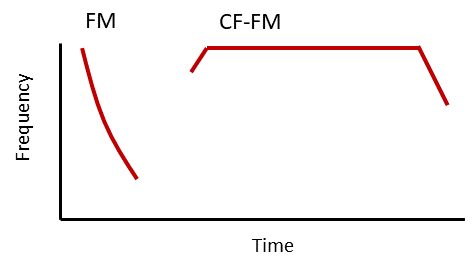
\includegraphics[width=6.61in]{fmcffm-schematic} \caption{\label{fig:cffmschem}Schematic spectrogram showing the call structure of the two broad types of echolocators. Left: A short duration frequency-modulated (FM) call emitted by a low duty-cycle bat. Right: A long duration call with a constant frequency (CF) regions, sandwiched by upward and downward FM regions. The calls are called CF-FM calls.}\label{fig:cffmschem}
\end{figure}

As hinted above echolocation is far from a stereotypical behaviour, with bats showing great flexibility in almost all aspects of their calling behaviour. Take the case of a bat initially searching for prey, locating an insect, capturing it and then resuming flight. As it searches for prey initially, a bat will typically emit high source level, narrow bandwidth, long calls (a few ms) with long inter-pulse intervals (\textasciitilde100-200ms). These call parameters optimise long-range object detection. Upon localising an insect and flying closer, it continues to reduce its call duration and inter-pulse interval, till just before the insect capture the emitted calls are fainter , high bandwidth, shorter (\textasciitilde1ms) and emitted at extremely short inter-pulse-intervals (\textasciitilde5ms). The call parameters in the pre-capture phase are optimised to localise a moving target at close range. The reduced call levels and durations to ensure echoes from background objects do not mask the insect echoes \citep{Fenton2014}. As we will see later, the flexibility in bat echolocation is key to how they may manage flying in groups.

\hypertarget{bats-as-receivers}{%
\subsection{Bats as receivers}\label{bats-as-receivers}}

While sharing many common features with other mammales, echolocating bats show a series of specific adaptations to their aurally dominated lifestyle. Bat hearing thresholds match those of comparable mammals (and humans) at around 20\(\mu\)Pa sound pressure level (SPL) \citep{wahlberg2014sound}. The diverse pinna shapes across bat species contributes to hearing directionality \citep{obrist1993a}, which allows accurate localisation of returning echoes with high angular resolution \citep{Moss1995}. Like humans, and other mammals , bats too undergo forward, backward and simultaneous masking \citep{m1989a, siewert2004a, suemer2009a}. Forward masking is when a `louder' sound (the masker) arrives before the echo and affects detection. Backward masking is when the masker arrives \emph{after} the echo and affects masking. Simultaneous masking is when the masker overlaps the echo, and prevents detection. The combination of forward, backward an simultaneous masking means echo detection is affected even when a masking call arrives a few milliseconds before or after the echo too. To combat masking, bats also show another common auditory phenomenon seen in vertebrates - spatial unmasking \citep{suemer2009a, geberl2019spatial}. Spatial unmasking is the improvement in echo detection with increasing angular separation between masker and echo (despite temporal overlap). For instance \citet{suemer2009a} showed a drop of \textasciitilde26 dB (around 20 fold drop) in required echo level, with a separation of merely 23\(^{\circ}\).

\hypertarget{emitter-receiver-characteristics}{%
\subsection{Emitter-receiver characteristics}\label{emitter-receiver-characteristics}}

The combination of call emission and echo reception properties results in the effective `sensory volume' \citep{nelson2006a} of a bat. Call intensity is highest in front of the bat, and drops with increasing angles to the side. Hearing directionality broadly follows the same pattern. The combined forward bias of both emission and reception systems means that the strongest echoes will arrive in the front, and their detection will also be emphasised too. The forward bias can also be thought of as a `de-cluttering' mechanism, which filters out irrelevant echoes coming from non-target objects \citep{simmons2012biosonar}.

Bats use their combined emission-reception properties to effectively deal with sensory challenge of flying alone too. Clutter is the term used to describe echoes from background objects that hinder target echo detection. Even when echolocating alone, intense echoes from clutter objects can mask the detection of fainter echoes. For instance, a bat attempting to capture an insect in front of a bush will face the problem of having to detect a faint insect echo that is temporally next to a series of loud echoes from the bush. Bats synergestically combine the properties of their emission-reception characteristics along with flight behaviours to optimise object detection \citep{yovel2010optimal, taub2020segregating} under challenging conditions. For instance, bats that needed to land on a target placed in front of a bigger wall approached the target from an angle \citep{taub2020segregating}. This situation closely mimicked the problem of detecting an insect echo in the face of masking clutter echoes. The angled target approach resulted in most of the call's beam being focussed on the target, with a stronger echo from the object and a weaker clutter echo.

\hypertarget{active-sensing-in-noise-and-groups}{%
\section{Active sensing in noise and groups}\label{active-sensing-in-noise-and-groups}}

The robustness of echolocation to noise was an early point of investigation. \citet{griffinresistance} in their paper titled `The resistance of bats to jamming' attempted to overwhelm \emph{Plecotus townsendii} echolocation with an array of 52 speakers playing noise into the flightroom. \citet{griffinresistance} placed thin metal wires into the flightroom and found that the bats were able to succesfully detect and avoid colliding with these wires. Inspired by approaches to RADAR research, \citet{griffinresistance} estimated the signal-to-noise ratio (SNR) a bat might experience, and actually found \emph{negative} SNRs (positive and high values of SNR promise reliable results). Noise playbacks are now an established paradigm in the field \citep{roverud1985discrimination, m1989a, jones1994individual, tressler2009context, hage2013ambient, hage2014ambient, luo2015linking}. One general critcism of noise-based experiments is that the bat auditory system is \emph{not} an electronic sensor where only energy content in a frequency band determines detection. The bat auditory system is capable of discerning the obvious time-frequency structure of an echo from the randomness of ambient noise, and may even be using an efference copy of the emitted call itself as reference \citep{simmons2012biosonar}. Bats' `resistance to jamming' however also remains strong even when conspecific calls are played back from all across a flightroom \citep{amichai2015a}.

What are the bats doing to improve their echo detection? Flightroom and laboratory experiments with playbacks and conspecifics reveal a wide variety of sometimes contradictory echolocation responses across species. Common responses include calling louder and increasing call durations \citep{tressler2009a, m1989a, amichai2015a, luo2015linking}, reducing call rate \citep{adams2017a} or altering bandwidth \citep{hase2016a, hase2018a, hage2013ambient}. Bats have been well studied in their role as `emitters' trying to make the best of a jamming situation. While explanations have been put forward to piece together each species' specific response, a conceptual framework to put together the experience of bats as `listeners' undergoing jamming remains missing.

Flightroom experiments can only simulate the jamming severity of group echolocation to an extent, and are no substitute for studying aggregations in the wild. It is difficult to create a uniformly intense sound field in a room, as already observed by \citet{griffinresistance}. There will always be local pockets of higher and lower sound levels, that an individual bat can make use of. Placing multiple bats in a flightroom is of course the next closest thing to observing groups in the wild. Using live animals then presents the problem of motivating multiple animals to fly simultaneously- which happens less often as one would wish. Along with the lack of animals' motivation, experimenter's have avoided studying large groups (\textgreater5 bats) due to the technical challenge of analysing overlapping calls. Most studies in the lab and field have been with very small group sizes (2-5 bats) \citep{jones1994individual, fawcett2015clutter, fawcett2015echolocation, goetze2016a, adams2017a, hase2018a}. At such small group sizes, it is questionable whether bats experience jamming at all. Are the reported echolocation behaviours responses to jamming, or responses to another moving object in the room \citep[@][]{fawcett2015clutter, fawcett2015echolocation}?. Field observations of larger groups in natural settings have failed to simultaneously capture flight and echolocation behaviour simultaneously \citep{gillam2010a, theriault2010a, cvikel2015a, lin2016a}. There is still much scope for studies accessing the collective behaviour and group echolocation of large bat groups in the wild. While visually driven collective motion has been investigated in great depth in large groups of fish and birds, the study of active sensing bat groups lags far behind.

\hypertarget{technology-in-the-study-of-echolocation}{%
\section{Technology in the study of echolocation}\label{technology-in-the-study-of-echolocation}}

The very discovery of echolocation could only happen because a curious biologist (Donald Griffin) joined a physicist (G.W. Pierce) who had developed an ultrasound detector, and pointed it at the inaudible vocalisations of bats \citep{griffin1958a}. Without stressing too much on the disciplinary labels of the researchers themselves, the moral of the story is that studying echolocation has always meant closely working with technology and forging inter-disciplinary collaborations. Thankfully technology has moved leaps and bounds since the days of Griffin in the 1950's. Reading an account of Griffin's field work \citep{griffin1958a} makes one grateful for the multi-functionality of laptops and smartphones. Griffin had to carry oscilloscope, diesel generator, cameras, film rolls, analog tapes and flash lamps to record a few minutes of data in the field. In contrast I've had to carry laptop, digital soundcards and thermal cameras for fieldwork, all of which weigh far less and with the great advantage of being able to record much much more data.

Some of the challenges still remain the same from Griffin's time onward. Acoustic tracking of bat calls was first achieved by \citet{aubauer1994dreidimensionale}, who used a 4-microphone array. Microphones were placed on a frame, and the time-delays of call arrival between channels were used to triangulate the bat's call position. Since Aubauer's time, multi-microphone arrays have been used to track bats in the lab and field \citep{KOBLITZJENSBARBA, MOSSGHOSE, holderied, SIMMONS, goerlitzpapers}. Acoustic tracking relies on a knowledge of microphone positions, which is achieved by fixing mic positions on frames. The very array-frames that provide stable positions to the microphones are cumbersome especially in the context of fieldwork. Large multi-mic frames need to be carried, assembled, and aligned each time before recordings begin. Animals may inspect these conspicuous objects, instead of showing their regular echolocation behaviour. There is a strong need for flexibility and to do away with microphone array frames based on simple rectilinear geometries.

The positional accuracy of acoustic tracking is dependent on multiple factors such as array geometry, source sound structure and source position. Mathematical derivations of accuracy are intensive and specific to a fixed geometry, as are manual calibration experiments. Estimating tracking accuracy with simulated audio, provides a reliable and fast compromise. Characterising tracking accuracy is important in the planning phase of an experiment, or post-data collection. However, to my knowledge, there are no publicly available tools that allow a user to generate multi-channel data of simulated arrays and sounds.

Aside from the `hardware' issues of placing and planning microphone arrays, certain issues have also remain in the analysis of echolocation data. Many studies still use manual mesurements. Manual measurements are intuitive and yet susceptible to bias. For instance, using spectrograms to measure acoustic parameters can lead to experimenter bias and non-reproducible results \citep{brummspecmanual}. A majority of studies use automated methods to quantify call parameters in the form of inhouse-scripts, whose implementation is only briefly described in the paper. Descriptions are subject to interpretation and description-derived implementations lead to different results \citep{bakervincent2019, mcfee2018open}. There is a strong need for a culture of openly shared, documented scripts and packages in echolocation.

\hypertarget{thesis-outline}{%
\section{Thesis outline}\label{thesis-outline}}

In this thesis I will investigate the sensory challenge faced by active sensing animals in groups using a combination of experimental and theoretical methods. Through modelling I will reveal and quantify the sensory challenge low duty-cycle FM bats face in groups of various sizes. I will then present the results of an field study detailing the echolocation strategies of high duty-cycle, CF-FM bats in the presence of conspecifics. Continuing my focus on field studies, I then report a novel experimental dataset and workflow to study large groups of echolocating bats in the wild. I will end with a series of methodologically driven reports that significantly reduce the effort needed to perform acoustic tracking at scale, help users characterise their microphone arrays and ease the computational reproduciblity of echolocation call analysis.

Echolocation is expected to become increasingly infeasible with growing group sizes due to masking. In response to masking in the form of artificial playbacks and conspecific calls, bats show a variety of changes to their echolocation behaviour. While many experimental studies have reported the changes bats show as `emitters' of sound, very little focus had been given to date on bats as `receivers'. Computational work modelling group echolocation has been restricted to models that are qualitatively based on echolocation, with minimal biological details. In chapter \ref{cpnchapter} I present an experimentally parameterised computational model that estimates the sensory inputs a bat may receive as it echolocates in a group. By quantifying echo detection from small to large groups. I find that even in group sizes of 200 bats, individuals may still be detecting one neighbour every few calls. When alone, a bat detects echoes reflecting off all objects in its surroundings. In contrast to echolocating when alone, bats in groups thus face a much lower `update rate' in groups. Despite this lowered sensory update rate, I argue that the detection of occasional echoes may provide the sensory basis for the impressive feats of collective behaviour bats show in roosting sites, mating swarms and emergences.

Chapter \ref{hbcchapter} takes us into our first experimental study looking at echolocation in groups of high-duty cycle CF-FM bats. Given their longer calls and higher frequency of call emission, the problem of call-echo overlap in CF-FM bat groups is expected to occur already at small group sizes. The issue of call overlaps is also reflected in the audio recordings, which are technically challenging to analyse. Moreover, the study of CF-FM bats in groups has been limited to pairs of bats in flightrooms, with missing field observations of their group echolocation. I fill the gaps in the field by studying the echolocation of \emph{Rhinolophus mehelyi} and \emph{R. euryale} in a natural cave setting. Having developed methods to systematically analyse CF-FM calls (see Chapter (@itsfmchapter)), and approaches to analyse audio with overlapping calls, I quantify the group echolocation of CF-FM bats for the first time in group sizes of upto 4 bats. CF-FM bats do not seem to show major alterations in their call parameters when they fly alone or together in cave settings. Our results highlight the robustness of echolocation as a sensory modality. Bats integrate echo information across multiple calls along with using their spatial memory. When flying in familiar natural settings bats may thus tolerate occasional drops in echo detection, and thus not show major changes in echolocation. Here I add a subtle detail that runs counter to the dominant narrative of echolocating showing dramatic changes in response to jamming.

Emphasising the importance of field studies of active sensing, Chapter \ref{ushichkachapter} describes the methodology, motivation and investigative potential of a novel multi-channel, multi-sensor dataset. The \emph{Ushichka} dataset as I call it, is a series of multi-night recordings of resident FM bats echolocating in a cave chamber next to the sole exit point of the Orlova Chuka cave system. Bats form aggregations in this chamber in groups of 1-\textasciitilde30, and their flight and echolocation behaviour was recorded at high temporal and spatial resolution. Synchronised microphone and camera array recordings allow reconstruction of flight paths and call behaviour. A LiDAR scan of the cave chamber provides the physical context of the exhibited behaviours. Unlike previous studies that have studied groups of bats in the field using either acoustic or 3D video tracking, \emph{Ushichka} is one of its kind in capturing group echolocation with multiple sensors. \emph{Ushichka} opens doors to reconstructing the dynamic sensory inputs of each bat as it flies in the chamber. \emph{Ushichka} adds a unique multi-sensor perspective to collective behaviour in active sensing animals, by providing not only the kinematics, but also insight into the sensory bases of collective movement in bats.

Chapter \ref{sfscotdoa} describes a methodology to automatically infer microphone positions in an acoustic array. While rewarding in terms of the data it generates, the process of setting up a microphone array can be strenuous especially when it comes to taking positional measurements. The use of TotalStation surveying systems that provide direct XYZ measurements are not common in the field (they are themselves another piece of bulky equipment). In contrast to acoustic arrays, camera arrays are much easier to setup and calibrate. Field-friendly protocols like \citet{Theriault2014} mean the field biologist may freely place the cameras, record animal activity and then perform calibrations by moving a common object in front of the cameras. Trying to move away from arrays on frames, I found the work of \citet{zhayida2016automatic} with their `Structure-From-Sound' method. \citet{zhayida2016automatic} were able to automatically infer microphone positions using only the common sounds recorded across channels as input. I was able to initiate a collaboration with Prof.~Åström (Uni. Lund) and convey my enthusiasm for their method when applied to our arrays in the field. This chapter with Prof.~Åström and colleagues shows the viability of automatic microphone position estimation in field conditions, using recordings I made in the Orlova Chuka cave (during \emph{Ushichka} fieldwork described in Chapter \ref{ushichkachapter}). This chapter is but a beginning to the development of field-friendly workflows in acoustic tracking. The `Structure-From-Sound' method used in this chapter and \citet{zhayida2016automatic} promise to significantly reduce the barrier to multi-microphone acoustic tracking for bioacousticians. For one it completely eliminates the need to place microphones in specific geometries on conspicuous bulky frames and secondly, there will be no more need to perform tedious measurements before or after recordings. Being able to handle a larger number of microphones, the bioacoustician will be free to generate even higher resolution measurements of animal sounds.

In Chapter \ref{tacostchapter} I present the \texttt{tacost} software package to aid the design and analysis of acoustic tracking systems. The accuracy of acoustic tracking is affected by multiple parameters, eg. the array geometry, source sound position and signal-to-noise ratios. Experimental calibration of tracking system accuracy is time and labour intensive, while mathematical analysis of accuracy are restricted to specific array geometries. Simulated audio data presents a quick and simple method to estimating the performance of acoustic tracking systems either before or after experiments. \texttt{tacost} generates multi-channel audio data according to user-specified array-related parameters. \texttt{tacost} can be used to plan array geometry to optimise tracking accuracy before experiments, or post-hoc to estimate the accuracy of the tracking system used. I detail the use of \texttt{tacost} to estimate patterns in tracking accuracy with two types of experimentally used array systems, the planar `tristar' array, and an array configuration used in Chapter \ref{ushichkachapter} \& \ref{sfscotdoa} with freely-placed microphones spread around a volume. While \texttt{tacost} does not itself perform any acoustic tracking, it serves as a useful tool to estimate baseline performance. The package is written in the non-proprietary Python language, and released with an open-source license. To ease its use, the package also has detailed online and offline documentation.

In Chapter \ref{itsfmchapter}, I present the \texttt{itsfm} software package originally written to perform systematic and reproducible analysis of CF-FM echolocation calls detailed in Chapter \ref{hbcchapter}. CF-FM calls appear like staple-pins when viewed on a spectrogram. The `rising' and `declining' portions form the frequency-modulated (FM) parts, while the flat portion, forms the constant-frequency (CF) portion (Figure \ref{fig:cffmschem}). The two call portions serve different sensory functions, and can be altered independently. To date, studies have adopted a variety of automated and manual methods to segment and then quantify the alterations in the CF and FM call portions. Manual methods of call segmentation are not reproducible and suscept to experimenter bias, while the automated software based methods remain custom scripts with sparse descriptions. Publicly available implementations are important for the scrutiny and comparison of published methods. Purely description based implementations can show important differences from original implementations. Additionally, none of the software based methods include assessments of segmentation accuracy. \texttt{itsfm} implements a commonly described method (that I call the \emph{peak-percentage} method) to segment CF-FM calls, and introduces a new and more reliable method (the \emph{pwvd} method) to segment CF-FM calls. I also create a synthetic dataset of CF-FM calls, and compare the performance of the \emph{peak-percentage} and \emph{pwvd} algorithms in their segmentation accuracy. Results show that the \emph{pwvd} method is overall superior to the \emph{peak-percentage} method, and is thus the recommended algorithm to use for segmenting CF-FM calls. The \emph{pwvd} method, unlike the \emph{peak-percentage} method, is also potentially applicable to vocalisations of any kind as it does not rely on a specific spectro-temporal shape assumption. The \texttt{itsfm} package is written in the non-proprietary Python language, and released with an open-source license. To ease its use and encourage the further development of the package, detailed online and offline documentation has been made available.

\hypertarget{cpnchapter}{%
\chapter{Modeling active sensing in groups of bats reveals echo detection even in large groups}\label{cpnchapter}}

\chaptermark{Modelling the cocktail-party nightmare}

This chapter was published as a peer-reviewed paper in the Proceedings of the National Academy of Sciences of the United States of America:

\emph{Beleyur, T., \& Goerlitz, H. R. (2019). Modeling active sensing reveals echo detection even in large groups of bats. Proceedings of the National Academy of Sciences, 116(52), 26662-26668.}

\newpage

\hypertarget{cpn_abstract}{%
\section*{Abstract}\label{cpn_abstract}}
\addcontentsline{toc}{section}{Abstract}

Active sensing animals perceive their surroundings by emitting probes of energy and analyzing how the environment modulates these probes. However, the probes of conspecifics can jam active sensing, which should cause problems for groups of active sensing animals. This problem was termed the cocktail party nightmare for echolocating bats: as bats listen for the faint returning echoes of their loud calls, these echoes will be masked by the loud calls of other close-by bats. Despite this problem, many bats echolocate in groups and roost socially. Here, we present a biologically parametrized framework to quantify echo detection in groups. Incorporating properties of echolocation, psychoacoustics, acoustics, and group flight, we quantify how well bats flying in groups can detect each other despite jamming. A focal bat in the center of a group can detect neighbors in group sizes of up to 100 bats. With increasing group size, fewer and only the closest and frontal neighbors are detected. Neighbor detection is improved by longer call intervals, shorter call durations, denser groups, and more variable flight and sonar beam directions. Our results provide a quantification of the sensory input of echolocating bats in collective group flight, such as mating swarms or emergences. Our results further generate predictions on the sensory strategies bats may use to reduce jamming in the cocktail party nightmare. Lastly, we suggest that the spatially limited sensory field of echolocators leads to limited interactions within a group, so that collective behavior is achieved by following only nearest neighbors.

\newpage

\hypertarget{introduction}{%
\section{Introduction}\label{introduction}}

Active sensing animals use self-generated energy to sense their surroundings by analyzing how objects around them change the emitted energy \citep{nelson2006a}. Bats emit loud ultrasonic calls and detect objects around them by listening to the echoes \citep{fenton2013a, griffin1958a}reflected off these objects. Active sensing is an effective sensory modality when the animal is solitary. However, when multiple active sensing animals emit pulses of energy in close proximity, they may ``jam'' each other and mutually interfere with their ability to detect objects in their environment \citep[\citet{matsubara1978a}]{nelson2006a}. If groups of echolocating bats mutually jam or mask each other, they would not be able to detect each other. Due to the intense jamming, individuals would have a progressively difficult time detecting the echoes reflecting off their neighbors, and thus not detect their neighbors at all. Without detecting each other, groups of individuals cannot show collision-free flight. However, many bat species are very gregarious, and fly and echolocate together in groups of tens to millions of bats. Bat groups also show coordinated behaviors in cave flights, evening emergences, and mating swarms \citep[\citet{kunz1982a}]{ortega2016a}. How is their ability to detect each other impaired by increasing group size? How many of its neighbors does a bat actually detect in the presence of intense jamming? What strategies may improve echo detection and thus neighbor detection when many active sensing animals are together? We present biologically parametrized simulations to answer how bats manage to echolocate in the face of intense jamming.

In human psychophysics, the sensory challenge of perceiving an auditory cue among other similar sounds has been called the``cocktail party problem''\citep[\citet{bee2008a}]{cherry1953a}. When applied to bat echolocation, the cocktail party problem has been elevated to the``cocktail party nightmare'', given the high repetition rate, similarity, and amplitude of echolocation calls. On top of these factors is the nonlinear increase in the number of masking sounds with increasing group size \citep{ulanovsky2008a}. Empirical studies to date have investigated the cocktail party problem from a sender's perspective \citep[\citet{ulanovsky2008a}, \citet{brumm2005a}]{bee2008a}. Through field observations, playback studies, and on-body tags \citep{amichai2015a, cvikel2015a, gillam2010a, gillam2016a, lin2016a, ulanovsky2004a, habersetzer1981a, jones1993a, jarvis2013a, adams2017a, falk2014a, surlykke1993a}, we now know a range of echolocation strategies that bats show under challenging acoustic conditions. Bats can increase their call intensity, alter their call duration and frequency range, or suppress calling in the presence of conspecifics and noise playbacks \citep[\citet{adams2017a},\citet{tressler2009a},\citet{m1989a}]{amichai2015a}. In contrast to the many reports of bats' responses to noisy conditions, very little work has been done in conceptually understanding how receiver strategies might contribute to dealing with the cocktail party nightmare \citep[\citet{perkins2017a}]{lin2015a}. To our knowledge, biological modeling of the cocktail party nightmare from a receiver's perspective that includes the details of bat echolocation and auditory processing is lacking. We fill this gap in conceptual understanding by presenting a biologically parametrized model based on the known properties of bat audition and the acoustics of a multi bat echolocation scenario. We quantified how well a bat flying with conspecifics can perceive its neighbors in terms of the returning echoes it detects. Through our simulations, we arrive at a sensory estimate of what a bat in the cocktail party nightmare may be detecting, if anything at all.

\hypertarget{materials-and-methods}{%
\section{Materials and methods}\label{materials-and-methods}}

We model the echolocation of frequency-modulating (FM) bats. The calls of FM bats are typically downward frequency-modulated and of short duration (\(\leq\) 5 ms). Each call is followed by a longer silence (80--150 ms) called the interpulse interval \citep{jones1999a}. FM bats thus sense their world ``stroboscopically'' by emitting a call and listening for the echoes returning during the interpulse interval \citep{griffin1941a}. In the absence of any loud conspecific calls, a bat is able to hear all returning echoes and thus to detect all objects around it. However, in the presence of other loud bat calls, some of its own returning echoes may be masked. In that case, the bat will hear a few or none of the returning echoes. This corresponds to the bat detecting a few or none of the surrounding objects. In the cocktail party nightmare the ``objects'' each bat is trying to detect are its neighbors.

Our model of the cocktail party nightmare is designed to describe the auditory scene \citep{ulanovsky2008a} of a bat emerging from a cave in a group as it echolocates on the wing. A focal bat flying in a group of \emph{N} bats may detect up to \emph{N}-1 of its neighbors (excluding itself), which is equivalent to hearing \emph{N-1} returning echoes. The focal bat receives 2 kinds of loud masking sounds that interfere with the detection of its neighbors: 1) the \emph{N-1} loud calls emitted by other bats in the group, and 2) the secondary echoes created by the call of a neighboring bat, reflecting once off another bat, and arriving at the focal bat. Every neighboring bat call generates \emph{N-2} secondary echoes, meaning that the focal bat can receive up to \emph{N-1}x\emph{N-2} secondary echoes (Figure \ref{cpn_fig1}). We implemented a spatially explicit 2-dimensional (2D) simulation of bat echolocation, sound propagation, and sound reception and include mammalian auditory phenomena to quantify how many and which neighbors a bat can detect in the sonar cocktail party nightmare. We then explored how changes in group size and in sender strategies affect neighbor detection in a group.

\begin{figure}[!htbp]
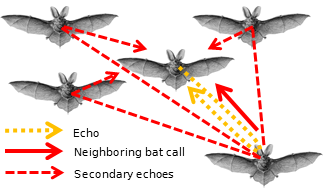
\includegraphics[]{original_papers/CPN_figures/Figure_1/cpn_sounds_schematic_012.png}
\centering
\caption{Schematic of the cocktail party nightmare. Arrows indicate the different types of sounds received by a focal bat: it needs to hear the echoes returning from its own calls (orange) to detect its neighbors, despite the masking by the calls of neighboring bats (solid red) and their secondary echoes (dashed red). Here, only 1 target echo off a single neighbor, only 1 representative neighboring bat call, and its set of secondary echoes are shown. In total, for a group of N bats, the focal bat will receive $N-1$ echoes, $N-1$ neighboring bat calls, and $N-1$x$N-2$ secondary echoes. Bat image courtesy of Wikimedia Commons/Ernst Haeckel.}
\label{cpn_fig1}
\end{figure}

\hypertarget{model-scenarios}{%
\subsection{Model Scenarios}\label{model-scenarios}}

We ran 2 model scenarios to test the effect of 1) increasing group size and of 2) variation in call parameters, group geometry, and acoustic parameters on neighbor detection. In all models, we used the central-most bat in the group as the focal bat.

\begin{itemize}
\tightlist
\item
  Scenario 1: \emph{Effect of group size on neighbor detection:} We simulated groups of 5, 10, 30, 50, 75, 100, and 200 well-aligned bats with identical echolocation and hearing properties flying at a minimum inter-bat distance of 0.5 m (Table \ref{tab:modelscenarios} for full model parameters). The number and location of neighbors detected by the focal bat were recorded in every simulation run.
\item
  Scenario 2: \emph{Effect of call parameters, group geometry, and acoustic parameters on neighbor detection:} Here, we varied other parameters relevant to the cocktail party nightmare (Table \ref{tab:modelscenarios}) while keeping group size constant (\(N_{bats}\)=100, i.e.~the largest group size from Scenario 1 with a biologically relevant neighbor detection rate). We varied call parameters (interpulse interval, call duration, source level), group parameters (heading variation, minimum inter-bat spacing), and acoustic parameters (atmospheric absorption, acoustic shadowing).
\end{itemize}

\begin{table}

\caption{\label{tab:modelscenarios}Model parameters for both model scenarios: Scenario 1 modeled the effect of group size, while other parameters were fixed, resulting in 7 parameter combinations (1 per group size). Scenario 2 modeled the effect of other relevant parameters, while group size was kept constant at 100 bats, resulting in a combined set of 1,200 parameter combinations.}
\centering
\begin{tabular}[t]{>{\centering\arraybackslash}p{4cm}>{\centering\arraybackslash}p{4cm}>{\centering\arraybackslash}p{4cm}}
\toprule
Parameter & Scenario 1: Effect of group size & Scenario 2: Effect of call parameters, group geometry, and acoustics\\
\midrule
Group size & 5, 10, 30, 50, 75, 100, 200 & 100\\
Interpulse interval (ms) & 100 & 25, 50, 100, 200, 300\\
Call duration (ms) & 2.5 & 1, 2.5\\
Source level (dB SPL re 20 $\mu$Pa at 1m) & 100 & 94, 100, 106, 112, 120\\
Minimum interneighbour distance (m) & 0.5 & 0.5, 1.0\\
\addlinespace
Group heading variation ($^{\circ}$) & 10 & 10, 90\\
Atmospheric attenuation (dB/m) & -1 & 0, -1, -2\\
Acoustic shadowing & Yes & No, Yes\\
\bottomrule
\end{tabular}
\end{table}

\hypertarget{model-implementation}{%
\subsection{Model Implementation}\label{model-implementation}}

Each model run simulated 1 interpulse interval of the focal bat, and we calculated the timing and received level of all sounds (target echoes, masking calls, and secondary echoes) that arrived at the focal bat during that interpulse interval. Each model run simulated a series of sounds that arrived during an interpulse interval following the focal bats' call, based on a spatially explicit distribution of a group of bats (SI Appendix, Schematic \ref{cpn_schem_1}). At the beginning of every model run, \emph{N} bats were placed in a 2D space with randomly assigned heading directions (SI Appendix, \ref{cpn_groupgeom} and \ref{cpn_headingvar}). For each neighboring bat, we calculated its angle and distance to the focal bat. The received level was calculated based on a common source level for all bats, spherical and atmospheric spreading over each call's and echo's travel distance, and acoustic shadowing. Acoustic shadowing is the reduction in received level of a sound due to obstructions in its path. A sound in the cocktail party nightmare may pass around obstacles (other bats) as it propagates from source to receiver. The reduction in received level was measured and calculated as a linear function of the number of bats obstructing the path between source and receiver (SI Appendix \ref{cpn_shadowing}). For target and secondary echoes, we also considered monostatic and bistatic target strengths measured in this paper (SI Appendix, \ref{cpn_targetstrength}).

The arrival time of target echoes within the interpulse interval was determined according to the 2-way travel time to the echo-reflecting neighboring bat. The arrival time of masking calls and secondary echoes was assigned randomly with uniform probability across the interpulse interval. The random arrival time assignment of calls and secondary echoes recreates the uncoordinated echolocation of all bats in the group. It is unlikely that multiple bats in large groups can coordinate their calls effectively, and independent calling has been reported even in small groups of 4 bats (\citet{hase2018a}).

All bats in a group were identical in their calling properties, and we treated all sounds as constant tones of equal duration, i.e., we did not explicitly model spectral emission, propagation, and reception properties. The only difference between each of the sounds was their path and source of sound production. The omission of spectral properties is a conservative choice that assumes maximal masking of the primary echoes, thus allowing us to study the role of intensity differences and temporal separation between target echoes and masking sounds.

Once we calculated the timing and received level of all sounds at the focal bat, we accounted for directional hearing sensitivity (SI Appendix, Figure \ref{cpn_figS3}) and spatial unmasking. Spatial unmasking describes the reduction in experienced masking as the arrival angle between masker and target sound increases (\citet{ebata2003a}, \citet{suemer2009a}). We simulated spatial unmasking by the reduction of a masker's effective received level based on its angular separation to an echo. For each echo, the same masker will have a different effective masking level as its relative angle of arrival will be unique for each echo. We thus calculated the effective masking level of each masker for each echo. The effective masking levels of all maskers were then combined to form a time-variant and echo-specific ``masker SPL profile'' (SI Appendix, Figure \ref{cpn_figS5}D). This is essentially the joint sound pressure level (SPL) of all maskers over time. We then expressed this echo-specific masker SPL profile in relation to the echo's SPL, thus obtaining a relative ``echo-to-masker ratio profile'' (SI Appendix,Figure \ref{cpn_figS5}E). This is equivalent to a signal-to-noise ratio profile, where the echo is the signal and the masker profile is the noise.

In addition to angular separation, signal detection is also determined by the temporal separation between signal (echo) and masker (\citet{m1989a};\citet{yost2007a};\citet{siewert2004a}). Masking increases as the masker arrives closer in time to the echo. Masking occurs over longer durations when maskers arrive before the signal (forward masking) than afterward (backward masking). We recreated the asymmetric masking by a ``temporal masking envelope'' temporally centered at the echo (SI Appendix, Figure \ref{cpn_figS1}). The echo was considered heard if the echo-to-masker ratio profile was above the temporal masking envelope. We allowed short drops of the echo-to-masker ratio profile below the temporal masking envelope, for a combined maximum duration of less than 25\% of an echo's duration. Alternatively, we defined an echo to be masked (= not heard), if the echo-to-masker ratio profile was below the temporal masking envelope for more than 25\% of the echo duration. The 25\% threshold was an arbitrarily chosen conservative value to prevent masking by rare and short bursts of high sound pressure level that are unlikely to affect echo detection biologically (SI Appendix, \ref{cpn_detneighbour}).

\hypertarget{model-parametrization}{%
\subsection{Model Parametrization}\label{model-parametrization}}

We implemented a detailed set of echolocation, group and sound properties in our model, including call and hearing directionality, spatial unmasking, temporal masking, group geometry, and details of sound propagation. These properties were parameterized based on published results wherever available. Acoustic shadowing and target strengths (monostatic and bistatic) of bats were specifically measured for this work. All details of the model parameters including our respective measurements and on model implementation are presented in the Supplementary Information.

\hypertarget{results}{%
\section{Results}\label{results}}

\hypertarget{effect-of-group-size-on-neighbor-detection}{%
\subsection{Effect of Group Size on Neighbor Detection}\label{effect-of-group-size-on-neighbor-detection}}

At group sizes of 5 and 10, the focal bat hears the echoes of most or all of its neighbors per call (median: 4 and 8 echoes per call at \emph{N}=5 and 10, respectively; Figure \ref{cpn_fig2}). At progressively larger group sizes, the median number of detected neighbors drops from 4 to 0 at group sizes of 30 to 200. Yet even in a group of 100 bats, while the median number of detected neighbors is zero, the 90th percentile is 1, showing that a neighbor is not detected with each call, but occasionally. Beyond a group of 100 bats, the focal bat typically detects no neighbors at all. The initial rise in detected neighbors in groups of 5 to 30 bats is primarily caused by the increased number of neighbors that could be detected, which is soon counter-acted by the intense masking that rises non linearly with group size.

We next derived the probability of detecting at least 1 neighbor per call, which describes the average rate of neighbor detection (Figure \ref{cpn_fig3}A, blue). At smaller groups of 5 to 30 bats, the focal bat detects at least 1 neighbor per call at above 0.95 probability. At larger group sizes (50 to 100), the probability of detecting at least 1 neighbor drops rapidly to 0.3 per call in a group of 100 bats, and is basically zero for a group of 200 bats (0.004 probability). A bat (with 10 Hz calling rate) flying in a group of 100 bats will thus detect at least 1 neighbor around 3 times per second (\textasciitilde 3 Hz detection rate), while a bat flying in a group of 30 bats will detect at least 1 neighbor almost every time it calls (9.5 Hz detection rate). The probability of detecting multiple bats per call is lower than just detecting at least 1 bat (Figure \ref{cpn_fig3}A). Yet,even in a group of 50 bats, the focal bat has a probability of detecting at least 2 and 4 neighbors per call of about 0.5 and 0.1, respectively.

We next quantified which neighbors the focal bat detects. Detection is generally limited to nearby neighbors (Figure \ref{cpn_fig3}B) and, with increasing group size, to neighbors in front of the focal bat (Figure \ref{cpn_fig3}C). At a group size of 30 bats, the focal bat occasionally detects neighbors that are up to 2 m away in radial distance, which is the furthest neighbor distance. With increasing group sizes, despite the group being more spread out, the focal bat can only detect its nearest neighbors (e.g., neighbors at \textasciitilde0.5 m in a group of 200 bats; Figure \ref{cpn_fig3}B). In the azimuthal plane, at small group sizes, the focal bat initially detects neighbors all around it (95\%-neighbor detection angle range≥237° for up to 50 bats; Figure \ref{cpn_fig3}C). With increasing group size, a frontal bias in neighbor detection appears (95\%-neighbor detection angle range: 191 to 35° for 100 and 200 bats; Figure \ref{cpn_fig3}C).

\begin{figure}[!htbp]
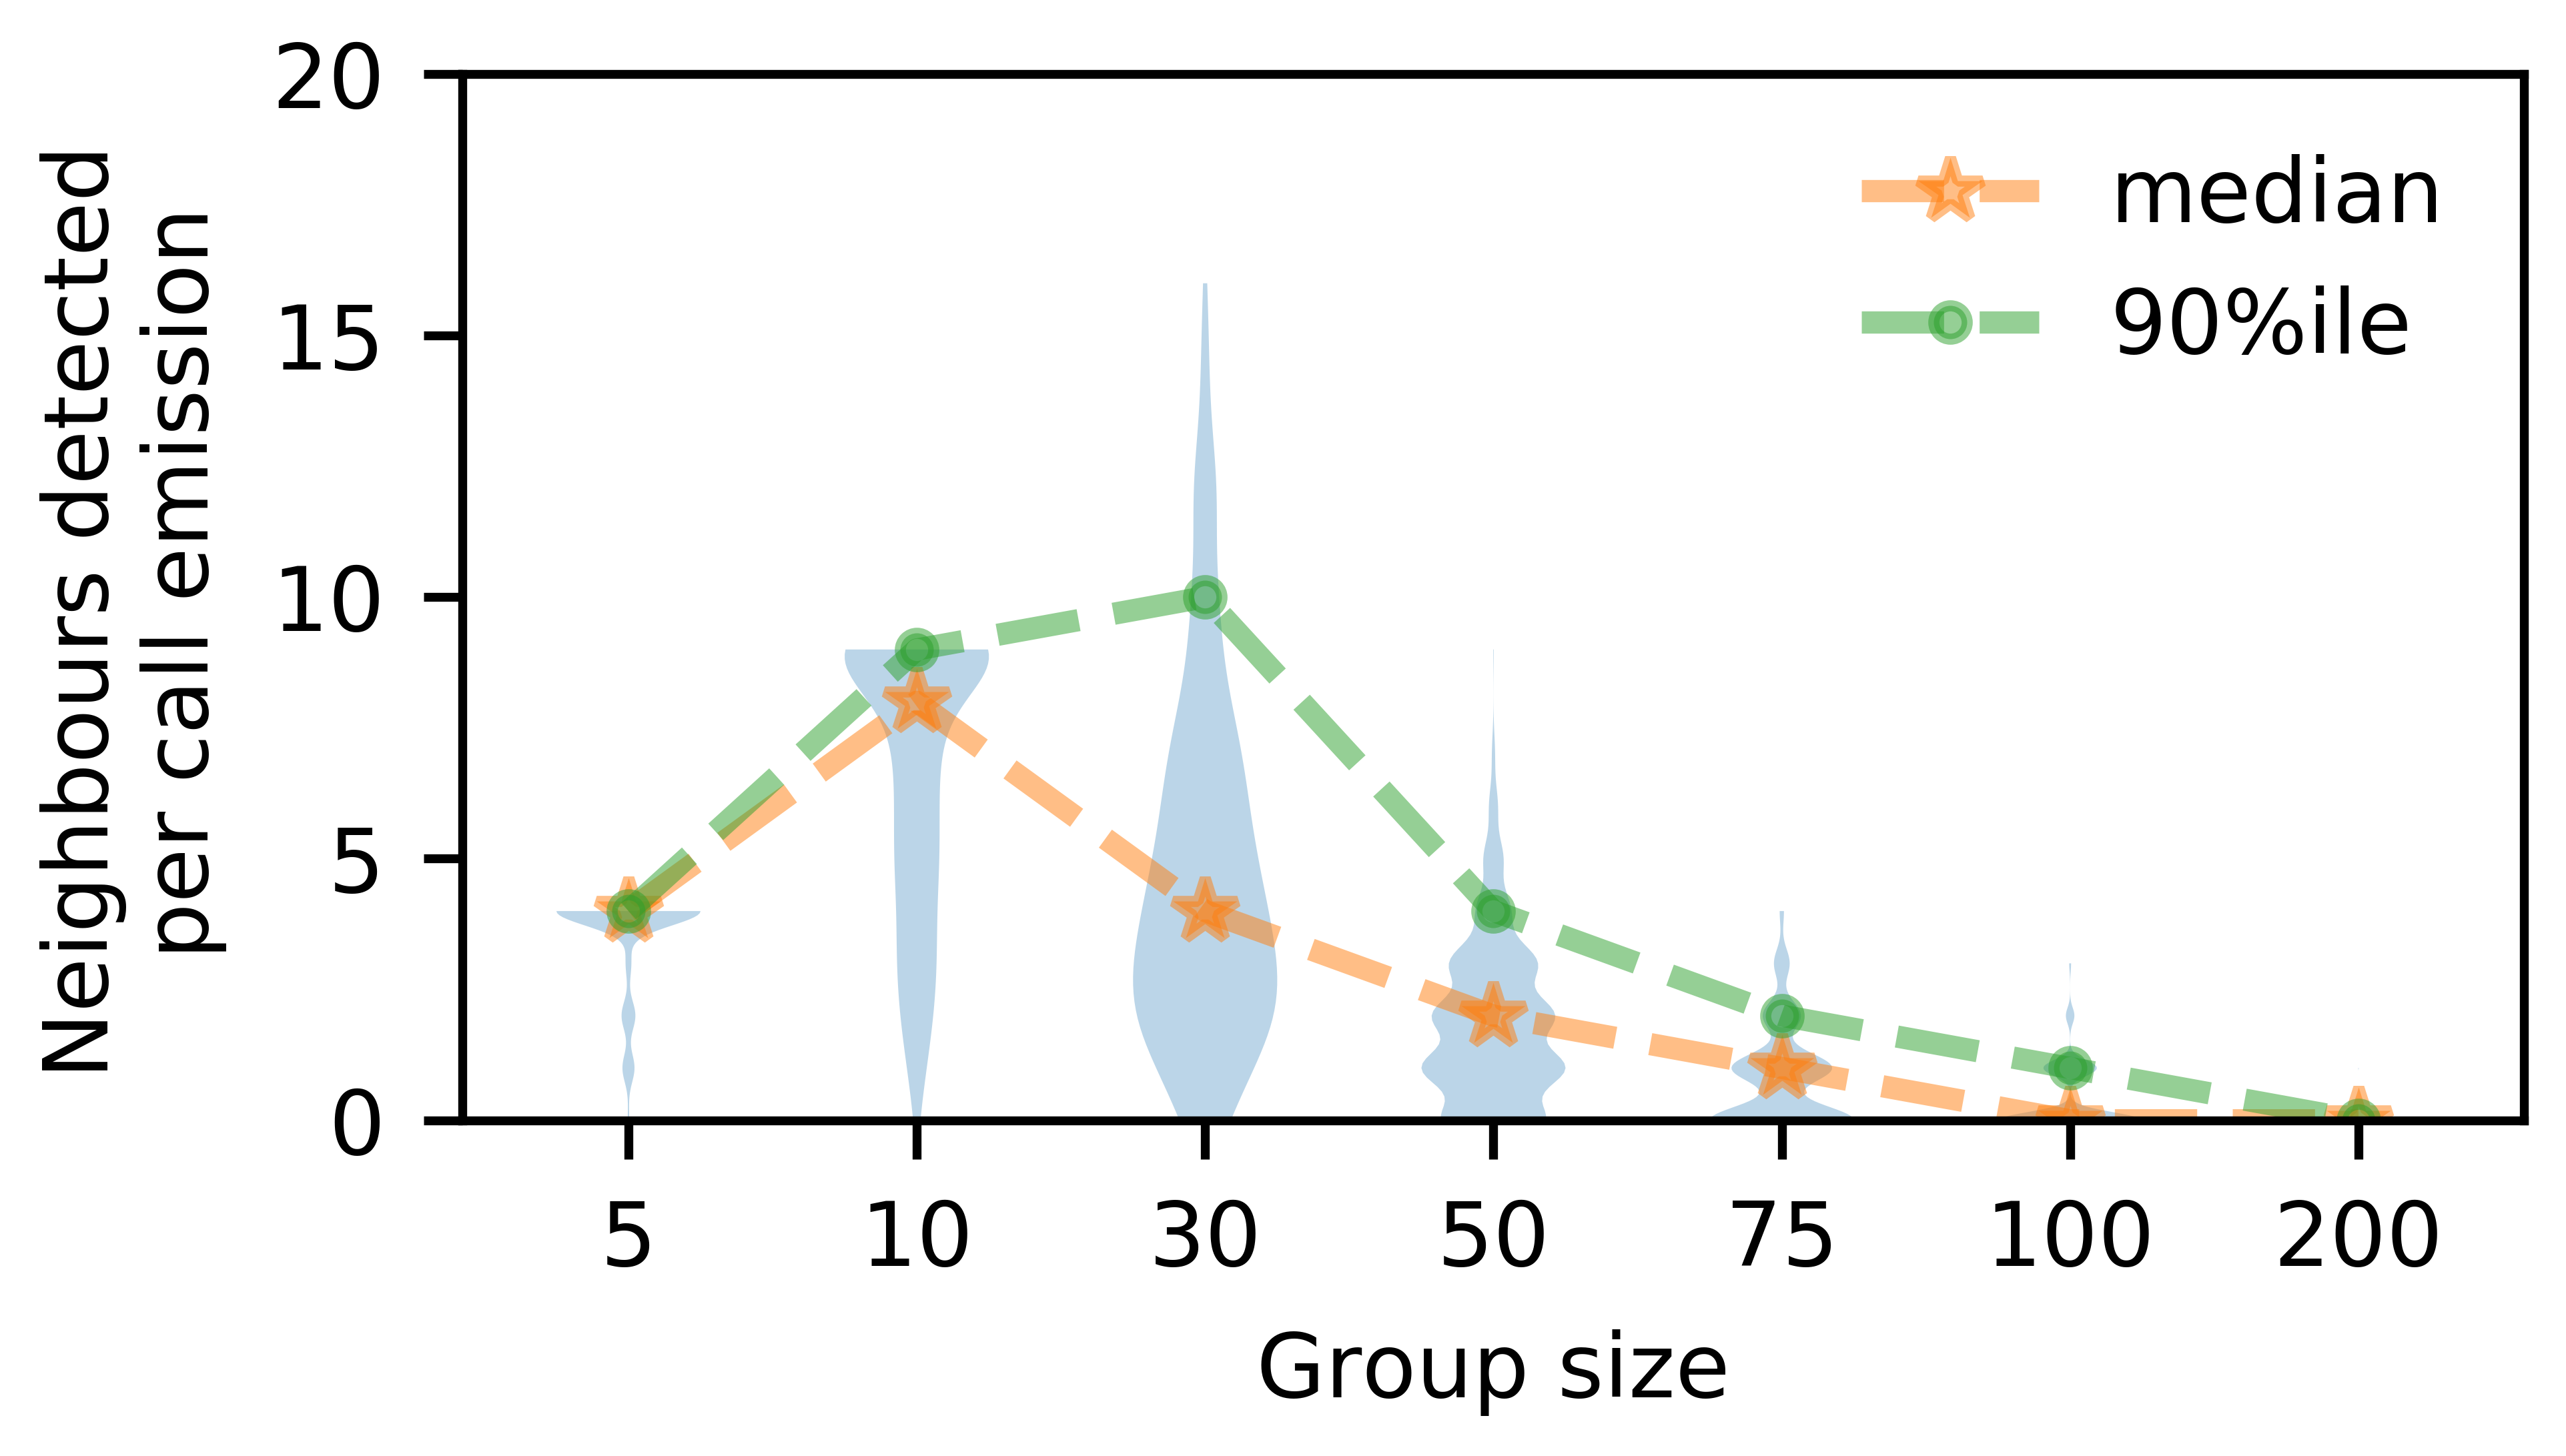
\includegraphics[]{original_papers/CPN_figures/Figure_2/Figure2_groupsize_1200dpi.png}
\centering
\caption{Number of detected neighbors per call by a focal bat in the center of a group. The initial rise in the number of detected neighbors is because there are indeed more neighbors and the degree of masking is low. However, with increasing group size, most of the neighbors cannot be detected anymore, and progressively fewer neighbors are detected per call. Violin plots show the distribution of the number of neighbors detected per call, and their median (stars, orange) and 90th percentile (dots, green).}
\label{cpn_fig2}
\end{figure}

\begin{figure}[!htbp]
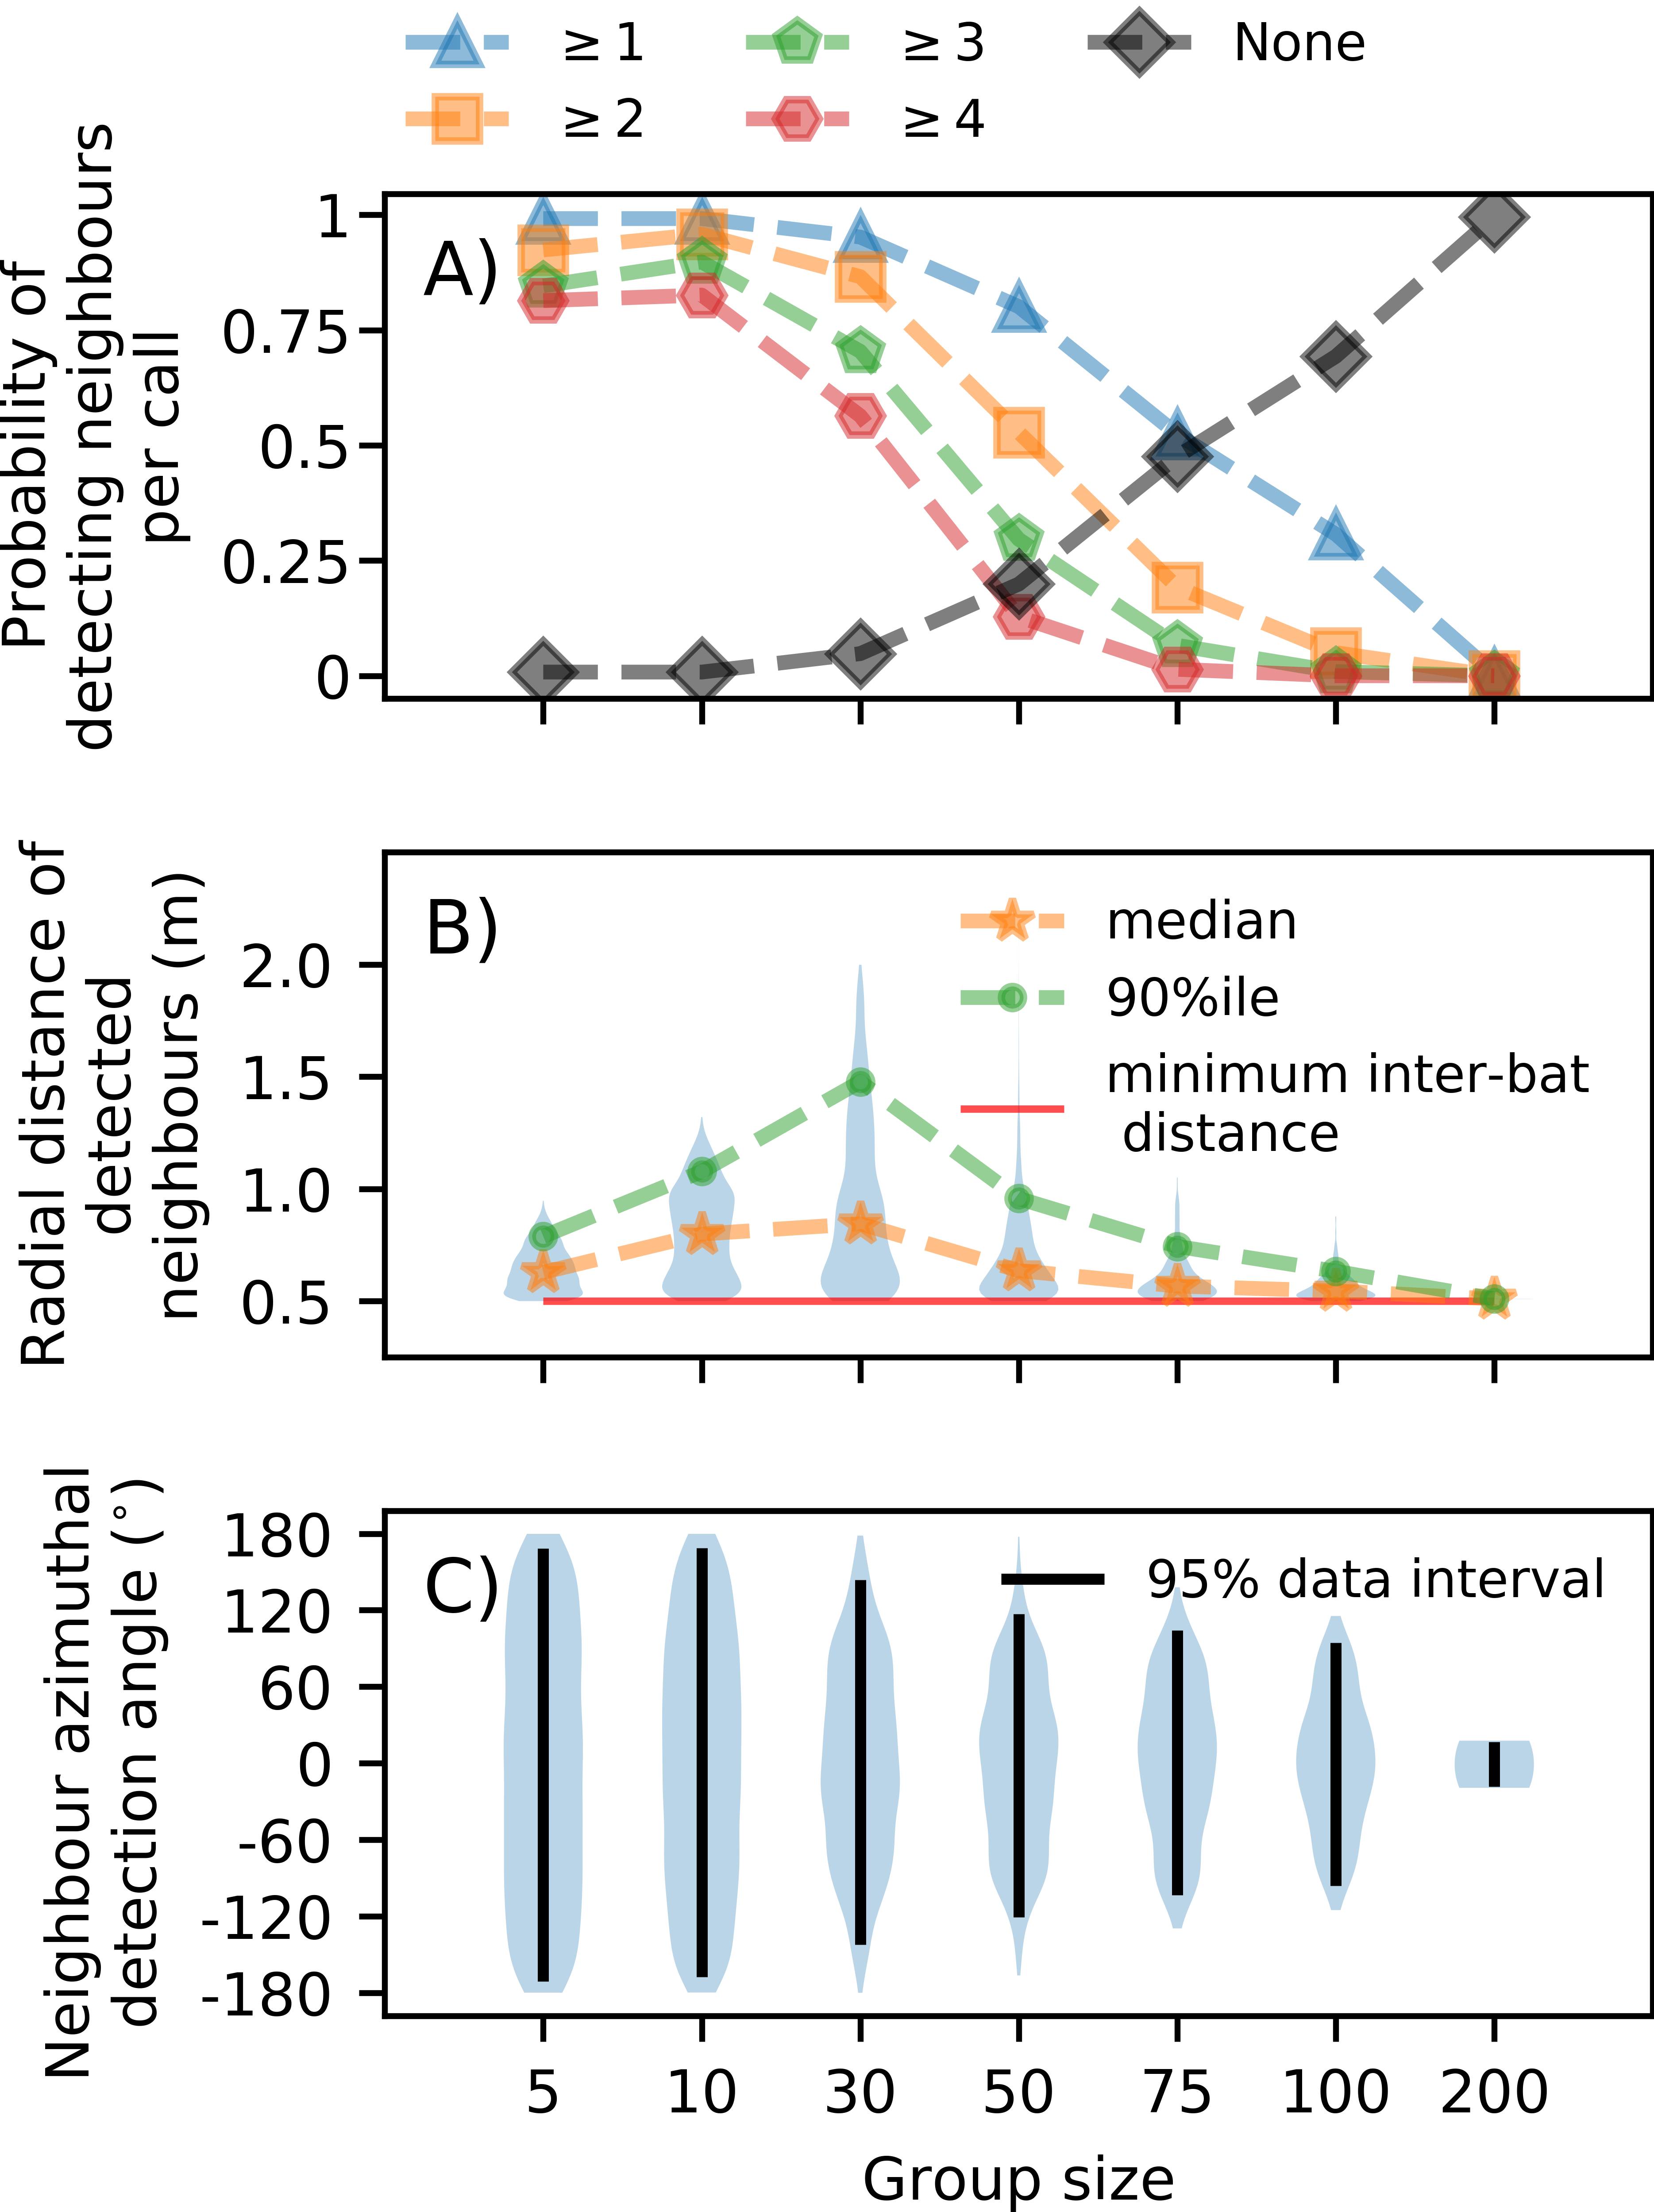
\includegraphics[]{original_papers/CPN_figures/Figure_3/Figure3_1200dpi_tight.png}
\centering
\caption{Characterization of the focal bat’s perception. (A) The probability of detecting $\leq X$ neighbors per call ($X$ = 1,2,3,4, or none). Even in groups of up to 100 bats, the focal bat has a \textasciitilde0.3 probability of detecting at least 1 neighbor
per call. In even larger groups (200 bats), no neighbors are detected anymore. (B) With increasing group size, a focal bat only detects its closest neighbors. Initially, the radial distance of detected neighbors increases because the spatial extent of a group increases with group size (at 5, 10, 30 bats: radius = 0.75, 1.12, 1.97 m), but it then drops down to the nearest neighbors beyond 30 bats. (C) The azimuthal location of detected neighbors, showing an increasing frontal bias with increasing group size. Although neighbors were uniformly distributed in azimuth, the frontal bias of call and hearing directionality means that frontal returning echoes are louder than peripheral ones.} 
\label{cpn_fig3}
\end{figure}

\hypertarget{effect-of-call-parameters-group-geometry-and-acoustic-parameters-on-neighbor-detection}{%
\subsection{Effect of Call Parameters, Group Geometry, and Acoustic Parameters on Neighbor Detection}\label{effect-of-call-parameters-group-geometry-and-acoustic-parameters-on-neighbor-detection}}

We next analyzed how variation in call parameters, group structure, and acoustic parameters affected neighbor detection. We fixed the group size to 100, as at this size, the focal bat could typically detect at most 1 neighbor (90\%ile, Figure \ref{cpn_fig2}) at 0.3 probability (Figure \ref{cpn_fig3}A) per call. We thus reduced the output of each simulation run to a binary neighbor detection score of 1 (detection) or 0 (no detection). We analyzed the effect of each parameter on neighbor detection with a logistic regression, treating all parameters as categorical and using their value in Scenario 1 as reference (parameter range in Table \ref{tab:modelscenarios}).

The call parameters interpulse interval and call duration showed the strongest effect (Figure \ref{cpn_fig4}A,B and SI Appendix, Table \ref{tab:regressionresults}\}). Increasing the interpulse interval from 100 ms to 200 and 300 ms increases neighbor detection probability by about 15 and 75 times, while reducing it to 50ms lowers neighbor detection to 0.05 times that of Scenario 1 (Figure \ref{cpn_fig4}A). Shortening call duration from 2.5 ms to 1 ms led to 35 times higher neighbor detection (Figure \ref{cpn_fig4}B). Call source level had no effect (Figure \ref{cpn_fig4}C).

Group geometry also influenced neighbor detection probability, but less than changing call parameters. Flying at larger interbat distances of 1.0 m leads to 0.31 times lower neighbor detection compared to denser groups with 0.5 m interbat distance (Figure \ref{cpn_fig4}D). Groups where individuals head in a more variable direction have 1.32 times better neighbor detection than groups with a generally common heading (or echolocation beam) direction (Figure \ref{cpn_fig4}E).

Among the physical parameters, acoustic shadowing increased neighbor detection (without acoustic shadowing, neighbor detection is 0.75 times lower than with acoustic shadowing), while atmospheric attenuation had a negligible effect (Figure \ref{cpn_fig4}F and G).

\begin{figure}[!htbp]
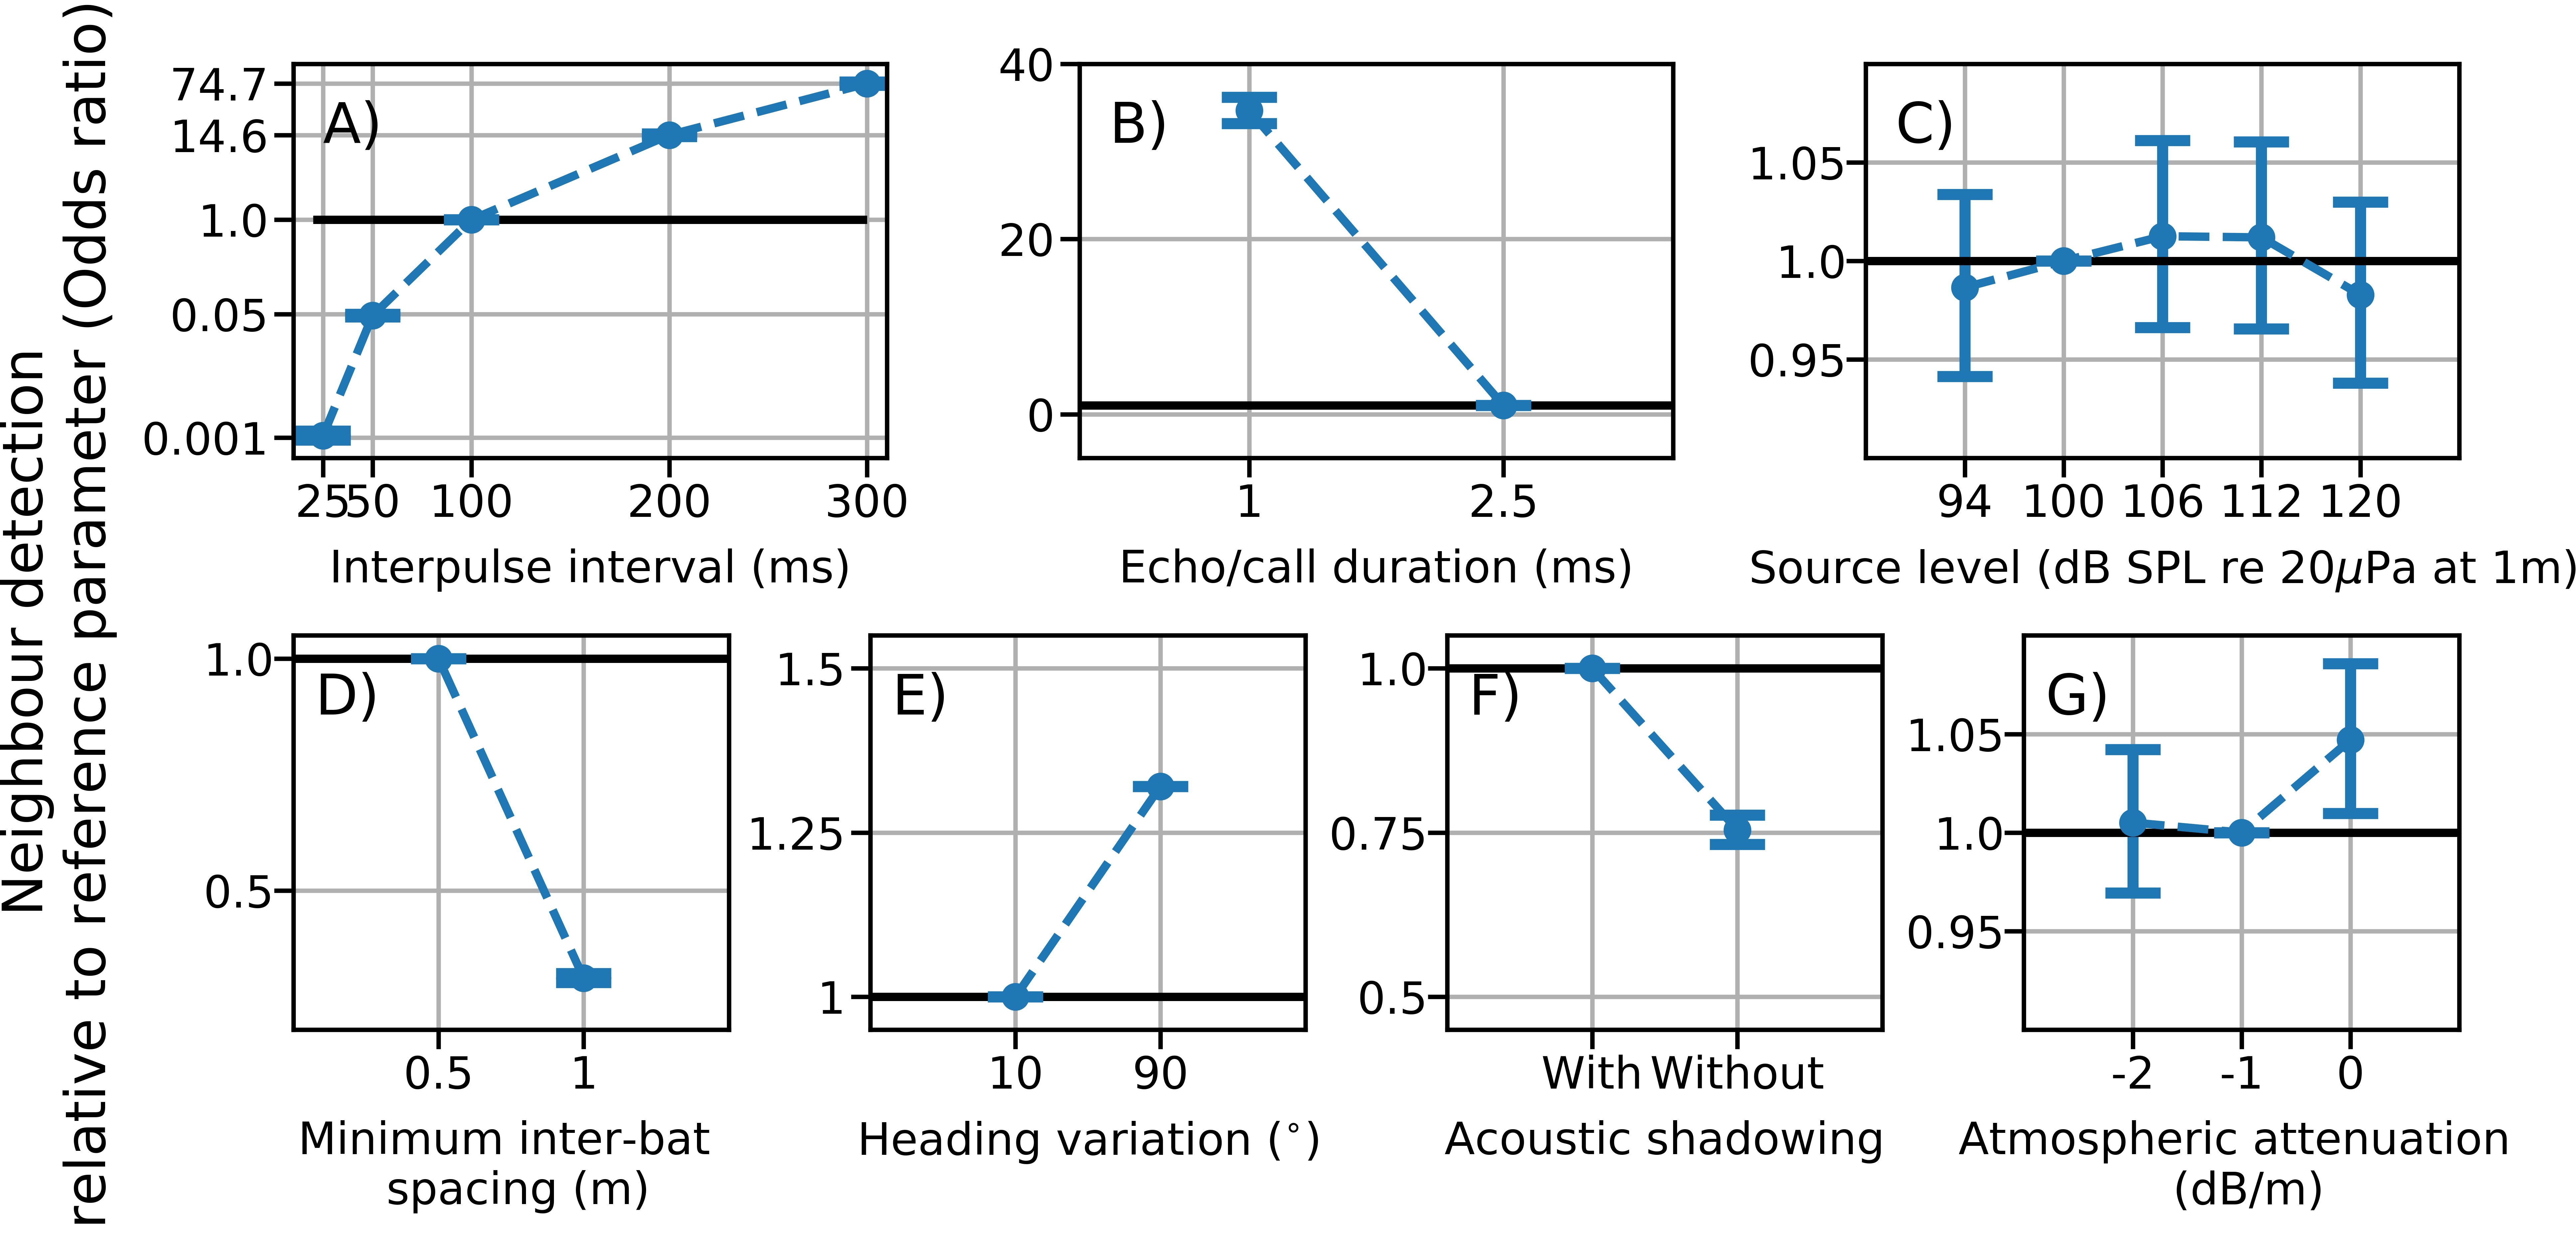
\includegraphics[]{original_papers/CPN_figures/Figure_4/Figure4_oddsratio_comparison.png}
\centering
\caption{Effect of call parameters (A–C), group geometry (D and E), and acoustic parameters (F and G) on neighbor detection. Each plot shows the probability of neighbor detection (model estimate and 95$\%$ confidence interval of odds ratio) when changing model parameters relative to the reference parameter used in the simulations of Scenario 1 (Table \\ref{tab:regressionresults}). Odds ratios above and below 1 indicate a higher and lower neighbor detection probability, respectively, indicated by the horizontal reference line. (A–C) Call parameters: Longer interpulse intervals (A) and shorter call durations (B) increase neighbor detection probability, while call source level (C) has no effect. (D and E) Group geometry: Neighbor detection is better in groups that are tightly packed (D) and with higher heading variation (E). (F and G) Effect of acoustic parameters: Acoustic shadowing by bats in groups improves neighbor detection probability (F), while atmospheric attenuation has a negligible effect (G)} 
\label{cpn_fig4}
\end{figure}

\hypertarget{discussion}{%
\section{Discussion}\label{discussion}}

We present a conceptual framework to quantify what a focal bat experiences in the sonar cocktail party nightmare. We quantified the probability of detecting neighbors across a range of group sizes, which allows calculating the rate at which a focal bat detects its neighbors. When flying alone, a focal bat will detect objects around it at a rate equal to its call rate, while in a group, its object detection rate is reduced due to masking. We show that even in a group of 100 bats, bats still detect at least 1 neighbor per call about 3 times per second (for a 10 Hz call rate), while in smaller group sizes, neighbor detection rate is larger at 5 to 10 Hz. Bat echolocation is generally ``stroboscopic,''meaning that information is received intermittently with time gaps \citep{griffin1958a}. We suggest that bats in smaller group sizes still experience a sufficiently high information update rate for performing collision avoidance and neighbor following. With increasing group size, perception might become ``hyper-stroboscopic'', i.e., so scarce that different sensorimotor heuristics might be required to maintain group coordination.

The low level of masking at smaller group sizes allows the focal bat to detect all its neighbors per call. With increasing group size, however, the focal bat detects maximally 1 neighbor per call in a group of 100 bats. This neighbor detection rate of at least 1 neighbor per call even in large group sizes provides a formal sensory basis for group movement in active sensing animals. While a bat in a large group cannot track the position of all its neighbors, it still can track the movement of a few neighbors, specifically those close to and in front of it. This reduction in rate, range, and direction of detected neighbors has predictive consequences for the kind of collective behavior bat groups may show in nature. Many models of collective movement assume that each individual in a group detects the position and orientation of neighbors in the whole of its sensory volume, and then performs an averaging across all neighbors to decide its next movement \citep{couzin2002a, g2004a, t1995a, reynolds1987a}, leading to the impressive coordinated behaviors of fish schools and insect swarms \citep{sumpter2006a, vicsek2012a}. As the number of neighbors that an individual detects decreases, more ``limited interactions'' begin to dominate, causing anisotropy in the group structure \citep{bode2011a, ballerini2008a}. For bats in the cocktail party nightmare, we predict that large groups may show higher anisotropy than smaller groups due to the limited number of neighbors that they can detect and react to. All things being equal, we predict that in large groups (\textgreater50 bats), the neighbors in the frontal field of a bat will have a disproportionate influence on its movement decisions. Bats in larger groups may thus maintain higher alignment with their frontal neighbors compared to bats in smaller groups.

Our simulations allow for a direct quantitative comparison of the effects of echolocation, group geometry, and acoustic parameters in group echolocation. Among the call parameters tested, reducing call rate (increasing interpulse interval) was most effective in increasing neighbor detection in jamming conditions, matching experimental evidence for reduced calling rate in \emph{Tadarida brasiliensis} \citep{jarvis2013a, adams2017a}. In contrast, other FM bat species increase their call rates in groups and background noise\citep{amichai2015a, lin2016a, cvikel2015b, luo2015a}. Likewise, our result that shorter call duration should improve neighbor detection is opposite to experiments showing that most bat species increased call duration in the presence of maskers \citep{amichai2015a, tressler2009a, m1989a, luo2015a, hase2016a}, except \citep{cvikel2015b}. Lastly, our result of no effect of changing source level on neighbor detection might also seem to differ from experimental data showing that bats in laboratory conditions do increase source level in the presence of maskers \citep{amichai2015a, tressler2009a, luo2015a, hase2016a}. While there might be species-specific variation, we suggest that these differences are mostly due to the experimental situation. Bats in these experiments experienced constant maskers. Calling more often, for longer, and louder thus improved the bats' signal redundancy, echo-to-masker ratio, and overall echo detection. In contrast, our model simulates group flight of many bats with simultaneous and uniform changes in their call parameters. When all bats in a group shorten call duration, this reduces the overall duration of masking sounds, thus improving echo detection. Likewise, when all bats in a group increase their call amplitudes to optimize their own echo-to-masker ratios, all bats will eventually call at their maximum, with no overall effect on neighbor detection. Analyzing bat calls in mass emergences is technically challenging and it remains unknown whether \emph{T. brasiliensis} and other gregarious bat species reduce their call rate in the field.

Bat aggregations show a variety of structures across behavioral contexts, from well-aligned almost parallel flight during roost emergences, to more variable and less-aligned flight in mating swarms and when circling in limited cave volumes. We show that this group structure itself affects how well bats can detect each other. Bats detect their neighbors better in less-aligned groups compared to more aligned groups. During aligned emergence flight, the focal bat always receives loud forward-directed masking calls from bats behind it, in addition to the relatively loud side-calls emitted by neighbors to its left and right. In contrast, during less-aligned swarming flight, the relative orientation of the bats is more distributed and changing, with the focal bat experiencing a wider dynamic range of masker levels (i.e., louder and fainter masking calls originating from a wider range of angular directions). This increased dynamic masker range allows for better echo detection, as there will be drops in echo-to-masker ratios due to changing received masker level. This effect is beneficial for enabling swarming flight, as the collision risk in less-aligned flight is likely higher compared to the more aligned emergence flights. Inter-individual distance is another parameter of group structure, and we show that neighbor detection is better in dense groups. This might seem unexpected given that the received SPL of the maskers is higher the closer the bats are to each other. However, received echo levels are also higher when bats are closely spaced. Since echo SPL drops by 12 dB per doubling of distance, but masker call SPL only by 6 dB per doubling of distance, the echo-to-masker ratio is higher at shorter compared to longer inter-bat distances. It would be interesting to examine if perhaps large groups in the field actually fly closer to each other than smaller groups.

While we only modeled neighbor detection for the central-most bat in a group, its position in the group (e.g., central, frontal, or at the back) is likely to also have an effect on the number and received level of maskers, and thus on the number of detected echoes. However, we expect the obtained trends to remain qualitatively the same regardless of focal bat position. Particularly, we predict that masking will increase with group size, and only the exact group size at which a given level of masking (e.g., X\% neighbor detection probability) is obtained will change depending on the focal bat's position in the group.

We furthermore show that it is important to consider bats not only as sources of reflected echoes and masking sounds, but also as obstructions to sound that actually alleviate the cocktail party nightmare. Typically, the detected echoes originate from nearby bats and are not shadowed. In contrast, the masking calls and secondary echoes can arrive from distant neighbors, thus passing by multiple other bats. Shadowing thus consists of the overall reduction in masker levels, which increases echo-to-masker ratios for the comparatively loud echoes returning from nearby neighbors.

Our results show that the cocktail party may not be as much of a ``nightmare'' as previously thought \citep{ulanovsky2008a}. We show that the modeled psychoacoustic, spatial, and acoustic properties act together to alleviate the nightmare into a challenge. When bats are flying in a multi echo environment, our results show that a bat will always hear some echoes after a call emission, and very rarely no echoes at all. This parallels the phenomenon of auditory ``glimpsing'' reported in the human auditory cocktail party where individuals may follow conversations by perceiving parts of detected speech rather than whole sounds \citep{miller1950a}.

\hypertarget{improved-echo-detection-in-real-world-situations}{%
\subsection{Improved Echo Detection in Real-World Situations}\label{improved-echo-detection-in-real-world-situations}}

We present a first approximation to the sonar cocktail party nightmare, including many relevant biological, physical, and auditory mechanisms. Bats are expert echolocators and can detect echoes and fly under challenging conditions \citep{m1989a, surlykke1992a, petrites2009a, bates2008a}. Bats rapidly adjust their call behavior in terms of their call duration, source level, and interpulse intervals \citep{luo2017a, corcoran2017a}, integrate echoic information over multiple call emissions \citep{simmons2012a}, and actively track objects by aiming their calls at them \citep{ghose2006a, ghose2006b}. While we tested a range of differentecholocation call parameters, our model implemented these parameters as fixed values that do not vary over time, thus lacking the dynamic nature of a real bat in the wild.

Furthermore, we did not model the spectral content of echo ormasker sounds, and analyzed echo detection based on a fixedthreshold of echo-to-masker-ratio. In contrast, real echolocation calls possess a time-variant spectral pattern that is species and even individual specific \citep{gillam2010a, yovel-a}, which can reduce echo masking. Masking is strongest when target and masker overlap both intime and in frequency (i.e., fall within the same critical band ofthe auditory system) \citep{ebata2003a, fletcher1940a}. The frequency-modulation of bat calls means that even when maskers and echoes partially overlap in time, they will not necessarily overlap in frequency, thus reducing the likelihood of masking. The individuality of bat calls may help a bat reject the secondary echoes from other bats' calls by forming separate auditory streams \citep{fay2008a} for its own echoes and others' echoes. Given the scarcity of empirical data to parametrize the effect of spectral differences on echo detection in masking conditions, we did not include it in our model, thus simulating a conservative worst case scenario where all sounds lie in the same frequency band. Additionally, attentional processes strongly improve target detection by improving the signal-to-noise ratio in the presence of maskers with similar time-frequency structure \citep{hafter2008a}. Under real-world conditions, it is likely that masking in groups is even less than simulated here.

Due to the scarcity of published data, the inter-individual and interspecific variation in the temporal and spatial masking functions used in our model is unknown. The temporal masking envelope will arguably be similar in many bat species, showing the typical mammalian pattern of worse target detection threshold with shorter temporal separation between target and masker. Spatial unmasking occurs through the nonlinear interaction of pinnae shape, cochlear and higher auditory processing \citep{ebata2003a, culling-a}. As pinna shape and associated acoustic receiver characteristics strongly vary in echolocating bats \citep{obrist1993a}, this will lead to species-specific spatial unmasking and echo detection rates in the sonar cocktail party nightmare.

\hypertarget{conclusion}{%
\section{Conclusion}\label{conclusion}}

We provide a conceptual framework to explain how active sensing animals such as echolocating bats successfully navigate in groups despite mutually jamming each other. The intense jamming in groups might lead to individuals only detecting their nearest frontal neighbors, which might drive limited interactions within a group. We also show that call parameters and group geometry determine the challenge in the sonar cocktail party nightmare. Recent advances in on-body acoustic tags \citep{cvikel2015b, stidsholt2018a}, signal analysis \citep{aodha2018a}, and acoustic tracking \citep{seibert2015a} of echolocating animals in the field might facilitate future experimental validation of our model predictions. As our model formulation is not constrained to echolocation in bats, it can be parametrized to other echolocators such as oilbirds, swiftlets, and odontocetes \citep{brinkl2013a, surlykke2014a} that also echolocate in groups and suffer from cocktail-party--like conditions.

\hypertarget{acknowledgements}{%
\subsection{Acknowledgements}\label{acknowledgements}}

We thank the members of the Acoustic and Functional Ecology Group for insightful comments and support, Claire Guérin for contributing to code development, the Max Planck Institute for Ornithology for excellent research infrastructure, and 2 anonymous reviewers for helpful comments. T.B. was funded by a doctoral fellowship from the German Academic Exchange Service (DAAD) and the International Max Planck Research School for Organismal Biology. H.R.G. was funded by the Emmy Noether program of the German Research Foundation (DFG, GO 2091/2-1, GO 2091/2-2).The simulation runs in this paper were funded by a Google (Research Credits) grant to T.B.

\newpage

\hypertarget{supplementary-information}{%
\section{Supplementary Information}\label{supplementary-information}}

\hypertarget{model-parametrization-1}{%
\subsection{Model parametrization}\label{model-parametrization-1}}

Here, we present the details of how we parametrized our model of the sonar cocktail party nightmare, based on empirical data of behavioral studies in bats and our own measurements.

\hypertarget{temporal-masking-envelope}{%
\subsubsection{\texorpdfstring{Temporal masking envelope \label{cpn_tempmasking}}{Temporal masking envelope }}\label{temporal-masking-envelope}}

We derived the echo-to-masker sound pressure level (SPL) ratios for forward, backward and simultaneous masking from two empirical target-detection studies in echolocating bats (Table \ref{tab:maskingtable}). We only chose studies where the target and masker were co-located along the same direction. Both studies presented the ratio between the echo and masker SPL at target detection for various delays between
echo and masker arrival time. We linearly interpolated (in a piecewise fashion) the echo-to-masker SPL ratios between each of the time delays measured in the studies to obtain the full temporal masking envelope ranging from -0.65 and +24 ms delay of the target echo relative to the masker edge (Figure \ref{cpn_figS1}).

\hypertarget{spatial-unmasking-function}{%
\subsubsection{\texorpdfstring{Spatial unmasking function \label{cpn_spatiunmasking}}{Spatial unmasking function }}\label{spatial-unmasking-function}}

\citet{suemer2009a} performed a backward masking study to address spatial unmasking in the bat \emph{Eptesicus fuscus}. In a two-alternative forced-choice paradigm, they increased the angular separation between a target object and a masker object while also varying the level of the target object's echo (by varying the size of the target object and thus its target strength).

We define the spatial unmasking function as the echo-to-masker SPL ratio at just-noticeable echo detection as a function of angular separation. To obtain the echo-to-masker level ratios, we subtracted the target object's target strengths from the masker object's target strength. We normalized the spatial unmasking function to the co-localised echo-masker case (i.e., when both echo and masker arrive from the same direction). This describes the reduction in echo-to-masker ratio required for echo detection as a function of angular separation between target and masker,compared to the co-localized case. We digitized the data points from Figure \ref{cpn_fig4}B of Sümer et al.~(2009) by hand with WebPlotDigitiser \citep{rohatgi2015a} to obtain the target's target strength as a function of angular separation. Masker target strength was given by \citet{suemer2009a} as -14.5 dB. We then calculated the target-masker SPL ratios and interpolated them with a quadratic polynomial fit (Figure \ref{cpn_figS2}). The interpolated data was then further upsampled to 0.47° intervals. As \citet{suemer2009a} only measured angular separations up to 23°. We conservatively used the echo-masker SPL ratio at 23° also for all larger angular separations.

\hypertarget{call-and-hearing-directionality}{%
\subsubsection{\texorpdfstring{Call and hearing directionality \label{cpn_directionality}}{Call and hearing directionality }}\label{call-and-hearing-directionality}}

Echolocation calls have a directional beam shape, meaning that the emitted SPL
generally decreases with increasing angular distance from the main call direction, which has the highest call SPL (Figure \ref{cpn_figS3}). The highest call SPL is typically towards the front, and reduces towards the back of the bat. Despite this directionality and additional variation with call frequency and behavioral context \citep{jakobsen2010a, l2013a, surlykke2012a, giuggioli2015a} , bats still emit a significant amount of sound pressure into the backward direction. The average call SPL behind a bat is about 14 dB lower than in the forward direction \citep[\citet{stidsholt2018a}]{giuggioli2015a}. Call directionality leads to a drop in the effective number of masking calls from neighbors as only those calls arriving from a limited range of directions will have sufficiently high SPL (Figure \ref{cpn_figS3}). For example, in an emergence situation with approximately parallel flight directions, the focal bat will receive the loudest calls from those bats flying behind it. Similarly, the lowest received call levels in an emergence will be from those bats flying in front of the focal bats.

Like call production, hearing is also directional. The pinna structure of a bat
attenuates or amplifies the same sound depending on its direction of arrival \citep[\citet{f2008a}]{firzlaff2003a}. In \emph{Myotis daubentonii}, hearing directionality between 35-45 kHz leads to an average amplification of frontally arriving sounds by 4 dB in comparison to those arriving from behind. We used data of \citet{giuggioli2015a} to describe the average call and hearing directionality of our modelled bats (Figure \ref{cpn_figS3}).

\hypertarget{atmospheric-attenuation}{%
\subsubsection{\texorpdfstring{Atmospheric attenuation \label{cpn_atmabs}}{Atmospheric attenuation }}\label{atmospheric-attenuation}}

Ultrasound in air is heavily attenuated by atmospheric attenuation, even over short distances of a few meters \citep[\citet{lawrence1982a}]{h2018a}. Atmospheric attenuation will reduce the received SPL of a masker or echo at the focal bat. We chose a range of values for the atmospheric attenuation coefficient \(\alpha\) between 0 to -2 dB/m. These values approximate the atmospheric attenuation experienced by a bat calling at very low (\(\leq\) 20 kHz, \textasciitilde0 dB/m) to high (60 kHz, \textasciitilde-2 dB/m) peak frequencies.

\hypertarget{geometric-attenuation}{%
\subsubsection{\texorpdfstring{Geometric attenuation \label{cpn_geomattn}}{Geometric attenuation }}\label{geometric-attenuation}}

Sound pressure level reduces with increasing distance from the source, called geometric attenuation. For all sounds in our model (target echoes, masking calls and secondary echoes), we implemented spherical geometric spreading, i.e.,uniform spreading of sound in all directions \citep{speaks1996a}.

\hypertarget{group-geometry}{%
\subsubsection{\texorpdfstring{Group geometry \label{cpn_groupgeom}}{Group geometry }}\label{group-geometry}}

A group of bats might organize themselves tightly or well spread in the field. The spacing between bats will decide how loud the returning target echoes, masking calls and secondary echoes are. We simulated a group of bats by placing individual bats on a 2D plane using the Poisson disk algorithm \citep{bridson2007a}. The advantage of using the Poisson disk algorithm is that points are spaced relatively uniformly in space compared to a random placement of points from two independent distributions. The other advantage of the Poisson disk algorithm is that it allows the specification of a minimum distance between two points. For the first simulations varying group size only, we chose 0.5 m as inter-bat distance (see Table \ref{tab:modelscenarios}, main text), matching the average interbat-distance in dense swarms of T. brasiliensis in the field \citep{theriault2010a}. In addition to 0.5 m minimum inter-bat distance, we also studied how a sparser 1.0 m minimum inter-bat distance affects neighbor detection (see Table \ref{tab:modelscenarios}, main text). The Poisson disk arranged bats showed average inter-bat distances of between 1-1.5 times the specified minimum distance between points.

\hypertarget{heading-variation}{%
\subsubsection{\texorpdfstring{Heading variation \label{cpn_headingvar}}{Heading variation }}\label{heading-variation}}

Active sensing animals are known to `scan' their environments by emitting energy
in varying directions of interest according to the behavioral context \citep[\citet{bullock2005a}]{wisniewska2015a}. Bats alter the shape and direction of their sonar beam while they fly \citep[\citet{ghose2006a}, \citet{w2017a}]{jakobsen2010a}. The directions into which each bat in a group aims its calls could affect how well each bat in the group can detect echoes. A group of bats calling into the same direction may experience high masking, as a focal individual will receive many loud calls from the bats behind it. In contrast, a group of bats calling into a larger range of directions may experience less masking. The focal bat may receive a mix of fainter off-axis calls and loud on-axis calls from neighbors.

We simulated the scanning behavior of individual bats in the group by setting a
heading angle for each individual. Each individual called into the direction of its heading angle, and we chose two levels of variation of heading angles in the group. Groups with a low heading variation were all pointing their beams in more or less the same direction. Groups with high heading variation were pointing their beams in a wider range of directions. A low heading variation simulates an emergence situation where each bat is calling approximately into the overall flight direction of the group. A high heading variation simulates a swarming situation where each bat is calling at a unique direction. Given the lack of empirical data to guide our estimates, we chose \(\pm\) 10° for the low heading variation, and \(\pm\) 90° for the high heading variation. The heading angle for each individual was randomly drawn from a uniform distribution covering the respective range.

\hypertarget{monostatic-and-bistatic-target-strength-of-a-flying-bat}{%
\subsubsection{\texorpdfstring{Monostatic and bistatic target strength of a flying bat \label{cpn_targetstrength}}{Monostatic and bistatic target strength of a flying bat }}\label{monostatic-and-bistatic-target-strength-of-a-flying-bat}}

Quantifying the received levels of echoes and secondary echoes requires
knowledge of the target strength of a bat when emitter and receiver are at the same and at different locations. Here, we measured monostatic and bistatic target strengths \citep{richards2010a} of a flying stuffed \emph{Myotis myotis} bat. Monostatic target strengths refer to the situation where the emitter and receiver are at the same location, i.e.,they are the same bat (this is the `classical' target strength usually considered in echolocation research). Bistatic target strength refers to a situation where the emitter and receiver are at different locations, i.e., the receiving bat hears the echo of a call that was emitted by another bat, i.e.~a secondary echo.

In the simulations, all incoming and outgoing sounds at the bat are between abs(0-180)°. Sounds with 0° angle are along the heading direction of the focal bat. Sounds arriving/reflecting on the left have negative angles (0° \(\geq \theta \geq\)-180°), and those on the right have positive angles (0° \textgreater{} \(\theta\) \textgreater180°).

\textbf{Methods}: We ensonified a stuffed \emph{Myotis myotis} with outstretched wings, which was suspended from the ceiling at \textasciitilde1 m height and placed on a rotating base, which could be rotated in 45° steps. A speaker (electrostatic Polaroid, custom built) and microphone (CM16/CMPA, Avisoft Bioacoustics, Glienicke, Germany) were placed at a 1 m radial distance to the center of the bat (Figure \ref{cpn_figS4}). The speaker emitted linear frequency modulated sweeps between 96-20 kHz, with durations of 170 \(\mu\)s, 1 ms and 2 ms at 92 dB rms SPL re 20 μPa at 1 m. The speaker was driven by a custom-built amplifier with input from a soundcard (Player 216H, Avisoft Bioacoustics, 1 MHz sampling rate). The microphone signal was recorded simultaneously with an attenuated version of the speaker signal on a multichannel soundcard (USG 416H, Avisoft Bioacoustics, 500 kHz sampling rate). The microphone had a noise floor of 24 dB rms SPL re 20 \(\mu\)Pa. All echoes were recorded at \(\geq\) 22dB signal-to-noise ratio. The experiment was performed in the middle of a large empty room (\textasciitilde4x4x2 m) to temporally separate bat echoes from background echoes.

We ensonified the bat from front (0°) to back (180°) in steps of 45°. We assumed that the bat was symmetrical and thus did not ensonify angles from 180-360°. The angular separation between the speaker and the microphone was also altered in steps of 45° between -180° to +180°. This resulted in 40 target strength measurements (5 sound directions x 8 angular separations).

The integrated target strength \citep{j1985a} of the recordings were calculated by subtracting the energy of recordings with the bat from those without the bat at the expected time window of echo arrival. The echo level was calculated in rms by taking the square root of the energy.

\textbf{Results}: The monostatic target strength of a flying stuffed \emph{Myotis myotis} bat at various orientations was between -43 and -34 dB at 1 m distance, matching the general range of previously published values \citep{goetze2016a}. The bistatic target strength, which was used to calculate the received level of the secondary echoes, was between -44 and -10 dB across all combinations of emitter-receiver locations. For further details on experimental protocol, raw data and reproduction of generated results, please refer to the archived Jupyter notebooks at this link: \url{https://doi.org/10.5281/zenodo.3469845} .

\hypertarget{acoustic-shadowing-in-bat-groups-with-varying-number-of-bats-and-inter-bat-spacing}{%
\subsubsection{\texorpdfstring{Acoustic shadowing in bat groups with varying number of bats and inter-bat spacing \label{cpn_shadowing}}{Acoustic shadowing in bat groups with varying number of bats and inter-bat spacing }}\label{acoustic-shadowing-in-bat-groups-with-varying-number-of-bats-and-inter-bat-spacing}}

As multiple bats fly together in a group, the bats themselves will block all sounds travelling between an emitter and a receiver. Essentially, the bats themselves act as obstacles that cause acoustic shadowing, reducing the received sound pressure level at the focal bat. In a large group, multiple bats may shadow a sound as it moves from the emitter and to the receiver. We quantified acoustic shadowing in a series of playback experiments that varied the inter-bat spacing (0.5 and 1.0 m) and the number of bats (1 -- 6) in a line.

\textbf{Methods:} A microphone (CM16/CMPA, Avisoft Bioacoustics) and speaker
(Polaroid, custom-built) were placed at a fixed distance of 9.9 m apart, facing each other. We hung 1 to 6 ``model bats'' made of foam with paper wings at 0.5 or 1.0 m distance to each other from a string running above the speaker to the microphone. The designed model bat showed acoustic shadowing similar to that of the stuffed \emph{Myotis myotis} used in the target strength measurements described in \ref{cpn_targetstrength}.

The speaker was placed as far as possible from the microphone to calculate
acoustic shadowing without the effects of speaker directionality. The speaker
played back a variety of 7 ms Tukey windowed signals consisting of pure tones
(20, 35, 50, 100 kHz) and a downward modulated linear sweep (100-15 kHz). Each
signal type was played back 15 times at \textasciitilde4\% duty cycle. Multiple signal types were used to obtain a generalized estimate of shadowing across a wide range of call peak frequencies and call types. The playback signals and recordings are available here: \url{https://doi.org/10.5281/zenodo.3469845}. Additionally, we also recorded the same playback without model bats being present. We calculated acoustic shadowing as the reduction in received level by subtracting the received level (in dB rms) without bats from the received level with bats. We performed a linear regression of attenuation as a function of factors number of bats and inter-bat-distance, to estimate the amount of acoustic shadowing caused per bat and the spacing between them.

\textbf{Results}: Bats effectively shadowed the sound, with strong effects of the inter-bat-spacing and the number of bats. Bats at 0.5 m distance in front of the receiving bat (=microphone) reduced the received SPL by 5.17 dB (SEM=0.44, t=-11.639, 95\% CI =-6.05,-4.30), while bats at 1.0 m interbat-spacing reduced the received SPL by 1.85 dB (SEM=0.44, t=-4.164, 95\% CI =-2.72,-0.98). Each bat reduced received SPL by 0.83 dB (SEM=0.08, t=-9.852, 95\% CI =-0.99,-0.66).
For further details on experimental protocol, raw data and reproduction of
generated results, please refer to the archived Jupyter notebooks at this link:
\url{https://doi.org/10.5281/zenodo.3469845}.

\hypertarget{model-implementation-1}{%
\subsection{Model implementation}\label{model-implementation-1}}

Here, we present how we implemented the parameters described before into our
final model, and how our model was initialized and run.

\hypertarget{model-idea}{%
\subsubsection{Model idea}\label{model-idea}}

The idea of our model is to analyze the relative timing and sound pressure level
of target echoes, masking calls and secondary echoes at a focal bat flying in a
group of other bats. Each model iteration thus analyzed one single interpulse
interval, i.e., the time after emission of one call until the emission of the next call by the focal bat. Within that interpulse interval, the focal bat received the echoes from its own call that reflected off the neighboring bats, the calls of those neighboring bats, and the secondary echoes which originate from the calls of the neighboring bats reflecting off other neighboring bats (Figure \ref{cpn_fig1}, main text).

We placed groups of bats in a 2D plane with various inter-bat distances and
heading directions. We then calculated received timing and SPL of all sounds
based on realistic assumptions about call properties, mammalian auditory
characteristics and sound physics.

All echoes, calls and secondary echoes were considered to be equal in duration,
amplitude envelope, and frequency composition. Frequency composition was not
explicitly specified, which is a conservative modelling choice that maximizes
masking potential \citep{yost2007a} and makes our model generalizable to multiple bat species. All sounds were treated as having a constant amplitude envelope (i.e., no amplitude modulations), but they differed in the sound pressure level received by the focal bat.

\hypertarget{model-initialization}{%
\subsubsection{Model initialization}\label{model-initialization}}

Each model iteration consisted of distributing bats in a 2D plane and assigning
each bat a heading direction. This spatial distribution was used to calculate the arrival times and received level of target echoes, masker calls and secondary echoes within the interpulse interval (Figure \ref{cpn_fig1}). The interpulse interval was discretized into time bins of 1 \(\mu\)s duration. Each received target echo corresponded to one neighbor. The arrival time of each echo was calculated using twice the distance between focal and neighboring bat.

The arrival time of masker calls and secondary echoes were chosen randomly.
The random arrival time assignment of masker calls and secondary echoes is
supported by the finding that groups of \emph{Miniopterus fuliginosus} \citep{hase2018a} do not coordinate their calling behavior, and seem to echolocate independently.
Moreover, at large group sizes beyond a few bats it is unlikely that bats could effectively co-ordinate their call emission times.

\hypertarget{target-echo-properties}{%
\subsubsection{Target echo properties}\label{target-echo-properties}}

Target echoes are the echoes that the focal bat receives in response to its own
echolocation call. In our model, the target echoes are echoes reflected off the
neighboring bats. When a focal bat hears a target echo it means it has detected
the corresponding neighboring bat.

An echo was defined as a sound occupying a block of time within the interpulse
interval (Figure \ref{cpn_figS5}A). Echoes were simulated to arrive at delays corresponding to
the distance to the neighboring bat they reflected off, e.g.~if a neighboring bat was at 1 m distance to the focal bat, then its echo arrived at a delay of 6.06 ms (at 330 m/s sound propagation).

The received level of the returning echo was calculated based on emitted call
source level into the direction of the neighboring bat, our monostatic target strength
measurements of a bat, and geometric attenuation over the sound travel distance.
If acoustic shadowing and atmospheric absorption were included in a simulation
run, the received level was reduced based on the number of bats in the path and
the atmospheric attenuation for the overall distance travelled by the echo. Echo
arrival direction was determined based on the position of each neighboring bat.

\hypertarget{masker-call-properties}{%
\subsubsection{Masker call properties}\label{masker-call-properties}}

Masker calls arrived at random time points with uniform probability within the
interpulse interval (Figure \ref{cpn_figS5}B), based on the observed lack of call synchronization in groups of \emph{Miniopterus fuliginosus} \citep{hase2018a}. Call directionality was based on the directionality function in Giuggioli et al., 2015, who fit a cosine based function to describe the overall call directionality of \emph{Myotis daubentonii} echolocating in the field. We set the asymmetry parameter A to 7.0. We calculated the angle of call emission towards the focal bat for each conspecific bat based on its angular position (heading) and distance. We then calculated the effective source level into the direction of the focal bat by reducing the call's on-axis source level (Table \ref{tab:modelscenarios} in main text) according to the call directionality function and the focal bat's relative position to the conspecific (Figure \ref{cpn_figS3}). This reduced level was the final received level of the conspecific masker call. If acoustic shadowing and atmospheric attenuation were included in a simulation run, the received level was reduced based on the number of bats in the path and the overall distance travelled by the call.

\hypertarget{secondary-echo-properties}{%
\subsubsection{Secondary echo properties}\label{secondary-echo-properties}}

Like the masking calls, secondary echoes arrived randomly with uniform probability in the interpulse interval (Figure \ref{cpn_figS5}C). The received level of a secondary echo was based on the emitted call source level into the direction of the neighboring bat, our bistatic target strength measurements of a bat, and geometric attenuation over the sound travel distance. If acoustic shadowing and atmospheric absorption were included in a simulation run, the received level was reduced based on the number of bats in the path and the overall distance travelled by the secondary echo.

\hypertarget{obtaining-the-masker-sound-pressure-level-profile}{%
\subsubsection{Obtaining the masker sound pressure level profile}\label{obtaining-the-masker-sound-pressure-level-profile}}

All sounds were treated as having a fixed received level (no envelope
modulations). For each target echo, we calculated its unique masker SPL profile
based on the relative timing, relative arrival directions and received levels of all asking calls and secondary echoes. This masker SPL profile was different for
each target echo because the temporal and spatial properties of the masking
sounds differ for each echo, resulting in different received levels and spatial
unmasking (see main text for details). We first calculated the effective masker SPL for each masking sound by correcting for spatial unmasking based on the angular separation between the echo and the masker. All effective masker SPLs of all masking sounds together over time represent the complete masker sound
pressure profile for each target echo (Figure \ref{cpn_figS5}E). When two or more maskers
overlapped in time, we added their linear sound pressures to obtain their joint
masking SPL. This approach assumes that overlapping maskers are coherent
sound sources that constructively interfere. This is a conservative assumption that will maximize masking.

\hypertarget{determining-neighbor-detection-the-temporal-masking-envelope}{%
\subsubsection{\texorpdfstring{Determining neighbor detection: the temporal masking envelope \label{cpn_detneighbour}}{Determining neighbor detection: the temporal masking envelope }}\label{determining-neighbor-detection-the-temporal-masking-envelope}}

The masker SPL profile for each echo describes the received masking SPL over
time. From the masker SPL profile, we created an echo-to-masker ratio profile by
normalizing the SPL of the target echo to the masker SPL profile:

\emph{echo-to-masker ratio profile (dB) = echo level (dB SPL) -- masker sound pressure level (dB SPL)}

The echo-to-masker-ratio profile is comparable to a signal-to-noise-ratio: at 0 dB, echo and masker have the same SPL. The masker is louder than the echo for negative values, and the echo is louder than the masker for positive values.

To determine whether a given target echo was heard or not, we compared the echo-to-masker ratio for this echo with the temporal masking envelope (see \ref{cpn_tempmasking}). The temporal masking envelope describes the echo-to-masker ratio at which masking occurs as a function of relative timing between echo and masker. Using the temporal masking envelope is important because masking does not only occur when the masker coincides with the echo, but also when the masker does not overlap with the echo and arrives before (forward masking) or after (backward masking) it. In our case, echo and masker had durations of only 1-2.5 ms, while a masker arriving at up to \textasciitilde25 ms before and up to \textasciitilde1 ms after the echo still causes some amount of masking. Thus, our temporal masker envelope had a duration of either \textasciitilde27 or \textasciitilde28.5 ms (Figure \ref{cpn_figS5}F). We compared the echo-to-masker ratio profile to the temporal masking envelope. The echo was considered not heard if the echo-to-masker ratio profile lay below the temporal masking envelope, i.e., the echo-to-masker ratio was lower than required for echo detection. Alternatively, the echo was considered heard if the echo-to-masker ratio profile lay above the temporal masking function, i.e., the echo-to-masker SPL ratio was higher than required for echo detection.

However, as the echo-to-masker ratio continuously fluctuates over time, it is possible that it is not fully above or below the temporal masking envelope throughout the envelope's duration. We thus defined an echo to be masked (= not heard), if it was masked for more than 25\% of its duration (of 1 or 2.5 ms). To calculate the total duration of masking, we analyzed the total duration that the echo-to-masker ratio was below the temporal masking envelope. As long as the total masking duration was shorter than 25\% of the echo duration (of 1-2.5 ms) the echo was considered detected. If this duration was longer than 25\% of the echo duration, the echo was masked and the corresponding neighboring bat was considered not detected. This 25\% threshold was set to make the simulated
auditory system immune to short spikes in masking sound pressure level occurring during the temporal masking function.

\hypertarget{open-source-software-used-in-the-research}{%
\subsection{Open-source software used in the research}\label{open-source-software-used-in-the-research}}

All simulation code, experimental data and results were made possible through the use of the NumPy \citep{oliphant2006a}, SciPy \citep{virtanen2019a}, Pandas \citep{mckinney2010a}, Matplotlib \citep{hunter2007a}, Statsmodels \citep{seabold2010a}, sounddevice \citep{geier2015a}, Anaconda \citep{anaconda2016a} and CPython \citep{rossum1991a} open-source projects.

\hypertarget{acknowledgements-1}{%
\subsection{Acknowledgements}\label{acknowledgements-1}}

We thank Renate Heckel and Felix Hartl for contributing to and building the ensonification setup, Magnus Wahlberg for helpful discussions on the ensonifications, Henrik Brumm for permission to use Raum 1.03 for the ensonification experiments, and Mihai Valcu for facilitating simulation runs on the in-house server facility.

\newpage

\hypertarget{supplementary-schematics-tables-and-figures}{%
\subsection{Supplementary Schematics, Tables and Figures}\label{supplementary-schematics-tables-and-figures}}

\subsubsection{Echo detection pseudo-code}\label{cpn_schem_1}

Pseudo-code of the steps in a simulation run to determine the detected neighbors per call emission.

\begin{enumerate}
  \item Place \textit{N} bats in group with minimum inter-bat distance
  \item Choose bat closest to the center of the group as the focal bat
  \item Populate interpulse intervals with maskers and echoes:
    \begin{enumerate}
    \item Propagate maskers (calls and secondary echoes) and calculate their received levels according to the position and orientation of the source neighbors. Assign random timing within interpulse interval.
    \item Propagate echoes from focal bats' own call and calculate their arrival time and received levels according to the position and orientation of the neighbors.
    \end{enumerate}
  \item Implement hearing directionality of the focal bat: amplify the received level of all sounds according to their relative angle of arrival
  \item Per echo, determine if it was heard:
    \begin{enumerate}
      \item Implement spatial unmasking by reducing the effective received level of all masking sounds based on their angular separation to the echo
      \item Combine all maskers over time to form a 'masker profile'
      \item Calculate the 'echo-to-masker profile', with reference to the echo level
      \item Implement temporal masking by checking if the relative echo-masker profile lies below the temporal masking envelope centered on the echo's location in the interpulse interval.
    \end{enumerate}
\end{enumerate}

\newpage

\begin{table}

\caption{\label{tab:maskingtable}Target-detection studies in echolocating bats used to extract echo-masker SPL ratio for our model. The time delay is the time between the edge of a masker and the target echo. A positive time delay indicates forward masking (masker arrives before the target), a negative time delay indicates backward masking (masker arrives after the target).}
\centering
\begin{tabular}[t]{>{\centering\arraybackslash}p{2.5cm}>{\centering\arraybackslash}p{2.5cm}>{\centering\arraybackslash}p{2.5cm}>{\centering\arraybackslash}p{2.5cm}>{\centering\arraybackslash}p{2.5cm}}
\toprule
Publication & Species & Time delay (ms) & Masking condition & Echo-masker SPL (dB)\\
\midrule
Siewert et al. 2004 & \textit{Megaderma lyra} & 3 & Forward & -17\\
Siewert et al. 2004 & \textit{Megaderma lyra} & 6 & Forward & -23\\
Siewert et al. 2004 & \textit{Megaderma lyra} & 12 & Forward & -29\\
Siewert et al. 2004 & \textit{Megaderma lyra} & 24 & Forward & -34\\
Sümer et al. 2009 & \textit{Eptesicus fuscus} & -0.65 & Backward & -22.3\\
\bottomrule
\end{tabular}
\end{table}

\newpage

\begin{landscape}


\begin{table}

\caption{\label{tab:regressionresults}\label{regressionresults}Results of the logistic regression to quantify the effect of different parameter values on the odds ratio to detect at least one neighbor. Odds ratio values >1 indicate a higher probability of neighbor detection, while odds ratios <1 indicate a lower probability of neighbor detection.}
\centering
\begin{tabular}[t]{c>{\centering\arraybackslash}p{1cm}>{\centering\arraybackslash}p{1cm}>{\centering\arraybackslash}p{1cm}>{\centering\arraybackslash}p{1cm}>{\centering\arraybackslash}p{1cm}>{\centering\arraybackslash}p{1cm}>{\centering\arraybackslash}p{1cm}>{\centering\arraybackslash}p{1cm}c}
\toprule
Parameter & Value tested & Reference value & Odds Ratio & Odds Ratio - 2.5 CI & Odds Ratio - 97.5 CI & Log Odds Ratio & Log Odds Ratio SEM & Z (log odds ratio estimate) & P >|z|\\
\midrule
Intercept &  &  & 0.32 & 0.31 & 0.35 & -1.11 & 0.027 & -40.51 & 0\\
Heading variation ($^{\circ}$) & $\pm$90 & $\pm$10 & 1.32 & 1.28 & 1.36 & 0.28 & 0.015 & 18.35 & 0.0\\
Acoustic shadowing & Yes & No & 0.75 & 0.73 & 0.78 & -0.28 & 0.015 & -18.63 & 0.0\\
Interpulse interval (ms) & 25 & 100 & 0.001 & 9e-04 & 0.001 & -6.84 & 0.073 & -93.52 & 0\\
 & 50 & 100 & 0.048 & 0.046 & 0.05 & -3.04 & 0.023 & -134.14 & 0\\
\addlinespace
 & 200 & 100 & 14.6 & 13.995 & 15.228 & 2.68 & 0.022 & 124.46 & 0\\
 & 300 & 100 & 74.68 & 70.497 & 79.122 & 4.31 & 0.029 & 146.49 & 0\\
Minimum interbat distance (m) & 1 & 0.5 & 0.31 & 0.301 & 0.321 & -1.17 & 0.016 & -72.83 & 0\\
Sound duration (ms) & 1 & 2.5 & 34.66 & 33.172 & 36.206 & 3.55 & 0.022 & 158.83 & 0\\
Source level (dB SPL re 20 $\mu$Pa at 1m) & 94 & 100 & 0.99 & 0.941 & 1.034 & -0.01 & 0.024 & -0.57 & 0.57\\
\addlinespace
 & 106 & 100 & 1.01 & 0.966 & 1.061 & 0.01 & 0.024 & 0.52 & 0.6\\
 & 112 & 100 & 1.01 & 0.966 & 1.061 & 0.01 & 0.024 & 0.5 & 0.62\\
 & 120 & 100 & 0.98 & 0.938 & 1.03 & -0.02 & 0.024 & 0.73 & 0.47\\
Atmospheric attenuation (dB/m) & 0 & -1 & 1.05 & 1.01 & 1.086 & 0.05 & 0.019 & 2.48 & 0.01\\
 & -2 & -1 & 1.01 & 0.97 & 1.042 & 0.01 & 0.018 & 0.27 & 0.78\\
\bottomrule
\end{tabular}
\end{table}

\end{landscape}

\newpage

\begin{figure}
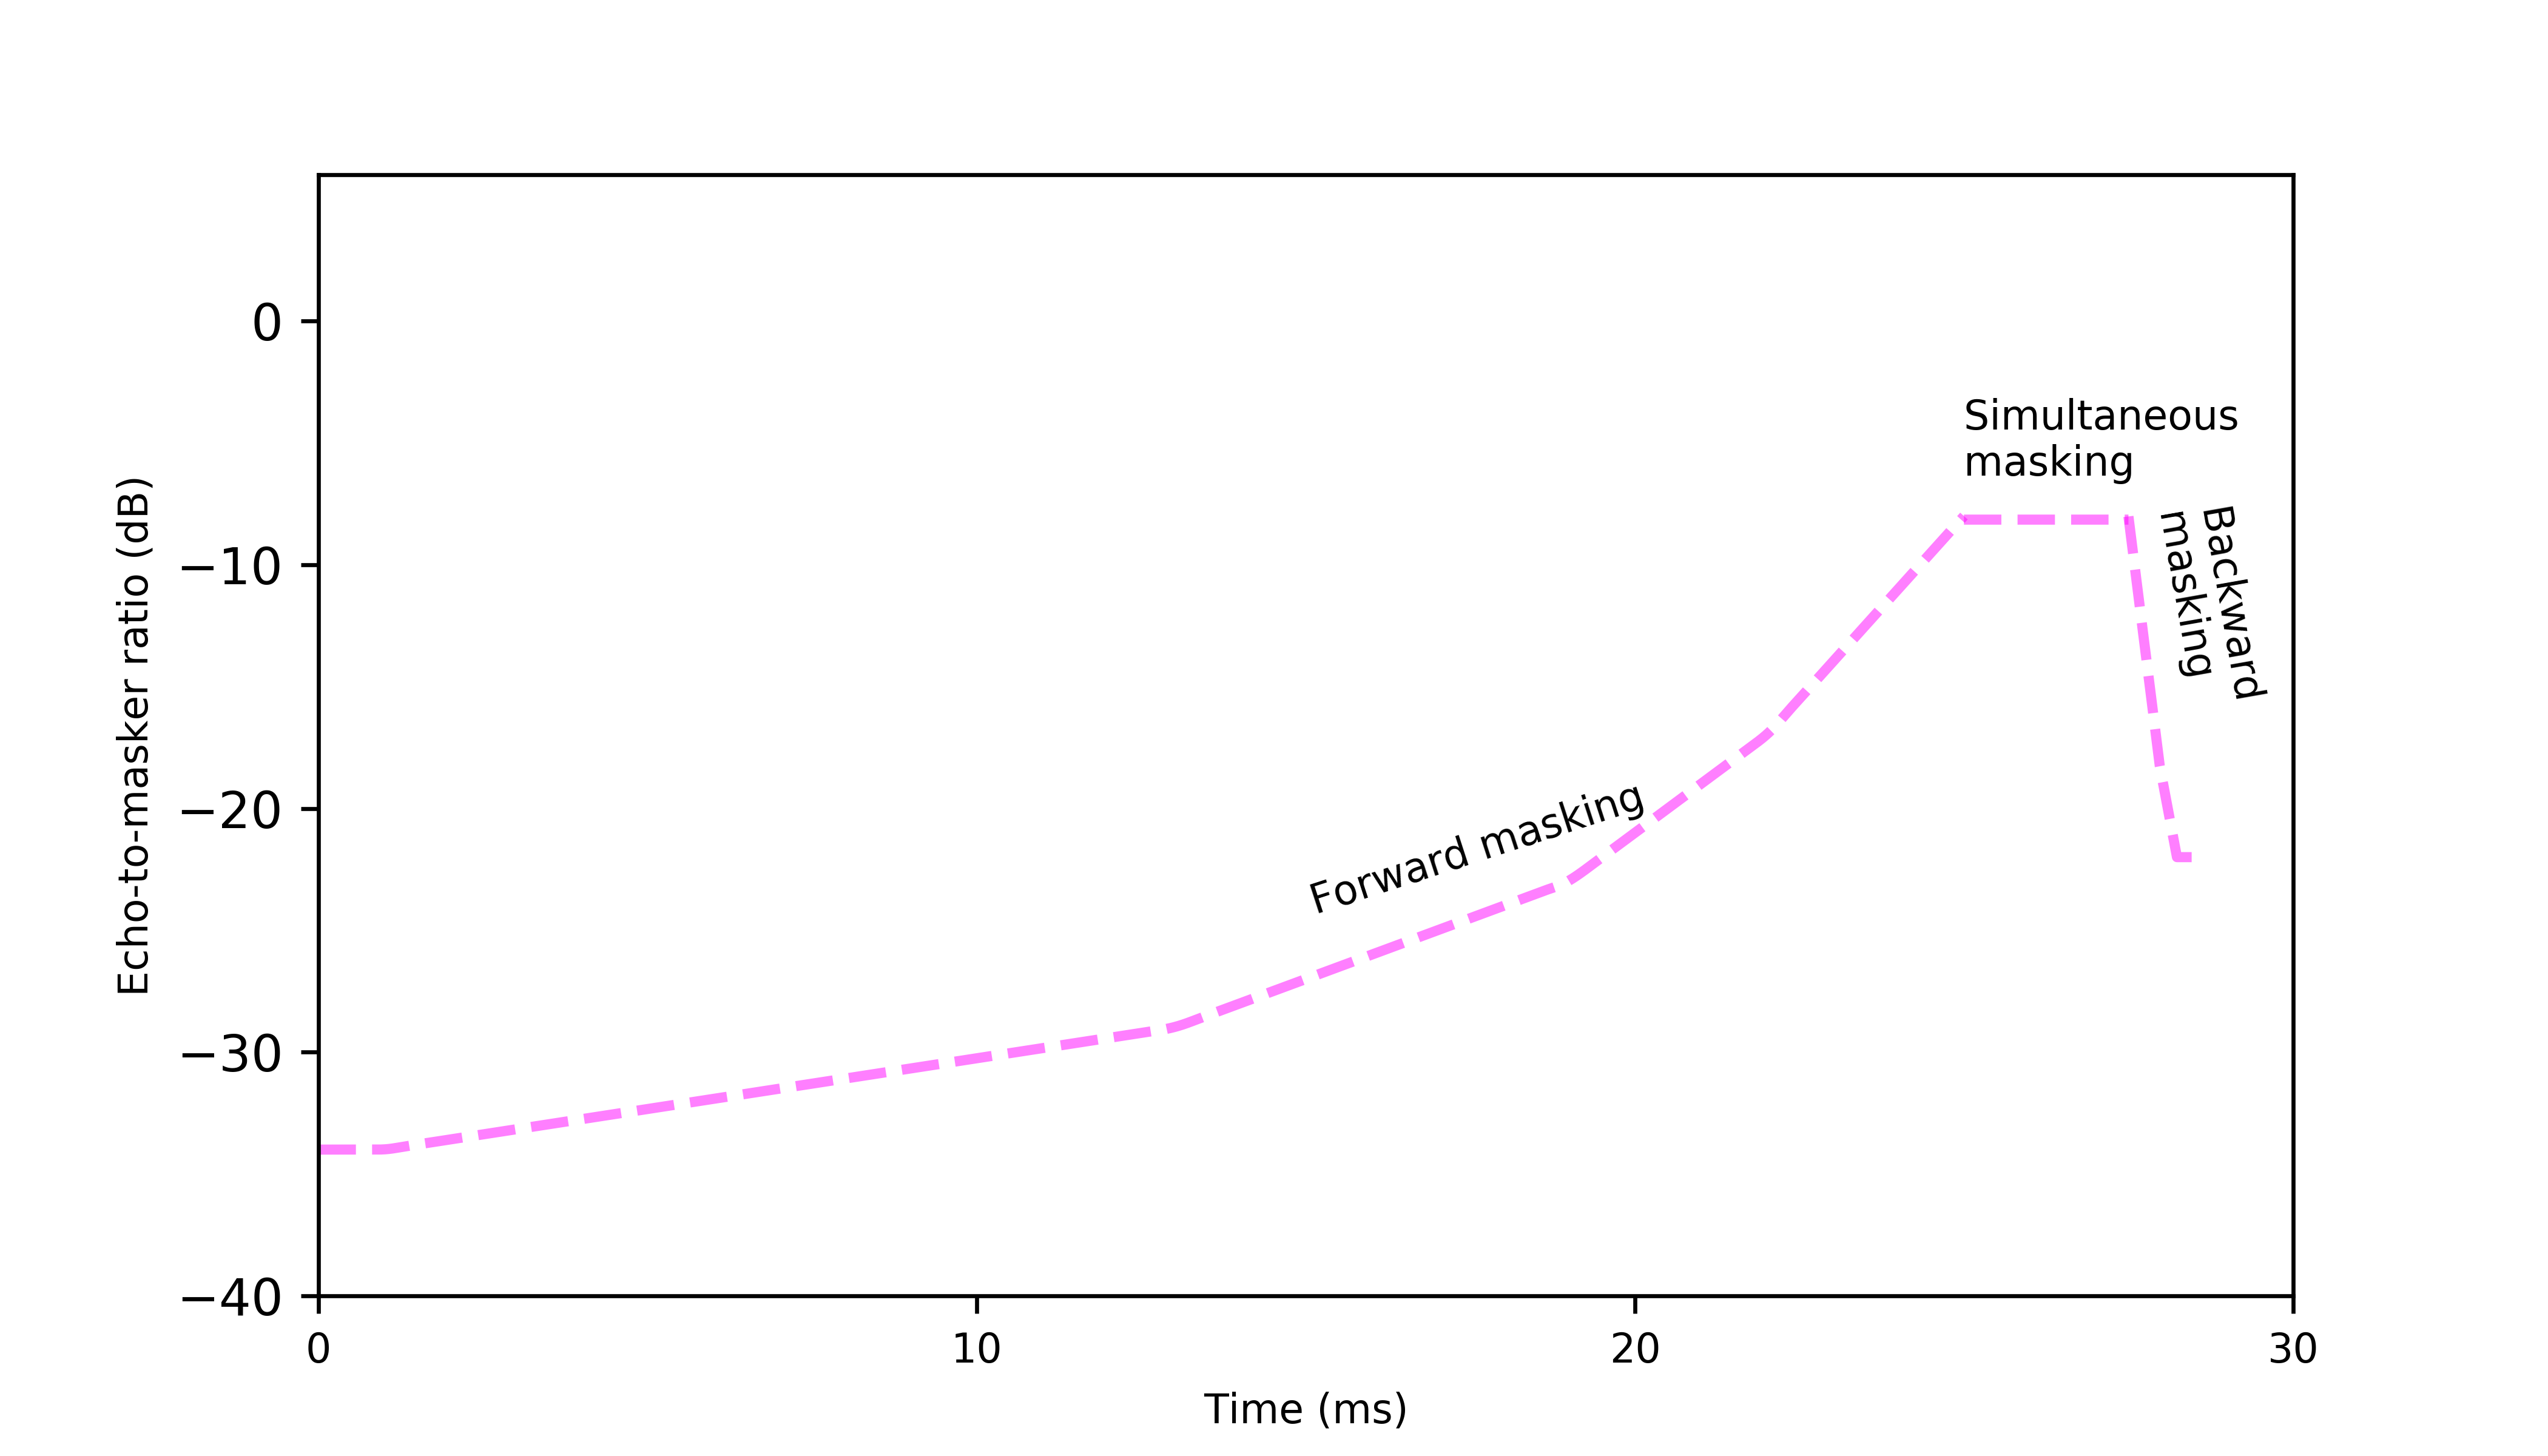
\includegraphics[]{original_papers/CPN_figures/Figures_SI/Figure_S1.png}
\centering
\caption{ The 'temporal masking envelope' used to simulate temporal masking. The envelope represents the lower echo-to-masker ratios at which a bat can detect echoes for various echo-masker delays. The envelope is the equivalent of the lowest signal-to-noise ratios at which echoes can be detected over different time delays. The envelope is centered on the position of the echo, and has a long forward masking section (at times prior to the echo), and a short backward masking section (at times after the echo). The simultaneous masking region is equal to the length of the echo itself. If the echo-to-masker ratio profile is above the temporal masking envelope for most of its duration (i.e., the echo-to-masker SPL ratio was higher than required for echo detection), we considered an echo to be heard. If the echo-to-masker ratio profile is below the envelope for more than 25$\%$ of the echo's duration, the echo was considered not heard. Here the temporal masking envelope is shown for a 2.5 ms echo. Data and sources used to construct the temporal masking envelope are given in Table 2.2}
\label{cpn_figS1}
\end{figure}

\newpage

\begin{figure}
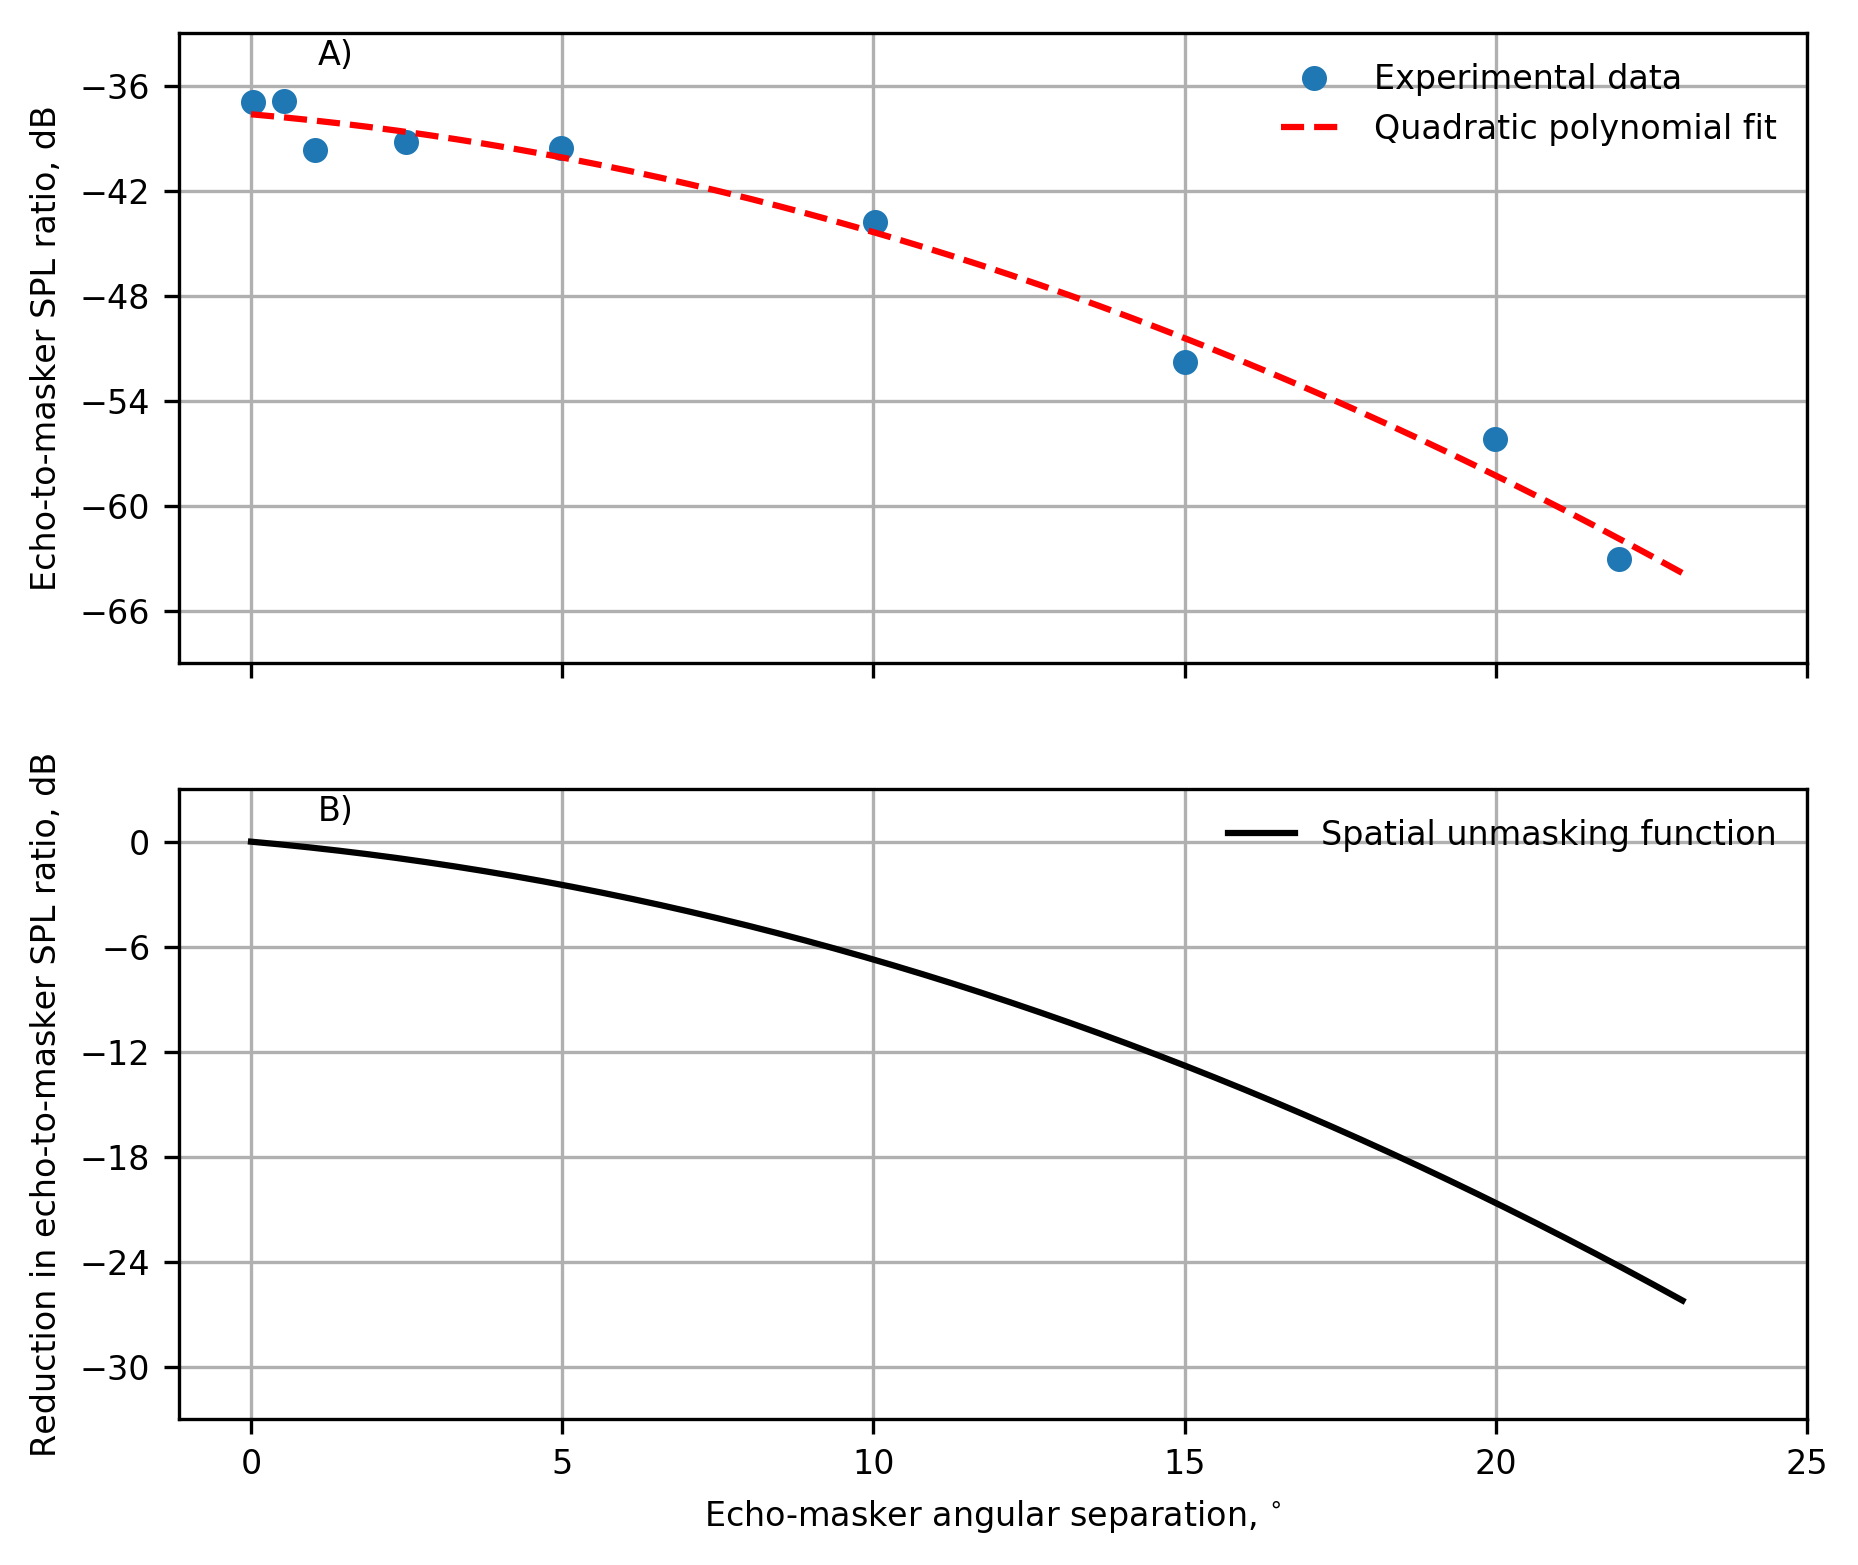
\includegraphics[]{original_papers/CPN_figures/Figures_SI/Figure_S2_2panel_exptldata_on_top.png}
\centering
\caption{The ‘spatial unmasking function’ describes the reduction in echo-to-masker SPL ratio at echo detection as a function of angular separation between echo and masker. A) The original data set of \cite{suemer2009a} (blue dot) and our digitized and
interpolated dataset (red line). The error between the data and our interpolation is less than 2 dB. B) The final spatial unmasking function as used in our simulations was derived from the interpolated fit in A), which was normalised to the echo-to-masker ratio at zero degrees angular separation. This final spatial unmasking function describes the reduction in required echo-to-masker SPL ratio relative to the co-localized case: when echo and masker are co-localized, the reduction is 0 dB, while the reduction becomes greater with increasing angular separation.}
\label{cpn_figS2}
\end{figure}

\newpage

\begin{figure}
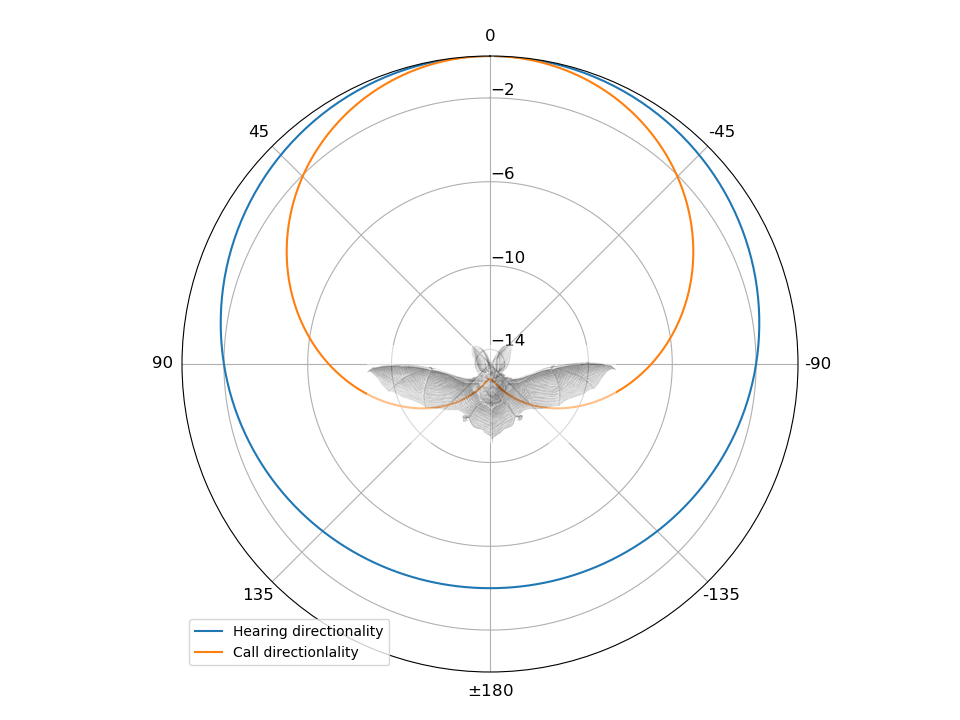
\includegraphics[]{original_papers/CPN_figures/Figures_SI/Figure_S3.png}
\centering
\caption{Calling and hearing directionality of bats. Call directionality (orange) is directional, with a difference of up to -14 dB in source level from front to back. Calls emitted to the front of a bat result in higher received levels of calls, echoes and secondary echoes. Hearing directionality (blue) is less directional, with a difference of up to -4 dB from front to back. Hearing directionality causes sounds arriving from the back to be perceived fainter than sounds arriving from the front. Bat drawing from Kunstformen der Natur (Ernst Haeckel, 1899).}
\label{cpn_figS3}
\end{figure}

\newpage

\begin{figure}
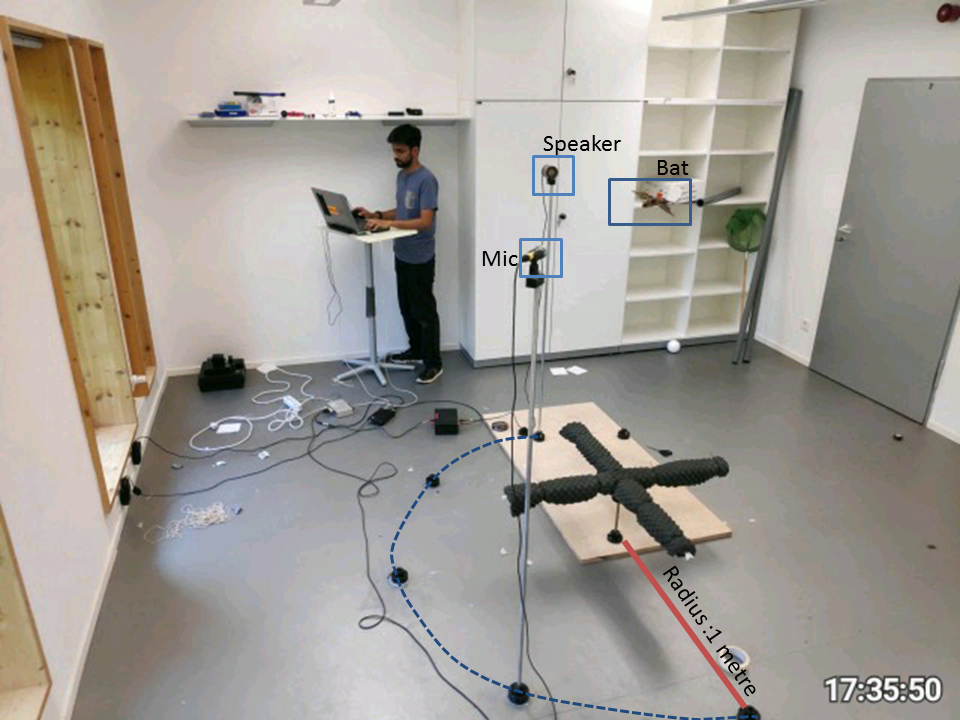
\includegraphics[]{original_papers/CPN_figures/Figures_SI/Figure_S4.png}
\centering
\caption{The ensonification setup used to measure the monostatic and bistatic target strength of a bat as an acoustic target. A stuffed \textit{Myotis myotis} bat was hung at the same height as the speaker and microphone. The bat could be rotated in the azimuth. The microphone and speaker were placed at 1 m radius around the bat at various positions (black rounded plastic molds on floor) with a separation of 45° from each other. By a combination of bat orientation, microphone and speaker positions all possible incoming and outgoing relative angles were measured. Here the positions of the speaker and microphone for a bistatic target strength measurement with 135° angle between microphone and speaker are shown.}
\label{cpn_figS4}
\end{figure}

\newpage

\begin{figure}
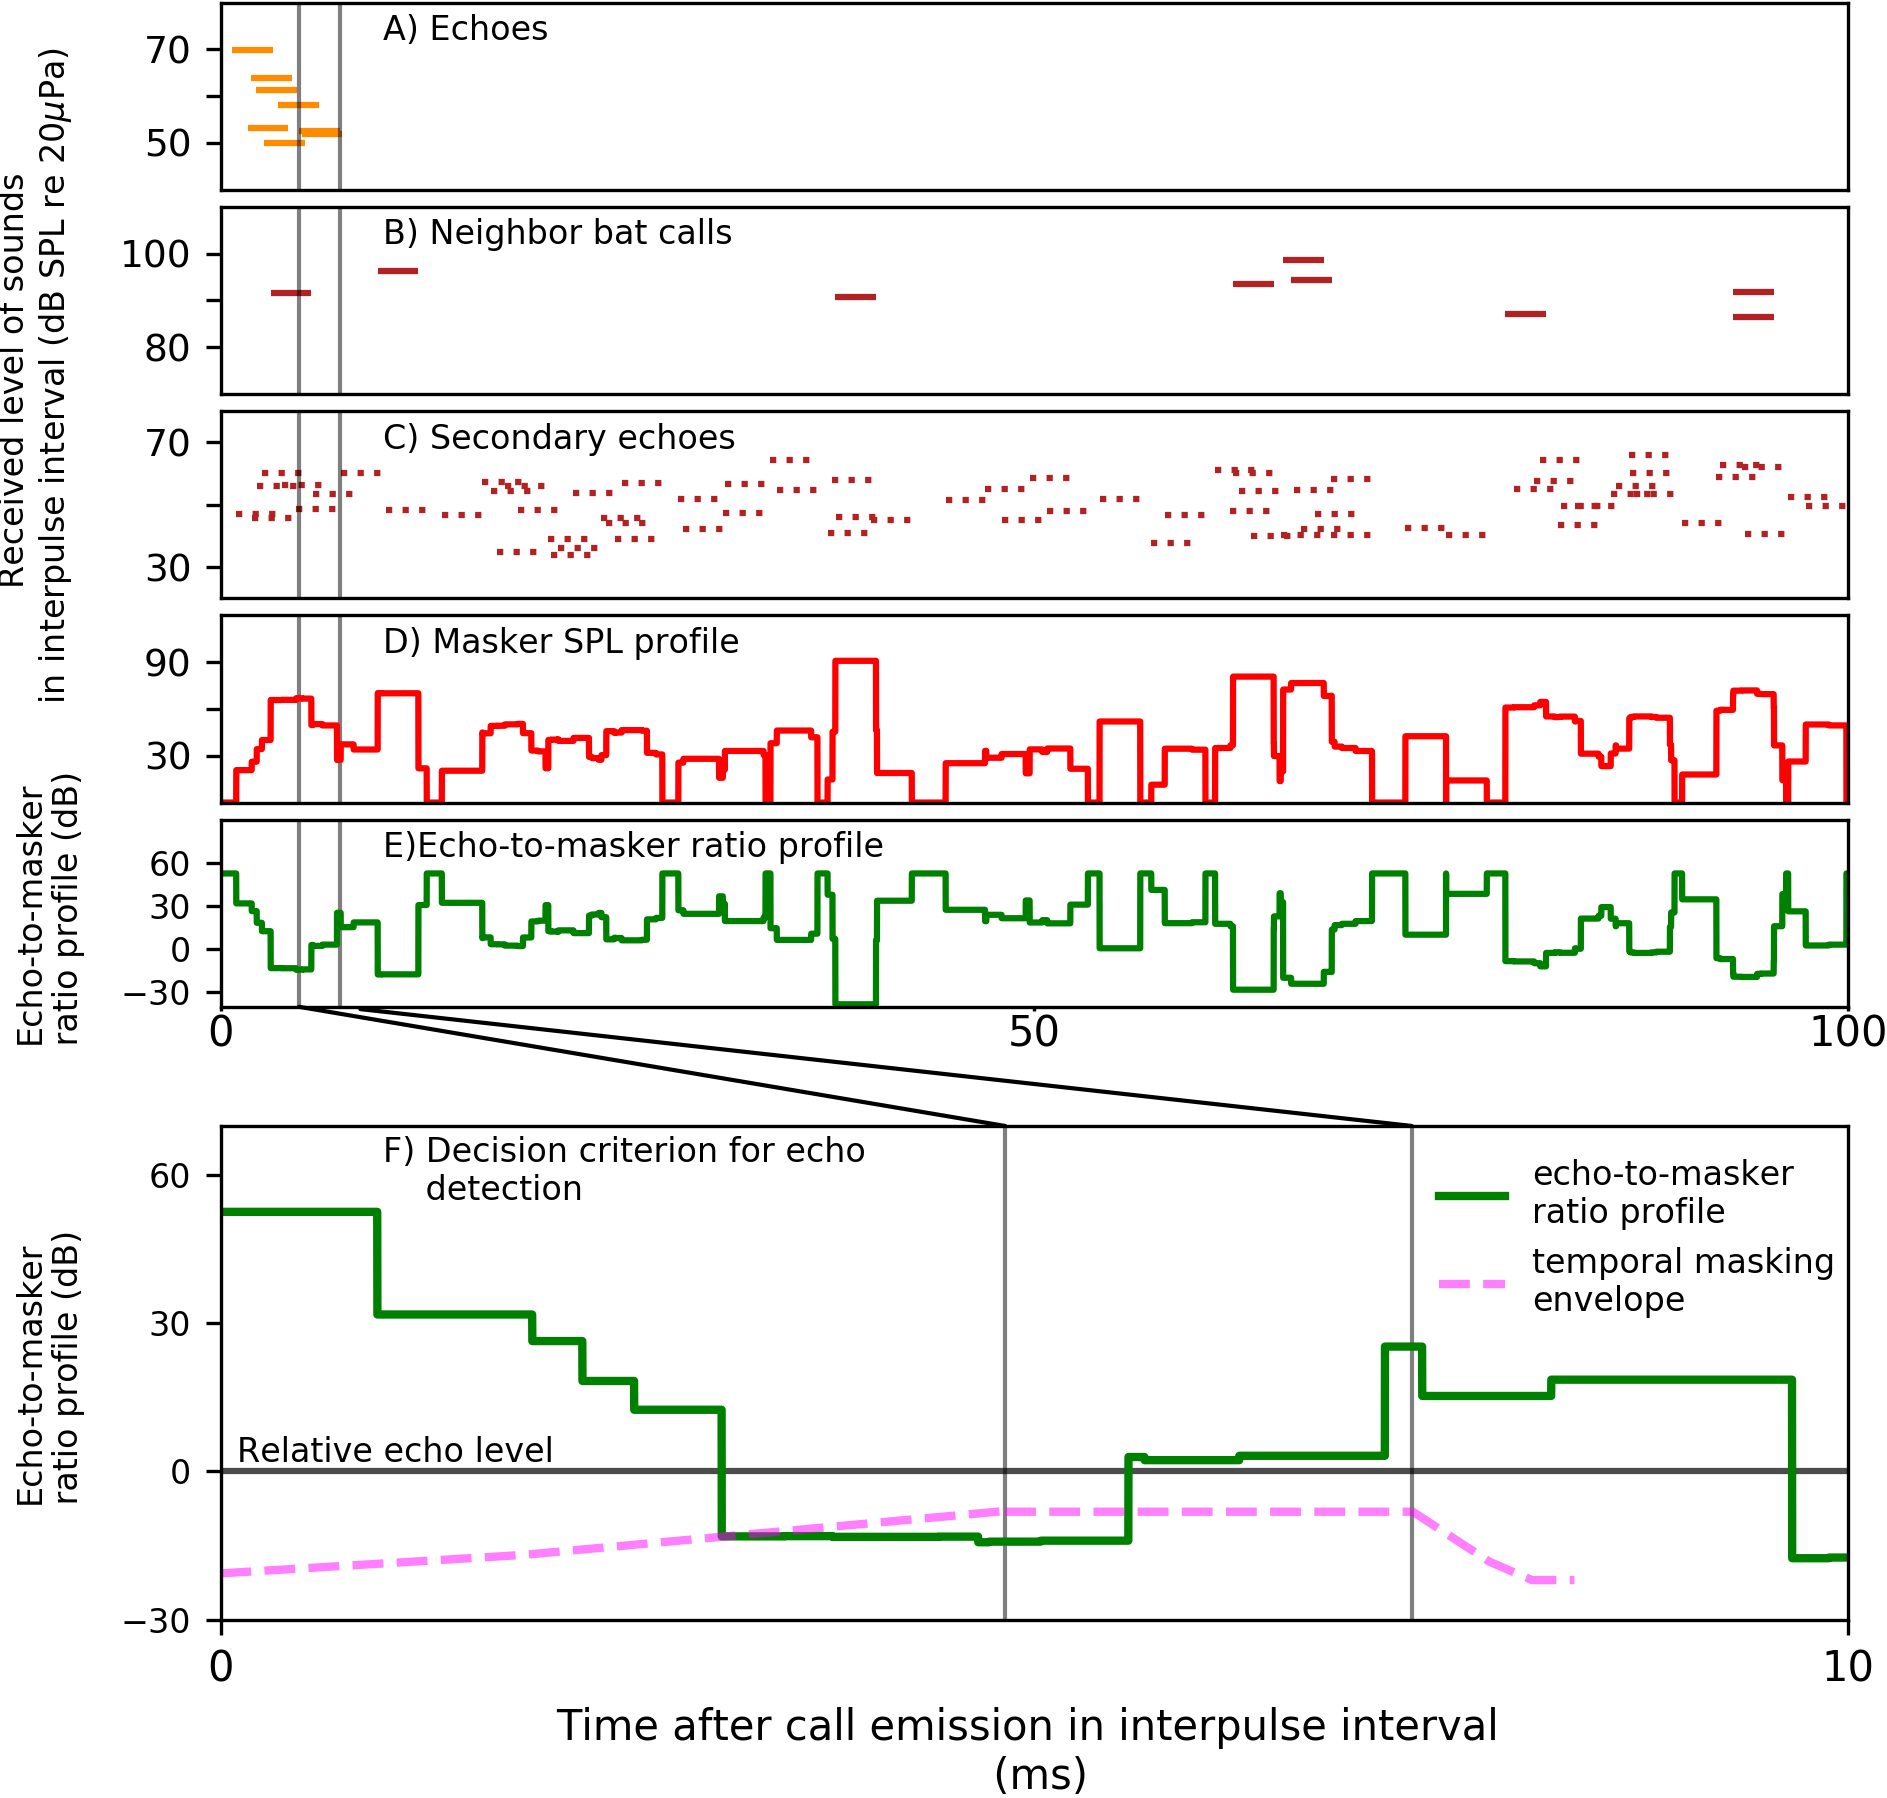
\includegraphics[]{original_papers/CPN_figures/Figures_SI/Figure_S5.png}
\centering
\caption[caption1]{Schematic representation of the sounds arriving in the interpulse interval for a simulation with a group of 10 bats (A-C) and how echo detection was determined (D-F). A-E show the full interpulse interval of 100 ms, while F shows an enlargement of the first 10 ms.  A) Timing and received SPL of the individual echoes reflected off neighbors. The echoes arrive at delays corresponding to the neighbors’ distance from the focal bat. The vertical lines single out one specific target echo to illustrate the simulated auditory system (see F). B) Timing and received SPL of the calls from neighboring bats arriving randomly with a uniform probability over the interpulse interval. C) Timing and received SPL of the secondary echoes in the interpulse interval, arriving randomly with uniform probability over the interpulse interval. D) The masker SPL profile obtained by adding the effective masker SPL of all maskers (calls and secondary echoes) over time for the chosen echo. The effective masker SPL is the received SPL corrected for spatial unmasking based on the angular separation between the echo and the masker, using the spatial unmasking function in Figure \ref{cpn_figS2}. E) The echo-to-masker ratio profile obtained by normalizing the echo SPL to the masker SPL profile. 0 dB is the echo's relative SPL. F) Determining whether an echo was heard or not, by comparing the echo-to-masker ratio profile (solid green) to the temporal masking envelope (dashed pink). If the echo-to-masker ratio is above the temporal masking envelope, then the echo was not masked. In contrast, if the echo-to-masker ratio is cumulatively below the temporal masking envelope for more than 25$\%$ of the echo's duration (of 1 or 2.5 ms), then the echo was considered masked. The vertical lines indicate the actual temporal location of the example echo from A). The temporal masking envelope is centered on the chosen echo. Here, the echo-to-masker ratio is below the temporal masking envelope for almost a whole echo duration, meaning that this echo was masked.
}
\label{cpn_figS5}
\end{figure}

\hypertarget{hbcchapter}{%
\chapter{High duty-cycle bats in the field do not alter echolocation calls when flying in groups}\label{hbcchapter}}

\chaptermark{group echolocation in CF-FM bats}

This chapter is a manuscript under preparation:

\emph{Neetash M. Rajagopalachari\(^{*}\), Thejasvi Beleyur\(^{*}\), Aditya Krishna, Holger R Goerlitz, (2021) High duty-cycle bats in the field do not alter echolocation calls when flying in groups}

\emph{\(^{*}\): joint first authors}

\newpage

\hypertarget{hbcabstract}{%
\section*{Abstract}\label{hbcabstract}}
\addcontentsline{toc}{section}{Abstract}

Groups provide benefits to their members, but also challenge individual sensory systems. Roosting sites and leks for instance are filled with a multitude of signals, of varying relevance to each individual. Studies to date have looked at groups of passive sensing animals that act as receivers of sensory stimuli. Each individual in a passive sensing group detects its surroundings without majorly affecting the sensory systems of their neighbours. Active sensing animals in contrast emit probes of energy to detect their surroundings. Echolocating bats emit intense calls and listen for returning echoes to perceive their environment. When echolocating in groups, bats may not be able to detect their own echoes due to masking by the intense calls of their neighbours. Bats use a variety of sensory strategies to cope with such acoustically challenging conditions. To date however, most studies have been performed on low duty-cycle bats that emit short frequency-modulated calls with long pauses. In contrast, high duty-cycle bats that emit long calls with short pauses are understudied despite their higher chances of call-echo overlap during group echolocation. Studying high duty-cycle bats has also been hindered by a lack of methods to analyse overlapping calls. We developed methods to analyse and extract call parameters of temporally overlapping calls and studied the echolocation of multiple free-flying high-duty cycle bats of the genus Rhinolophus in the field. Our results show that bats did not do not seem to alter their call parameters even when flying in groups (with up to 4 other individuals). This lack of response is in contradiction to a previous flightroom study. Our results highlight the robustness of bat echolocation, and the importance of studying behaviour under natural conditions.

\newpage

\hypertarget{introduction-1}{%
\section{Introduction}\label{introduction-1}}

Living in groups provides both costs and benefits to the group members, which individuals have to balance \citep{pulliam1984living}. Advantages of being in a group might be increased foraging success, offspring survival, or thermoregulation, while challenges might include increased parasitism, and competition. An individual's sensory perception is also challenged in groups, due to the multitude of dynamic sensory information from group members, for example in leks, roosting sites, or even at human gatherings. Only a small fraction of this information is relevant to a receiver \citep{socialintegr}, which necessitates various adaptations to filter out irrelevant information, including unique calls (e.g., mate contact calls in penguins) or avoiding signal overlap with neighbours (e.g., in frogs and cricket pairs) \citep{socialintegr}.

Many studies to date have focused on sensory filtering in passive sensing animals, i.e., animals that sense their surroundings by receiving external energy (e.g., penguins, frogs, humans)\citep{zweifel2020defining, nelson2006a}. As each passively-sensing group member receives external information independently, their sensory processes do not affect other individuals around them. In contrast, active sensing animals like electrolocating fish or echolocating bats face a unique sensory challenge when actively sensing in social groups {[}\citet{ulanovsky2008bat};\citet{gillambrasiliensis};\citet{watanabe1963change}). Echolocating bats emit intense ultrasonic calls and detect their surroundings by listening for the echoes reflecting off objects around them \citep{griffin1958listening}. In groups however, a bat's returning echoes can be overlapped by the calls and echoes from its neighbours, preventing detection of its surroundings\citep{ulanovsky2008bat}. Active sensing animals thus face the issue that their information of interest is potentially masked by the multitude of surrounding signals in a group. An echolocating bat in a group may thus end up metaphorically flying `blind', as without detecting its own echoes it cannot sense its environment.

A combination of laboratory and field studies have shown the diverse behavioural responses of bats in response to sensory challenge from groups and experimental playbacks. Bats increase call levels, alter temporal features such as call rate, duration and duty cycle \citep{amichai2015calling, jarvis2013groups, lu2020echolocating, hage2013ambient, lin2016a, gomes2020individual}, and spectral properties such as bandwidth and terminal frequency \citep{hase2018bats, cvikel2015b, gotze2016no, fawcett2015echolocation}. These responses however are not uniform across species, with different species showing seemingly opposite responses to similar situations \citep{ulanovsky2004dynamics, amichai2015calling, jarvis2013groups, adams2017suppression}.

There are two broad groups of echolocating bats \citep{fenton2012evolution} characterised by their duty cycle, i.e., the fraction of time spent emitting calls. The first and major group of bats are low-duty cycle bats. They typically emit frequency-modulated (FM) calls. The second group are high-duty cycle bats which typically emit calls with a long constant-frequency (CF) component and one or two flanking short FM components (CF-FM calls). In contrast to low-duty cycle bats, the calls of high-duty cycle bats are longer (10 to \(\geq\) 50ms) and thus have higher duty cycles of \textasciitilde30-60\(\%\) \citep{fenton2012evolution}. Higher duty cycle directly increases the probability of temporal overlap and thus masking of echoes by calls \citep{beleyur2019modeling}. High-duty cycle bats such as rhinolophids and hipposiderids are thus likely to be more affected in group echolocation than low-duty cycle bats, making them a unique system to understand the sensory strategies echolocators use in challenging conditions. Most studies on group echolocation so far investigated low-duty cycle bats \citep{lin2016a, fawcett2015clutter, gotze2016no}, likely due their speciosity (\textasciitilde87\% of all echolocating bats \citep{fenton2012evolution, mammdivdatabase} and ease of call analysis. A wider variety of species need to be studied, to understand the echolocation responses in context of their ecology and auditory systems.

A typical CF-FM call has of up to three call components: a short initial upwards FM sweep (iFM), a long central CF segment (CF), and a short terminal downward FM sweep (tFM) (sensu \citet{tian1997echolocation}). The CF component is used for the flutter detection of prey wingbeats \citep{schnitzler2011auditory} based on high-resolution frequency analysis around the CF frequency in the bat's auditory fovea \citep{neuweiler2000biology}. Different species and even individuals within a species use different CF-frequencies that are matched to the frequency tuning of their acoustic foveas \citep{schnitzler1976peripheral}. Individual bats also compensate for flight-induced Doppler shifts to keep the CF-frequency of the returning echo within their acoustic fovea \citep{schnitzler1973control, schoeppler2018precise}. Despite potential temporal overlap of emitted call and returning echo, Doppler-shift compensation spectrally separates the CF parts of the echo and call when a bat is echolocating alone. In groups however, temporal and spectral overlaps between neighbours' calls and own incoming echoes is bound to occur. While the CF component is involved in prey detection, the tFM component is thought to be involved in target ranging \citep{tian1997echolocation, neuweiler1987foraging}, and the role of the iFM remains ambiguous. Comparable to call alterations in FM-bats \citep{Fenton2014}, CF-FM bats show rapid alterations in tFM bandwidth and duration based on the behavioural context, e.g.~resting, landing or prey capture \citep{neuweiler1987foraging, schoeppler2018precise, tian1997echolocation}.

Previous investigations of group echolocation in CF-FM bats found no support for changes in CF frequencies to avoid spectral overlap (``jamming avoidance response'')\citep{jones1993echolocation, jones1994individual, fawcett2015echolocation}. Recent studies in low duty cycle FM bats also questioned the efficacy of a jamming avoidance response in groups \citep{gotze2016no, cvikel2015b, mazar2020sensorimotor}. In contrast to the CF-component, we are only aware of one study that quantified changes of the FM-component in group flight, reporting an increased tFM duration and bandwidth \citep{fawcett2015echolocation}. Given the tFM's flexibility and role in ranging, there is a strong need for its explicit quantification in multi-bat contexts. The tFM may show the same kinds of changes in multi-bat contexts as shown in low-duty cycle bats, which also use their FM calls primarily for ranging \citep{fawcett2015clutter, amichai2015calling, hase2018bats}.

Studying group echolocation in high-duty cycle bats entails analysing audio with overlapping calls. The analysis of recordings with overlapping calls is a nascent field (but see \citet{izadi2019segmentation}), and acoustic measurements have not been attempted to the best of our knowledge . Even studies with multiple high-duty cycle bats have been limited to 2-3 bats in flightroom conditions \citep{fawcett2015echolocation, jones1993echolocation, jones1994individual}. Here, we developed methods to extract echolocation parameters in the presence of overlapping calls and to investigate the high-duty-cycle echolocation of group-flying horseshoe bats in a natural cave.

\hypertarget{methods}{%
\section{Methods}\label{methods}}

\hypertarget{study-species-and-site}{%
\subsection{Study species and site}\label{study-species-and-site}}

Two species of rhinolophid bats Rhinolophus mehelyi and R. euryale were recorded in their natural environment. Both species emit CF-FM calls with peak frequencies between 102-112 kHz, and are not acoustically distinguishable due to overlap in their call characteristics \citep{dietz2016bats}. For the purposes of this study, we thus treated them as a single group of bats that may face the problem of acoustic jamming due to the similarity in spectro-temporal call structure.

We observed bats that flew in an out of and rested inside a small dome-shaped cave (Figure \ref{fig:cavesetupschematic}) next to the main entrance of the Orlova Chuka cave system, Bulgaria. The cave had a size of approximately 5 x 3 x 1.6 m\(^{3}\) (l x b x h), one opening where bats flew in and out of throughout the night, and some roosting sites on the inside.

\hypertarget{experimental-setup}{%
\subsection{Experimental setup}\label{experimental-setup}}

We placed an experimental audio-video setup inside the cave, consisting of three microphones and two infrared cameras. Two consumer grade CCTV cameras (UVAHDBP716) with infrared lamps were connected to a digital video recorder (XVR1004) to record the flight of bats as they flew in and out of the cave. The system recorded video
mostly at 22 Hz, however there was frame rate variation between 18-27 Hz. Video feeds were time-synchronised (but not frame-synchronised) by common burnt-in time stamps on the frame. The two cameras were placed in approximately the same position on every recording night. The cameras were placed to maximise the total cave volume recorded
while also capturing the blinking LED light. Video was recorded continuously through the night. Audio from three CM16 microphones (Avisoft Bioacoustics, Glienicke, Germany) were recorded by a 416H soundcard (Avisoft Bioacoustics, 250 kHz sampling rate, 16 bit resolution). As horseshoe bat calls are directional \citep{matsuta2013adaptive}, the three microphones were placed at different positions in the cave to increase the number of on-axis calls captured (Figure \ref{fig:cavesetupschematic}). Microphones were placed in the same location with an estimated +/- 10cm error in the cave across multiple nights. Audio was recorded continuously through the night as consecutive multichannel files of 1 minute duration.

The audio and video feeds were synchronised using the method described in Laurijssen et al.~2018. In short, ON-OFF signals with variable durations between 0.08-0.5 s were generated by a portable computer (Raspberry Pi 3) and recorded on the audio soundcard and used to drive the blinking of an LED that was recorded by the two cameras. (See Supplementary Information (SI) \ref{avmatching} for signal generation script, electronic circuit and
associated notes).

\begin{figure}
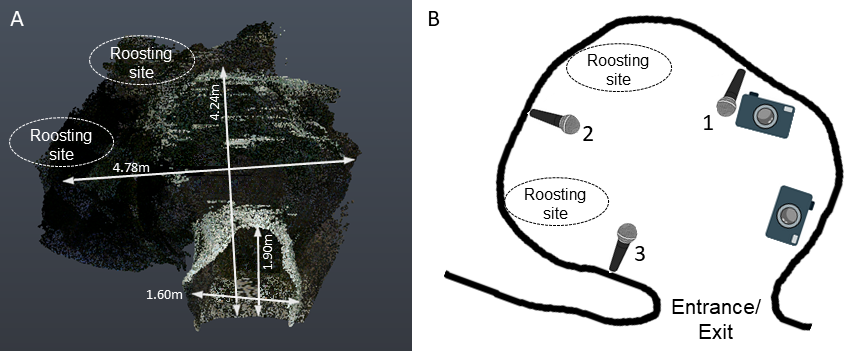
\includegraphics[width=1\linewidth]{original_papers/hbc-paper/figures/pointcloud_and_topview} \caption{\label{cavesetupschematic}Point cloud scan (A) and schematic of the cave, indicating the entrance/exit, the typical roosting sites inside the cave, and the position of microphones and cameras.   (3D scanning by Klaus Hochradel, UMIT Tirol) The numbers next to the microphone correspond to the positions in the main text.}\label{fig:cavesetupschematic}
\end{figure}

\hypertarget{video-analysis-to-determine-group-sizes}{%
\subsection{Video analysis to determine group sizes}\label{video-analysis-to-determine-group-sizes}}

Bat activity in the cave was recorded for a total of about 12 hours across four nights (16-19 August 2018). After entering the cave, bats typically flew around for a few seconds or flew to the roosting site, where they stayed for several seconds to minutes, and later exited from the cave again. We watched the videos and manually identified bat flight activity, noting its start and end time and the number of visible bats. A bat flight activity is defined as the interval during which the number of visible bats flying inside the cave is constant.
Successive bat flight activities were operationally defined as being separated from one another by least 6 frames (\textasciitilde0.3 s). We defined the start of bat activity as the frame a bat was observed to fly in either of the two camera view. Similarly, the end of bat flight activity was when a bat was not observed anymore in either of the camera views. Multi-bat contexts could have dynamic transitions in the number of bats, and we annotated the start
and end of the multi-bat activity with the part of the video that had the maximum number of bats (See SI 0.2 for more details).

\hypertarget{synchronsing-bat-flight-activity-in-video-and-audio}{%
\subsection{Synchronsing bat flight activity in video and audio}\label{synchronsing-bat-flight-activity-in-video-and-audio}}

For each bat flight activity identified in the video, we identified the corresponding region of the recorded audio. The synchronization signal in the video was quantified by quantifying the median intensity of the pixels in the region around the LED. We then cross-correlated the normalized normalized pixel intensity with the recorded ON/OFF voltage signal in the audio. We managed to successfully find audio matches for 1181 video annotations (55\% of 2132 video annotations). The low match rate is primarily due to the fluctuating camera frame rates, and because many of the matched audio files originated from non-target bat species, which could not be discriminated from our target speices \emph{R. mehelyi/euryale} while annotating the videos. Observed non-target species were \emph{R. ferrumequinum} and vespertilionid and miniopterid FM bats, all of which occur in the Orlova Chuka cave system \citep{ivanova2005important}. For the acoustic analysis we chose matched audio files that only had \emph{R. euryale} and/or \emph{R. meheyli} calls.

\hypertarget{acoustic-parameter-analysis}{%
\section{Acoustic parameter analysis}\label{acoustic-parameter-analysis}}

All flight activity matched audio files (henceforth referred to as flight-activity audio) were first forward-backward high-pass filtered at 70 kHz (2nd order Butterworth filter). For the analysis we used recordings from the first microphone, as it appeared to have consistently captured calls with the least reverberance of the three channels. The first microphone was located facing the cave opening, perhaps therefore capturing calls of both entering and exiting bats well.

We quantified frequency, duration and amplitude of the three parts components of the echolocation call (iFM, CF and tFM) using two complementary acoustic analyses. The first analysis is the `individual call' analysis, where we measured parameters of one individual echolocation call from each flight activity audio file. The second analysis is the `window' analysis. Each flight-activity audio was split into consecutive windows of 50 ms duration. We then measured the acoustic parameters per window of all windows of a flight-activity audio. In recordings with multiple bats, the 50 ms windows could contain overlapping calls.

The advantage of the individual call analysis is that the measurements made on the calls are directly interpretable as call component alterations reveal the sensory decisions of the bats. On the other hand, the disadvantage of the individual call analysis is that especially in multi-bat recordings, it can be difficult to find a non-overlapped call. The window analysis complements individual call analysis by enabling measurements even on audio with overlapping calls. Window analysis also allows a kind of null-hypothesis testing where the observed multi-bat audio can be compared with 1) single bat audio and 2) `virtual' multi-bat audio files created by adding multiple single bat audio files. These `virtual' multi-bat audio files recreate a scenario where two bats echolocate in the same volume without actively responding to each other's presence. The disadvantage with window analysis is the lack of call-level measurements. Ultimately, using the two approaches simultaneously strengthens the interpretation of our results.

\hypertarget{individual-call-analysis}{%
\subsubsection{Individual call analysis}\label{individual-call-analysis}}

Per flight activity audio, we chose one call that was not overlapped by other calls and that had a signal-to-noise ratio of at least 20 dB (Figure \ref{fig:itsFMdemo}) through a random search protocol (SI \ref{indcallprotocol}). Briefly, from a randomly determined time point, an experimenter began searching into a randomly determined direction (backward or forward in time) until a suitable horseshoebat call was found. We were able to find 226 individual calls across all the synchronised audio files. Calls were automatically segmented into their corresponding parts iFM, tFM or CF (Figure \ref{fig:itsFMdemo}) ) using the itsfm package \citep{itsfmcitation}. Most approaches to date focus on segmenting CF-FM calls into their components by high/low pass filtering around the peak frequency of the call \citep{siemers2005species, schuchmann2012horseshoe, tian1997echolocation, lu2020echolocating, schoeppler2018precise}. For an accurate estimate of the peak frequency, this approach requires a recording of the call with a prominent CF component. While suitable for laboratory studies, filtering around the peak frequency fails in the analysis of CF-FM calls recorded in the field under a variety of conditions eg. calls with loud FM and faint CF components. \emph{itsfm} overcomes these limitations by tracking the change in frequency over the call time to segment it into FM and CF components.

From the segmented CF and FM components we measured specific parameters. In the CF component, we measured the peak frequency, RMS level and duration. The CF peak frequency was quantified as because bats may shift their CF frequencies in the presence of conspecifics. From the FM components, we measured the lower frequency (-10 dB peak frequency of the FM audio segment), bandwidth (defined as difference between the CF peak frequency and the lower frequency of the FM segment), RMS level and duration. We also calculated the iFM/CF and tFM/CF amplitude ratios, i.e., the relative amplitude of the iFM and tFM component relative to the CF component. The relative call component measures were calculated as CF-FM bats are known to independently vary the level of call components in a context specific manner (Tian and Schnitzler 1997; Lu, Zhang, and Luo 2020).

\begin{figure}
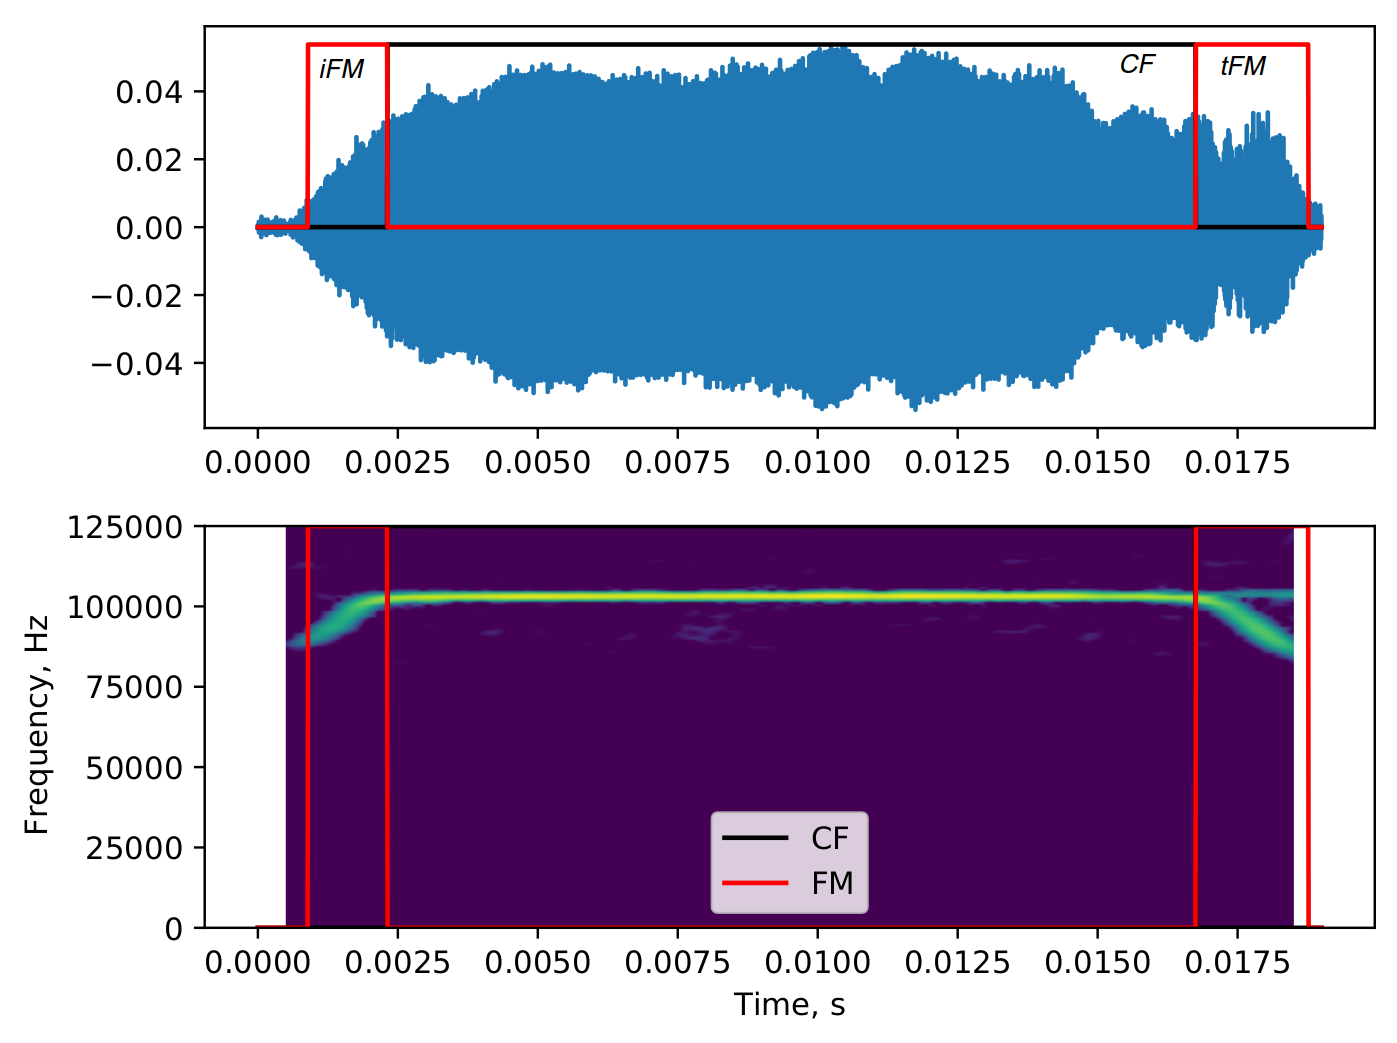
\includegraphics[width=1\linewidth]{original_papers/hbc-paper/figures/fig1_labelled_original_from_20180816_21502300_30} \caption{Example of a manually selected CF-FM call, which was automatically segmented into its initial frequency-modulated (iFM), central constant-frequency (CF) and terminal frequency-modulated (tFM) components based on frequency change over time , using the *itsfm* package. The itsfm package allows accurate segmentation into call components  under challenging recording conditions}\label{fig:itsFMdemo}
\end{figure}

\hypertarget{windowed-calls-analysis}{%
\subsubsection{Windowed calls analysis}\label{windowed-calls-analysis}}

Each flight activity audio was split into consecutive 50 ms windows (See SI \ref{windowdetails} for details of window splitting). We chose a window duration of 50 ms as it provided high spectral resolution (20 Hz at 250 kHz sampling rate) that allows to distinguish between multiple CF components that may be contained in the window. Initial observations showed that 50 ms was about the longest observed duration of a bat call in our data, and was about twice the length of typical calls.

Over the course of a flight activity audio , there may be multiple windows without calls or very faint calls in them. To exclude those windows, we removed all windows whose RMS level were not at least 20 dB above the maximum RMS level of manually annotated audio segments without calls (for details, see SI \ref{silentwindow}). From the remaining windows that contained echolocation calls, we measured each window's received RMS level, dominant frequencies and FM lower frequencies. Dominant frequencies are defined as local frequency peaks in the smoothed power spectrum that are within 14 dB of the window's peak frequency (i.e., the frequency with highest energy in the spectrum). Dominant frequencies are a measurement of the CF frequencies of multiple calls in the same window (for details of dominant frequency measurement see SI \ref{domfreqdetails}). FM lower frequencies were determined by a spectrogram- based method which identified FM regions and chose the lowest frequency in all FM regions identified in a window (SI \ref{lowestfreqdetails}). There could be multiple terminal and dominant frequency values for a single window, however only one received RMS level measurement per window. We chose the measurements in the window analysis to be analogous to the measurements in the individual call analyses: the dominant frequencies in the window analysis complements the CF peak frequency measurements in the individual call analysis, while the lower frequencies and RMS measurements of the FM parts are analogous to the bandwidth and RMS level of the FM parts of the individual call analysis.

The advantage of the window analysis is the possibility to make `virtual multi-bat' data \citep{fawcett2015echolocation, ratcliffe2004conspecifics} by combining observed single bat call measurements or sequences. We created virtual multi-bat audio by combining single bat audio-files that were of similar durations (SI \ref{virtualdetails}). This represents a `null' dataset of multiple bats that were echolocating, but not responding to each other's presence. We performed the same window acoustic analysis on the virtual multi-bat audio as described above.

\hypertarget{statistical-analysis}{%
\subsection{Statistical analysis}\label{statistical-analysis}}

We observed up to four bats flying in the cave at the same time. Especially in the individual call dataset the number of recordings of multi-bat (\(\geq\) 2 bats) calls was low (N=177, 40, 7, 2 for group sizes of 1, 2, 3, 4 respectively,), we thus combined all annotations with \(\geq\) 2 bats into a multi-bat class and compared `single' and `multi' bat calls in the individual call analysis. To maintain consistency with individual call analysis we also performed comparisons of `single-bat', `multi-bat' and `virtual-multi-bat' flight-activity audio in the window analysis.

\hypertarget{indcallstatanalysis}{%
\subsubsection{Individual call analysis}\label{indcallstatanalysis}}

We calculated the median difference between multi-bat and single- bat conditions (\(median_{multi}-median_{single}\)) for all parameters except CF peak frequency. For CF peak frequencies, we calculated the range difference (\(Range_{multi}-Range_{single}\)) of CF peak frequencies in multi bat and single calls. The range difference was calculated because the supposed spectral jamming avoidance response, i.e., a shift in the used call frequencies, leads to an increased frequency range \citep{habersetzer1981adaptive}, or, as paradoxically has also been observed, a narrower range \citep{furusawa2012convergence}. We performed permutation tests to assess the significance of the observed differences between single and multi-bat conditions.

Our dataset consists of calls from a population of resident wild bats of unknown group size. The same bats may have visited the cave site multiple times over the course of a night. Additionally, bat activity was relatively clustered in time, with median time intervals between consecutive flight annotations of 36 s and 54 s, for annotations used in individual call and window analysis, respectively. Thus, our dataset originates from an unknown number of individuals with an unknown amount of pseudo-replication, potentially lowering the variation in the data. To account for this temporal pseudo-replication, we repeated the analysis by creating two independent subsets from our full dataset: The `clustered' subset contained all calls from the flight activities that were separated by ≤1 min from each other. The `isolated' subset contained all calls from flight activities that ≥1 min from each other. One minute was chosen as it was slightly larger than the observed median inter-annotation interval. Broadly speaking, we expect that if the results of our analysis are comparable across the isolated and clustered subsets, there is a common underlying effect that is independent of temporal clustering. However, if the results of the subset analysis do not corroborate each other, it hints at an effect due to temporal clustering/isolation in the dataset.

\hypertarget{windowed-call-analysis}{%
\subsubsection{Windowed call analysis}\label{windowed-call-analysis}}

In analogy to CF peak frequency range in the individual call analysis, we first calculated the dominant frequency range (\(max_{dominant \: frequency}-min_{dominant \:frequency}\)) across each flight activity audio. We expect variation in the dominant frequency (and thus a non-zero range of dominant frequency) across a flight activity for two reasons: 1) the combined effect of the bat's Doppler shift compensation and 2) the Doppler shift due to the bat's motion relative to the microphone will cause variation in the dominant frequency. These two effects will lead to non-zero dominant frequency range even for single-bat flight activities (SI \ref{simdomfreqranges}). In multi-bat and virtual-multi-bat situations, we expect an increased dominant frequency range due to multiple bats calling at different individual frequencies. We first calculated the median difference in dominant frequency ranges between 1) multi-bat and single-bat and 2) multi-bat and virtual-multi-bat flight activity audio. A permutation test was then performed to assess the significance of the observed median difference.

To understand the theoretically expected dominant frequency range from single and multi bat flights, (and thus the expected range difference) we also performed simulations quantifying Doppler shift and Doppler shift compensation parametrised by the observed data (SI \ref{simdomfreqranges} for details of simulation and results). Briefly we simulated a Doppler-shift compensating bat emitting frequencies between 100-111 kHz, flying past a microphone at various speeds between 1.5-4.5 m/s. The dominant frequency range was calculated as the absolute difference between the frequency recorded by the microphone at the beginning of the flight and the end of the flight. The dominant frequency range estimates from the simulations informed the interpretation of the observed data.

The received level and lowest frequency measurements resulted in multiple values per flight-activity audio (one value per window). The measurements from one flight-activity audio are potentially correlated and we accounted for this potential flight-activity level pseudo-replication by repeated random subsampling followed by median difference calculation. To estimate the median difference between conditions we randomly chose one measurement value per flight activity audio for the single-bat, multi-bat and virtual-multi-bat observations. The median difference between 1) multi-bat and single-bat and 2) multi-bat and virtual multi bat conditions were calculated and followed by the next subsampling round. We performed 10,000 such subsampling iterations, and report the 95-percentile range of median differences in received level and lowest frequency. No tests were run on the median difference estimates obtained for received level and terminal frequency.

To account for temporal pseudo-replication in our study, we also repeated the entire window analysis using clustered and isolated subsets as described in section \ref{indcallstatanalysis}.

\hypertarget{software-packages-used-in-this-paper}{%
\subsection{Software packages used in this paper}\label{software-packages-used-in-this-paper}}

Signal analysis, data manipulation and visualisation were done in Python \citep{van1995python} through its scientific ecosystem: the scipy, numpy, matplotlib, soundfile and pandas packages \citep{2020SciPy, numpy, matplotlib, soundfile, pandas}. Median difference and permutation tests were performed with dabest \citep{ho2019moving} while reproducible analysis, documentation and presentation were enabled by the Jupyter Notebook and Rmarkdown projects\citep{jupyter, rmarkdown}. Audio visualisation, preliminary measurements and single call annotations were done with Audacity \citep{audacity}.

\hypertarget{results-1}{%
\section{Results}\label{results-1}}

We recorded echolocation and flight behaviour of mixed-species groups of the high-duty cycle bats \emph{R. euryale} and \emph{R. mehelyi} as they flew alone and with other bats in a natural cave. The bats performed various flight behaviours in the cave, such as circling, approaches (when two or more bats flew towards each other) and following (one bat behind another) flights. The duration of continuously observed flight bouts varied strongly, ranging from about 0.1 s to 62 s (median: 1.04 s , 95\%ile range: 0.5-8.54 s).

In general, the acoustic parameters of individual calls mostly did not differ between single-bat and multi-bat conditions. Likewise, the windowed-call-analysis revealed no major differences in received level and FM lowest frequency between single-bat and multi-bat and between multi-bat and virtual-multi-bat conditions. The dominant-frequency range of the window analysis, however, was larger in multi-bat conditions compared to single-bat conditions.

\hypertarget{individual-call-analysis-1}{%
\subsection{Individual call analysis}\label{individual-call-analysis-1}}

\begin{figure}
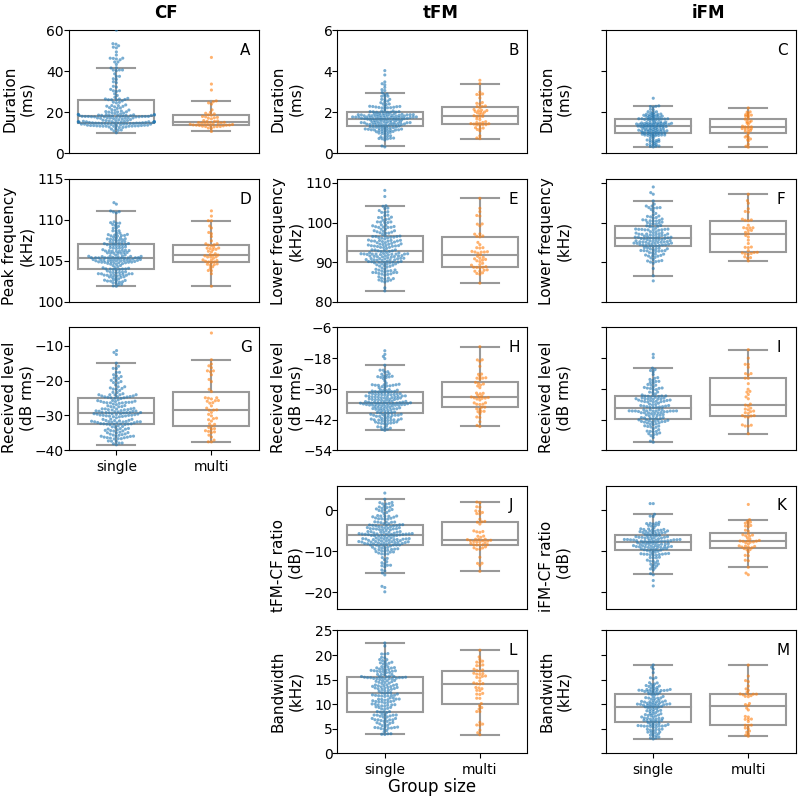
\includegraphics[width=1\linewidth]{original_papers/hbc-paper/combined_analysis/measurements_and_derivedparams_multipanel} \caption{\label{fig:indcallrawdata} Measured acoustic parameters for the constant frequency (CF), initial frequency modulated (iFM) and terminal frequency modulated (tFM) components of individual calls emitted under single-bat and multi-bat conditions. Each column shows the measurements per call component, while each row shows a group of related measurements: A-C) duration D-F) spectral measurements G-I) received level J-K) relative FM-CF ratios L-M) FM component bandwidths. $Ncalls_{single}=$ 177 , $N_{multi-bat}$= 49 . Raw data points are plotted over box plots showing the median, quartiles and whiskers of 1.5 times the inter-quartile range.}\label{fig:indcallrawdata}
\end{figure}

We measured 13 acoustic parameters of the initial and terminal frequency-modulated (iFM, tFM) and of the central constant-frequency (CF) component of 226 individual horseshoe bat echolocation calls (Figure \ref{fig:indcallrawdata}). Most call parameters showed no difference between single-bat and multi-bat observations (Table \ref{tab:alldataindcall}). Only the median duration of the CF-component was \textasciitilde3ms shorter (\emph{p}=0.003) and the median level of the terminal FM-component was \textasciitilde3 dB fainter in multi-bat situations (\emph{p}=0.01) compared to single-bat situations.. The remaining parameters were very similar between the single-bat and multi-bat conditions (p\textgreater0.05, Table \ref{tab:alldataindcall}). For instance, some call parameters that showed change in previous studies had overlapping ranges such as tFM duration (single-bat: 0.32-4.04, multi-bat :0.72-3.57 ), tFM bandwidth (single-bat: 3.85-22.45, multi-bat :3.81-20.98 ) and CF peak frequency (single-bat: 101.9-112.1, multi-bat: 101.9-111.1 ) (See SI \ref{indcallparamranges} for all parameter ranges).

Our `whole dataset' results somewhat matched the results from the `clustered' and `isolated' subsets (SI \ref{subsetsindcall}). Median CF duration differed by \textasciitilde3ms in both isolated and clustered subsets, while iFM and tFM median durations differed by \textasciitilde{} 0.1ms. The spectral parameters (CF peak frequency, tFM bandwidth, i/tFM lower frequency) differed in the magnitude of difference across the `clustered' and `isolated' subsets. If pseudo-replication was not a major concern, we expect the results of the isolated and clustered datasets to match. The observed deviations imply that pseudo-replication may have been a concern however. Before reaching this conclusion, it is important to consider the severe drop in sample size in the isolated data subset as a possible cause for the deviation in trends across parameters. In the isolated subset, \(N_{multi}\) = 5 calls, in contrast to the much higher \(N_{single}\)=53. The severe drop in sample size in the `isolated' data set and the different trends in the spectral parameters make it hard to conclude whether pseudo-replication has played a major role in the individual call analysis.

\begin{verbatim}
## 
## Attaching package: 'flextable'
\end{verbatim}

\begin{verbatim}
## The following objects are masked from 'package:kableExtra':
## 
##     as_image, footnote
\end{verbatim}

\providecommand{\docline}[3]{\noalign{\global\setlength{\arrayrulewidth}{#1}}\arrayrulecolor[HTML]{#2}\cline{#3}}

\setlength{\tabcolsep}{8pt}

\renewcommand*{\arraystretch}{1.5}

\begin{table}

\centering

\begin{longtable}{|p{2.55in}|p{1.85in}|p{1.87in}}

\caption{\label{tab:alldataindcall} *Difference between multi and single bat call parameters. The median difference is reported for all parameters except CF peak frequency, where the difference in range is reported.*}\label{tab:alldataindcall}\\

\hhline{>{\arrayrulecolor[HTML]{000000}\global\arrayrulewidth=2pt}->{\arrayrulecolor[HTML]{000000}\global\arrayrulewidth=2pt}->{\arrayrulecolor[HTML]{000000}\global\arrayrulewidth=2pt}-}

\multicolumn{1}{!{\color[HTML]{000000}\vrule width 0pt}>{\raggedright}p{\dimexpr 2.55in+0\tabcolsep+0\arrayrulewidth}}{\fontsize{11}{13}\selectfont{\textcolor[HTML]{000000}{\global\setmainfont{Arial}Measurement}}} & \multicolumn{1}{!{\color[HTML]{000000}\vrule width 0pt}>{\raggedright}p{\dimexpr 1.85in+0\tabcolsep+0\arrayrulewidth}}{\fontsize{11}{13}\selectfont{\textcolor[HTML]{000000}{\global\setmainfont{Arial}Difference (Multi-Single)}}} & \multicolumn{1}{!{\color[HTML]{000000}\vrule width 0pt}>{\raggedright}p{\dimexpr 1.87in+0\tabcolsep+0\arrayrulewidth}!{\color[HTML]{000000}\vrule width 0pt}}{\fontsize{11}{13}\selectfont{\textcolor[HTML]{000000}{\global\setmainfont{Arial}Permutation test p-value}}} \\

\noalign{\global\setlength{\arrayrulewidth}{2pt}}\arrayrulecolor[HTML]{000000}\cline{1-3}

\endfirsthead

\hhline{>{\arrayrulecolor[HTML]{000000}\global\arrayrulewidth=2pt}->{\arrayrulecolor[HTML]{000000}\global\arrayrulewidth=2pt}->{\arrayrulecolor[HTML]{000000}\global\arrayrulewidth=2pt}-}

\multicolumn{1}{!{\color[HTML]{000000}\vrule width 0pt}>{\raggedright}p{\dimexpr 2.55in+0\tabcolsep+0\arrayrulewidth}}{\fontsize{11}{13}\selectfont{\textcolor[HTML]{000000}{\global\setmainfont{Arial}Measurement}}} & \multicolumn{1}{!{\color[HTML]{000000}\vrule width 0pt}>{\raggedright}p{\dimexpr 1.85in+0\tabcolsep+0\arrayrulewidth}}{\fontsize{11}{13}\selectfont{\textcolor[HTML]{000000}{\global\setmainfont{Arial}Difference (Multi-Single)}}} & \multicolumn{1}{!{\color[HTML]{000000}\vrule width 0pt}>{\raggedright}p{\dimexpr 1.87in+0\tabcolsep+0\arrayrulewidth}!{\color[HTML]{000000}\vrule width 0pt}}{\fontsize{11}{13}\selectfont{\textcolor[HTML]{000000}{\global\setmainfont{Arial}Permutation test p-value}}} \\

\noalign{\global\setlength{\arrayrulewidth}{2pt}}\arrayrulecolor[HTML]{000000}\cline{1-3}\endhead



\multicolumn{1}{!{\color[HTML]{000000}\vrule width 0pt}>{\raggedright}p{\dimexpr 2.55in+0\tabcolsep+0\arrayrulewidth}}{\fontsize{11}{13}\selectfont{\textcolor[HTML]{000000}{\global\setmainfont{Arial}CF duration (median ms)}}} & \multicolumn{1}{!{\color[HTML]{000000}\vrule width 0pt}>{\raggedright}p{\dimexpr 1.85in+0\tabcolsep+0\arrayrulewidth}}{\fontsize{11}{13}\selectfont{\textcolor[HTML]{000000}{\global\setmainfont{Arial}-2.95}}} & \multicolumn{1}{!{\color[HTML]{000000}\vrule width 0pt}>{\raggedright}p{\dimexpr 1.87in+0\tabcolsep+0\arrayrulewidth}!{\color[HTML]{000000}\vrule width 0pt}}{\fontsize{11}{13}\selectfont{\textcolor[HTML]{000000}{\global\setmainfont{Arial}0.003}}} \\





\multicolumn{1}{!{\color[HTML]{000000}\vrule width 0pt}>{\raggedright}p{\dimexpr 2.55in+0\tabcolsep+0\arrayrulewidth}}{\fontsize{11}{13}\selectfont{\textcolor[HTML]{000000}{\global\setmainfont{Arial}tFM duration (median ms)}}} & \multicolumn{1}{!{\color[HTML]{000000}\vrule width 0pt}>{\raggedright}p{\dimexpr 1.85in+0\tabcolsep+0\arrayrulewidth}}{\fontsize{11}{13}\selectfont{\textcolor[HTML]{000000}{\global\setmainfont{Arial}0.14}}} & \multicolumn{1}{!{\color[HTML]{000000}\vrule width 0pt}>{\raggedright}p{\dimexpr 1.87in+0\tabcolsep+0\arrayrulewidth}!{\color[HTML]{000000}\vrule width 0pt}}{\fontsize{11}{13}\selectfont{\textcolor[HTML]{000000}{\global\setmainfont{Arial}0.16}}} \\





\multicolumn{1}{!{\color[HTML]{000000}\vrule width 0pt}>{\raggedright}p{\dimexpr 2.55in+0\tabcolsep+0\arrayrulewidth}}{\fontsize{11}{13}\selectfont{\textcolor[HTML]{000000}{\global\setmainfont{Arial}iFM duration (median ms)}}} & \multicolumn{1}{!{\color[HTML]{000000}\vrule width 0pt}>{\raggedright}p{\dimexpr 1.85in+0\tabcolsep+0\arrayrulewidth}}{\fontsize{11}{13}\selectfont{\textcolor[HTML]{000000}{\global\setmainfont{Arial}-0.04}}} & \multicolumn{1}{!{\color[HTML]{000000}\vrule width 0pt}>{\raggedright}p{\dimexpr 1.87in+0\tabcolsep+0\arrayrulewidth}!{\color[HTML]{000000}\vrule width 0pt}}{\fontsize{11}{13}\selectfont{\textcolor[HTML]{000000}{\global\setmainfont{Arial}0.7}}} \\





\multicolumn{1}{!{\color[HTML]{000000}\vrule width 0pt}>{\raggedright}p{\dimexpr 2.55in+0\tabcolsep+0\arrayrulewidth}}{\fontsize{11}{13}\selectfont{\textcolor[HTML]{000000}{\global\setmainfont{Arial}CF peak frequency (range kHz)}}} & \multicolumn{1}{!{\color[HTML]{000000}\vrule width 0pt}>{\raggedright}p{\dimexpr 1.85in+0\tabcolsep+0\arrayrulewidth}}{\fontsize{11}{13}\selectfont{\textcolor[HTML]{000000}{\global\setmainfont{Arial}-1}}} & \multicolumn{1}{!{\color[HTML]{000000}\vrule width 0pt}>{\raggedright}p{\dimexpr 1.87in+0\tabcolsep+0\arrayrulewidth}!{\color[HTML]{000000}\vrule width 0pt}}{\fontsize{11}{13}\selectfont{\textcolor[HTML]{000000}{\global\setmainfont{Arial}0.18}}} \\





\multicolumn{1}{!{\color[HTML]{000000}\vrule width 0pt}>{\raggedright}p{\dimexpr 2.55in+0\tabcolsep+0\arrayrulewidth}}{\fontsize{11}{13}\selectfont{\textcolor[HTML]{000000}{\global\setmainfont{Arial}tFM lower frequency (median kHz)}}} & \multicolumn{1}{!{\color[HTML]{000000}\vrule width 0pt}>{\raggedright}p{\dimexpr 1.85in+0\tabcolsep+0\arrayrulewidth}}{\fontsize{11}{13}\selectfont{\textcolor[HTML]{000000}{\global\setmainfont{Arial}-1.03}}} & \multicolumn{1}{!{\color[HTML]{000000}\vrule width 0pt}>{\raggedright}p{\dimexpr 1.87in+0\tabcolsep+0\arrayrulewidth}!{\color[HTML]{000000}\vrule width 0pt}}{\fontsize{11}{13}\selectfont{\textcolor[HTML]{000000}{\global\setmainfont{Arial}0.29}}} \\





\multicolumn{1}{!{\color[HTML]{000000}\vrule width 0pt}>{\raggedright}p{\dimexpr 2.55in+0\tabcolsep+0\arrayrulewidth}}{\fontsize{11}{13}\selectfont{\textcolor[HTML]{000000}{\global\setmainfont{Arial}iFM lower frequency (median kHz)}}} & \multicolumn{1}{!{\color[HTML]{000000}\vrule width 0pt}>{\raggedright}p{\dimexpr 1.85in+0\tabcolsep+0\arrayrulewidth}}{\fontsize{11}{13}\selectfont{\textcolor[HTML]{000000}{\global\setmainfont{Arial}1.07}}} & \multicolumn{1}{!{\color[HTML]{000000}\vrule width 0pt}>{\raggedright}p{\dimexpr 1.87in+0\tabcolsep+0\arrayrulewidth}!{\color[HTML]{000000}\vrule width 0pt}}{\fontsize{11}{13}\selectfont{\textcolor[HTML]{000000}{\global\setmainfont{Arial}0.24}}} \\





\multicolumn{1}{!{\color[HTML]{000000}\vrule width 0pt}>{\raggedright}p{\dimexpr 2.55in+0\tabcolsep+0\arrayrulewidth}}{\fontsize{11}{13}\selectfont{\textcolor[HTML]{000000}{\global\setmainfont{Arial}CF level (median dB RMS)}}} & \multicolumn{1}{!{\color[HTML]{000000}\vrule width 0pt}>{\raggedright}p{\dimexpr 1.85in+0\tabcolsep+0\arrayrulewidth}}{\fontsize{11}{13}\selectfont{\textcolor[HTML]{000000}{\global\setmainfont{Arial}-1.48}}} & \multicolumn{1}{!{\color[HTML]{000000}\vrule width 0pt}>{\raggedright}p{\dimexpr 1.87in+0\tabcolsep+0\arrayrulewidth}!{\color[HTML]{000000}\vrule width 0pt}}{\fontsize{11}{13}\selectfont{\textcolor[HTML]{000000}{\global\setmainfont{Arial}0.2}}} \\





\multicolumn{1}{!{\color[HTML]{000000}\vrule width 0pt}>{\raggedright}p{\dimexpr 2.55in+0\tabcolsep+0\arrayrulewidth}}{\fontsize{11}{13}\selectfont{\textcolor[HTML]{000000}{\global\setmainfont{Arial}tFM level (median dB RMS)}}} & \multicolumn{1}{!{\color[HTML]{000000}\vrule width 0pt}>{\raggedright}p{\dimexpr 1.85in+0\tabcolsep+0\arrayrulewidth}}{\fontsize{11}{13}\selectfont{\textcolor[HTML]{000000}{\global\setmainfont{Arial}-3.15}}} & \multicolumn{1}{!{\color[HTML]{000000}\vrule width 0pt}>{\raggedright}p{\dimexpr 1.87in+0\tabcolsep+0\arrayrulewidth}!{\color[HTML]{000000}\vrule width 0pt}}{\fontsize{11}{13}\selectfont{\textcolor[HTML]{000000}{\global\setmainfont{Arial}0.01}}} \\





\multicolumn{1}{!{\color[HTML]{000000}\vrule width 0pt}>{\raggedright}p{\dimexpr 2.55in+0\tabcolsep+0\arrayrulewidth}}{\fontsize{11}{13}\selectfont{\textcolor[HTML]{000000}{\global\setmainfont{Arial}iFM level (median dB RMS)}}} & \multicolumn{1}{!{\color[HTML]{000000}\vrule width 0pt}>{\raggedright}p{\dimexpr 1.85in+0\tabcolsep+0\arrayrulewidth}}{\fontsize{11}{13}\selectfont{\textcolor[HTML]{000000}{\global\setmainfont{Arial}-1.66}}} & \multicolumn{1}{!{\color[HTML]{000000}\vrule width 0pt}>{\raggedright}p{\dimexpr 1.87in+0\tabcolsep+0\arrayrulewidth}!{\color[HTML]{000000}\vrule width 0pt}}{\fontsize{11}{13}\selectfont{\textcolor[HTML]{000000}{\global\setmainfont{Arial}0.32}}} \\





\multicolumn{1}{!{\color[HTML]{000000}\vrule width 0pt}>{\raggedright}p{\dimexpr 2.55in+0\tabcolsep+0\arrayrulewidth}}{\fontsize{11}{13}\selectfont{\textcolor[HTML]{000000}{\global\setmainfont{Arial}tFM-CF ratio (median dB)}}} & \multicolumn{1}{!{\color[HTML]{000000}\vrule width 0pt}>{\raggedright}p{\dimexpr 1.85in+0\tabcolsep+0\arrayrulewidth}}{\fontsize{11}{13}\selectfont{\textcolor[HTML]{000000}{\global\setmainfont{Arial}-1.08}}} & \multicolumn{1}{!{\color[HTML]{000000}\vrule width 0pt}>{\raggedright}p{\dimexpr 1.87in+0\tabcolsep+0\arrayrulewidth}!{\color[HTML]{000000}\vrule width 0pt}}{\fontsize{11}{13}\selectfont{\textcolor[HTML]{000000}{\global\setmainfont{Arial}0.16}}} \\





\multicolumn{1}{!{\color[HTML]{000000}\vrule width 0pt}>{\raggedright}p{\dimexpr 2.55in+0\tabcolsep+0\arrayrulewidth}}{\fontsize{11}{13}\selectfont{\textcolor[HTML]{000000}{\global\setmainfont{Arial}iFM-CF ratio (median dB)}}} & \multicolumn{1}{!{\color[HTML]{000000}\vrule width 0pt}>{\raggedright}p{\dimexpr 1.85in+0\tabcolsep+0\arrayrulewidth}}{\fontsize{11}{13}\selectfont{\textcolor[HTML]{000000}{\global\setmainfont{Arial}0.25}}} & \multicolumn{1}{!{\color[HTML]{000000}\vrule width 0pt}>{\raggedright}p{\dimexpr 1.87in+0\tabcolsep+0\arrayrulewidth}!{\color[HTML]{000000}\vrule width 0pt}}{\fontsize{11}{13}\selectfont{\textcolor[HTML]{000000}{\global\setmainfont{Arial}0.75}}} \\





\multicolumn{1}{!{\color[HTML]{000000}\vrule width 0pt}>{\raggedright}p{\dimexpr 2.55in+0\tabcolsep+0\arrayrulewidth}}{\fontsize{11}{13}\selectfont{\textcolor[HTML]{000000}{\global\setmainfont{Arial}tFM bandwidth (median kHz)}}} & \multicolumn{1}{!{\color[HTML]{000000}\vrule width 0pt}>{\raggedright}p{\dimexpr 1.85in+0\tabcolsep+0\arrayrulewidth}}{\fontsize{11}{13}\selectfont{\textcolor[HTML]{000000}{\global\setmainfont{Arial}1.83}}} & \multicolumn{1}{!{\color[HTML]{000000}\vrule width 0pt}>{\raggedright}p{\dimexpr 1.87in+0\tabcolsep+0\arrayrulewidth}!{\color[HTML]{000000}\vrule width 0pt}}{\fontsize{11}{13}\selectfont{\textcolor[HTML]{000000}{\global\setmainfont{Arial}0.12}}} \\





\multicolumn{1}{!{\color[HTML]{000000}\vrule width 0pt}>{\raggedright}p{\dimexpr 2.55in+0\tabcolsep+0\arrayrulewidth}}{\fontsize{11}{13}\selectfont{\textcolor[HTML]{000000}{\global\setmainfont{Arial}iFM bandwidth (median kHz)}}} & \multicolumn{1}{!{\color[HTML]{000000}\vrule width 0pt}>{\raggedright}p{\dimexpr 1.85in+0\tabcolsep+0\arrayrulewidth}}{\fontsize{11}{13}\selectfont{\textcolor[HTML]{000000}{\global\setmainfont{Arial}0.27}}} & \multicolumn{1}{!{\color[HTML]{000000}\vrule width 0pt}>{\raggedright}p{\dimexpr 1.87in+0\tabcolsep+0\arrayrulewidth}!{\color[HTML]{000000}\vrule width 0pt}}{\fontsize{11}{13}\selectfont{\textcolor[HTML]{000000}{\global\setmainfont{Arial}0.82}}} \\

\noalign{\global\setlength{\arrayrulewidth}{2pt}}\arrayrulecolor[HTML]{000000}\cline{1-3}

\end{longtable}

\end{table}

\hypertarget{windowed-call-analysis-1}{%
\subsection{Windowed call analysis}\label{windowed-call-analysis-1}}

We split flight-activity audio into 50ms windows duration and analysed two parameters for each window: received level and FM lower frequency (\(Nfiles_{single}\)=233,\(Nfiles_{multi}=\) 87). For each flight-activity audio we also measured the dominant-frequency range (maximum -- minimum dominant frequency of all windows in that audio). Dominant frequency ranges indicate the amount of shifting or convergence in the CF frequencies within a flight activity (Figure \ref{fig:domfreqgraph}). An increase in frequency range indicates a reduced frequency overlap, while a decrease in frequency range indicates a convergence of frequencies. The median dominant frequency range (Figure \ref{fig:domfreqgraph}) was 2.2 kHz larger (\emph{p}\textless10\(^{-4}\)) in multi-bat conditions (range:0.03-7.65 kHz) compared to the single-bat condition (range:0.02-2.86 kHz). The observed median difference in dominant frequency range matches the magnitude in simulations when bats do not show any special responses to each other (SI \ref{simdomfreqranges}). The observed difference in median dominant frequency range matches The estimated median differences for received level (95\(\%\)ile range:-0.88-1.61 dB) and FM lower frequency (95\(\%\)ile range: -1.46-0.98 kHz) showed no systematic trend, indicating no relative increase or decrease. Subset analysis also revealed the same trends in both isolated and clustered data for multi-bat and single-bat comparisons (SI \ref{subsetswincall}). Both isolated and clustered subsets showed a dominant frequency range difference of \textasciitilde{} 2 kHz. The median difference ranges of both received level and FM lower frequency were similarly located on either of zero. Isolated and clustered subsets showed the same trends with an increased dominant frequency range of \textasciitilde2 kHz and with estimated received level and lower frequency median differences on either side of zero (SI \ref{subsetswincall}).

\begin{figure}
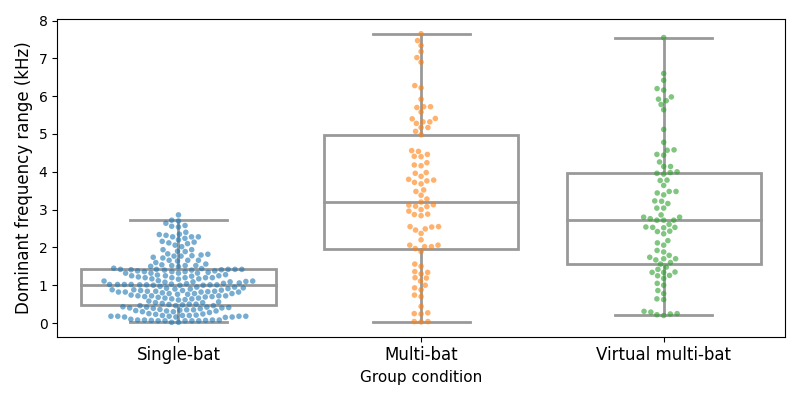
\includegraphics[width=1\linewidth]{original_papers/hbc-paper/combined_analysis/domfreqranges} \caption{\label{domfreqgraph} Measured dominant frequency range (max-min) across flight activities in single-bats, multi-bat and virtual multi-bat conditions. Variation in dominant frequency in single-bat condition arises from the combination of active Doppler-shift compensation by the bat and Doppler-shift due to bat flight past the microphone. The dominant frequency range in multi-bat and virtual multi-bat is larger because of there are more than one bat. The median multi-bat dominant frequency range is greater than single-bat range by 2.2 kHz (*p*<10$^{-4}$). Virtual multi-bat and multi-bat median range difference was much lower and negligible at 0.48 kHz (*p*=0.16)}\label{fig:domfreqgraph}
\end{figure}

Median difference in dominant frequency range in the multi-bat was relatively low at 0.48 kHz more (\emph{p}=0.16) than the virtual-multi-bat condition (range:0.2-7.55 kHz). Median differences of received level (95\(\%\)ile range:-0.72-2.1 dB) and FM lower frequency (95\(\%\)ile range:-1.95-0.98 kHz) indicate no systematic trend towards a relative increase or decrease in multi-bat windows in comparison to virtual-multi bat. Subset analysis also revealed similar trends (SI \ref{subsetswincall}). Isolated and clustered subsets showed similarly low dominant frequency range differences of between 0-0.6 kHz. For both subsets, received level and lower frequency the estimated median difference range was on either side of zero.

The results of both window-analysis reveals a consistency between the isolated and clustered subsets, hints at the possibility that pseudo-replication may not be an issue. Even though the parameter trends match, here too, the isolated subsets suffered from a drop in sample size, with \(N_{multi-bat}=8\), in comparison to \(N_{multi-bat}=79\) in the clustered subset.

\hypertarget{discussion-1}{%
\section{Discussion}\label{discussion-1}}

We quantified the difference in horseshoe bat echolocation calls when alone and with conspecifics in the field. Our results do not support a biologically meaningful difference in echolocation calls with reference to group size for all of the call parameters measured using two different approaches. This may seem somewhat unexpected, especially considering the fact that bats in our field site were flying in an enclosed reverberant volume - which would only amplify the problem of masking in multi-bat echolocation. We interpret our results below in more detail.

To address the problem of analyzing calls that overlap in time and frequency, we introduced two automated analyses that can be performed on audio recordings of multiple CF-FM bats. First, we performed automated individual call analyses using the open-source \texttt{itsfm} package allows call component segmentation based on rate of frequency change in a sound. This frequency-modulation-based segmentation performs better than filtering around the peak frequency and results in more accurate CF-FM call component segmentation, and thus better measurements. \citep{itsfmcitation}. Second, to analyse audio with overlapping calls, we measured the overall acoustic parameters of short audio windows without assigning the measurements to individual calls. While coarser in time than the individual call analysis, this window-based approach complements the individual call analyses by returning related measurements such as FM terminal frequency and dominant frequency range.

\hypertarget{cf-component}{%
\subsection{CF component}\label{cf-component}}

To avoid spectral overlap in groups, the spectral jamming avoidance response (JAR) hypothesis predicts that individual bats in groups will shift their call frequencies away from those of other individuals \citep{ulanovsky2004dynamics}. JAR has mixed support from studies. Several studies in hipposiderid \& rhinolophid bats found no changes in CF frequencies \citep{jones1993echolocation, jones1994individual, fawcett2015clutter, pye1972bimodal}. In contrast, \citet{habersetzer1981adaptive} observed CF frequency shifting in groups of the quasi-CF rhinopomatid bat , \emph{Rhinopoma hardwickei}, while \citet{cvikel2015b} found no support in the same species. However, the echolocation of R. hardwickei is not entirely comparable with those of the more specialised CF-bats of the families Hipposideridae and Rhinlophidae \citep{simmons1984echolocation}. Hipposiderids and rhinolophids are more constrained in their echolocation as they show a marked individual-specific acoustic fovea that does not vary over short periods of time \citep{neuweiler2000biology, schnitzler1976peripheral}. CF-FM bats are thus constrained to emit calls so that the Doppler-shifted echoes arrive within their own acoustic fovea's range.

Our data does not support CF frequency shifting in groups. If bats were to show `jamming avoidance' type responses, one would expect an overall increase in the CF frequency range in groups, and thus an increased range difference between single and multi bat audio. If they were to show `convergence' ), we expect a reduction in range. The observed CF and dominant frequency range differences of around 2 kHz between single and multi bats falls within the expected magnitude seen when bats do not show any special responses to each other (SI \ref{simdomfreqranges}). More convincingly however, the low difference in dominant frequency range between multi and virtual multi audio shows that even when bats are indeed flying together they are not actively altering their CF frequencies to reduce or increase overlap. Our simulations (SI \ref{simdomfreqranges}) and single bat experimental audio data show that a receiver (eg. a microphone or another bat) placed in the proximity of a flying CF-FM bat may hear a series of CF frequencies that vary by upto \(\pm\) 3 kHz from the emitted frequency. This relatively large variation in the received frequency thus decreases the extent of spectral overlaps during multi-bat echolocation. The combination of individual specific acoustic foveas and Doppler-shift driven variation in received CF frequency make it unlikely that the CF component would be masked effectively even in groups. For the duration of CF component , we found a median decrease by around 3 ms in multi-bat calls, matching the decrease by \textasciitilde1.2 ms found by Fawcett et al.~(2015). Note that our procedure of selecting non-overlapping calls in the individual call analysis might bias our selection to shorter calls in multi-bat recordings, because shorter calls might be less prone to temporal overlap. The bias is not very evident in our data however, as the range of CF durations (the longest part of a CF-FM call) overlap in both single-bat and multi-bat conditions.

\hypertarget{fm-component}{%
\subsection{FM component}\label{fm-component}}

The FM component is likely used for ranging and undergoes large variation as bats approach objects \citep{Fenton2014}. Frequency-changes in group flying FM-bats could indicate a JAR, but could also be a response to the physical presence of other bats in the vicinity \citep{cvikel2015b, fawcett2015clutter}. CF-FM bats also show alterations in their tFM as they approach and land \citep{tian1997echolocation, schoeppler2018precise, Fenton2014}, and may be expected to respond to conspecifics like FM-bats in groups. Fawcett et al.~(2015) found that the tFM minimum frequency (-10 dB call peak frequency) increase by 5 kHz on average in pairs. In contrast, we only found a drop by \textasciitilde1 kHz of the tFM lower frequency (-10 dB tFM peak frequency) and an increase by maximally 1.8 kHz of tFM bandwidth. Our window analysis revealed no systematic differences in terminal frequency estimates between single-bat and multi-bat situations. Both FM and CF-FM bats also change call duration in the presence of conspecifics and noise \citep[\citet{gomes2020individual}]{cvikel2015b, amichai2015calling, fawcett2015echolocation, lu2020echolocating}. While we found only found an increase in tFM duration by 0.1 ms, previous studies found 0.6-1.8 ms. \citet{fawcett2015echolocation} found an average increase in tFM duration by 1.8 ms in pairs, while we find a slight median increase by about 0.1 ms in multi-bat calls. In another study with artifical playbacks, \citet{lu2020echolocating} found an increase of 0.6ms in comparison to calls in silence. An increased tFM duration may provide an increase in in echo detection \citep{amichai2015calling, luo2015linking}. The current increase in duration corresponds to a negligible fraction (\textasciitilde5\%), and is unlikely to have any major sensory implications. Compared to previous studies, our effects are small, and unlikely to have biological relevance.

\hypertarget{call-level}{%
\subsection{Call level}\label{call-level}}

CF-FM Bats increase call source levels in the presence of experimental playbacks \citep{hage2013ambient, hage2014ambient, lu2020echolocating}. In our study, we could not measure the bats source level because bats were free-flying and we did not track their 3D-position. Instead, we analysed the received level at the microphone. In addition to the bat's source level, received levels also depend on the bats' distance to and calling direction relative to the microphone. The received level of the tFM of individual calls was 3dB lower median in the multi-bat condition than in the single-bat condition, while the difference was only \textasciitilde1.5 dB in the iFM and CF components. The windowed call analysis revealed no systematic alteration in received level in multi-bat vs single-bat and in multi-bat vs.~virtual-multi-bat conditions. The relative received levels between the CF and FM components changed by around 1 dB between the multi-bat and single-bat conditions, indicating no shift in call energy between the components. Why was there no major difference in received levels between single-bat and multi-bat conditions even in the window analysis, where overlapping calls are expected to lead to a higher received level? The similarity in received levels of multi-bat and single-bat windows can be explained by the inequal contribution the nearest bat's call makes to the received level due to spherical spreading, and the directionality of calls. The fact that multi-bat and virtual-multi bat audio have similar received levels thus indirectly suggests there is no change in source level even in the presence of another bat. However, the tFM received level showed a drop of around 3dB that we are not sure how to interpret. This apparent drop in received level could be the result of bats flying further away or emitting more directional calls.

\hypertarget{outlook}{%
\subsection{Outlook}\label{outlook}}

There are a set of parameters that we were not able to measure and thus excluded in our analyses. We did not measure call-sequence related parameters such as inter-call-intervals or duty-cycle. Bats in acoustically difficult situations are known to alter their call rate \citep{amichai2015calling, jarvis2013groups} and thus their duty cycle. Measuring inter-call-intervals is possible in single bat contexts, but extremely challenging in multi-bat recordings with overlapping calls and reverberation. Calls are difficult to assign to their source individuals, which complicates call interval measurement.

What are the possible explanations for the absence of a strong echolocation response in groups? Our data suggests that echolocation in groups with a few bats (2-4) bats may not be very challenging for multiple reasons. CF-FM bats rely on the tFM component to detect the distance of objects around them \citep{tian1997echolocation}. The tFM components are short (\(\leq\) 3.4ms, 95 percentile value), and likely emitted every 40-50 ms which is equivalent to a tFM duty cycle between 6.8-8.5\%. For a pair of bats at these duty cycles, the probability of one tFM echo being overlapped by another bat's tFM call component is relatively low at most between 1.6 - 2.1\% (SI \ref{simtfmoverlap} for calculations). Even if a single tFM echo is overlapped by another call, a bat may still be able to detect it if the signal-to-noise ratio is sufficient. FM bats in small groups are unlikely to face major detriments to their echolocation \citep{beleyur2019modeling}, which should also apply to using the FM for ranging, explaining why the horseshoe bats did not show call changes from solitary echolocation. Secondly, \citet{fawcett2015echolocation} observed an increased tFM duration and bandwidth in R. capensis flying in pairs in a novel flight room setting. The combination of flight room characteristics \citep{surlykke2009echolocating} and species differences, may perhaps have led to the difference in results between their study and ours. Bats show long-term spatial memory \citep{barchi2013spatial, mohres1949versuche} and familiarity with the cave's structure may have allowed them to easily recognise their location over time. Bats also use echoes across multiple calls and are thus resistant to occasional disruptions in echo arrival \citep{Salles202011719}. The combination of spatial memory and multi-echo integration may have allowed our bats to continue echolocating with conspecifics without altering their calls drastically.

It is well established that bats adapt and alter their echolocation strategy in the face of sensory challenge. Our results add a subtle twist to the literature by suggesting that bats may not always employ a special echolocation strategy even when faced with the sensory challenge of a group. We highlight the importance of observational studies in field settings to understand the frequency with which various sensory strategies are actually employed in ecological contexts.

\hypertarget{data-and-code-availability}{%
\section{Data and code availability}\label{data-and-code-availability}}

All data and code used process data and generate the results and figures in the paper are available at the following Github repository: \url{https://github.com/thejasvibr/mhbc-online/}

\hypertarget{acknowledgements-2}{%
\section{Acknowledgements}\label{acknowledgements-2}}

The authors would like to specially thank the electronics team (Markus Abels, Hannes Sagunsky, Reinhard Biller) at the MPIO workshop for help preparing the electronic circuits to run the ON/OFF signal splitting. We would also like to thank Antoniya Hubancheva for logistical support, Stefan Greif for help collecting the data, the 2018 Tabachka field crew, Klaus Hochradel for the point-cloud scan of the cave and Diana Schoeppler and Hans-Ulrich Schnitzler for their helpful discussions. We also thank Manjari Jain for her support and and encouragement of the project. TB was funded by a DAAD doctoral fellowship and the IMPRS for Organismal Biology, HRG was funded by the Emmy Noether program of the DFG (German Research Foundation, grant no. 241711556)

\hypertarget{author-contributions}{%
\section{Author Contributions}\label{author-contributions}}

Study design and conception: NMR, TB; Data collection: AK, NMR, TB; Audio and video annotation: AK, NMR; Audio-video synchronisation: TB; Analysis: HRG, NMR, TB; Interpretation of results: HRG, NMR, TB; Manuscript preparation: HRG, NMR, TB.

\newpage

\hypertarget{supplementary-information-1}{%
\section{Supplementary Information}\label{supplementary-information-1}}

\hypertarget{avmatching}{%
\subsection{Audio-video synchronisation: hardware and software implementations}\label{avmatching}}

The audio and video data were synchronised using the protocol of \citep{laurijssen2018low}. A Raspberry Pi 3 was used to drive an ON/OFF signal from a GPIO port. This ON/OFF signal was then split between an LED and a circuit linked to capacitor. The capacitor converted the DC ON/OFF signal into positive and negative spikes - thus allowing the signal to be correctly digitised. Not all soundcards are capable of digitising DC voltages, and thus the capacitor helps in making the protocol independent of soundcard type. The entire circuit can be assembled from easily available parts (Figures \ref{fig:breadboard}, \ref{fig:circuitschematic})

\begin{figure}
\includegraphics[width=1\linewidth]{original_papers/hbc-paper/figures/breadboard_circuit_trim_labelled} \caption{\label{fig:breadboard} The experimental realisation of the audio-video synchronisation signal splitting. The components can easily be assembled onto a hobby breadboard, and are easily portable. Here the breadboard is pasted on the inside of a lunch box lid, allowing easy and safe transport of the breadboard and the Raspberry Pi in the box itself.}\label{fig:breadboard}
\end{figure}

\begin{figure}
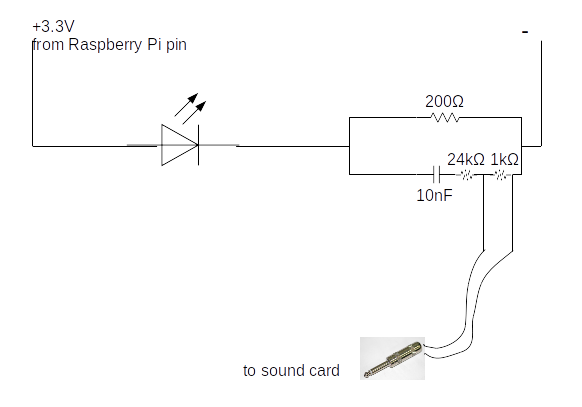
\includegraphics[width=1\linewidth]{original_papers/hbc-paper/figures/rpi_circuit} \caption{\label{fig:circuitschematic} The circuit plan of the synchronisation signal splitter shown in Figure \\ref{fig:breadboard}}\label{fig:circuitschematic}
\end{figure}

The code to drive the GPIO port runs on Python 2 (and should also run on Python 3). For best results the python file
can be set to automatically run on boot-up. This makes the synchronisation protocol field-friendly, and reduces the need
of the experimenter manually running the code.

\begin{verbatim}
#!/usr/bin/python
'''
script that switches a RED LED on and off
This script and the circuit used to
run the system is based on the post at thePiHut
'Turning on an LED with your Raspberry Pi's GPIO Pins' 
URL: https://thepihut.com/blogs/raspberry-pi-tutorials/
27968772-turning-on-an-led-with-your-raspberry-pis-gpio-pins
Accessed June 11 2015
'''
import RPi.GPIO as GPIO
import sys
import time
GPIO.setmode(GPIO.BCM)
GPIO.setwarnings(False)
GPIO.setup(18,GPIO.OUT)
import numpy as np

time_ranges = np.arange(0.08,0.5,0.0001)

while True:
    try:
        #print ('LED ON')
        GPIO.output(18,True)
        on_time = np.random.choice(time_ranges,1)
        time.sleep(on_time)
        #print('LED OFF')
        off_time = np.random.choice(time_ranges,1)
        GPIO.output(18,False)
        time.sleep(off_time)
    except KeyboardInterrupt:
        GPIO.output(18,GPIO.LOW)
        sys.exit()
\end{verbatim}

One optional change that can be made to the code above is to set the seed manually with \texttt{np.random.seed} after the numpy import.
Setting a fixed seed can have the advantage that problems in audio-video file synchronisation post data collection can be better
fixed. A fixed seed however means that the output signal is the same across all sessions used - which might make distinguishing
audio and video recordings from different sessions difficult, though not exclude it.

Another important aspect to pay attention to is the \texttt{time\_ranges} variable. In this experiment it was assumed that the camera frame rate
was going to be 25 Hz, and thus the lowest ON/OFF time was set to 0.08s, which corresponds to a signal with 12.5Hz periodicity of the Nyquist frequency. However, as \citet{laurijssen2018low} suggest, it would have been better to set the lowest duration to a longer period, which was a few times lower than the Nyquist frequency of 12.5 Hz, eg. 0.2s (5 Hz). In our experiments, the cameras turned out to have a frame rate of 22Hz, which meant that the LED signal was aliased. However, despite the
aliasing, we were still able to synchronise audio and video - showing the robustness of the methodology.

\hypertarget{video-annotation-of-bat-flight-activity-in-the-cave}{%
\subsection{Video annotation of bat flight activity in the cave}\label{video-annotation-of-bat-flight-activity-in-the-cave}}

Manual annotation of the video data was carried out to determine the group sizes of free-flying horseshoe bats in their natural habitat. We annotated bat flight activity by simultaneously viewing the video feeds from both infrared cameras using SHOTCUT, a free open-source video editing software (REFERENCE and VERSION NUMBER). The following information was documented from the video: the start and end times of bat flight activity from the burnt in timestamps from either camera 1 or 2 in ``yyyy-mm-dd hh:mm:ss'' format, frame number, number of bats flying and flight behavior. A bat flight activity is defined as the interval during which the number of bats flying inside the cave is constant. Successive bat flight activities were operationally defined as being separated from one another by least 6 frames .

We defined the start of bat activity from the frame a bat is observed to fly in either camera view. Similarly, the end of bat flight activity was when a bat is not observed in either of the camera views. In multi-bat contexts that can have dynamic transitions in the number of bats, we annotated the start and end of the multi-bat activity with parts of the video that had the maximum number of bats. Additionally, bat activity before and after the video segment with the maximum number of bats were also annotated as single or multi-bat activity ensuring an interval of 6 frames separating each activity.\\
Video from both the cameras covered most parts of the cave except the roosting sites (Main paper Figure \ref{cavesetupschematic}). Bats were found to fly into the roosting sites, disappearing and then appearing in the camera view for short (=\textless10 frames) or extended periods (\textgreater10 frames) of time. If a bat appeared again after a short period, the current annotation was continued till the end of the activity. If a bat appeared after an extended period, a new annotation was begun.

We prioritized obtaining a clean data set and refrained from annotating extremely difficult bat flight annotations because of how dynamic the group size shifts could be.

\hypertarget{individual-call-analysis-2}{%
\subsection{Individual call analysis}\label{individual-call-analysis-2}}

\hypertarget{indcallprotocol}{%
\subsubsection{Individual call selection}\label{indcallprotocol}}

Individual calls were selected from the audio files based on a set of pre-defined search protocol:

\begin{itemize}
\item
  All measurements and signal processing will be done using Audacity.
\item
  dB rms measurements made with the `Contrast' function in Audacity. Highpassing done with the inbuilt highpass filter. The SNR is calculated by difference between the foreground (bat call region) and background (silent region)

  \begin{enumerate}
  \def\labelenumi{\arabic{enumi}.}
  \tightlist
  \item
    Load annotation audio file, and delete all non-target channels.
  \item
    View audio in spectrogram mode. Set dynamic range of spectrogram to 60dB.
  \item
    Highpass filter audio file with 12 dB roll off/octave at 80 kHz cutoff frequency
  \item
    For given audio file, choose a start point using a random number generator between 0-1.
  \item
    Go to that fraction of time corresponding to the length of the annotation audio file
  \item
    Choose another random number between 0-1. If it's \textless=0.5 search towards left, else search towards right.
  \item
    Look for a horseshoebat call with no overlaps, no interference patterns in the CF or FM, that can be isolated well.
  \item
    While selecting horseshoe bat calls, zoom in max till 60 milliseconds of audio occupy the whole screen. Do not zoom in more or less while selecting.
  \item
    Check the SNR of the selected horseshoe bat call by using a `silent period' of the audio file as background. If there is not suitably long `silent period' to serve as background in this audio file, choose another random audio file and measure the background dB rms.

    \begin{enumerate}
    \def\labelenumii{\alph{enumii}.}
    \tightlist
    \item
      If SNR \textgreater= 20 dB, this is a suitable call to measure. Note down the start and end time of this call in the audio file.
    \item
      If SNR \textless{} 20dB

      \begin{enumerate}
      \def\labelenumiii{\roman{enumiii}.}
      \tightlist
      \item
        Go back to search start point calculated in 4), and begin searching in opposite direction.
      \item
        Look for first suitable call to measure using criteria in 7) onwards.
      \end{enumerate}
    \item
      If a suitable call is still NOT found:

      \begin{enumerate}
      \def\labelenumiii{\roman{enumiii}.}
      \tightlist
      \item
        No measurement takes place in this audio annotation. Proceed to next audio annotation file.
      \end{enumerate}
    \end{enumerate}
  \end{enumerate}
\end{itemize}

Audacity version 2.3.3 was used during the manual call selection.

\hypertarget{windowed-call-analysis-2}{%
\subsection{Windowed call analysis}\label{windowed-call-analysis-2}}

\hypertarget{windowdetails}{%
\subsubsection{Making windows}\label{windowdetails}}

Each flight activity audio was split into consecutive 50ms windows. All tail-end audio that was \textless50 ms was discarded.

\hypertarget{silentwindow}{%
\subsubsection{Choosing the `silent window threshold'}\label{silentwindow}}

A series of manually annotated audio clips were used to set the reference silent window threshold. The manually annotated audio clips were the same as those used to calculate the reference `silence' segments in the individual call analysis (\(N_{files}=406\), min-max duration=0.002-0.03s). The threshold for a window to be chosen as silent was set at 20dB above the maximum measured dB rms of all silent windows. This resulted in any window that was less than -23 dB rms as being considered `silent'. This is a conservative approach that prevents windows with poor signal-to-noise ratio from being analysed.

The code to execute this analysis is available in the \texttt{what\ qualifies\ as\ a\ silent\ audio\ segment.ipynb} notebook and its HTML printout.

\hypertarget{domfreqdetails}{%
\subsubsection{Dominant frequency measurement}\label{domfreqdetails}}

Unlike typical measures used to quantify echolocation calls like peak frequency or-10 dB frequency, the dominant frequencies provide a glimpse of what may be happening in the presence of multiple calls.

The dominant frequency was determined with the following steps:

\begin{enumerate}
\def\labelenumi{\arabic{enumi}.}
\tightlist
\item
  Create a smoothed power spectrum. A smoothed power spectrum is generated by passing the raw spectrum (FFT size = 12500 samples) with a running-mean filter of the pre-defined spectral smoothing width. The spectral smoothing width defines the `width' or the number of frequency bins of the running-mean filter. We used a smoothing width of 100 Hz, which corresponds to 5 frequency bins. The smoothing is necessary as the raw power spectrum can be very `jagged' otherwise, and impede peak detection which corresponds to the CF components of calls in the input audio.
\item
  Extract the peaks in the smoothed power spectrum. Only peaks that are a minimum `distance' from each other, and that are within a threshold of the highest peak are chosen. We chose an inter-peak distance of 250 Hz, and all valid dominant frequency peaks needed to lie within 14 dB of the peak with the highest power.
\item
  Map the valid peaks to the frequencies they correspond to. These are the dominant frequencies in this
\end{enumerate}

The code to execute this function is available in the \texttt{inbuilt\_measurement\_functions.py} module.

\hypertarget{lowestfreqdetails}{%
\subsubsection{FM terminal frequency measurement}\label{lowestfreqdetails}}

The FM terminal frequency (Figure \ref{fig:fmterminal}) is determined in the following steps:

\begin{enumerate}
\def\labelenumi{\arabic{enumi}.}
\tightlist
\item
  Make spectrogram of the audio window (512 samples FFT, 256 samples overlap).
\item
  Identify all spectrogram `pixels' in the FM frequency band that are above the baseline level. The FM bandwidth was defined as ranging from 70 kHz to 98 kHz. The baseline power level across pixels was calculated by calculating the 95\%ile value of power in the frequency band below 70 kHz, i.e., the part of the spectrogram without any bat calls. All pixels whose power was 46 dB above the baseline power level and whose frequency was within 70 - 98 kHz were considered valid FM pixels
\item
  Identify contiguous clusters of FM pixels. These clusters represent single iFM or tFM components of calls.
\item
  From the identified continuous clusters, extract the lowest frequency pixel in a cluster
\end{enumerate}

Given the current parameter values used for our analysis, the terminal frequency measurements have a spectral resolution of 488 Hz.

The code to execute this function is available in the \texttt{inbuilt\_measurement\_functions.py} module.

\begin{figure}
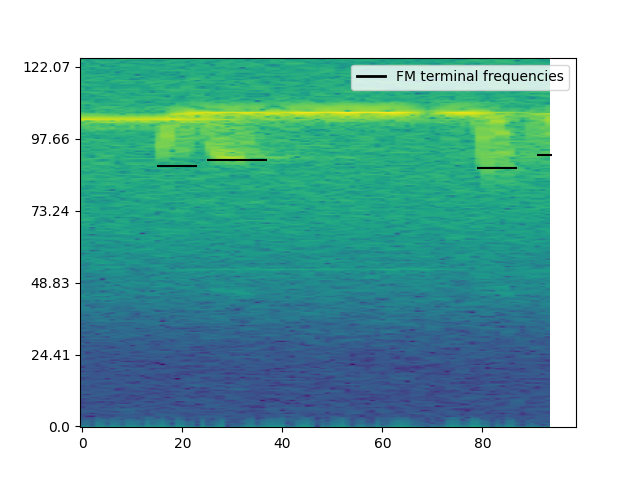
\includegraphics[width=1\linewidth]{original_papers/hbc-paper/figures/fm_terminal_0_matching_annotaudio_Aditya_2018-08-16_2324_231_hp.} \caption{\label{fig:fmterminal}Example showing extracted FM terminal frequencies from the spectrogram of a 50ms window. The method allows extraction of terminal frequencies in the presence of multiple overlapping calls, though it doesn't allow discrimination of iFM and tFM components }\label{fig:fmterminal}
\end{figure}

\hypertarget{virtualdetails}{%
\subsubsection{Making virtual multi bat audio files}\label{virtualdetails}}

\begin{figure}
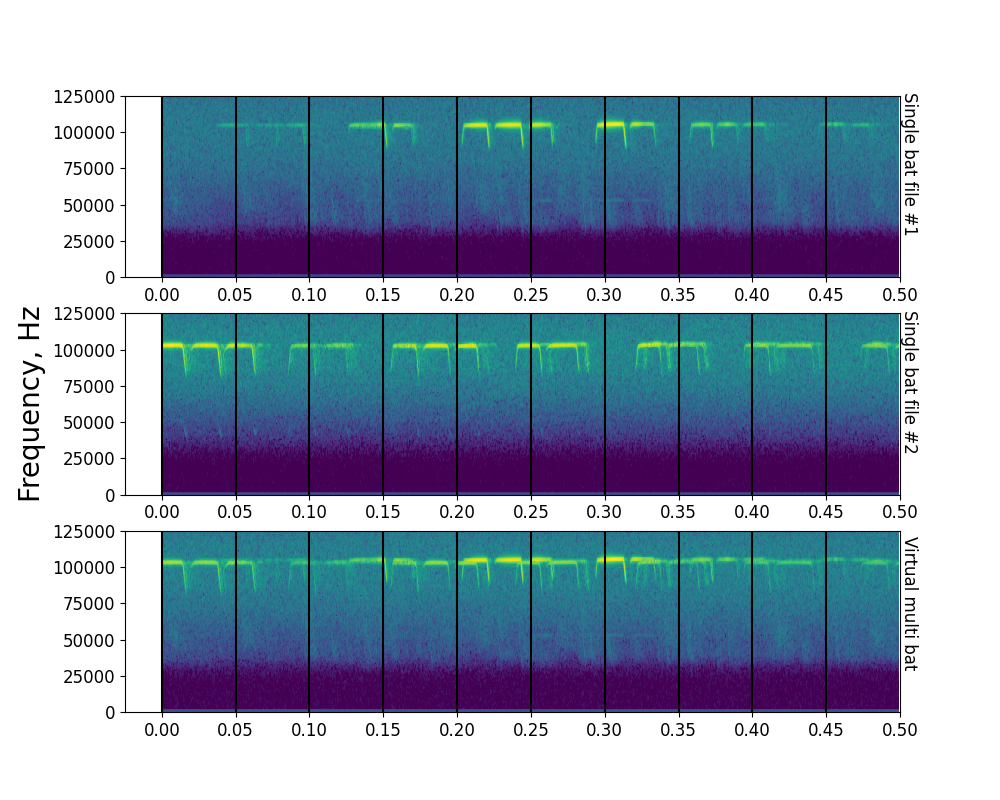
\includegraphics[width=1\linewidth]{original_papers/hbc-paper/figures/figX_virtualmultibat} \caption{\label{fig:virtualmultibat} Example showing the steps involved in creating a virtual multi bat file. Shown here are spectrograms of the first 500ms of two single bat audio files (A), (B), along with the resulting virtual multi bat audio file. Vertical lines delineate 50ms windows that are used for acoustic measurements}\label{fig:virtualmultibat}
\end{figure}

Virtual multi bat audio files (Figure \ref{fig:virtualmultibat}) were created with the following steps:

\begin{enumerate}
\def\labelenumi{\arabic{enumi}.}
\tightlist
\item
  For each multi bat file generate a virtual multi bat audio file

  \begin{enumerate}
  \def\labelenumii{\arabic{enumii}.}
  \tightlist
  \item
    Among the pool of single bat audio file choose all files that are within 0.9-1.1 times the length of the current multi bat file.
  \item
    From the pool of duration matched single bat audio files, randomly select 2 or 3 files - depending on how many bats were observed in the current multi bat file
  \item
    Add the chosen single bat audio files together. Set the final virtual multi bat length to the length of the shortest single bat audio file.
  \item
    Remove the chosen single bat audio files from the pool of single bat audio files. The single bat audio files will not be used again to generate a virtual multi bat file.
  \end{enumerate}
\end{enumerate}

The code to execute this function is available in the \texttt{Making\ virtual\ multi\ bat\ audio.ipynb} notebook and its HTML printout.

\hypertarget{indcallparamranges}{%
\subsection{Individual call measurements: parameter ranges}\label{indcallparamranges}}

\begin{longtable}[]{@{}lll@{}}
\toprule
Parameter name & Single-bat range (min-max) & Multi-bat range (min-max)\tabularnewline
\midrule
\endhead
CF duration (ms) & 10.08-60.16 & 10.69-46.84\tabularnewline
tFM duration (ms) & 0.32-4.04 & 0.72-3.57\tabularnewline
iFM duration (ms) & 0.32-2.69 & 0.3-2.22\tabularnewline
CF peak frequency (kHz) & 101.91-112.11 & 101.9-111.1\tabularnewline
tFM lower frequency (kHz) & 82.77-108.11 & 84.73-106.1\tabularnewline
iFM lower frequency (kHz) & 85.29-108.97 & 90.35-107.14\tabularnewline
CF level (dB RMS) & -37.63--6.35 & -37.96--14.4\tabularnewline
tFM level (dB RMS) & -46.2--13.53 & -44.67--12.4\tabularnewline
iFM level (dB RMS) & -50.39--14.7 & -48.98--17.99\tabularnewline
tFM-CF ratio (dB) & -19.92-4.18 & -14.91-1.99\tabularnewline
iFM-CF ratio (dB) & -18.47-1.62 & -15.75-1.41\tabularnewline
tFM bandwidth (kHz) & 3.85-22.45 & 3.81-20.98\tabularnewline
iFM bandwidth (kHz) & 2.94-17.98 & 3.49-17.97\tabularnewline
\bottomrule
\end{longtable}

\hypertarget{subsetsindcall}{%
\subsection{Temporal subsets: individual call statistical analysis}\label{subsetsindcall}}

\hypertarget{clustered-data-subset-results}{%
\subsubsection{`Clustered' data subset results}\label{clustered-data-subset-results}}

All individual calls from annotations that are less than 1 minute away from adjacent annotations are included in this subset. \(N_{single}\)=124, \(N_{multi}\)=44.

\providecommand{\docline}[3]{\noalign{\global\setlength{\arrayrulewidth}{#1}}\arrayrulecolor[HTML]{#2}\cline{#3}}

\setlength{\tabcolsep}{8pt}

\renewcommand*{\arraystretch}{1.5}

\begin{table}

\centering

\begin{longtable}{|p{2.55in}|p{1.85in}|p{1.87in}}

\caption{\label{tab:indcallclustered}*Difference between multi and single bat call parameters using the clustered data subset. The median difference is reported for all parameters except CF peak frequency, where the difference in range is reported.*}\label{tab:indcallclustered}\\

\hhline{>{\arrayrulecolor[HTML]{000000}\global\arrayrulewidth=2pt}->{\arrayrulecolor[HTML]{000000}\global\arrayrulewidth=2pt}->{\arrayrulecolor[HTML]{000000}\global\arrayrulewidth=2pt}-}

\multicolumn{1}{!{\color[HTML]{000000}\vrule width 0pt}>{\raggedright}p{\dimexpr 2.55in+0\tabcolsep+0\arrayrulewidth}}{\fontsize{11}{13}\selectfont{\textcolor[HTML]{000000}{\global\setmainfont{Arial}Measurement}}} & \multicolumn{1}{!{\color[HTML]{000000}\vrule width 0pt}>{\raggedright}p{\dimexpr 1.85in+0\tabcolsep+0\arrayrulewidth}}{\fontsize{11}{13}\selectfont{\textcolor[HTML]{000000}{\global\setmainfont{Arial}Difference (Multi-Single)}}} & \multicolumn{1}{!{\color[HTML]{000000}\vrule width 0pt}>{\raggedright}p{\dimexpr 1.87in+0\tabcolsep+0\arrayrulewidth}!{\color[HTML]{000000}\vrule width 0pt}}{\fontsize{11}{13}\selectfont{\textcolor[HTML]{000000}{\global\setmainfont{Arial}Permutation test p-value}}} \\

\noalign{\global\setlength{\arrayrulewidth}{2pt}}\arrayrulecolor[HTML]{000000}\cline{1-3}

\endfirsthead

\hhline{>{\arrayrulecolor[HTML]{000000}\global\arrayrulewidth=2pt}->{\arrayrulecolor[HTML]{000000}\global\arrayrulewidth=2pt}->{\arrayrulecolor[HTML]{000000}\global\arrayrulewidth=2pt}-}

\multicolumn{1}{!{\color[HTML]{000000}\vrule width 0pt}>{\raggedright}p{\dimexpr 2.55in+0\tabcolsep+0\arrayrulewidth}}{\fontsize{11}{13}\selectfont{\textcolor[HTML]{000000}{\global\setmainfont{Arial}Measurement}}} & \multicolumn{1}{!{\color[HTML]{000000}\vrule width 0pt}>{\raggedright}p{\dimexpr 1.85in+0\tabcolsep+0\arrayrulewidth}}{\fontsize{11}{13}\selectfont{\textcolor[HTML]{000000}{\global\setmainfont{Arial}Difference (Multi-Single)}}} & \multicolumn{1}{!{\color[HTML]{000000}\vrule width 0pt}>{\raggedright}p{\dimexpr 1.87in+0\tabcolsep+0\arrayrulewidth}!{\color[HTML]{000000}\vrule width 0pt}}{\fontsize{11}{13}\selectfont{\textcolor[HTML]{000000}{\global\setmainfont{Arial}Permutation test p-value}}} \\

\noalign{\global\setlength{\arrayrulewidth}{2pt}}\arrayrulecolor[HTML]{000000}\cline{1-3}\endhead



\multicolumn{1}{!{\color[HTML]{000000}\vrule width 0pt}>{\raggedright}p{\dimexpr 2.55in+0\tabcolsep+0\arrayrulewidth}}{\fontsize{11}{13}\selectfont{\textcolor[HTML]{000000}{\global\setmainfont{Arial}CF duration (median ms)}}} & \multicolumn{1}{!{\color[HTML]{000000}\vrule width 0pt}>{\raggedright}p{\dimexpr 1.85in+0\tabcolsep+0\arrayrulewidth}}{\fontsize{11}{13}\selectfont{\textcolor[HTML]{000000}{\global\setmainfont{Arial}-2.71}}} & \multicolumn{1}{!{\color[HTML]{000000}\vrule width 0pt}>{\raggedright}p{\dimexpr 1.87in+0\tabcolsep+0\arrayrulewidth}!{\color[HTML]{000000}\vrule width 0pt}}{\fontsize{11}{13}\selectfont{\textcolor[HTML]{000000}{\global\setmainfont{Arial}0.01}}} \\





\multicolumn{1}{!{\color[HTML]{000000}\vrule width 0pt}>{\raggedright}p{\dimexpr 2.55in+0\tabcolsep+0\arrayrulewidth}}{\fontsize{11}{13}\selectfont{\textcolor[HTML]{000000}{\global\setmainfont{Arial}tFM duration (median ms)}}} & \multicolumn{1}{!{\color[HTML]{000000}\vrule width 0pt}>{\raggedright}p{\dimexpr 1.85in+0\tabcolsep+0\arrayrulewidth}}{\fontsize{11}{13}\selectfont{\textcolor[HTML]{000000}{\global\setmainfont{Arial}0.17}}} & \multicolumn{1}{!{\color[HTML]{000000}\vrule width 0pt}>{\raggedright}p{\dimexpr 1.87in+0\tabcolsep+0\arrayrulewidth}!{\color[HTML]{000000}\vrule width 0pt}}{\fontsize{11}{13}\selectfont{\textcolor[HTML]{000000}{\global\setmainfont{Arial}0.09}}} \\





\multicolumn{1}{!{\color[HTML]{000000}\vrule width 0pt}>{\raggedright}p{\dimexpr 2.55in+0\tabcolsep+0\arrayrulewidth}}{\fontsize{11}{13}\selectfont{\textcolor[HTML]{000000}{\global\setmainfont{Arial}iFM duration (median ms)}}} & \multicolumn{1}{!{\color[HTML]{000000}\vrule width 0pt}>{\raggedright}p{\dimexpr 1.85in+0\tabcolsep+0\arrayrulewidth}}{\fontsize{11}{13}\selectfont{\textcolor[HTML]{000000}{\global\setmainfont{Arial}-0.06}}} & \multicolumn{1}{!{\color[HTML]{000000}\vrule width 0pt}>{\raggedright}p{\dimexpr 1.87in+0\tabcolsep+0\arrayrulewidth}!{\color[HTML]{000000}\vrule width 0pt}}{\fontsize{11}{13}\selectfont{\textcolor[HTML]{000000}{\global\setmainfont{Arial}0.69}}} \\





\multicolumn{1}{!{\color[HTML]{000000}\vrule width 0pt}>{\raggedright}p{\dimexpr 2.55in+0\tabcolsep+0\arrayrulewidth}}{\fontsize{11}{13}\selectfont{\textcolor[HTML]{000000}{\global\setmainfont{Arial}CF peak frequency (range kHz)}}} & \multicolumn{1}{!{\color[HTML]{000000}\vrule width 0pt}>{\raggedright}p{\dimexpr 1.85in+0\tabcolsep+0\arrayrulewidth}}{\fontsize{11}{13}\selectfont{\textcolor[HTML]{000000}{\global\setmainfont{Arial}-2.32}}} & \multicolumn{1}{!{\color[HTML]{000000}\vrule width 0pt}>{\raggedright}p{\dimexpr 1.87in+0\tabcolsep+0\arrayrulewidth}!{\color[HTML]{000000}\vrule width 0pt}}{\fontsize{11}{13}\selectfont{\textcolor[HTML]{000000}{\global\setmainfont{Arial}0.002}}} \\





\multicolumn{1}{!{\color[HTML]{000000}\vrule width 0pt}>{\raggedright}p{\dimexpr 2.55in+0\tabcolsep+0\arrayrulewidth}}{\fontsize{11}{13}\selectfont{\textcolor[HTML]{000000}{\global\setmainfont{Arial}tFM lower frequency (median kHz)}}} & \multicolumn{1}{!{\color[HTML]{000000}\vrule width 0pt}>{\raggedright}p{\dimexpr 1.85in+0\tabcolsep+0\arrayrulewidth}}{\fontsize{11}{13}\selectfont{\textcolor[HTML]{000000}{\global\setmainfont{Arial}-0.15}}} & \multicolumn{1}{!{\color[HTML]{000000}\vrule width 0pt}>{\raggedright}p{\dimexpr 1.87in+0\tabcolsep+0\arrayrulewidth}!{\color[HTML]{000000}\vrule width 0pt}}{\fontsize{11}{13}\selectfont{\textcolor[HTML]{000000}{\global\setmainfont{Arial}0.89}}} \\





\multicolumn{1}{!{\color[HTML]{000000}\vrule width 0pt}>{\raggedright}p{\dimexpr 2.55in+0\tabcolsep+0\arrayrulewidth}}{\fontsize{11}{13}\selectfont{\textcolor[HTML]{000000}{\global\setmainfont{Arial}iFM lower frequency (median kHz)}}} & \multicolumn{1}{!{\color[HTML]{000000}\vrule width 0pt}>{\raggedright}p{\dimexpr 1.85in+0\tabcolsep+0\arrayrulewidth}}{\fontsize{11}{13}\selectfont{\textcolor[HTML]{000000}{\global\setmainfont{Arial}0.78}}} & \multicolumn{1}{!{\color[HTML]{000000}\vrule width 0pt}>{\raggedright}p{\dimexpr 1.87in+0\tabcolsep+0\arrayrulewidth}!{\color[HTML]{000000}\vrule width 0pt}}{\fontsize{11}{13}\selectfont{\textcolor[HTML]{000000}{\global\setmainfont{Arial}0.46}}} \\





\multicolumn{1}{!{\color[HTML]{000000}\vrule width 0pt}>{\raggedright}p{\dimexpr 2.55in+0\tabcolsep+0\arrayrulewidth}}{\fontsize{11}{13}\selectfont{\textcolor[HTML]{000000}{\global\setmainfont{Arial}CF level (median dB RMS)}}} & \multicolumn{1}{!{\color[HTML]{000000}\vrule width 0pt}>{\raggedright}p{\dimexpr 1.85in+0\tabcolsep+0\arrayrulewidth}}{\fontsize{11}{13}\selectfont{\textcolor[HTML]{000000}{\global\setmainfont{Arial}-1.36}}} & \multicolumn{1}{!{\color[HTML]{000000}\vrule width 0pt}>{\raggedright}p{\dimexpr 1.87in+0\tabcolsep+0\arrayrulewidth}!{\color[HTML]{000000}\vrule width 0pt}}{\fontsize{11}{13}\selectfont{\textcolor[HTML]{000000}{\global\setmainfont{Arial}0.22}}} \\





\multicolumn{1}{!{\color[HTML]{000000}\vrule width 0pt}>{\raggedright}p{\dimexpr 2.55in+0\tabcolsep+0\arrayrulewidth}}{\fontsize{11}{13}\selectfont{\textcolor[HTML]{000000}{\global\setmainfont{Arial}tFM level (median dB RMS)}}} & \multicolumn{1}{!{\color[HTML]{000000}\vrule width 0pt}>{\raggedright}p{\dimexpr 1.85in+0\tabcolsep+0\arrayrulewidth}}{\fontsize{11}{13}\selectfont{\textcolor[HTML]{000000}{\global\setmainfont{Arial}-2.22}}} & \multicolumn{1}{!{\color[HTML]{000000}\vrule width 0pt}>{\raggedright}p{\dimexpr 1.87in+0\tabcolsep+0\arrayrulewidth}!{\color[HTML]{000000}\vrule width 0pt}}{\fontsize{11}{13}\selectfont{\textcolor[HTML]{000000}{\global\setmainfont{Arial}0.07}}} \\





\multicolumn{1}{!{\color[HTML]{000000}\vrule width 0pt}>{\raggedright}p{\dimexpr 2.55in+0\tabcolsep+0\arrayrulewidth}}{\fontsize{11}{13}\selectfont{\textcolor[HTML]{000000}{\global\setmainfont{Arial}iFM level (median dB RMS)}}} & \multicolumn{1}{!{\color[HTML]{000000}\vrule width 0pt}>{\raggedright}p{\dimexpr 1.85in+0\tabcolsep+0\arrayrulewidth}}{\fontsize{11}{13}\selectfont{\textcolor[HTML]{000000}{\global\setmainfont{Arial}-0.001}}} & \multicolumn{1}{!{\color[HTML]{000000}\vrule width 0pt}>{\raggedright}p{\dimexpr 1.87in+0\tabcolsep+0\arrayrulewidth}!{\color[HTML]{000000}\vrule width 0pt}}{\fontsize{11}{13}\selectfont{\textcolor[HTML]{000000}{\global\setmainfont{Arial}0.94}}} \\





\multicolumn{1}{!{\color[HTML]{000000}\vrule width 0pt}>{\raggedright}p{\dimexpr 2.55in+0\tabcolsep+0\arrayrulewidth}}{\fontsize{11}{13}\selectfont{\textcolor[HTML]{000000}{\global\setmainfont{Arial}tFM-CF ratio (median dB)}}} & \multicolumn{1}{!{\color[HTML]{000000}\vrule width 0pt}>{\raggedright}p{\dimexpr 1.85in+0\tabcolsep+0\arrayrulewidth}}{\fontsize{11}{13}\selectfont{\textcolor[HTML]{000000}{\global\setmainfont{Arial}-1.24}}} & \multicolumn{1}{!{\color[HTML]{000000}\vrule width 0pt}>{\raggedright}p{\dimexpr 1.87in+0\tabcolsep+0\arrayrulewidth}!{\color[HTML]{000000}\vrule width 0pt}}{\fontsize{11}{13}\selectfont{\textcolor[HTML]{000000}{\global\setmainfont{Arial}0.16}}} \\





\multicolumn{1}{!{\color[HTML]{000000}\vrule width 0pt}>{\raggedright}p{\dimexpr 2.55in+0\tabcolsep+0\arrayrulewidth}}{\fontsize{11}{13}\selectfont{\textcolor[HTML]{000000}{\global\setmainfont{Arial}iFM-CF ratio (median dB)}}} & \multicolumn{1}{!{\color[HTML]{000000}\vrule width 0pt}>{\raggedright}p{\dimexpr 1.85in+0\tabcolsep+0\arrayrulewidth}}{\fontsize{11}{13}\selectfont{\textcolor[HTML]{000000}{\global\setmainfont{Arial}0.47}}} & \multicolumn{1}{!{\color[HTML]{000000}\vrule width 0pt}>{\raggedright}p{\dimexpr 1.87in+0\tabcolsep+0\arrayrulewidth}!{\color[HTML]{000000}\vrule width 0pt}}{\fontsize{11}{13}\selectfont{\textcolor[HTML]{000000}{\global\setmainfont{Arial}0.35}}} \\





\multicolumn{1}{!{\color[HTML]{000000}\vrule width 0pt}>{\raggedright}p{\dimexpr 2.55in+0\tabcolsep+0\arrayrulewidth}}{\fontsize{11}{13}\selectfont{\textcolor[HTML]{000000}{\global\setmainfont{Arial}tFM bandwidth (median kHz)}}} & \multicolumn{1}{!{\color[HTML]{000000}\vrule width 0pt}>{\raggedright}p{\dimexpr 1.85in+0\tabcolsep+0\arrayrulewidth}}{\fontsize{11}{13}\selectfont{\textcolor[HTML]{000000}{\global\setmainfont{Arial}1.06}}} & \multicolumn{1}{!{\color[HTML]{000000}\vrule width 0pt}>{\raggedright}p{\dimexpr 1.87in+0\tabcolsep+0\arrayrulewidth}!{\color[HTML]{000000}\vrule width 0pt}}{\fontsize{11}{13}\selectfont{\textcolor[HTML]{000000}{\global\setmainfont{Arial}0.43}}} \\





\multicolumn{1}{!{\color[HTML]{000000}\vrule width 0pt}>{\raggedright}p{\dimexpr 2.55in+0\tabcolsep+0\arrayrulewidth}}{\fontsize{11}{13}\selectfont{\textcolor[HTML]{000000}{\global\setmainfont{Arial}iFM bandwidth (median kHz)}}} & \multicolumn{1}{!{\color[HTML]{000000}\vrule width 0pt}>{\raggedright}p{\dimexpr 1.85in+0\tabcolsep+0\arrayrulewidth}}{\fontsize{11}{13}\selectfont{\textcolor[HTML]{000000}{\global\setmainfont{Arial}-0.1}}} & \multicolumn{1}{!{\color[HTML]{000000}\vrule width 0pt}>{\raggedright}p{\dimexpr 1.87in+0\tabcolsep+0\arrayrulewidth}!{\color[HTML]{000000}\vrule width 0pt}}{\fontsize{11}{13}\selectfont{\textcolor[HTML]{000000}{\global\setmainfont{Arial}0.94}}} \\

\noalign{\global\setlength{\arrayrulewidth}{2pt}}\arrayrulecolor[HTML]{000000}\cline{1-3}

\end{longtable}

\end{table}

\hypertarget{isolated-data-subset-results}{%
\subsubsection{`Isolated' data subset results}\label{isolated-data-subset-results}}

All individual calls from annotations that are more than or equal to 1 minute away from adjacent annotations are included in this subset. \(N_{single}\)=53, \(N_{multi}\)=5.

The low sample size of the multi-bat calls must be kept in mind while interpreting the results in Table 2 cautiously.

\providecommand{\docline}[3]{\noalign{\global\setlength{\arrayrulewidth}{#1}}\arrayrulecolor[HTML]{#2}\cline{#3}}

\setlength{\tabcolsep}{8pt}

\renewcommand*{\arraystretch}{1.5}

\begin{table}

\centering

\begin{longtable}{|p{2.55in}|p{1.85in}|p{1.87in}}

\caption{\label{tab:isolatedindcall}*Difference between multi and single bat call parameters using the isolated data subset. The median difference is reported for all parameters except CF peak frequency, where the difference in range is reported.*}\label{tab:isolatedindcall}\\

\hhline{>{\arrayrulecolor[HTML]{000000}\global\arrayrulewidth=2pt}->{\arrayrulecolor[HTML]{000000}\global\arrayrulewidth=2pt}->{\arrayrulecolor[HTML]{000000}\global\arrayrulewidth=2pt}-}

\multicolumn{1}{!{\color[HTML]{000000}\vrule width 0pt}>{\raggedright}p{\dimexpr 2.55in+0\tabcolsep+0\arrayrulewidth}}{\fontsize{11}{13}\selectfont{\textcolor[HTML]{000000}{\global\setmainfont{Arial}Measurement}}} & \multicolumn{1}{!{\color[HTML]{000000}\vrule width 0pt}>{\raggedright}p{\dimexpr 1.85in+0\tabcolsep+0\arrayrulewidth}}{\fontsize{11}{13}\selectfont{\textcolor[HTML]{000000}{\global\setmainfont{Arial}Difference (Multi-Single)}}} & \multicolumn{1}{!{\color[HTML]{000000}\vrule width 0pt}>{\raggedright}p{\dimexpr 1.87in+0\tabcolsep+0\arrayrulewidth}!{\color[HTML]{000000}\vrule width 0pt}}{\fontsize{11}{13}\selectfont{\textcolor[HTML]{000000}{\global\setmainfont{Arial}Permutation test p-value}}} \\

\noalign{\global\setlength{\arrayrulewidth}{2pt}}\arrayrulecolor[HTML]{000000}\cline{1-3}

\endfirsthead

\hhline{>{\arrayrulecolor[HTML]{000000}\global\arrayrulewidth=2pt}->{\arrayrulecolor[HTML]{000000}\global\arrayrulewidth=2pt}->{\arrayrulecolor[HTML]{000000}\global\arrayrulewidth=2pt}-}

\multicolumn{1}{!{\color[HTML]{000000}\vrule width 0pt}>{\raggedright}p{\dimexpr 2.55in+0\tabcolsep+0\arrayrulewidth}}{\fontsize{11}{13}\selectfont{\textcolor[HTML]{000000}{\global\setmainfont{Arial}Measurement}}} & \multicolumn{1}{!{\color[HTML]{000000}\vrule width 0pt}>{\raggedright}p{\dimexpr 1.85in+0\tabcolsep+0\arrayrulewidth}}{\fontsize{11}{13}\selectfont{\textcolor[HTML]{000000}{\global\setmainfont{Arial}Difference (Multi-Single)}}} & \multicolumn{1}{!{\color[HTML]{000000}\vrule width 0pt}>{\raggedright}p{\dimexpr 1.87in+0\tabcolsep+0\arrayrulewidth}!{\color[HTML]{000000}\vrule width 0pt}}{\fontsize{11}{13}\selectfont{\textcolor[HTML]{000000}{\global\setmainfont{Arial}Permutation test p-value}}} \\

\noalign{\global\setlength{\arrayrulewidth}{2pt}}\arrayrulecolor[HTML]{000000}\cline{1-3}\endhead



\multicolumn{1}{!{\color[HTML]{000000}\vrule width 0pt}>{\raggedright}p{\dimexpr 2.55in+0\tabcolsep+0\arrayrulewidth}}{\fontsize{11}{13}\selectfont{\textcolor[HTML]{000000}{\global\setmainfont{Arial}CF duration (median ms)}}} & \multicolumn{1}{!{\color[HTML]{000000}\vrule width 0pt}>{\raggedright}p{\dimexpr 1.85in+0\tabcolsep+0\arrayrulewidth}}{\fontsize{11}{13}\selectfont{\textcolor[HTML]{000000}{\global\setmainfont{Arial}-3.93}}} & \multicolumn{1}{!{\color[HTML]{000000}\vrule width 0pt}>{\raggedright}p{\dimexpr 1.87in+0\tabcolsep+0\arrayrulewidth}!{\color[HTML]{000000}\vrule width 0pt}}{\fontsize{11}{13}\selectfont{\textcolor[HTML]{000000}{\global\setmainfont{Arial}0.24}}} \\





\multicolumn{1}{!{\color[HTML]{000000}\vrule width 0pt}>{\raggedright}p{\dimexpr 2.55in+0\tabcolsep+0\arrayrulewidth}}{\fontsize{11}{13}\selectfont{\textcolor[HTML]{000000}{\global\setmainfont{Arial}tFM duration (median ms)}}} & \multicolumn{1}{!{\color[HTML]{000000}\vrule width 0pt}>{\raggedright}p{\dimexpr 1.85in+0\tabcolsep+0\arrayrulewidth}}{\fontsize{11}{13}\selectfont{\textcolor[HTML]{000000}{\global\setmainfont{Arial}0.05}}} & \multicolumn{1}{!{\color[HTML]{000000}\vrule width 0pt}>{\raggedright}p{\dimexpr 1.87in+0\tabcolsep+0\arrayrulewidth}!{\color[HTML]{000000}\vrule width 0pt}}{\fontsize{11}{13}\selectfont{\textcolor[HTML]{000000}{\global\setmainfont{Arial}0.88}}} \\





\multicolumn{1}{!{\color[HTML]{000000}\vrule width 0pt}>{\raggedright}p{\dimexpr 2.55in+0\tabcolsep+0\arrayrulewidth}}{\fontsize{11}{13}\selectfont{\textcolor[HTML]{000000}{\global\setmainfont{Arial}iFM duration (median ms)}}} & \multicolumn{1}{!{\color[HTML]{000000}\vrule width 0pt}>{\raggedright}p{\dimexpr 1.85in+0\tabcolsep+0\arrayrulewidth}}{\fontsize{11}{13}\selectfont{\textcolor[HTML]{000000}{\global\setmainfont{Arial}-0.1}}} & \multicolumn{1}{!{\color[HTML]{000000}\vrule width 0pt}>{\raggedright}p{\dimexpr 1.87in+0\tabcolsep+0\arrayrulewidth}!{\color[HTML]{000000}\vrule width 0pt}}{\fontsize{11}{13}\selectfont{\textcolor[HTML]{000000}{\global\setmainfont{Arial}0.82}}} \\





\multicolumn{1}{!{\color[HTML]{000000}\vrule width 0pt}>{\raggedright}p{\dimexpr 2.55in+0\tabcolsep+0\arrayrulewidth}}{\fontsize{11}{13}\selectfont{\textcolor[HTML]{000000}{\global\setmainfont{Arial}CF peak frequency (range kHz)}}} & \multicolumn{1}{!{\color[HTML]{000000}\vrule width 0pt}>{\raggedright}p{\dimexpr 1.85in+0\tabcolsep+0\arrayrulewidth}}{\fontsize{11}{13}\selectfont{\textcolor[HTML]{000000}{\global\setmainfont{Arial}-4.08}}} & \multicolumn{1}{!{\color[HTML]{000000}\vrule width 0pt}>{\raggedright}p{\dimexpr 1.87in+0\tabcolsep+0\arrayrulewidth}!{\color[HTML]{000000}\vrule width 0pt}}{\fontsize{11}{13}\selectfont{\textcolor[HTML]{000000}{\global\setmainfont{Arial}<10e-4}}} \\





\multicolumn{1}{!{\color[HTML]{000000}\vrule width 0pt}>{\raggedright}p{\dimexpr 2.55in+0\tabcolsep+0\arrayrulewidth}}{\fontsize{11}{13}\selectfont{\textcolor[HTML]{000000}{\global\setmainfont{Arial}tFM lower frequency (median kHz)}}} & \multicolumn{1}{!{\color[HTML]{000000}\vrule width 0pt}>{\raggedright}p{\dimexpr 1.85in+0\tabcolsep+0\arrayrulewidth}}{\fontsize{11}{13}\selectfont{\textcolor[HTML]{000000}{\global\setmainfont{Arial}-3.84}}} & \multicolumn{1}{!{\color[HTML]{000000}\vrule width 0pt}>{\raggedright}p{\dimexpr 1.87in+0\tabcolsep+0\arrayrulewidth}!{\color[HTML]{000000}\vrule width 0pt}}{\fontsize{11}{13}\selectfont{\textcolor[HTML]{000000}{\global\setmainfont{Arial}0.16}}} \\





\multicolumn{1}{!{\color[HTML]{000000}\vrule width 0pt}>{\raggedright}p{\dimexpr 2.55in+0\tabcolsep+0\arrayrulewidth}}{\fontsize{11}{13}\selectfont{\textcolor[HTML]{000000}{\global\setmainfont{Arial}iFM lower frequency (median kHz)}}} & \multicolumn{1}{!{\color[HTML]{000000}\vrule width 0pt}>{\raggedright}p{\dimexpr 1.85in+0\tabcolsep+0\arrayrulewidth}}{\fontsize{11}{13}\selectfont{\textcolor[HTML]{000000}{\global\setmainfont{Arial}-3.46}}} & \multicolumn{1}{!{\color[HTML]{000000}\vrule width 0pt}>{\raggedright}p{\dimexpr 1.87in+0\tabcolsep+0\arrayrulewidth}!{\color[HTML]{000000}\vrule width 0pt}}{\fontsize{11}{13}\selectfont{\textcolor[HTML]{000000}{\global\setmainfont{Arial}0.32}}} \\





\multicolumn{1}{!{\color[HTML]{000000}\vrule width 0pt}>{\raggedright}p{\dimexpr 2.55in+0\tabcolsep+0\arrayrulewidth}}{\fontsize{11}{13}\selectfont{\textcolor[HTML]{000000}{\global\setmainfont{Arial}CF level (median dB RMS)}}} & \multicolumn{1}{!{\color[HTML]{000000}\vrule width 0pt}>{\raggedright}p{\dimexpr 1.85in+0\tabcolsep+0\arrayrulewidth}}{\fontsize{11}{13}\selectfont{\textcolor[HTML]{000000}{\global\setmainfont{Arial}-0.78}}} & \multicolumn{1}{!{\color[HTML]{000000}\vrule width 0pt}>{\raggedright}p{\dimexpr 1.87in+0\tabcolsep+0\arrayrulewidth}!{\color[HTML]{000000}\vrule width 0pt}}{\fontsize{11}{13}\selectfont{\textcolor[HTML]{000000}{\global\setmainfont{Arial}0.82}}} \\





\multicolumn{1}{!{\color[HTML]{000000}\vrule width 0pt}>{\raggedright}p{\dimexpr 2.55in+0\tabcolsep+0\arrayrulewidth}}{\fontsize{11}{13}\selectfont{\textcolor[HTML]{000000}{\global\setmainfont{Arial}tFM level (median dB RMS)}}} & \multicolumn{1}{!{\color[HTML]{000000}\vrule width 0pt}>{\raggedright}p{\dimexpr 1.85in+0\tabcolsep+0\arrayrulewidth}}{\fontsize{11}{13}\selectfont{\textcolor[HTML]{000000}{\global\setmainfont{Arial}-1.94}}} & \multicolumn{1}{!{\color[HTML]{000000}\vrule width 0pt}>{\raggedright}p{\dimexpr 1.87in+0\tabcolsep+0\arrayrulewidth}!{\color[HTML]{000000}\vrule width 0pt}}{\fontsize{11}{13}\selectfont{\textcolor[HTML]{000000}{\global\setmainfont{Arial}0.59}}} \\





\multicolumn{1}{!{\color[HTML]{000000}\vrule width 0pt}>{\raggedright}p{\dimexpr 2.55in+0\tabcolsep+0\arrayrulewidth}}{\fontsize{11}{13}\selectfont{\textcolor[HTML]{000000}{\global\setmainfont{Arial}iFM level (median dB RMS)}}} & \multicolumn{1}{!{\color[HTML]{000000}\vrule width 0pt}>{\raggedright}p{\dimexpr 1.85in+0\tabcolsep+0\arrayrulewidth}}{\fontsize{11}{13}\selectfont{\textcolor[HTML]{000000}{\global\setmainfont{Arial}-3.21}}} & \multicolumn{1}{!{\color[HTML]{000000}\vrule width 0pt}>{\raggedright}p{\dimexpr 1.87in+0\tabcolsep+0\arrayrulewidth}!{\color[HTML]{000000}\vrule width 0pt}}{\fontsize{11}{13}\selectfont{\textcolor[HTML]{000000}{\global\setmainfont{Arial}0.32}}} \\





\multicolumn{1}{!{\color[HTML]{000000}\vrule width 0pt}>{\raggedright}p{\dimexpr 2.55in+0\tabcolsep+0\arrayrulewidth}}{\fontsize{11}{13}\selectfont{\textcolor[HTML]{000000}{\global\setmainfont{Arial}tFM-CF ratio (median dB)}}} & \multicolumn{1}{!{\color[HTML]{000000}\vrule width 0pt}>{\raggedright}p{\dimexpr 1.85in+0\tabcolsep+0\arrayrulewidth}}{\fontsize{11}{13}\selectfont{\textcolor[HTML]{000000}{\global\setmainfont{Arial}-0.55}}} & \multicolumn{1}{!{\color[HTML]{000000}\vrule width 0pt}>{\raggedright}p{\dimexpr 1.87in+0\tabcolsep+0\arrayrulewidth}!{\color[HTML]{000000}\vrule width 0pt}}{\fontsize{11}{13}\selectfont{\textcolor[HTML]{000000}{\global\setmainfont{Arial}0.82}}} \\





\multicolumn{1}{!{\color[HTML]{000000}\vrule width 0pt}>{\raggedright}p{\dimexpr 2.55in+0\tabcolsep+0\arrayrulewidth}}{\fontsize{11}{13}\selectfont{\textcolor[HTML]{000000}{\global\setmainfont{Arial}iFM-CF ratio (median dB)}}} & \multicolumn{1}{!{\color[HTML]{000000}\vrule width 0pt}>{\raggedright}p{\dimexpr 1.85in+0\tabcolsep+0\arrayrulewidth}}{\fontsize{11}{13}\selectfont{\textcolor[HTML]{000000}{\global\setmainfont{Arial}-1.58}}} & \multicolumn{1}{!{\color[HTML]{000000}\vrule width 0pt}>{\raggedright}p{\dimexpr 1.87in+0\tabcolsep+0\arrayrulewidth}!{\color[HTML]{000000}\vrule width 0pt}}{\fontsize{11}{13}\selectfont{\textcolor[HTML]{000000}{\global\setmainfont{Arial}0.36}}} \\





\multicolumn{1}{!{\color[HTML]{000000}\vrule width 0pt}>{\raggedright}p{\dimexpr 2.55in+0\tabcolsep+0\arrayrulewidth}}{\fontsize{11}{13}\selectfont{\textcolor[HTML]{000000}{\global\setmainfont{Arial}tFM bandwidth (median kHz)}}} & \multicolumn{1}{!{\color[HTML]{000000}\vrule width 0pt}>{\raggedright}p{\dimexpr 1.85in+0\tabcolsep+0\arrayrulewidth}}{\fontsize{11}{13}\selectfont{\textcolor[HTML]{000000}{\global\setmainfont{Arial}4.01}}} & \multicolumn{1}{!{\color[HTML]{000000}\vrule width 0pt}>{\raggedright}p{\dimexpr 1.87in+0\tabcolsep+0\arrayrulewidth}!{\color[HTML]{000000}\vrule width 0pt}}{\fontsize{11}{13}\selectfont{\textcolor[HTML]{000000}{\global\setmainfont{Arial}0.17}}} \\





\multicolumn{1}{!{\color[HTML]{000000}\vrule width 0pt}>{\raggedright}p{\dimexpr 2.55in+0\tabcolsep+0\arrayrulewidth}}{\fontsize{11}{13}\selectfont{\textcolor[HTML]{000000}{\global\setmainfont{Arial}iFM bandwidth (median kHz)}}} & \multicolumn{1}{!{\color[HTML]{000000}\vrule width 0pt}>{\raggedright}p{\dimexpr 1.85in+0\tabcolsep+0\arrayrulewidth}}{\fontsize{11}{13}\selectfont{\textcolor[HTML]{000000}{\global\setmainfont{Arial}0.58}}} & \multicolumn{1}{!{\color[HTML]{000000}\vrule width 0pt}>{\raggedright}p{\dimexpr 1.87in+0\tabcolsep+0\arrayrulewidth}!{\color[HTML]{000000}\vrule width 0pt}}{\fontsize{11}{13}\selectfont{\textcolor[HTML]{000000}{\global\setmainfont{Arial}0.87}}} \\

\noalign{\global\setlength{\arrayrulewidth}{2pt}}\arrayrulecolor[HTML]{000000}\cline{1-3}

\end{longtable}

\end{table}

\hypertarget{subsetswincall}{%
\subsection{Temporal subsets: windowed call analysis}\label{subsetswincall}}

\hypertarget{clustered-subset-results}{%
\subsubsection{Clustered subset results}\label{clustered-subset-results}}

\providecommand{\docline}[3]{\noalign{\global\setlength{\arrayrulewidth}{#1}}\arrayrulecolor[HTML]{#2}\cline{#3}}

\setlength{\tabcolsep}{8pt}

\renewcommand*{\arraystretch}{1.5}

\begin{table}

\centering

\begin{longtable}{|p{2.42in}|p{0.91in}|p{1.87in}|p{2.07in}|p{2.16in}|p{1.36in}}

\caption{\label{tab:clustered} *Difference in window parameters  in clustered annotations between single and multi-bat audio.* $Nfiles_{single}$= 176 , $Nfiles_{multi}=$ 79 , $Nfiles_{multi \:virtual}=$ 83}\label{tab:clustered}\\

\hhline{>{\arrayrulecolor[HTML]{000000}\global\arrayrulewidth=2pt}->{\arrayrulecolor[HTML]{000000}\global\arrayrulewidth=2pt}->{\arrayrulecolor[HTML]{000000}\global\arrayrulewidth=2pt}->{\arrayrulecolor[HTML]{000000}\global\arrayrulewidth=2pt}->{\arrayrulecolor[HTML]{000000}\global\arrayrulewidth=2pt}->{\arrayrulecolor[HTML]{000000}\global\arrayrulewidth=2pt}-}

\multicolumn{1}{!{\color[HTML]{000000}\vrule width 0pt}>{\raggedright}p{\dimexpr 2.42in+0\tabcolsep+0\arrayrulewidth}}{\fontsize{11}{13}\selectfont{\textcolor[HTML]{000000}{\global\setmainfont{Arial}Parameter}}} & \multicolumn{1}{!{\color[HTML]{000000}\vrule width 0pt}>{\raggedleft}p{\dimexpr 0.91in+0\tabcolsep+0\arrayrulewidth}}{\fontsize{11}{13}\selectfont{\textcolor[HTML]{000000}{\global\setmainfont{Arial}Difference}}} & \multicolumn{1}{!{\color[HTML]{000000}\vrule width 0pt}>{\raggedleft}p{\dimexpr 1.87in+0\tabcolsep+0\arrayrulewidth}}{\fontsize{11}{13}\selectfont{\textcolor[HTML]{000000}{\global\setmainfont{Arial}Permutation test p-value}}} & \multicolumn{1}{!{\color[HTML]{000000}\vrule width 0pt}>{\raggedleft}p{\dimexpr 2.07in+0\tabcolsep+0\arrayrulewidth}}{\fontsize{11}{13}\selectfont{\textcolor[HTML]{000000}{\global\setmainfont{Arial}Median difference (2.5\%ile)}}} & \multicolumn{1}{!{\color[HTML]{000000}\vrule width 0pt}>{\raggedleft}p{\dimexpr 2.16in+0\tabcolsep+0\arrayrulewidth}}{\fontsize{11}{13}\selectfont{\textcolor[HTML]{000000}{\global\setmainfont{Arial}Median difference (97.5\%ile)}}} & \multicolumn{1}{!{\color[HTML]{000000}\vrule width 0pt}>{\raggedright}p{\dimexpr 1.36in+0\tabcolsep+0\arrayrulewidth}!{\color[HTML]{000000}\vrule width 0pt}}{\fontsize{11}{13}\selectfont{\textcolor[HTML]{000000}{\global\setmainfont{Arial}comparison}}} \\

\noalign{\global\setlength{\arrayrulewidth}{2pt}}\arrayrulecolor[HTML]{000000}\cline{1-6}

\endfirsthead

\hhline{>{\arrayrulecolor[HTML]{000000}\global\arrayrulewidth=2pt}->{\arrayrulecolor[HTML]{000000}\global\arrayrulewidth=2pt}->{\arrayrulecolor[HTML]{000000}\global\arrayrulewidth=2pt}->{\arrayrulecolor[HTML]{000000}\global\arrayrulewidth=2pt}->{\arrayrulecolor[HTML]{000000}\global\arrayrulewidth=2pt}->{\arrayrulecolor[HTML]{000000}\global\arrayrulewidth=2pt}-}

\multicolumn{1}{!{\color[HTML]{000000}\vrule width 0pt}>{\raggedright}p{\dimexpr 2.42in+0\tabcolsep+0\arrayrulewidth}}{\fontsize{11}{13}\selectfont{\textcolor[HTML]{000000}{\global\setmainfont{Arial}Parameter}}} & \multicolumn{1}{!{\color[HTML]{000000}\vrule width 0pt}>{\raggedleft}p{\dimexpr 0.91in+0\tabcolsep+0\arrayrulewidth}}{\fontsize{11}{13}\selectfont{\textcolor[HTML]{000000}{\global\setmainfont{Arial}Difference}}} & \multicolumn{1}{!{\color[HTML]{000000}\vrule width 0pt}>{\raggedleft}p{\dimexpr 1.87in+0\tabcolsep+0\arrayrulewidth}}{\fontsize{11}{13}\selectfont{\textcolor[HTML]{000000}{\global\setmainfont{Arial}Permutation test p-value}}} & \multicolumn{1}{!{\color[HTML]{000000}\vrule width 0pt}>{\raggedleft}p{\dimexpr 2.07in+0\tabcolsep+0\arrayrulewidth}}{\fontsize{11}{13}\selectfont{\textcolor[HTML]{000000}{\global\setmainfont{Arial}Median difference (2.5\%ile)}}} & \multicolumn{1}{!{\color[HTML]{000000}\vrule width 0pt}>{\raggedleft}p{\dimexpr 2.16in+0\tabcolsep+0\arrayrulewidth}}{\fontsize{11}{13}\selectfont{\textcolor[HTML]{000000}{\global\setmainfont{Arial}Median difference (97.5\%ile)}}} & \multicolumn{1}{!{\color[HTML]{000000}\vrule width 0pt}>{\raggedright}p{\dimexpr 1.36in+0\tabcolsep+0\arrayrulewidth}!{\color[HTML]{000000}\vrule width 0pt}}{\fontsize{11}{13}\selectfont{\textcolor[HTML]{000000}{\global\setmainfont{Arial}comparison}}} \\

\noalign{\global\setlength{\arrayrulewidth}{2pt}}\arrayrulecolor[HTML]{000000}\cline{1-6}\endhead



\multicolumn{1}{!{\color[HTML]{000000}\vrule width 0pt}>{\raggedright}p{\dimexpr 2.42in+0\tabcolsep+0\arrayrulewidth}}{\fontsize{11}{13}\selectfont{\textcolor[HTML]{000000}{\global\setmainfont{Arial}Dominant frequency range (kHz)}}} & \multicolumn{1}{!{\color[HTML]{000000}\vrule width 0pt}>{\raggedleft}p{\dimexpr 0.91in+0\tabcolsep+0\arrayrulewidth}}{\fontsize{11}{13}\selectfont{\textcolor[HTML]{000000}{\global\setmainfont{Arial}2.38}}} & \multicolumn{1}{!{\color[HTML]{000000}\vrule width 0pt}>{\raggedleft}p{\dimexpr 1.87in+0\tabcolsep+0\arrayrulewidth}}{\fontsize{11}{13}\selectfont{\textcolor[HTML]{000000}{\global\setmainfont{Arial}0.000}}} & \multicolumn{1}{!{\color[HTML]{000000}\vrule width 0pt}>{\raggedleft}p{\dimexpr 2.07in+0\tabcolsep+0\arrayrulewidth}}{\fontsize{11}{13}\selectfont{\textcolor[HTML]{000000}{\global\setmainfont{Arial}}}} & \multicolumn{1}{!{\color[HTML]{000000}\vrule width 0pt}>{\raggedleft}p{\dimexpr 2.16in+0\tabcolsep+0\arrayrulewidth}}{\fontsize{11}{13}\selectfont{\textcolor[HTML]{000000}{\global\setmainfont{Arial}}}} & \multicolumn{1}{!{\color[HTML]{000000}\vrule width 0pt}>{\raggedright}p{\dimexpr 1.36in+0\tabcolsep+0\arrayrulewidth}!{\color[HTML]{000000}\vrule width 0pt}}{\fontsize{11}{13}\selectfont{\textcolor[HTML]{000000}{\global\setmainfont{Arial}multi-single}}} \\





\multicolumn{1}{!{\color[HTML]{000000}\vrule width 0pt}>{\raggedright}p{\dimexpr 2.42in+0\tabcolsep+0\arrayrulewidth}}{\fontsize{11}{13}\selectfont{\textcolor[HTML]{000000}{\global\setmainfont{Arial}Received level (dB rms)}}} & \multicolumn{1}{!{\color[HTML]{000000}\vrule width 0pt}>{\raggedleft}p{\dimexpr 0.91in+0\tabcolsep+0\arrayrulewidth}}{\fontsize{11}{13}\selectfont{\textcolor[HTML]{000000}{\global\setmainfont{Arial}}}} & \multicolumn{1}{!{\color[HTML]{000000}\vrule width 0pt}>{\raggedleft}p{\dimexpr 1.87in+0\tabcolsep+0\arrayrulewidth}}{\fontsize{11}{13}\selectfont{\textcolor[HTML]{000000}{\global\setmainfont{Arial}}}} & \multicolumn{1}{!{\color[HTML]{000000}\vrule width 0pt}>{\raggedleft}p{\dimexpr 2.07in+0\tabcolsep+0\arrayrulewidth}}{\fontsize{11}{13}\selectfont{\textcolor[HTML]{000000}{\global\setmainfont{Arial}-1.20}}} & \multicolumn{1}{!{\color[HTML]{000000}\vrule width 0pt}>{\raggedleft}p{\dimexpr 2.16in+0\tabcolsep+0\arrayrulewidth}}{\fontsize{11}{13}\selectfont{\textcolor[HTML]{000000}{\global\setmainfont{Arial}1.52}}} & \multicolumn{1}{!{\color[HTML]{000000}\vrule width 0pt}>{\raggedright}p{\dimexpr 1.36in+0\tabcolsep+0\arrayrulewidth}!{\color[HTML]{000000}\vrule width 0pt}}{\fontsize{11}{13}\selectfont{\textcolor[HTML]{000000}{\global\setmainfont{Arial}multi-single}}} \\





\multicolumn{1}{!{\color[HTML]{000000}\vrule width 0pt}>{\raggedright}p{\dimexpr 2.42in+0\tabcolsep+0\arrayrulewidth}}{\fontsize{11}{13}\selectfont{\textcolor[HTML]{000000}{\global\setmainfont{Arial}Terminal FM frequency (kHz)}}} & \multicolumn{1}{!{\color[HTML]{000000}\vrule width 0pt}>{\raggedleft}p{\dimexpr 0.91in+0\tabcolsep+0\arrayrulewidth}}{\fontsize{11}{13}\selectfont{\textcolor[HTML]{000000}{\global\setmainfont{Arial}}}} & \multicolumn{1}{!{\color[HTML]{000000}\vrule width 0pt}>{\raggedleft}p{\dimexpr 1.87in+0\tabcolsep+0\arrayrulewidth}}{\fontsize{11}{13}\selectfont{\textcolor[HTML]{000000}{\global\setmainfont{Arial}}}} & \multicolumn{1}{!{\color[HTML]{000000}\vrule width 0pt}>{\raggedleft}p{\dimexpr 2.07in+0\tabcolsep+0\arrayrulewidth}}{\fontsize{11}{13}\selectfont{\textcolor[HTML]{000000}{\global\setmainfont{Arial}-0.98}}} & \multicolumn{1}{!{\color[HTML]{000000}\vrule width 0pt}>{\raggedleft}p{\dimexpr 2.16in+0\tabcolsep+0\arrayrulewidth}}{\fontsize{11}{13}\selectfont{\textcolor[HTML]{000000}{\global\setmainfont{Arial}1.46}}} & \multicolumn{1}{!{\color[HTML]{000000}\vrule width 0pt}>{\raggedright}p{\dimexpr 1.36in+0\tabcolsep+0\arrayrulewidth}!{\color[HTML]{000000}\vrule width 0pt}}{\fontsize{11}{13}\selectfont{\textcolor[HTML]{000000}{\global\setmainfont{Arial}multi-single}}} \\





\multicolumn{1}{!{\color[HTML]{000000}\vrule width 0pt}>{\raggedright}p{\dimexpr 2.42in+0\tabcolsep+0\arrayrulewidth}}{\fontsize{11}{13}\selectfont{\textcolor[HTML]{000000}{\global\setmainfont{Arial}Dominant frequency range (kHz)}}} & \multicolumn{1}{!{\color[HTML]{000000}\vrule width 0pt}>{\raggedleft}p{\dimexpr 0.91in+0\tabcolsep+0\arrayrulewidth}}{\fontsize{11}{13}\selectfont{\textcolor[HTML]{000000}{\global\setmainfont{Arial}0.66}}} & \multicolumn{1}{!{\color[HTML]{000000}\vrule width 0pt}>{\raggedleft}p{\dimexpr 1.87in+0\tabcolsep+0\arrayrulewidth}}{\fontsize{11}{13}\selectfont{\textcolor[HTML]{000000}{\global\setmainfont{Arial}0.088}}} & \multicolumn{1}{!{\color[HTML]{000000}\vrule width 0pt}>{\raggedleft}p{\dimexpr 2.07in+0\tabcolsep+0\arrayrulewidth}}{\fontsize{11}{13}\selectfont{\textcolor[HTML]{000000}{\global\setmainfont{Arial}}}} & \multicolumn{1}{!{\color[HTML]{000000}\vrule width 0pt}>{\raggedleft}p{\dimexpr 2.16in+0\tabcolsep+0\arrayrulewidth}}{\fontsize{11}{13}\selectfont{\textcolor[HTML]{000000}{\global\setmainfont{Arial}}}} & \multicolumn{1}{!{\color[HTML]{000000}\vrule width 0pt}>{\raggedright}p{\dimexpr 1.36in+0\tabcolsep+0\arrayrulewidth}!{\color[HTML]{000000}\vrule width 0pt}}{\fontsize{11}{13}\selectfont{\textcolor[HTML]{000000}{\global\setmainfont{Arial}multi-virtual multi}}} \\





\multicolumn{1}{!{\color[HTML]{000000}\vrule width 0pt}>{\raggedright}p{\dimexpr 2.42in+0\tabcolsep+0\arrayrulewidth}}{\fontsize{11}{13}\selectfont{\textcolor[HTML]{000000}{\global\setmainfont{Arial}Received level (dB rms)}}} & \multicolumn{1}{!{\color[HTML]{000000}\vrule width 0pt}>{\raggedleft}p{\dimexpr 0.91in+0\tabcolsep+0\arrayrulewidth}}{\fontsize{11}{13}\selectfont{\textcolor[HTML]{000000}{\global\setmainfont{Arial}}}} & \multicolumn{1}{!{\color[HTML]{000000}\vrule width 0pt}>{\raggedleft}p{\dimexpr 1.87in+0\tabcolsep+0\arrayrulewidth}}{\fontsize{11}{13}\selectfont{\textcolor[HTML]{000000}{\global\setmainfont{Arial}}}} & \multicolumn{1}{!{\color[HTML]{000000}\vrule width 0pt}>{\raggedleft}p{\dimexpr 2.07in+0\tabcolsep+0\arrayrulewidth}}{\fontsize{11}{13}\selectfont{\textcolor[HTML]{000000}{\global\setmainfont{Arial}-0.77}}} & \multicolumn{1}{!{\color[HTML]{000000}\vrule width 0pt}>{\raggedleft}p{\dimexpr 2.16in+0\tabcolsep+0\arrayrulewidth}}{\fontsize{11}{13}\selectfont{\textcolor[HTML]{000000}{\global\setmainfont{Arial}2.28}}} & \multicolumn{1}{!{\color[HTML]{000000}\vrule width 0pt}>{\raggedright}p{\dimexpr 1.36in+0\tabcolsep+0\arrayrulewidth}!{\color[HTML]{000000}\vrule width 0pt}}{\fontsize{11}{13}\selectfont{\textcolor[HTML]{000000}{\global\setmainfont{Arial}multi-virtual multi}}} \\





\multicolumn{1}{!{\color[HTML]{000000}\vrule width 0pt}>{\raggedright}p{\dimexpr 2.42in+0\tabcolsep+0\arrayrulewidth}}{\fontsize{11}{13}\selectfont{\textcolor[HTML]{000000}{\global\setmainfont{Arial}Terminal FM frequency (kHz)}}} & \multicolumn{1}{!{\color[HTML]{000000}\vrule width 0pt}>{\raggedleft}p{\dimexpr 0.91in+0\tabcolsep+0\arrayrulewidth}}{\fontsize{11}{13}\selectfont{\textcolor[HTML]{000000}{\global\setmainfont{Arial}}}} & \multicolumn{1}{!{\color[HTML]{000000}\vrule width 0pt}>{\raggedleft}p{\dimexpr 1.87in+0\tabcolsep+0\arrayrulewidth}}{\fontsize{11}{13}\selectfont{\textcolor[HTML]{000000}{\global\setmainfont{Arial}}}} & \multicolumn{1}{!{\color[HTML]{000000}\vrule width 0pt}>{\raggedleft}p{\dimexpr 2.07in+0\tabcolsep+0\arrayrulewidth}}{\fontsize{11}{13}\selectfont{\textcolor[HTML]{000000}{\global\setmainfont{Arial}-1.95}}} & \multicolumn{1}{!{\color[HTML]{000000}\vrule width 0pt}>{\raggedleft}p{\dimexpr 2.16in+0\tabcolsep+0\arrayrulewidth}}{\fontsize{11}{13}\selectfont{\textcolor[HTML]{000000}{\global\setmainfont{Arial}0.98}}} & \multicolumn{1}{!{\color[HTML]{000000}\vrule width 0pt}>{\raggedright}p{\dimexpr 1.36in+0\tabcolsep+0\arrayrulewidth}!{\color[HTML]{000000}\vrule width 0pt}}{\fontsize{11}{13}\selectfont{\textcolor[HTML]{000000}{\global\setmainfont{Arial}multi-virtual multi}}} \\

\noalign{\global\setlength{\arrayrulewidth}{2pt}}\arrayrulecolor[HTML]{000000}\cline{1-6}

\end{longtable}

\end{table}

\hypertarget{isolated-subset-results}{%
\subsubsection{Isolated subset results}\label{isolated-subset-results}}

\providecommand{\docline}[3]{\noalign{\global\setlength{\arrayrulewidth}{#1}}\arrayrulecolor[HTML]{#2}\cline{#3}}

\setlength{\tabcolsep}{8pt}

\renewcommand*{\arraystretch}{1.5}

\begin{table}

\centering

\begin{longtable}{|p{2.42in}|p{0.91in}|p{1.87in}|p{2.07in}|p{2.16in}|p{1.36in}}

\caption{\label{tab:isolated} *Difference in window parameters  in isolated annotations between single and multi-bat audio.* $Nfiles_{single}$= 57 , $Nfiles_{multi}=$ 8 , $Nfiles_{multi \:virtual}=$ 83}\label{tab:isolated}\\

\hhline{>{\arrayrulecolor[HTML]{000000}\global\arrayrulewidth=2pt}->{\arrayrulecolor[HTML]{000000}\global\arrayrulewidth=2pt}->{\arrayrulecolor[HTML]{000000}\global\arrayrulewidth=2pt}->{\arrayrulecolor[HTML]{000000}\global\arrayrulewidth=2pt}->{\arrayrulecolor[HTML]{000000}\global\arrayrulewidth=2pt}->{\arrayrulecolor[HTML]{000000}\global\arrayrulewidth=2pt}-}

\multicolumn{1}{!{\color[HTML]{000000}\vrule width 0pt}>{\raggedright}p{\dimexpr 2.42in+0\tabcolsep+0\arrayrulewidth}}{\fontsize{11}{13}\selectfont{\textcolor[HTML]{000000}{\global\setmainfont{Arial}Parameter}}} & \multicolumn{1}{!{\color[HTML]{000000}\vrule width 0pt}>{\raggedleft}p{\dimexpr 0.91in+0\tabcolsep+0\arrayrulewidth}}{\fontsize{11}{13}\selectfont{\textcolor[HTML]{000000}{\global\setmainfont{Arial}Difference}}} & \multicolumn{1}{!{\color[HTML]{000000}\vrule width 0pt}>{\raggedleft}p{\dimexpr 1.87in+0\tabcolsep+0\arrayrulewidth}}{\fontsize{11}{13}\selectfont{\textcolor[HTML]{000000}{\global\setmainfont{Arial}Permutation test p-value}}} & \multicolumn{1}{!{\color[HTML]{000000}\vrule width 0pt}>{\raggedleft}p{\dimexpr 2.07in+0\tabcolsep+0\arrayrulewidth}}{\fontsize{11}{13}\selectfont{\textcolor[HTML]{000000}{\global\setmainfont{Arial}Median difference (2.5\%ile)}}} & \multicolumn{1}{!{\color[HTML]{000000}\vrule width 0pt}>{\raggedleft}p{\dimexpr 2.16in+0\tabcolsep+0\arrayrulewidth}}{\fontsize{11}{13}\selectfont{\textcolor[HTML]{000000}{\global\setmainfont{Arial}Median difference (97.5\%ile)}}} & \multicolumn{1}{!{\color[HTML]{000000}\vrule width 0pt}>{\raggedright}p{\dimexpr 1.36in+0\tabcolsep+0\arrayrulewidth}!{\color[HTML]{000000}\vrule width 0pt}}{\fontsize{11}{13}\selectfont{\textcolor[HTML]{000000}{\global\setmainfont{Arial}comparison}}} \\

\noalign{\global\setlength{\arrayrulewidth}{2pt}}\arrayrulecolor[HTML]{000000}\cline{1-6}

\endfirsthead

\hhline{>{\arrayrulecolor[HTML]{000000}\global\arrayrulewidth=2pt}->{\arrayrulecolor[HTML]{000000}\global\arrayrulewidth=2pt}->{\arrayrulecolor[HTML]{000000}\global\arrayrulewidth=2pt}->{\arrayrulecolor[HTML]{000000}\global\arrayrulewidth=2pt}->{\arrayrulecolor[HTML]{000000}\global\arrayrulewidth=2pt}->{\arrayrulecolor[HTML]{000000}\global\arrayrulewidth=2pt}-}

\multicolumn{1}{!{\color[HTML]{000000}\vrule width 0pt}>{\raggedright}p{\dimexpr 2.42in+0\tabcolsep+0\arrayrulewidth}}{\fontsize{11}{13}\selectfont{\textcolor[HTML]{000000}{\global\setmainfont{Arial}Parameter}}} & \multicolumn{1}{!{\color[HTML]{000000}\vrule width 0pt}>{\raggedleft}p{\dimexpr 0.91in+0\tabcolsep+0\arrayrulewidth}}{\fontsize{11}{13}\selectfont{\textcolor[HTML]{000000}{\global\setmainfont{Arial}Difference}}} & \multicolumn{1}{!{\color[HTML]{000000}\vrule width 0pt}>{\raggedleft}p{\dimexpr 1.87in+0\tabcolsep+0\arrayrulewidth}}{\fontsize{11}{13}\selectfont{\textcolor[HTML]{000000}{\global\setmainfont{Arial}Permutation test p-value}}} & \multicolumn{1}{!{\color[HTML]{000000}\vrule width 0pt}>{\raggedleft}p{\dimexpr 2.07in+0\tabcolsep+0\arrayrulewidth}}{\fontsize{11}{13}\selectfont{\textcolor[HTML]{000000}{\global\setmainfont{Arial}Median difference (2.5\%ile)}}} & \multicolumn{1}{!{\color[HTML]{000000}\vrule width 0pt}>{\raggedleft}p{\dimexpr 2.16in+0\tabcolsep+0\arrayrulewidth}}{\fontsize{11}{13}\selectfont{\textcolor[HTML]{000000}{\global\setmainfont{Arial}Median difference (97.5\%ile)}}} & \multicolumn{1}{!{\color[HTML]{000000}\vrule width 0pt}>{\raggedright}p{\dimexpr 1.36in+0\tabcolsep+0\arrayrulewidth}!{\color[HTML]{000000}\vrule width 0pt}}{\fontsize{11}{13}\selectfont{\textcolor[HTML]{000000}{\global\setmainfont{Arial}comparison}}} \\

\noalign{\global\setlength{\arrayrulewidth}{2pt}}\arrayrulecolor[HTML]{000000}\cline{1-6}\endhead



\multicolumn{1}{!{\color[HTML]{000000}\vrule width 0pt}>{\raggedright}p{\dimexpr 2.42in+0\tabcolsep+0\arrayrulewidth}}{\fontsize{11}{13}\selectfont{\textcolor[HTML]{000000}{\global\setmainfont{Arial}Dominant frequency range (kHz)}}} & \multicolumn{1}{!{\color[HTML]{000000}\vrule width 0pt}>{\raggedleft}p{\dimexpr 0.91in+0\tabcolsep+0\arrayrulewidth}}{\fontsize{11}{13}\selectfont{\textcolor[HTML]{000000}{\global\setmainfont{Arial}1.665}}} & \multicolumn{1}{!{\color[HTML]{000000}\vrule width 0pt}>{\raggedleft}p{\dimexpr 1.87in+0\tabcolsep+0\arrayrulewidth}}{\fontsize{11}{13}\selectfont{\textcolor[HTML]{000000}{\global\setmainfont{Arial}0.00}}} & \multicolumn{1}{!{\color[HTML]{000000}\vrule width 0pt}>{\raggedleft}p{\dimexpr 2.07in+0\tabcolsep+0\arrayrulewidth}}{\fontsize{11}{13}\selectfont{\textcolor[HTML]{000000}{\global\setmainfont{Arial}}}} & \multicolumn{1}{!{\color[HTML]{000000}\vrule width 0pt}>{\raggedleft}p{\dimexpr 2.16in+0\tabcolsep+0\arrayrulewidth}}{\fontsize{11}{13}\selectfont{\textcolor[HTML]{000000}{\global\setmainfont{Arial}}}} & \multicolumn{1}{!{\color[HTML]{000000}\vrule width 0pt}>{\raggedright}p{\dimexpr 1.36in+0\tabcolsep+0\arrayrulewidth}!{\color[HTML]{000000}\vrule width 0pt}}{\fontsize{11}{13}\selectfont{\textcolor[HTML]{000000}{\global\setmainfont{Arial}multi-single}}} \\





\multicolumn{1}{!{\color[HTML]{000000}\vrule width 0pt}>{\raggedright}p{\dimexpr 2.42in+0\tabcolsep+0\arrayrulewidth}}{\fontsize{11}{13}\selectfont{\textcolor[HTML]{000000}{\global\setmainfont{Arial}Received level (dB rms)}}} & \multicolumn{1}{!{\color[HTML]{000000}\vrule width 0pt}>{\raggedleft}p{\dimexpr 0.91in+0\tabcolsep+0\arrayrulewidth}}{\fontsize{11}{13}\selectfont{\textcolor[HTML]{000000}{\global\setmainfont{Arial}}}} & \multicolumn{1}{!{\color[HTML]{000000}\vrule width 0pt}>{\raggedleft}p{\dimexpr 1.87in+0\tabcolsep+0\arrayrulewidth}}{\fontsize{11}{13}\selectfont{\textcolor[HTML]{000000}{\global\setmainfont{Arial}}}} & \multicolumn{1}{!{\color[HTML]{000000}\vrule width 0pt}>{\raggedleft}p{\dimexpr 2.07in+0\tabcolsep+0\arrayrulewidth}}{\fontsize{11}{13}\selectfont{\textcolor[HTML]{000000}{\global\setmainfont{Arial}-1.9}}} & \multicolumn{1}{!{\color[HTML]{000000}\vrule width 0pt}>{\raggedleft}p{\dimexpr 2.16in+0\tabcolsep+0\arrayrulewidth}}{\fontsize{11}{13}\selectfont{\textcolor[HTML]{000000}{\global\setmainfont{Arial}3.3}}} & \multicolumn{1}{!{\color[HTML]{000000}\vrule width 0pt}>{\raggedright}p{\dimexpr 1.36in+0\tabcolsep+0\arrayrulewidth}!{\color[HTML]{000000}\vrule width 0pt}}{\fontsize{11}{13}\selectfont{\textcolor[HTML]{000000}{\global\setmainfont{Arial}multi-single}}} \\





\multicolumn{1}{!{\color[HTML]{000000}\vrule width 0pt}>{\raggedright}p{\dimexpr 2.42in+0\tabcolsep+0\arrayrulewidth}}{\fontsize{11}{13}\selectfont{\textcolor[HTML]{000000}{\global\setmainfont{Arial}Terminal FM frequency (kHz)}}} & \multicolumn{1}{!{\color[HTML]{000000}\vrule width 0pt}>{\raggedleft}p{\dimexpr 0.91in+0\tabcolsep+0\arrayrulewidth}}{\fontsize{11}{13}\selectfont{\textcolor[HTML]{000000}{\global\setmainfont{Arial}}}} & \multicolumn{1}{!{\color[HTML]{000000}\vrule width 0pt}>{\raggedleft}p{\dimexpr 1.87in+0\tabcolsep+0\arrayrulewidth}}{\fontsize{11}{13}\selectfont{\textcolor[HTML]{000000}{\global\setmainfont{Arial}}}} & \multicolumn{1}{!{\color[HTML]{000000}\vrule width 0pt}>{\raggedleft}p{\dimexpr 2.07in+0\tabcolsep+0\arrayrulewidth}}{\fontsize{11}{13}\selectfont{\textcolor[HTML]{000000}{\global\setmainfont{Arial}-4.2}}} & \multicolumn{1}{!{\color[HTML]{000000}\vrule width 0pt}>{\raggedleft}p{\dimexpr 2.16in+0\tabcolsep+0\arrayrulewidth}}{\fontsize{11}{13}\selectfont{\textcolor[HTML]{000000}{\global\setmainfont{Arial}1.7}}} & \multicolumn{1}{!{\color[HTML]{000000}\vrule width 0pt}>{\raggedright}p{\dimexpr 1.36in+0\tabcolsep+0\arrayrulewidth}!{\color[HTML]{000000}\vrule width 0pt}}{\fontsize{11}{13}\selectfont{\textcolor[HTML]{000000}{\global\setmainfont{Arial}multi-single}}} \\





\multicolumn{1}{!{\color[HTML]{000000}\vrule width 0pt}>{\raggedright}p{\dimexpr 2.42in+0\tabcolsep+0\arrayrulewidth}}{\fontsize{11}{13}\selectfont{\textcolor[HTML]{000000}{\global\setmainfont{Arial}Dominant frequency range (kHz)}}} & \multicolumn{1}{!{\color[HTML]{000000}\vrule width 0pt}>{\raggedleft}p{\dimexpr 0.91in+0\tabcolsep+0\arrayrulewidth}}{\fontsize{11}{13}\selectfont{\textcolor[HTML]{000000}{\global\setmainfont{Arial}-0.055}}} & \multicolumn{1}{!{\color[HTML]{000000}\vrule width 0pt}>{\raggedleft}p{\dimexpr 1.87in+0\tabcolsep+0\arrayrulewidth}}{\fontsize{11}{13}\selectfont{\textcolor[HTML]{000000}{\global\setmainfont{Arial}0.95}}} & \multicolumn{1}{!{\color[HTML]{000000}\vrule width 0pt}>{\raggedleft}p{\dimexpr 2.07in+0\tabcolsep+0\arrayrulewidth}}{\fontsize{11}{13}\selectfont{\textcolor[HTML]{000000}{\global\setmainfont{Arial}}}} & \multicolumn{1}{!{\color[HTML]{000000}\vrule width 0pt}>{\raggedleft}p{\dimexpr 2.16in+0\tabcolsep+0\arrayrulewidth}}{\fontsize{11}{13}\selectfont{\textcolor[HTML]{000000}{\global\setmainfont{Arial}}}} & \multicolumn{1}{!{\color[HTML]{000000}\vrule width 0pt}>{\raggedright}p{\dimexpr 1.36in+0\tabcolsep+0\arrayrulewidth}!{\color[HTML]{000000}\vrule width 0pt}}{\fontsize{11}{13}\selectfont{\textcolor[HTML]{000000}{\global\setmainfont{Arial}multi-virtual multi}}} \\





\multicolumn{1}{!{\color[HTML]{000000}\vrule width 0pt}>{\raggedright}p{\dimexpr 2.42in+0\tabcolsep+0\arrayrulewidth}}{\fontsize{11}{13}\selectfont{\textcolor[HTML]{000000}{\global\setmainfont{Arial}Received level (dB rms)}}} & \multicolumn{1}{!{\color[HTML]{000000}\vrule width 0pt}>{\raggedleft}p{\dimexpr 0.91in+0\tabcolsep+0\arrayrulewidth}}{\fontsize{11}{13}\selectfont{\textcolor[HTML]{000000}{\global\setmainfont{Arial}}}} & \multicolumn{1}{!{\color[HTML]{000000}\vrule width 0pt}>{\raggedleft}p{\dimexpr 1.87in+0\tabcolsep+0\arrayrulewidth}}{\fontsize{11}{13}\selectfont{\textcolor[HTML]{000000}{\global\setmainfont{Arial}}}} & \multicolumn{1}{!{\color[HTML]{000000}\vrule width 0pt}>{\raggedleft}p{\dimexpr 2.07in+0\tabcolsep+0\arrayrulewidth}}{\fontsize{11}{13}\selectfont{\textcolor[HTML]{000000}{\global\setmainfont{Arial}-2.2}}} & \multicolumn{1}{!{\color[HTML]{000000}\vrule width 0pt}>{\raggedleft}p{\dimexpr 2.16in+0\tabcolsep+0\arrayrulewidth}}{\fontsize{11}{13}\selectfont{\textcolor[HTML]{000000}{\global\setmainfont{Arial}2.9}}} & \multicolumn{1}{!{\color[HTML]{000000}\vrule width 0pt}>{\raggedright}p{\dimexpr 1.36in+0\tabcolsep+0\arrayrulewidth}!{\color[HTML]{000000}\vrule width 0pt}}{\fontsize{11}{13}\selectfont{\textcolor[HTML]{000000}{\global\setmainfont{Arial}multi-virtual multi}}} \\





\multicolumn{1}{!{\color[HTML]{000000}\vrule width 0pt}>{\raggedright}p{\dimexpr 2.42in+0\tabcolsep+0\arrayrulewidth}}{\fontsize{11}{13}\selectfont{\textcolor[HTML]{000000}{\global\setmainfont{Arial}Terminal FM frequency (kHz)}}} & \multicolumn{1}{!{\color[HTML]{000000}\vrule width 0pt}>{\raggedleft}p{\dimexpr 0.91in+0\tabcolsep+0\arrayrulewidth}}{\fontsize{11}{13}\selectfont{\textcolor[HTML]{000000}{\global\setmainfont{Arial}}}} & \multicolumn{1}{!{\color[HTML]{000000}\vrule width 0pt}>{\raggedleft}p{\dimexpr 1.87in+0\tabcolsep+0\arrayrulewidth}}{\fontsize{11}{13}\selectfont{\textcolor[HTML]{000000}{\global\setmainfont{Arial}}}} & \multicolumn{1}{!{\color[HTML]{000000}\vrule width 0pt}>{\raggedleft}p{\dimexpr 2.07in+0\tabcolsep+0\arrayrulewidth}}{\fontsize{11}{13}\selectfont{\textcolor[HTML]{000000}{\global\setmainfont{Arial}-4.2}}} & \multicolumn{1}{!{\color[HTML]{000000}\vrule width 0pt}>{\raggedleft}p{\dimexpr 2.16in+0\tabcolsep+0\arrayrulewidth}}{\fontsize{11}{13}\selectfont{\textcolor[HTML]{000000}{\global\setmainfont{Arial}1.9}}} & \multicolumn{1}{!{\color[HTML]{000000}\vrule width 0pt}>{\raggedright}p{\dimexpr 1.36in+0\tabcolsep+0\arrayrulewidth}!{\color[HTML]{000000}\vrule width 0pt}}{\fontsize{11}{13}\selectfont{\textcolor[HTML]{000000}{\global\setmainfont{Arial}multi-virtual multi}}} \\

\noalign{\global\setlength{\arrayrulewidth}{2pt}}\arrayrulecolor[HTML]{000000}\cline{1-6}

\end{longtable}

\end{table}

\hypertarget{simdomfreqranges}{%
\subsection{Calculating expected dominant frequency ranges due to Doppler shift}\label{simdomfreqranges}}

The amount of Doppler shift in our audio recordings is primarily affected by multiple factors: 1) the flight speed of the bat 2) the flight direction of the bat with respect to the microphone 3) active Doppler shift compensation carried out by the bats and 4) the acoustic fovea of each individual bat. These factors may combine to give rise to a dominant frequency (DF) max-min range of upto around 3 kHz even when a single bat flies by the microphone. For example, a bat echolocating with a very high acoustic fovea that flies fast will result in a larger DF range than a slow flying bat with the same foveal frequency but flying slower.

\begin{figure}
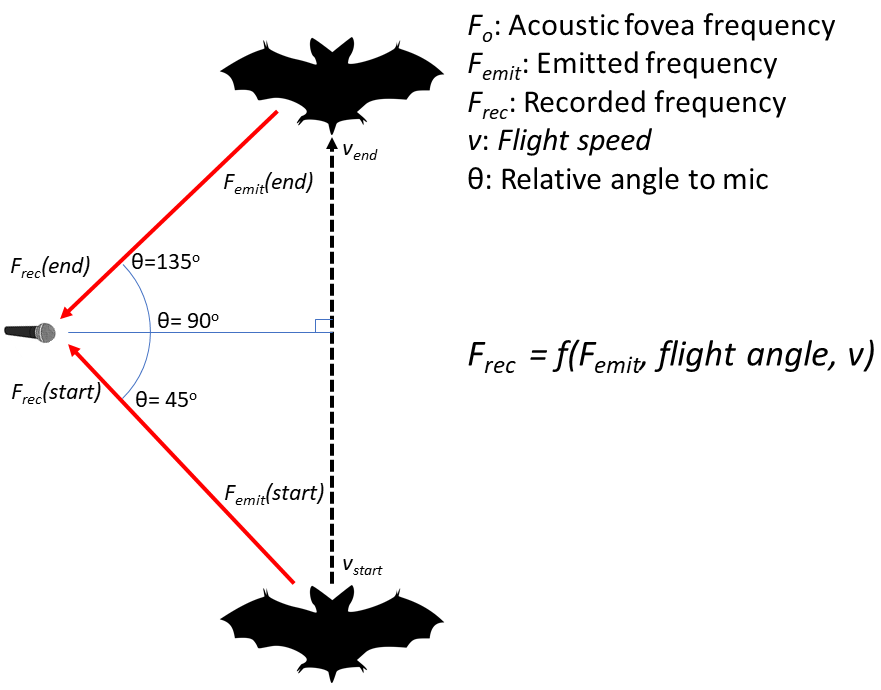
\includegraphics[width=1\linewidth]{original_papers/hbc-paper/figures/doppler_shift_schematic} \caption{Schematic showing the simple model used to calculate the expected dominant frequency variation arising from a single bat flying past the microphone. $F_{e}$ is the doppler compensated emitted frequency. $F_{rec \:start}$ is the received frequency at the start of the flight, $F_{rec \:end}$ the received frequency at the end of the flight. $v_{start}$ and $v_{end}$ are the speed of the bat at the start and end of the flight. $F_{rec}$ is a function of the emitted frequency, relative flight angle and flight speed at the start and end of the fly by.}\label{fig:dopplerschematic}
\end{figure}

Our simulations recreated the frequency recorded at the micrphone at the `start' and `end' of the bat's flight past the microphone (Figure \ref{fig:dopplerschematic}). The start position was assumed to be 45 degrees and end position was 135 degrees relative to the microphone (where 90 deg. corresponds to the bat flying exactly perpendicular to the microphone's direction). The speed at the start and end flight positions of the bat was assumed to be between 1.5-4.5 m/s, and the acoustic fovea's of the bat population was assumed to be between 100-111 kHz, matching the range of the study species' \emph{R. euryale/mehelyi}. The frequency recorded at the microphone due to Doppler shift from the bat flying at an angle was calculated by: \(\frac{v_{sound}}{v_{sound}-v_{bat}cos(\theta)}\). The bat's Doppler shift compensation was modelled by assuming the bat perfectly compensated for Doppler shift due to it's own flight speed. The \(F_{e}\) was calculated at the start and end points as \(F_{e}=\frac{F_{o}}{\frac{v_{sound}+v_{bat}}{v_{sound}-v_{bat}}}\), where \(v_{bat}\) depended on the flight speed at the start and end points, \(v_{sound}=330\)m/s, and \(F_{o}\) was a randomly chosen value between 100-111 kHz.The DF range was calculated as \(DF_{range}=abs(F_{rec\:start}-F_{rec\:end})\). Figure \ref{fig:singledomfreqrangesim} shows that our the DF ranges from simulations match the observed DF ranges well for the single bat case.

\begin{figure}
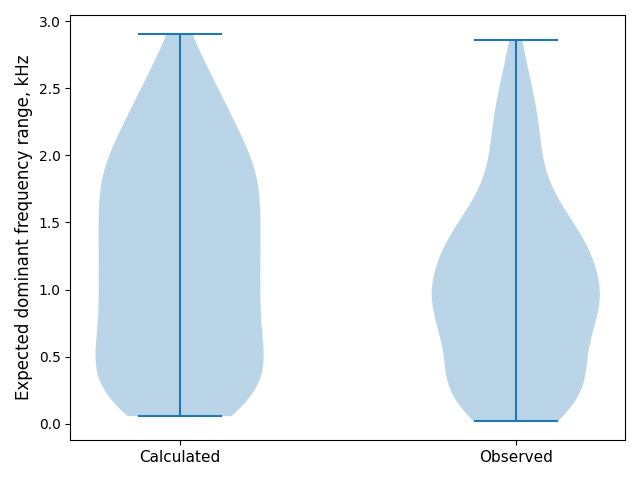
\includegraphics[width=1\linewidth]{original_papers/hbc-paper/combined_analysis/domfreq_range_single} \caption{\label{fig:singledomfreqrangesim} Calculated (left) and observed (right) dominant frequency range for a single bat flying past the microphone. The calculated and observed ranges match fairly well, indicating the broad processes behind the observed  dominant frequency range have been captured.}\label{fig:singledomfreqrangesim}
\end{figure}

When two or more bats echolocate in the same volume, it is expected that the DF range will increase because of the unique acoustic fovea's each bat has. What is the range of expected range increase when the two bats echolocate independently however? To understand the expected DF range when multiple bats are flying we simulated the case of two bats echolocating independently in the same volume. The acoustic fovea of both bats was randomly chosen, and so were their start and end speeds. The DF range for the two bat case was thus calculated over a series of 1,000 random parameter combinations to reveal the range of dominant frequency ranges expected in two bat cases. In the two bat case, \(DF_{range}=max(F_{rec})-min(F_{rec})\) without reference to when or which bat emitted the call.

Figure \ref{fig:multidomfreqsim} shows the dominant frequency ranges expected from single and a pair of bats. The median difference of the multi-single DF ranges is expected to be around 3.9 kHz, even though there is a wide variation in the observed DF ranges. The experimentally observed multi-single DF range difference of \textasciitilde2 kHz falls within the range difference shown in Figure \ref{fig:multidomfreqsim}, however more detailed parametrisation of the flight speeds and relative positions may lead to a better match of the observed data.

\begin{figure}
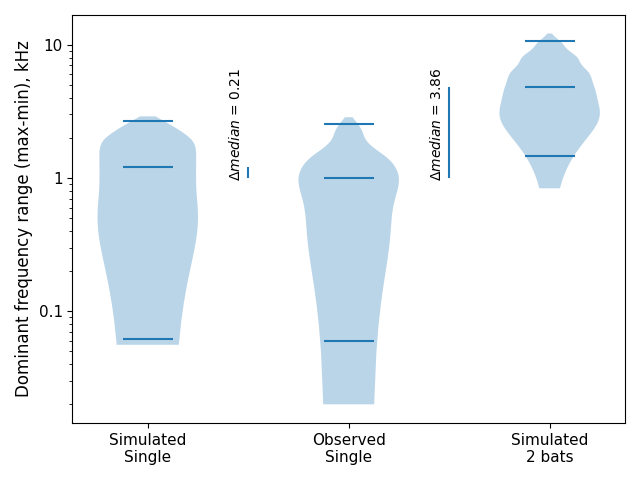
\includegraphics[width=1\linewidth]{original_papers/hbc-paper/combined_analysis/domfreqrange_singlemultisim} \caption{\label{fig:multidomfreqsim} The distribution of dominant frequency ranges expected when a single bat echolocates (left), observed when a single bat (middle), and calculated when two bats fly.}\label{fig:multidomfreqsim}
\end{figure}

The code to implement this calculation is in the \texttt{Combined\ analysis\ notebook.ipynb} and its HTML version.

\hypertarget{simtfmoverlap}{%
\section{tFM echo-call overlap probabilities}\label{simtfmoverlap}}

The probability of a tFM echo overlapping with the tFM portion of another bat's call was derived through simulation. The echo/call duration was fixed at 3.4ms and the inter-tFM duration was set to 40 and 50ms. A tFM echo was placed randomly in a time-span between 0-(echo + inter-tFM duration). A tFM call was also randomly placed in the same time-span, and a temporal overlap was checked. The random placement and overlap checking was done 20,000 times to derive a probability of echo-call overlap at the two inter-tFM intervals.

For \emph{3} bats, an echo may be overlapped by two calls. The probability of echo-call overlap here is between 1.6 to 2.1\%. Further details are in the Jupyter notebook titled \texttt{tFM-overlaps.ipynb}.

\hypertarget{ushichkachapter}{%
\chapter{\texorpdfstring{The \emph{Ushichka} dataset: a multi-channel, multi-sensor dataset to unravel active sensing in groups}{The Ushichka dataset: a multi-channel, multi-sensor dataset to unravel active sensing in groups}}\label{ushichkachapter}}

\chaptermark{The Uschichka dataset}

\newpage

\hypertarget{ushichka_abstract}{%
\section*{Abstract}\label{ushichka_abstract}}
\addcontentsline{toc}{section}{Abstract}

The collective behaviour and motion of animal groups has been intensely investigated. The behavioural heuristics underlying the impressive acts of self-organisation have been revealed through a combination of experimental tracking and modelling. More specifically, visually driven animal collectives such as fish and mammals have been the focus of studies. Visually driven collective behaviours scale well with group size given sufficient ambient light. In contrast to passive sensing animals, active sensing animals like echolocating bats emit probes of energy to detect their surroundings. Echolocating bats emit loud ultrasonic calls and listen for faint returning echoes to detect objects. When multiple bats echolocate together however, it is expected that they will not be able to detect their surroundings well due to masking. This masking means that collective behaviour in active sensing bats is not expected to scale well with group size. However, despite this expectation, bats aggregate and fly together in large groups during cave emergences and mating swarms. The sensory and behavioural heuristics behind these formations remain understudied to date. The study of group echolocation has also been impeded by technological issues in experimental tracking, analysis of recordings with high call densities, and a deficiency of parametrised computational models. To fill these gaps in the study of active sensing groups, we present the \emph{Ushichka} dataset. \emph{Ushichka} is a multi-channel, multi-sensor dataset consisting of audio and video data of bats echolocating as they fly in a cave. A LiDAR scan of the recording volume is also part of the dataset. \emph{Ushichka} promises to generate a detailed spatio-temporal understanding of how bats in groups deal with the problem of masking as they echolocate together in close proximity. The dataset is, to our knowledge, one of its kind in capturing bat collective behaviour with multiple sensors, and promises novel insights into the sensorimotor heuristics of active sensing groups. While promising novel insights, \emph{Uschichka} also presents a series of technical challenges ripe for inter-disciplinary collaborations such as LiDAR-thermal camera alignment, multi-channel call correspondence matching and automatic microphone position estimation. The processed dataset will consist of individual level trajectory and call information that are aligned to the LiDAR scan of the cave. This processed dataset can be used to parametrise existing models of collective behaviour, compare behavioural heuristics with group size, and to reconstruct the auditory scene of each bat in the group.

\newpage

\hypertarget{introduction-2}{%
\section{Introduction}\label{introduction-2}}

Many animals across the tree of life move and live in groups, and show impressive coordinated behaviours \citep{sumpter2006principles}. Coordinated behaviours shown in these collectives are reproduced by simple heuristics in models with agents responding independently to the movement and positions of their neighbours \citep{couzin2002a}. These coordinated behaviours have been well investigated in visually dominant animal collectives such as birds, mammals and fish \citep{ballerini2008a, strandburg2013visual, pita2016collective}. Vision is a `passive' sensory modality, in that the animal acts solely as a receiver of light \citep{nelson2006a}. Visually driven collective behaviour can thus scale well with group size, given sufficient ambient light.

In contrast to passive sensing animals, are `active' sensing animals. Active sensing animals (sensu stricto \citet{nelson2006a}), such as bats, dolphins and electric fish, emit probes of energy and monitor the modulation of the probes by the environment around them . Echolocating bats emit loud ultrasonic calls, and listen to the returning echoes to detect objects around them \citep{Griffin1958}. When multiple echolocating bats echolocate together, they can start to negatively affect each other's ability to detect their own echoes \citep{ulanovsky2008bat}. Every bat emits loud calls, and is attempting to listen to its own echo. However, along with its own returning echoes, each bat hears loud `non-target' sounds (calls and echoes of neighbouring bats) which hamper its own echo detection. A bat that cannot detect its own echoes is metaphorically `flying blind', and risks colliding into its neighbours, and of more concern, into hard structures around it. As the number of bats in a group increases, the number of non-target sounds increases rapidly in a non-linear fashion (\textasciitilde{}\((N_{bats}-1)^2\)). Sensory simulations show that in large groups of bats, a bat may be detecting its neighbours every few calls - and not every time it emits a call \citep{beleyur2019modeling}. Despite the expected deterioration of echolocation with increasing group sizes, echolocating bats in nature are social and form very large aggregations in the form of mating swarms, cave roosts and evening emergences \citep{Ortega2016, Erkert1982, gillam2010tbrasiliensis}. The dynamics of active sensing groups is understudied \citep[but see][]{theriault2010a}, and perhaps likely to differ from passive sensing groups in one respect. Given sufficient light, an animal in a visually driven collective will be able to detect all neighbours in its vicinity even at large group sizes. In contrast, the number of neighbours potentially detected by a bat in a group decreases with group size \citep{beleyur2019modeling}, leading to a limited sensing ability. While it is parsimonius to assume that existing computational models may be able to capture the dynamics of sensorially limited active sensing groups (through models with `limited interactions' sensu \citep{bode2011a}), it remains to be experimentally seen in what respects the behaviour of active sensing groups differ from the visually driven animal collectives studied so far. Even if active sensing groups do indeed behave much like visually driven passive sensing groups, experimental confirmation remains lacking to date.

Here we present the conceptual motivation and technical equipment behind the \emph{Ushichka} dataset. The word Ushichka (Ушичка, \emph{OO-shi-ch-kaa}) in Bulgarian has a dimunutive connotation for something with multiple ears. The name is chosen to highlight the fact that \emph{Ushichka} is a multichannel, multi-sensor dataset which aims to unobtrusively `listen' (observe with technological eyes and ears) to groups of multiple bats echolocating in the wild. The \emph{Ushichka} dataset is, to our knowledge, a unique dataset in that it comprises of multichannel audio and video datasets of bats echolocating in groups in their \emph{natural environment} captured by a LiDAR scan of the space. The multichannel nature of the dataset allows 3D localisation and tracking with high spatio-temporal resolution. Previous experimental work on multi-bat echolocation in the lab and field to date has mostly been with upto 2 bats a time \citep{goetze2016a, giuggioli2015a, necknig2011between, fawcett2015clutter, fawcett2015echolocation}, or multichannel data of solely video or audio \citep{theriault2010a, lin2016bats}. The multi-camera, multi-mic nature of \emph{Ushichka} allows us to explore echolocation in groups in much greater detail than previously attempted.

\hypertarget{the-experimental-study-of-echolocating-bat-groups}{%
\subsection{The experimental study of echolocating bat groups}\label{the-experimental-study-of-echolocating-bat-groups}}

The study of bat echolocation has a long and grand history dating back over 200 years, first documented in Spallanzi's experiments in the 18th century.
After the formal discovery of echolocation \citep{Griffin1958, Dijkgraaf1946}, the field has moved leaps and bounds. A detailed understanding of the physiology, behaviour, neurobiology and acoustics behind echolocation has been uncovered in great detail \citep{popper1995hearing, Fenton2016}. While a large body of knowledge is in place about how \emph{individual bats} are able to echolocate through the use of trained animals in laboratory settings and field observations \citep{Fenton2016}, comparitively little is known on how they echolocate in groups\citep{ulanovsky2008bat}.

Previously, the challenges in echolocation fieldwork included bulky analog recording and signal analysis equipment; limiting the speed and quantity of data that could be collected, and analysed \citep{Griffin1958, habersetzer1981a}. The onset of the digital revolution has allowed for lightweight devices that can collect more data, which can then be analysed more easily. Current experimental approaches to study echolocation in groups include, for example, on-body tags that record audio from the focal animal and its neighbours (along with GPS and accelerometer data)\citep{cvikel2015b}, microphone-camera pairs to quantify broad echolocation characteristics with group size \citep{lin2016bats} and thermal camera 3D tracking with sophisticated computer vision to track individuals in the million-strong emergence behaviour of \emph{Tadarida brasiliensis} \citep{betke2007tracking, theriault2010a}. Each of these studies has provided exciting and important insights into how echolocating bats manage to echolocate in groups. For instance, \citet{cvikel2015b} showed that \emph{Rhinopoma hardwickei} do not seem to show the `jamming avoidance response' (shifting call frequencies to avoid overlap with neighbours, sensu \citet{ulanovsky2004dynamics}) first seen by \citet{habersetzer1981a}. \citet{lin2016bats} find that bats echolocating in caves actually increase their pulse rate with group size, in contrast to theoretical expectations and results from another species that decreases its pulse rate \citep{jarvis2013groups}. \citet{theriault2010a} advanced the field by quantifying the geometry of a \emph{T. brasiliensis} emergence, showing that animals in larger groups fly relatively close to each other (0.5m), and that neighbours are placed uniformly across azimuth and elevation around individuals, unlike that seen in bird flocks \citep{ballerini2008a}. In starling flocks for instance, neighbours are located non-uniformly in the elevation and azimuth in that they are less likely to be found in front or behind a focal individual.

\emph{Ushichka} represents a natural and quantitative step forward to all the recent work in the study of group echolocation in the field. The one important respect where \emph{Ushichka} differs from previous work is its inherent `multi-modality', in that it consists of simultaneously captured multi-microphone, multi-camera data streams, along with 3D scans of the recording volume for physical context. On-body tags and single microphone recordings lack explicit information of how many or where neighbours were located. Pure video tracking with one or more cameras does not provide insights into the echolocation behaviour of animals across group sizes. \emph{Ushichka} captures flight and echolocation data of the group, and holds promise to provide access to the auditory scene \citep{Moss2001} of each individual in the group. Reconstructing the sensory inputs of individuals in a group allows us to better understand the sensorimotor decisions animals make \citep{strandburg2013visual}. While an established method in visually driven animal groups like fish, auditory scene reconstruction is an exciting new frontier for the field of group echolocation, that \emph{Ushichka} promises to provide.

\hypertarget{experimental-methods}{%
\section{Experimental methods}\label{experimental-methods}}

\hypertarget{field-site-and-study-species}{%
\subsection{Field site and study species}\label{field-site-and-study-species}}

Recordings of wild echolocating bats were made in the Orlova Chuka cave system (Ruse, Bulgaria). Recordings were made of bat flight and echolocation in the chamber first encountered after the entry corridor (Figure \ref{fig:cavesetup}, \ref{fig:othercavesetup}). Recordings were conducted in the recording volume (\emph{w x l x h}\textasciitilde5x9x3 m\(^{3}\)) between 19th June to 19th August 2018 over the course of 14 recording sessions (Suplementary Information (SI): Table \ref{tab:nightandplayback}). One recording session typically started around sunset and ended around sunrise the next day (See \ref{recschedule}).

Orlova Chuka is known to host at least 9 species of bats \citep{Ivanova2005, govtbatcount}. During the summer, resident \emph{Myotis myotis} and \emph{Myotis blythii} females form the dominant bat population. These female bats arrive in spring and spend the summer in the cave system raising their young. Though rigorous mark-recapture data is missing, individual mothers are known to be consistent in returning to the cave system over multiple nights (pers. comm., Laura Stidsholt, Stefan Greif). Given the dominance of \emph{Myotis myotis} and \emph{Myotis blythii} (hereon referred to as \emph{M. myotis/blythii}) in the cave system, it can be fairly said that the \emph{Ushichka} dataset consists mainly of these two species. The calls of \emph{M. myotis} and \emph{M. blythii} are indistinguishable (their morphology is also extremely similar too) \citep{dietz2016bats}. Due to the great similarity in their echolocation calls, they are treated as one group of bats. The frequency ranges of \emph{M. myotis/blythii} are lower than those of the other resident frequency modulating bats in the cave (eg. \emph{M. daubentonii, M. capacinii, Miniopterus schreibersii}) and are very easily distinguishable from the rhinolophid bats (\emph{Rhinolophus ferrumequinum, R.euryale, R. mehelyi})\citep{dietz2016bats}.

\begin{figure}
\centering
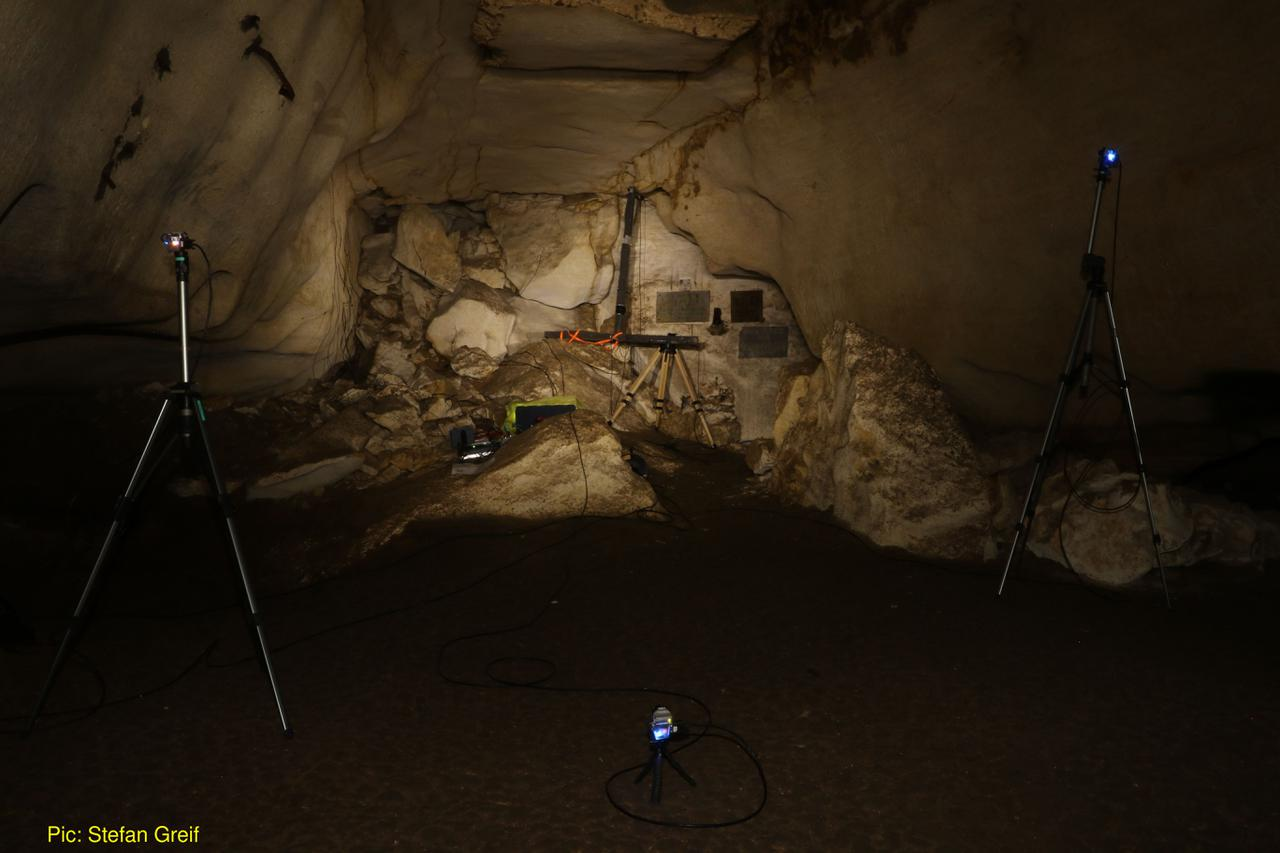
\includegraphics{original_papers/ushichka-figures/ushichka_setup_DC6A5930_w.JPG}
\caption{\label{fig:cavesetup}The \emph{Ushichka} setup. The large inverted T shaped array in the centre of the image is the 120cm tristar array with four SANKEN CO-100 microphones. The three blue lights are from the three thermal cameras pointing towards the array. The rest of the microphones are smaller Knowles SPU 0410 units are attached to the wall on the left portion of the image and are not visible.}
\end{figure}

\begin{figure}
\centering
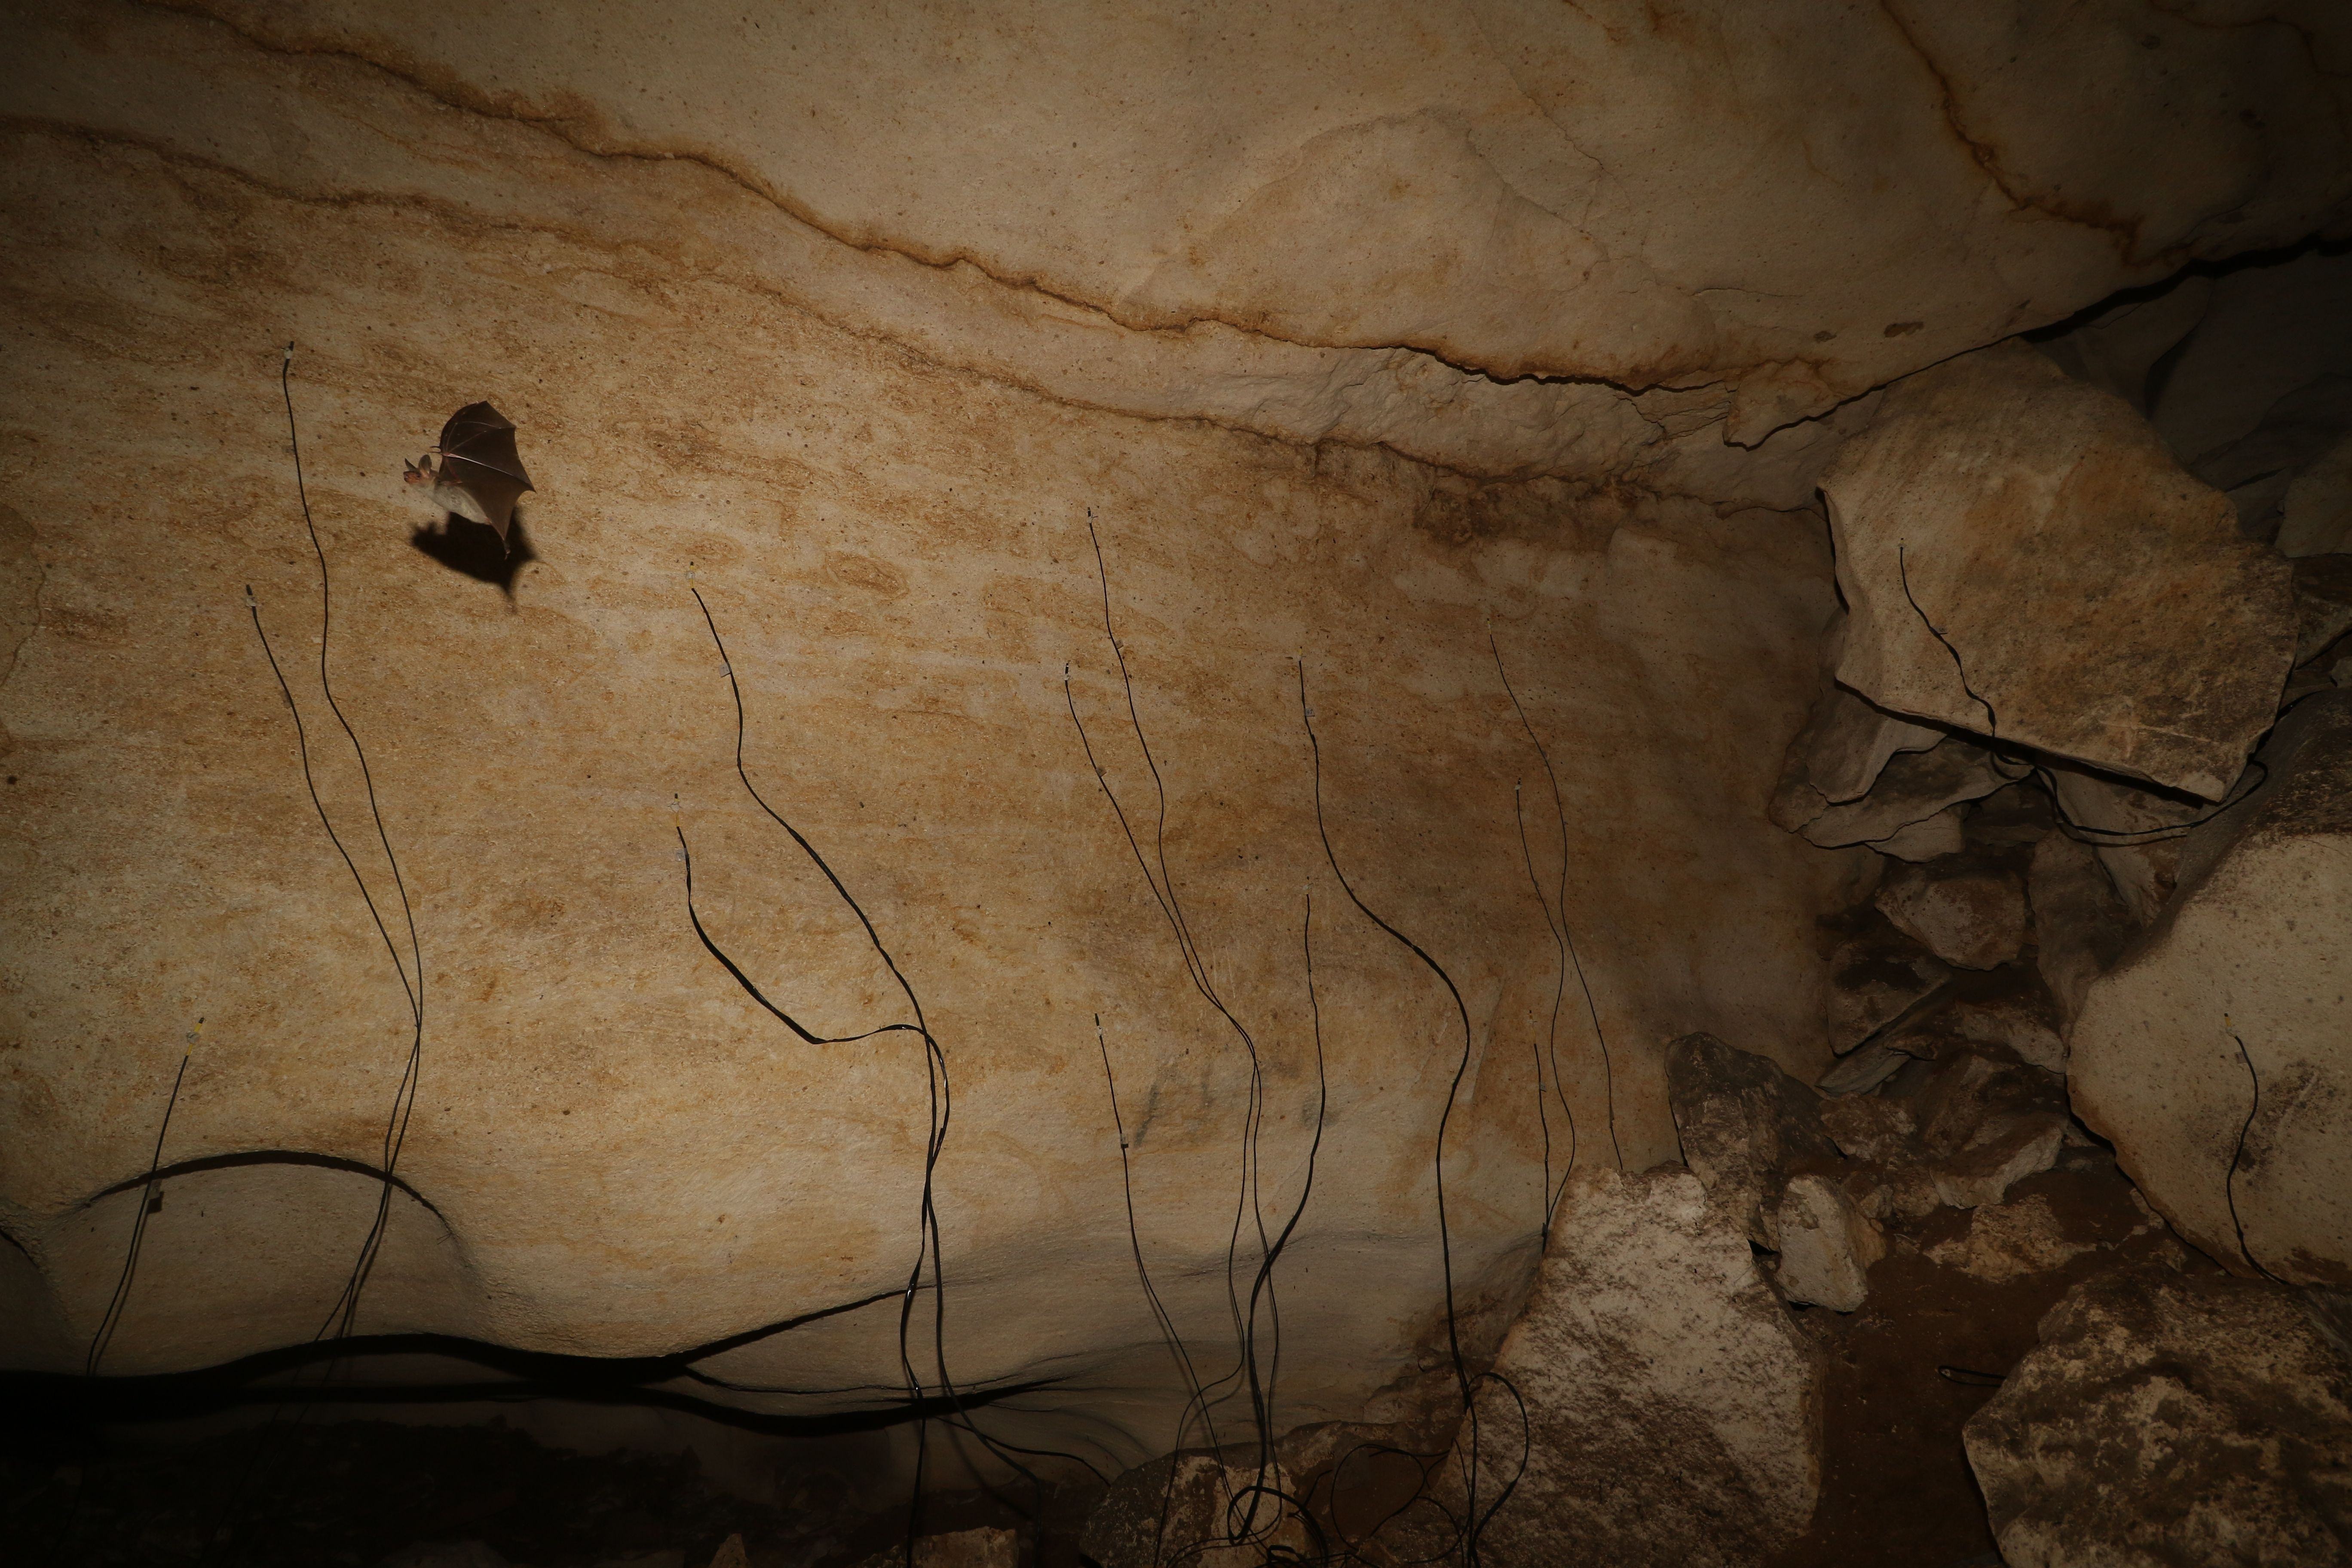
\includegraphics{original_papers/ushichka-figures/DC6A6061.JPG}
\caption{\label{fig:othercavesetup}The \emph{Ushichka} setup with the smaller Knowles SPU microphones on the wall referred to in Figure \ref{fig:cavesetup}. In the picture is a \emph{M. myotis/blythii} bat flying past the array. Photo by Stefan Greif.}
\end{figure}

\hypertarget{audio-video-and-lidar-systems}{%
\subsection{Audio, video and LiDAR systems}\label{audio-video-and-lidar-systems}}

\hypertarget{audio}{%
\subsubsection{Audio}\label{audio}}

Multichannel audio data was recorded by multiple (2-3) Fireface (RME GmbH, Germany) sound cards running at 192kHz connected to a laptop (DELL Latitude E6540, Windows 7 enterprise, core i5, 16GB RAM). The laptop was verified not to emit ultrasound. All sound cards were Fireface USB type, ASIO protocol based soundcards. The number of channels of audio in the \emph{Ushichka} dataset varied between 12-22 channels over the course of the field season. The 12-22 channel data consisted of four SANKEN CO-100 microphones with the rest of the 8-18 channels coming from Knowles SPU-0410 microphones. All microphones were connected to either the inbuilt pre-amplifiers of the sound cards, or to two RME QuadMic II (RME GmbH, Germany) pre-amplfiers. Later recordings with the \emph{Ushichka} setup also included a Focusrite Scarlett OctoPre (Focusrite Plc, UK) pre-amplifier.

All recording nights had a 4-channel 120cm tristar mounted in a fairly constant position in front of the memorial plaque in the recording volume. A `tristar' array is a common planar array configuration \citep{Hugel2017, Goerlitz2010, Lewanzik2018}, with three microphones placed at a fixed radius from a central microphone. The three peripheral microphones are separated from each other by a 120 degree angular separation. The entire set of four microphones is accomodated on an inverted T-shaped metal array. The Knowles SPU-0410 microphones were spread around the recording volume to increase the variety of locations at which bat calls were recorded. The positions of microphone were constant within a recording session, and were often changed between sessions. On a few occasions, the microphones were kept in the same position across consecutive recording nights. Microphones were not left in the cave across multiple days due to concerns of humidity affecting the electronic circuits and membranes, especially of moisture build up in the Knowles SPU 0410 recording inlet.

A subset of all possible inter-mic distances were measured every recording session using a GLM 50C (Bosch, Germany with 1mm accuracy) laser range finder. Ultrasonic sweeps were played back from multiple points in the recording volume as part of an automatic mic position estimation workflow. Most of the microphones were calibrated for their frequency response and directionality at least once after the field season. For more information on the microphone automatic position estimation and calibrations please refer to the SI (\ref{ushichkasi}).

\hypertarget{video}{%
\subsubsection{Video}\label{video}}

Three thermal cameras (9mm focal length, TeAx ThermalCapture 2.0, TeAx Technology GmbH, Germany) running with FLIR Tau 640 cores (640x512 pixel image resolution, FLIR, USA) at 25Hz formed the camera array. All three cameras (Figure \ref{fig:multicambats}) were frame synchronised in their video recording. There were a few occasions where one or two cameras recorded an extra frame, and these extra frames are known from previous tests to be at the end of the recording, and not jitter in recording initiation.

\begin{figure}
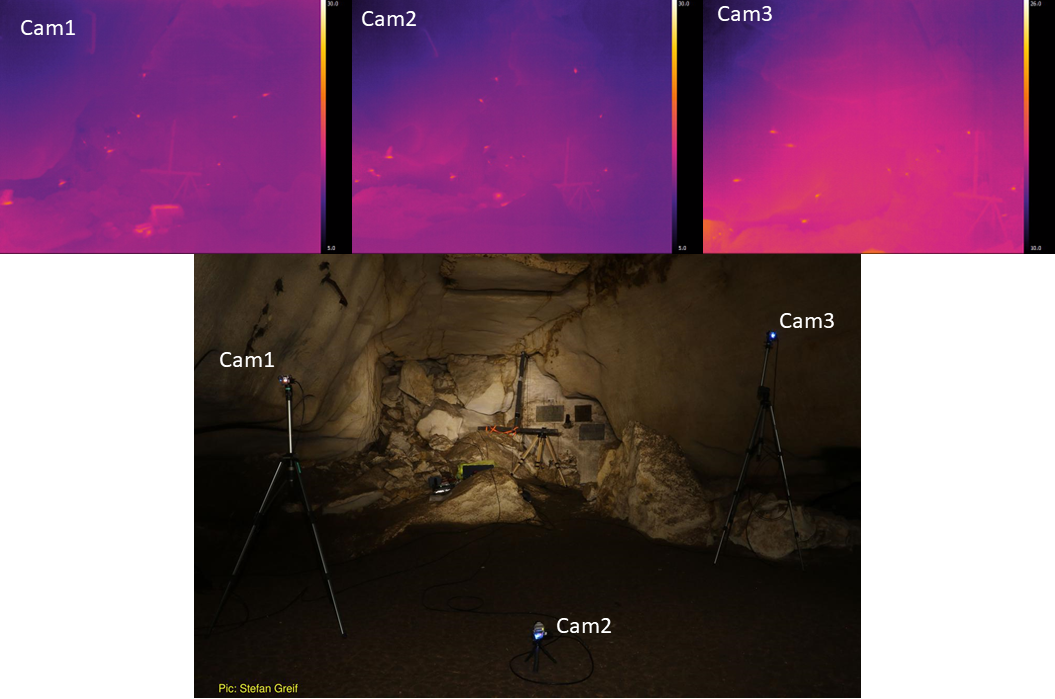
\includegraphics[width=1\linewidth]{original_papers/ushichka-figures/multicam_views} \caption{\label{fig:multicambats}A multi-camera view of bats flying in the recording volume, allowing 3D tracking of flying bats (from the frame-synchronised thermal video recordings).}\label{fig:multicambats}
\end{figure}

The microSD cards (SAMSUNG PRO+, 32 GB) were inserted into each camera at the start of each recording session. Removing the microSD card from the cameras required significant disturbance of their position, and thus the total video recording time was limited by the one-time microSD card memory capacity. The location of the microSD cards \emph{inside} the camera housing meant that the data from the cameras could only be transferred in the morning after the end of the recording session. All cameras were calibrated using the `wand' protocol described in \citet{Theriault2014}. Further details on camera intrinsic and extrinsic parameter calibrations, wand setup, and synchronisation with audio are in the SI \ref{ushichkacamcalib}.

\hypertarget{lidar}{%
\subsubsection{LiDAR}\label{lidar}}

A LiDAR scan of the recording volume provides a physical context to place the observed echolocation and flight behaviour of the bats. With only the audio and video data, we will at most be able to recreate the positions and time of call emissions of the bats themselves. While bats are likely reacting to each other's presence, they will also be reacting to the presence or absence of physical obstructions such as cave walls. With the LiDAR scan for example, we will be able to understand if a change in trajectory or call behaviour arose from the bats' proximity to the cave wall, or to its nearest neighbour.

A LiDAR scan of the recording volume, along with a large portion of the Orlova Chuka cave was carried out in collaboration with Dr.~Asparuh Kamburov (University of Mining and Geology ``St.~Ivan Rilski'', Sofia). The LiDAR scan provides a high spatial resolution (\textless1cm) 3D map of the cave's surface and objects in it (Figure \ref{fig:lidarimage}). The details of the LiDAR scanning, data processing and description can be found in \citet{bggeospatial}.

\begin{figure}
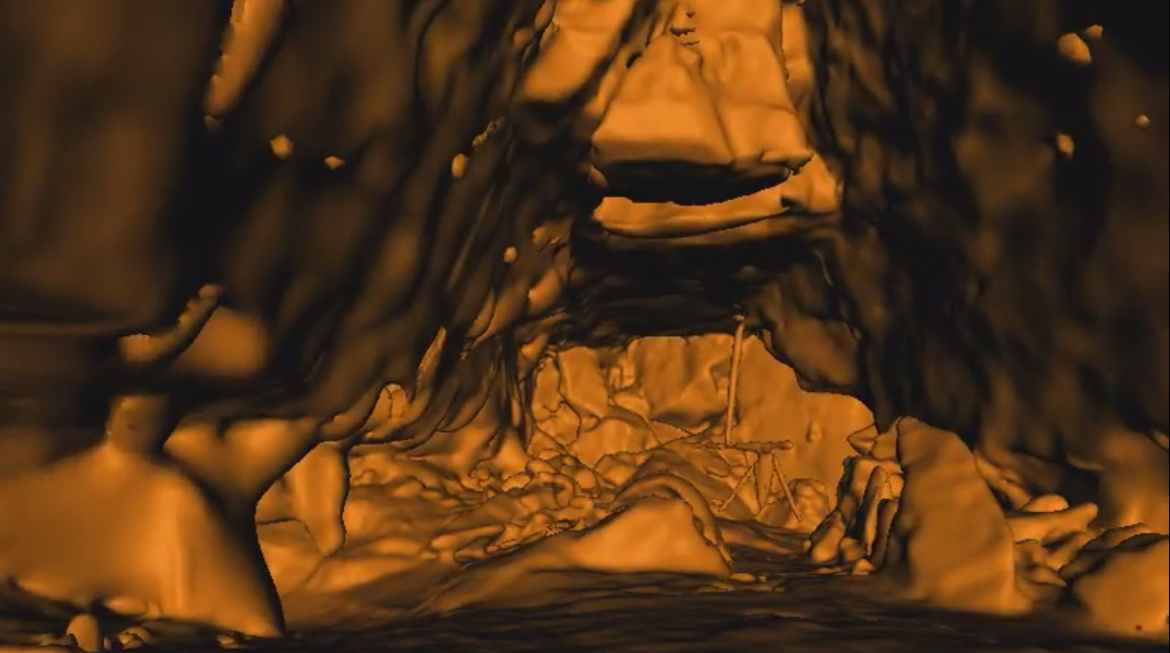
\includegraphics[width=1\linewidth]{original_papers/ushichka-figures/lidar_image} \caption{The LiDAR map of the recording volume showing the same view as in Figure \\ref{fig:multicambats}, with the large tristar array.}\label{fig:lidarimage}
\end{figure}

\hypertarget{weather-data}{%
\subsubsection{Weather data}\label{weather-data}}

The local weather conditions (humidity, temperature and atmospheric pressure) within the cave were recorded by a Kestrel 4000 weather meter (Nielsen-Kellerman, USA) placed in the recording volume. The logged weather variables play a role in the accuracy of positioning and source level estimates \citep{goerlitz2018weather, lawrence1982measurements}, and were thus measured to later estimate the speed of sound and absorption of ultrasonic sound more accurately across recording sessions.

\hypertarget{recschedule}{%
\subsection{Recording schedule}\label{recschedule}}

The audio and video arrays were mostly setup before sunset (\textasciitilde21:00 Eastern European Time) and collected data till around sunrise (\textasciitilde5:30 EET) with one break in between. The recording break between around 12-3 am co-incided with an observed drop in bat activity around midnight.

Recordings were triggered manually in 2 of 14 recording sessions in response to bat calls heard on a bat detector (SI Table \ref{tab:recnights}). For the rest of the sessions, recordings were triggered automatically. A recording was automatically triggered by bat calls that went above a threshold rms level across a subset of monitor channels (between -50 to -40 dB, threshold adjusted across recording sessions). Once triggered, the recording was set to stop after a pre-defined duration. There were no other sources of ultrasonic sound in the cave, and it can be said with great certainty that all recordings were triggered only by bat calls. Each recording in the \emph{Ushichka} dataset consists of 10-15 second long audio-video file pairs (See SI \ref{ushichkaavmatch} for details of audio-video synchronisation). The variation in recording duration is due to adjustments made over the course of the field season.

Bats can emit over 10 calls per second, which would lead to an almost continuously triggered recording system. While technically feasible, continuous recording of data would lead to unmanageably large files. Moreover, the TeAX thermal cameras relied on high speed microSD cards that were the limiting factor in the amount of data (32 GB) that could be collected over the course of one recording session. The audio-video recording system was thus set to record at a fixed duty cycle of around 20\% across sessions. For example, a 20\% duty cycle and 10 second recording duration meant that recordings could be triggered at most every 50 seconds (10s recording + 40s inactivity).

\begin{figure}
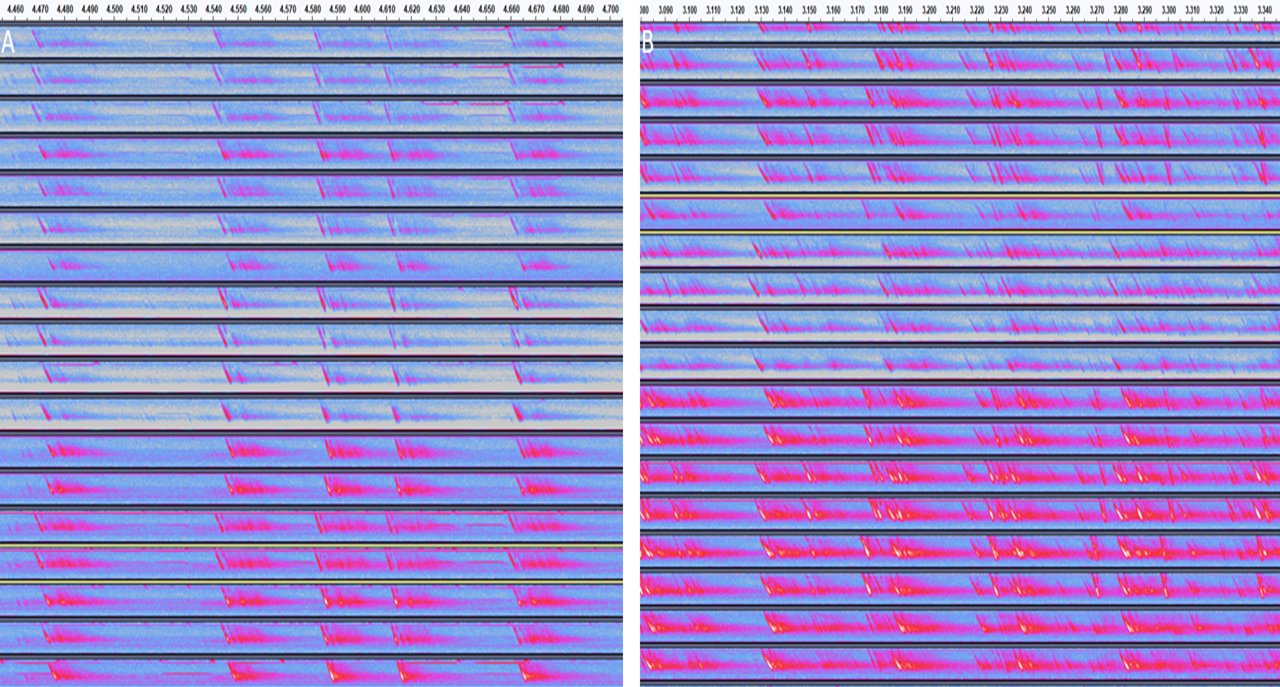
\includegraphics[width=1\linewidth,height=0.5\textheight]{original_papers/ushichka-figures/multichannel_composite_elongated} \caption{Spectrograms showing a subset channels from the multichannel audio data collected. The spectrograms show highlight some of the challenges of working with the audio data including reverberation, multi-path propagation, call overlaps, and correct call identity matching across channels. A) an example of a recording with a few bats in it B) recording with multiple bats in it.}\label{fig:multichannel-calls}
\end{figure}

There are a few occasions of skipped morning and evening recordings due to various technical and logistical issues that were encountered over the course of the field season.

\hypertarget{bat-activity}{%
\subsection{Bat activity}\label{bat-activity}}

Bats began to fly from the interior roosting sites into the recording volume around the time of sunset. The initial activity is typically due to small groups (2-5) of \emph{R.euryale} and \emph{R. mehelyi} flying rapidly and unpredictably in the volume. The activity of the rhinolophid bats seemed to reduce with time, and gave way to a slowly rising number of \emph{M. myotis/blythii} bats. The number of bats flying in the recording volume could be as high as thirty bats at a time. Towards end June, it was noticed that the \emph{M. myotis/blythii} bats also formed temporary roosting clusters on the walls of the recording volume, and this behaviour seemed to decrease in its frequency as the season progressed. Cloudy and rainy evenings lead to a delay or complete absence of emergence from the cave.

Peak bat activity in the recording volume was typically seen about 1-1.5 hours after sun-set. The bats then began to exit the cave (Figure \ref{fig:activity}). The exit seemed relatively rapid, after which only a few bats were seen to still fly in the recording volume. Individual bats returned in the early morning from one to two hours before sunrise onwards. It seemed that \emph{R. euryale} and \emph{R. mehelyi} activity remained fairly constant through the night, even during the drop in activity around midnight.

\begin{figure}
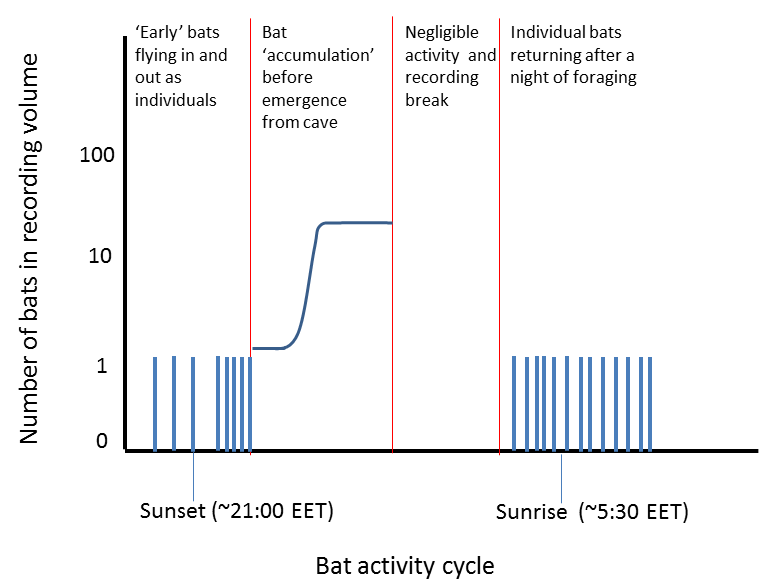
\includegraphics[width=1\linewidth]{original_papers/ushichka-figures/ushichka_activity} \caption{Schematic of typical bat activity pattern of Myotis myotis and Myotis blythii between sunset to sunrise in the *Ushichka* dataset. The multichannel recording system was typically activated before sunset and was run till after sunrise with a break in between.}\label{fig:activity}
\end{figure}

\hypertarget{software-used-in-this-work}{%
\subsection{Software used in this work}\label{software-used-in-this-work}}

Automatic recording triggering implemented in the \texttt{fieldrecorder\_trigger} module relies on the open-source Python language \citep{van2011python}, and the sounddevice, scipy and numpy \citep{geier2015a, virtanen2019a, oliphant2006a} packages. This manuscript was written using the knitr package \citep{knitr}.

\hypertarget{technical-challenges-ahead-and-potential-solutions-in-analysing-the-ushichka-dataset}{%
\section{\texorpdfstring{Technical challenges ahead and potential solutions in analysing the \emph{Ushichka} dataset}{Technical challenges ahead and potential solutions in analysing the Ushichka dataset}}\label{technical-challenges-ahead-and-potential-solutions-in-analysing-the-ushichka-dataset}}

Analysing the echolocation call data in \emph{Uschichka} will require surmounting a series of challenges, here discussed in increasing order of difficulty.

\begin{enumerate}
\def\labelenumi{\arabic{enumi})}
\item
  Reflections : The recording volume consisted of acoustically reflective surfaces, leading to significant reverberation and multi-path propagation. Dealing with reverberation is likely to be relatively straightforward while performing acoustic tracking, as cross-channel correlations should be able to filter out the noise contributed by reverberation. Multi-path propagation, where a sound arrives multiple times at each microphone due to distinct reflections is likely to be a somewhat more difficult problem to deal with, especially considering that if a single call leads to \emph{N} multi-path reflections, then \emph{M} calls in the volume could then lead to \emph{NxM} reflections.
\item
  Call density : Each bat flying in and out of the volume emits calls 10-20 times per second (10-20 Hz call rate). With one bat, it is relatively straightforward to acoustically localise the bat as calls are separated by tens of milliseconds. With an increasing number of bats in the volume, (as happens towards the end of the night, Figure \ref{fig:activity}), the temporal separation between calls will decrease, and also lead to a higher occurence of call overlaps. Handling such high call densities will be a challenge, and require the latest techniques in call detection in the presence of overlaps \citep{izadi2020separation}, or in general blind signal separation techniques \citep{brandstein2013microphone}.
\item
  Correspondence matching : Even if calls can be detected reliably in single channels, the problem of cross-channel correspondence still remains to be solved, a common problem faced in any multi-channel acoustic array \citep{brandstein2013microphone}. An echolocation call detected in one channel needs to be matched with itself in another channel, despite the possible presence of multiple similar calls in the expected time-window. Individual bats do have unique call characteristics (\citet{masters1995sonar}, and in \emph{M. myotis}: \citet{yovel2009voice}; but also see \citet{siemersnovoice}). The unique echolocation call `signatures' are sometimes apparent from visual inspection of the spectrogram. However, manual correspondence matching is unlikely to scale well in terms of effort required with group sizes beyond 3 bats and will require robust automated algorithms to solve this problem.
\end{enumerate}

One important `support system' which may help significantly in solving the issues of multi-path propagation and correspondence matching is the multi-camera video data. Each call is emitted from one position by a bat, and captured on multiple audio channels. The time-synchronised 3D video tracking data contains the microphone positions and bat trajectories. With this in mind, we can combine the audio and video tracking to simplify cross-channel correspondence matching and the process of assigning a call to its source bat. The basic principle of acoustic localisation relies on the fact that with at least 4 microphones spread in space, each position of sound emission will generate a unique set of time-differences-of-arrival (TDOA). A TDOA in a microphone array is the difference in arrival times of a sound in comparison to a chosen reference channel. Measuring these TDOAs allows inferring the position at which a bat emitted a call from. The 3D video trajectories allow the generation of a series of `hypotheses' of which calls could have been emitted at which point in space. By calculating the time-varying distances between a bat and each microphone across time, it will allow us to generate a set of `predicted' TDOAs that calls could be arriving at. The problem thus boils down to a matching problem, where all TDOAs from all possible call correspondence matches are filtered based on which TDOAs are predictions from a given flight trajectory. The video trajectory based filtering approach could in principle elegantly solve the problems of multi-path propagation and cross-channel correspondence at one shot. However, whether the 3D video data will actually be able to deliver sufficiently accurate position estimates, and thus accurate TDOAs remains to be seen.

\hypertarget{fusing-multiple-data-streams-to-reconstruct-individual-auditory-scenes}{%
\subsection{Fusing multiple data streams to reconstruct individual auditory scenes}\label{fusing-multiple-data-streams-to-reconstruct-individual-auditory-scenes}}

Reconstructing individual auditory scenes requires a recreating the incoming sounds heard and outgoing sounds emitted by each bat in a group. Emitted sounds can be assigned through acoustic tracking of calls using the microphone array. The incoming echoes a bat hears in the recording volume will come from targets such as other bats and the walls of the cave. The incoming calls will be from the calls emitted by neighbouring bats. Recreating the incoming sounds heard by a bat thus requires knowing the relative positions of the bats in the group and their locations in the recording volume. Reconstructing auditory scenes in the group thus requires a fusion of the various data streams in \emph{Ushichka}, along with their alignment into a common coordinate system.

The audio and video streams are tightly linked as they describe the flight and echolocation behaviour of bats in the recording volume. However, the bats in the recording volume are primarily trying to avoid collisions with the walls and structures in the cave while the location of other bats is likely secondary. This is where the LiDAR dataset provides an extremely important contextual understanding of how and why bats may be choosing to fly or echolocate in the space they occupy. Fusing the acoustic and video data streams is relatively straightforward in that they are time-synchronised and they both track common `objects' (bats). The 3D positions derived from both data streams can be overlaid to match with a simple rigid rotation of coordinate systems. To understand the bats' echolocation and flight in their physical context however, the LiDAR scan of the recording volume must be aligned with the coordinate systems of the camera array. This will allow us to interpret the sensory decisions of bats correctly, eg. whether a sudden turn was due to proximity to the cave wall.

Recent advances in the alignment of LiDAR scans with camera views have led to the formulation of `targetless' workflows that do not require specific calibration objects for alignment \citep{kang2020automatic, munozbanon2020}. These approaches rely on recreating synthetic camera images by projecting the 3D LiDAR scan into 2D (eg. Figure \ref{fig:multicambats}). The best LiDAR-camera alignment is one which achieves the highest similarity between the synthetic 2D projection and observed camera image (or some transformation of the images). \emph{Ushichka} is fit to use the alignment methods mentioned above as the extrinsic (position and rotation) and intrinsic (eg. focal length, distortion) camera parameters required for the 2D projection are known for each recording session. One potential issue that may arise is that the methods of \citet{kang2020automatic} and \citet{munozbanon2020} have been developed for visible light cameras. Thermal camera images often look very different from light camera images, and may require different processing steps. To our limited knowledge current thermal camera-LiDAR alignment protocols require a specifically designed calibration object \citep{krishnan2017cross, slatcalib, zhangcalib}. While it may be possible to use the target-less workflows for \emph{Ushichka}, the lack of thermal dynamic range in images may present an additional challenge. In contrast to RGB images, thermal images are mono-channel and the cameras we used also have a limited thermal resolution (\textasciitilde1\(^{\circ}\)C). In addition to device limitations, the actual thermal environment in the cave may pose a challenge. The cave system maintains a relatively stable temperature of around 10\(^{\circ}\)C throughout the year. From a thermal perspective, the constrast between one part of the cave and another may not be as large as what is seen in many RGB images of a given view. Despite these challenges, one advantage \emph{Uschichka} may have is that each recording session has \emph{three} camera views (instead of one) that can be used to align the LiDAR scan. In this respect, our three camera situation may result in a more constrained alignment despite the poor thermal gradient and device limitations in the thermal images.

\hypertarget{automatic-mic-position-estimation-removes-the-need-for-bulky-frames}{%
\subsection{Automatic mic position estimation removes the need for bulky frames}\label{automatic-mic-position-estimation-removes-the-need-for-bulky-frames}}

Working with multi-microphone arrays typically includes carrying many long cables and heavy frames to hold microphones in known positions. Microphone positions need to be known for successful acoustic localisation, and precise mic positions lead to lower localisation errors \citep{Wahlberg1999}. However, carrying large array frames into the field, especially in cluttered environments such as caves or forests is often difficult and time-consuming. In response to these novel conspicuous objects, bats may actually focus their calls specifically on the frames and the recorded behaviour might actually be an unwanted artifact of the setup itself. There is thus a pressing need in bioacoustics for the development of acoustic arrays that are less conspicuous, and can be setup universally and quickly. One option, as seen in \emph{Ushichka}, is to place the microphones on existing structures such as cave walls and rocks (branches, signposts and other structures may also be useful in other field sites). Using existing structures to hold microphones does not generate new obstacles or points of interest, and is thus less likely to generate artifactual inspection behaviours from the animal.

Once frames have been abandoned in favour of existing structures, the task of measuring microphone positions still remains. The most accurate solution to directly measure microphone positions is to use a Total station theodolite. Total station's have measurement acccuracies of a few mm, and directly output the 3D positions of microphones. A major issue with the use of a Total station is the addition of yet another piece of equipment, and the time taken to set up the device itself for measurements. Alternately, it is possible to estimate mic positions indirectly by exhaustively measuring inter-mic distances using a laser range finder or tape-measure (as has been done for \emph{Ushichka}). However, experience has shown manual inter-mic measurements can be error-prone at larger distances (\textasciitilde4-5m) with a laser range finder due to jittery hands, and become impractical with tape-measures. Manual inter-mic distance measurements require direct line-of-sight between microphones and do not scale well with an increasing number of microphones in an array (number of measurements to be made scales rapidly with \(\frac{N_{mics}\times N_{mics}-1}{2}\)).

Given the problems around microphone position measurements without frames, we were looking for solutions that have the ease of today's camera calibration workflows \citep[eg.][]{Theriault2014}, and found the `Structure-from-Sound' approach of \citet{zhayida2016automatic}. \citet{zhayida2016automatic} were able to infer microphone positions based only on commonly recorded playbacks, and without the need for any actual inter-mic distance or position measurements. We were also able to verify the utility of the Structure-from-Sound approach for our freely-placed microphones on ground-truthed data \citep[also see SI \ref{automicpos}]{sfs_cotdoa}. Such automatic position estimation workflows have the potential to drastically reduce the effort needed to run multi-channel recordings in the field, and open up the exciting realm of inconspicuous experimental setups. We are currently continuing the collaboration and looking to formulate mic position estimation workflows that are field-friendly and widely applicable across diverse field-sites.

\hypertarget{investigative-opportunities-opened-by-the-ushichka-dataset}{%
\section{\texorpdfstring{Investigative opportunities opened by the \emph{Ushichka} dataset}{Investigative opportunities opened by the Ushichka dataset}}\label{investigative-opportunities-opened-by-the-ushichka-dataset}}

Here we detail some of the possible lines of investigations that can be undertaken with \emph{Ushichka} once the necessary analytical workflows are in place.

\hypertarget{collective-behaviour-in-active-sensing-groups}{%
\subsection{Collective behaviour in active sensing groups}\label{collective-behaviour-in-active-sensing-groups}}

The combination of acoustic and video tracking along with a LiDAR scan of the cave provides us sufficient data to reconstruct the sensory inputs of each bat in a group. To reconstruct the sensory inputs of each bat, we would require baseline data on a series of parameters such as call and hearing directionality, auditory masking, hearing threshold and source level. These parameters can either be extracted from the literature (as done by \citet{beleyur2019modeling} and \citet{mazar2020sensorimotor}) or measured using the acoustic tracking system itself (eg. source level and call directionality). Given a group of \emph{N} bats, we can thus reconstruct all the sounds each bat would have heard in their inter-pulse intervals (the silent gap between calls). The sounds would include the focal bat's own echoes, secondary echoes from other bats, and the calls of other bats. Previous studies have attempted to simulate such contexts with biologically parametrised values of the input sounds \citep{beleyur2019modeling, mazar2020sensorimotor}. Our experimental measurements in combination with detailed sound propagation models could allow for \emph{direct} sensory input reconstructions in a whole group of bats simultaneously. Knowing the sensory inputs animals receive over time would allow us to finely parametrise the relevant models of collective behaviour and test how well they predict group motion. For instance, \citet{bode2011a} model a group of agents that perform non-simultaneous and discontinuous `updates' of their environment. Their model is very similar to how groups of bats get information about their surroundings, as each bat is very likely emitting calls independently \citep{hase2018a}. \citet{bode2011a} moreover model `limited-interactions' in collective motion, where each agent can only detect the positions of one neighbour at each update, very similar to what bats may be experiencing in large groups \citep{beleyur2019modeling}. Using the `limited-interactions' model, \citet{bode2011a} are able to show that their predictions match empirical observations of starling flock structure. More importantly, \citet{bode2011a} also observe that their `limited-interactions' model results in quantitatively different group structure in comparison to commonly used zone-based models \citep[eg.][]{couzin2002a} of collective behaviour. The \citet{bode2011a} model can be parametrised by estimating how often bats call in a group (update rate), and how many neighbours they are typically able to detect (eg. using the framework in \citet{beleyur2019modeling}). The motion of \emph{in silico} active sensing groups can then be compared with observed bat groups. Sensory reconstruction approaches in echolocation would also open the field to fine-scale temporal analyses of echolocation and flight behaviour: do bats turn away more often in response to an echo from a wall, or from the direction of a calling neighbour? Do bats call more often when they may have `missed' echo detections due to call overlaps in the past few interpulse intervals?

\hypertarget{optimising-echolocation-and-flight-strategies-under-challenging-conditions}{%
\subsection{Optimising echolocation and flight strategies under challenging conditions}\label{optimising-echolocation-and-flight-strategies-under-challenging-conditions}}

Bats are known to alter their echolocation rapidly according to the behavioural context, and ambient soundscape \citep{corcoran2017sensing}. \emph{Ushichka} offers insight into bat echolocation strategies as they encounter an increasing gradient of acoustical challenge as group size increases (Fig \ref{fig:activity}). Aside from call-level data such as source-level, duration and spectral properties - the presence of multiple microphones spread across the room also provides access to call direction and beam shape modulations (Figure \ref{fig:beamshape}A). While other call parameters have been investigated in studies with multiple animals, call directionality and beam-shape measurements have so far mainly been done with single animals in the field and lab \citep{surlykke2012a, giuggioli2015a}. Revealing where bats aim their calls, and how they spread the energy in each call will uncover the sensory priorities bats may have while flying under challenging conditions. Do bats choose to focus narrowly on fast moving conspecifics, but broadly onto bigger obstructions like walls? Does their call aim and beam shape change with increasing group size?

\begin{figure}
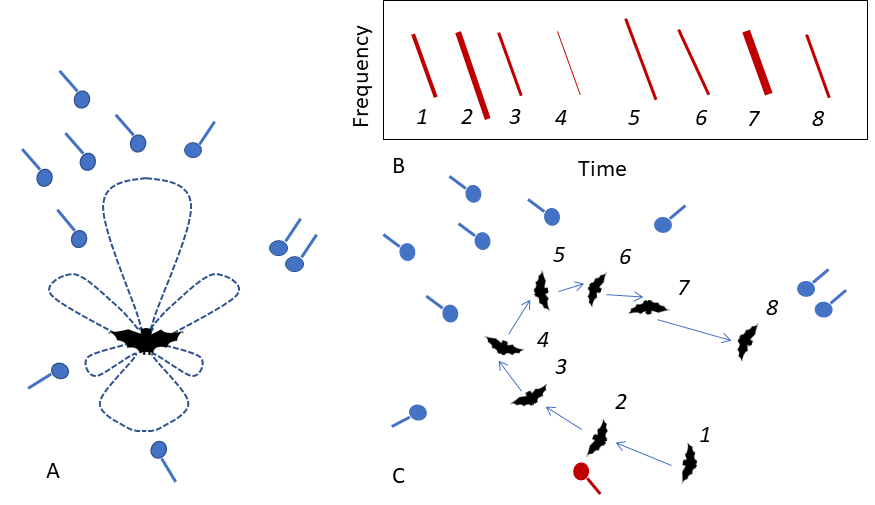
\includegraphics[width=1\linewidth]{original_papers/ushichka-figures/beamshape_cleaned} \caption{The benefits of multi-mic arrays for the study of echolocation and voice recognition (microphone: blue circle with line attached) A) Biosonar beam-shape can be estimated from microphones spread around the animals B,C) As the bat moves through the volume (C 1-8), the amplitude and spectral properties of the call received by the focal microphone (red) changes, as seen on the spectrogram (B). Having multiple microphones provides a multi-view picture of a call from many directions, allowing a better assessment of intra-individual call variation required for robust voice recognition}\label{fig:beamshape}
\end{figure}

The echolocation strategies in use may also inform why certain types of apparently stereotypical flight paths are seen within the recording volume. It was observed that bats sometimes tend to fly a circular loop close to the edges of the recording volume before leaving the cave or heading back into the roosting site (Figure \ref{fig:loopingsch}). This `looping' flight behaviour was observed in the evening flight activity as bats began to accumulate in the recording volume, but also when bats returned alone in the morning. Bats are known to show stereotypic flight behaviours in the lab and in the wild \citep{barchi2013spatial, mohres1949versuche}, and this may perhaps be due to their limited attention or spatial memory. However, in a cave setting, where there are no obvious obstacles, what drives the formation of these looping behaviours? Do the loops form a type of stereotypic trajectory that allows the bat to limit its attention only along that route? Why do bats not take the shortest path and fly from the exit straight into roosting site? Initial observations of group flights suggested that even when multiple bats were flying together, not all parts of the recording volume were being `used' by the bats. Some regions of the recording volume (regions close to walls) seemed to have a higher density of bats. Is this wall-clinging behaviour a behavioural adaptation to maintain a high received level of wall-echoes (in the presence of non-target sounds)? The wall-clinging behaviour is somewhat reminiscent of structure-following behaviour seen in the field with horsehoe bats, that follow hedgerows instead of taking shortcuts over open fields. Horseshoe bats however, are likely to follow structures due to the limited sensing range from their high-frequency echolocation - why would myotids also adopt this behaviour? Another interesting parameter to estimate is the dynamics of the loop's chirality (clockwise/counter-clockwise) with group size. Alignment is a standard measure of how similar animals are in their direction of movement. When there are multiple animals in the recording volume, a measure of the alignment over time and group size might reveal whether the looping behaviour is an individually driven behaviour or is modulated by the flight directions of group members.

\begin{figure}
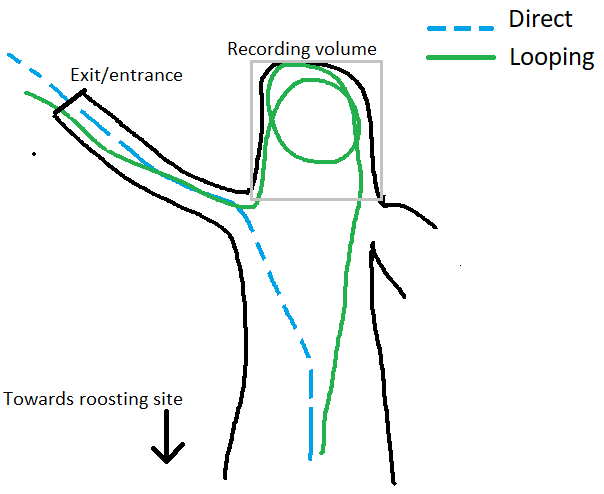
\includegraphics[width=1\linewidth]{original_papers/ushichka-figures/looping} \caption{Schematic showing a top view of the direct and looped flight paths as seen from above. The direct (broken blue line) and indirect (continuous green line) paths are flown in both directions (exit/entrance-cave interior, cave interior-exit/entrance). The grey quadrilateral outlines the recording volume.}\label{fig:loopingsch}
\end{figure}

\hypertarget{voice-recognition-for-short-term-and-long-term-behavioural-tracking}{%
\subsection{Voice recognition for short-term and long-term behavioural tracking}\label{voice-recognition-for-short-term-and-long-term-behavioural-tracking}}

Many vocalising vertebrates across the animal kingdom have individually identifiable vocalisations, or voices \citep{carlson2020individual}. The voice of each animal is a temporally stable cue, unlike experimental markings which may be lost over time. Despite the known stability of voice, one of the main challenges with developing a stable voice identifier is the variation in the vocalisation itself. Bird call repertoires can change over time, and complicate identification \citep{stowell2019automatic}. Approaches to date rely on machine-learning and statistical models, which require a training dataset of example vocalisations to `learn' the patterns in the data. Variation caused by sound directionality, distance and ambient noise may require larger training datasets, which are often hard to obtain \citep{stowell2019automatic}. Unlike many types of animal vocalisations (eg. bird song, mammal vocalisations), the spectro-temporal structure of bat echolocation calls are stereotypical and likely to remain stable because they serve a single sensory purpose -- to detect objects. The dedicated sensory functionality of echolocation calls, and the general absence of background ultrasonic noise in the wild makes bat calls a convenient system to develop voice identification workflows.

Bat echolocation calls can be assigned to individuals by their acoustic features, though this has typically been done in small lab populations. Previous work \citep{masters1995sonar, yovel2009voice} solved the `closed-set' problem where all animal identities are known. \emph{Ushichka} provides a large dataset over multiple nights and animals that fly by {[}also see Figure \ref{fig:beamshape} B,C{]}. In contrast to the `closed-set' problems solved in the past, \emph{Ushichka} could be used to generate methods to solve the `open-set' voice recognition task. Open-set classification problems deal with models that uniquely identify individuals that they have been trained on, but also those they have \emph{not} been explicitly trained on. Even though the identities of bats echolocating in the recordings are unknown, it may be possible to exploit the behavioural patterns of the animals to approximate identity. Bats always return alone in the morning, and these recordings contain multiple echolocation calls from one individual as it enters the recording volume and heads away to the roosting site. In addition, it is known that a stable population of resident female \emph{M. myotis/blythii} roost in the cave system over the entire summer period. Using these two facts, if successful, a voice recognition model should at least show certain patterns: 1) correctly assign identity to an independent subset of calls it was not trained on (validation data) from morning recordings 2) identify at least some individuals consistently across multiple morning returns, and in the best case 3) be able to pick up the individuals as they begin their activity in the recording volume around sunset. Of course, even if a trained model satisfies the three criteria above, it does not directly follow that the detections in scenarios 2) and 3) are not false positives. It may be necessary to systematically collect a larger sample of echolocation calls from hand-released individuals. The state of signal-processing and machine learning know-how in the field of human voice recognition is relatively mature at this point, with the use of speaker-specific Gaussian Mixture Models compared to Universal Background Models trained against multiple individuals \citep{Hennebert2009}. \emph{Ushichka} may provide a test-dataset to examine how well the latest voice recognition approaches perform for echolocation calls.

While seemingly challenging, if a validated voice recognition model is indeed developed successfully, it will allow revolutionary markerless short-term and long-term tracking of individual behaviours. Short-term behaviours such as flight and echolocation decisions over the course of a few seconds can provide insights into individual sensorimotor strategies and the tracking of social interactions. Long-term decisions such as the change of evening cave exit-time and morning return times can reveal the changing physiological status of the resident females as their pups mature. Voice based individual recognition brings the same advantages gained by tracking mammals with unique visible markings (eg. zebras, tigers) \citep{lahiri11_biometric, hiby2009tiger}, allowing unobtrusive observations over multiple time-points and scales.

\hypertarget{supplementary-code-and-website}{%
\section{Supplementary code and website}\label{supplementary-code-and-website}}

The \texttt{fieldrecorder\_trigger} module used to trigger automatic recording is uploaded at the following repository: \url{https://github.com/thejasvibr/fieldrecorder}. Those interested in viewing more snippets of the the \emph{Ushichka} dataset and the progress of research related to it, may wish to visit \url{https://thejasvibr.github.io/ushichka/}.

\hypertarget{field-work-permits}{%
\section{Field work permits}\label{field-work-permits}}

All field work at the Orlova Chuka cave was done with permission from the relevant authorities. \emph{Ushichka} is a purely observational dataset, no animals were handled or subjected to experimental treatments of any sort over the course of data collection.

\hypertarget{author-contributions-1}{%
\section{Author Contributions}\label{author-contributions-1}}

TB: conception, experiment design, field data collection. HRG: conception, experiment and recording-system design.

\hypertarget{acknowledgements-3}{%
\section{Acknowledgements}\label{acknowledgements-3}}

We would like to thank Antoniya Hubancheva, for her constant help and support in the collection of the \emph{Ushichka} dataset (also for christening the dataset with its Bulgarian name) and the Tabachka field crew of 2018. The electronics (Markus Abels, Hannes Sagunsky, Reinhard Biller) and Feinmechanik (Erich Koch, Felix Hartl, Klaus Pichler) teams were of invaluable help and support all through the process of experimental setup design and troubleshooting. We would like to thank Pranav Khandelwal for extensive help setting up the thermal camera calibration workflow and Hedrick Tyson for providing helpful feedback and estimating camera parameters. Fieldwork-wise, we are grateful to Joanna Furmankiewicz for supporting initial recordings at the Jaskinia Niedźwiedzia and Diane Theriault for providing advice on thermal cameras. Special thanks and acknowledgement to the field assistance of Aditya Krishna and Neetash MR, without whom the data collection would not have been possible. T.B. was funded by a doctoral fellowship from the German Academic Exchange Service (DAAD) and the International Max Planck Research School for Organismal Biology. H.R.G. was funded by the Emmy Noether program of the German Research Foundation (DFG, GO 2091/2-1, GO 2091/2-2). We would like to thank the members of the Acoustic and Functional Ecology groups and the Max Planck Institute for Ornithology, Seewiesen for its support and infrastructure.

\hypertarget{ushichkasi}{%
\section{Supplementary Information}\label{ushichkasi}}

\hypertarget{ushichkaavmatch}{%
\subsection{Audio-video synchronisation and recording}\label{ushichkaavmatch}}

The audio-video recording was run by a callback function that repeatedly collected input audio and output signals to and from the soundcards in the form of data buffers (1024-2048 samples). The input buffer consisted of an \(M_{channels} \:X \:N_{samples}\) array, while the output buffer consisted of a \(3 \:X \:N_{samples}\) array. When a recording was triggered, all input buffer data were concatenated and saved into an audio file. When not triggered, the input buffer data was only used to measure audio level. The output buffer consisted of three channels. The first ouptut channel was a constantly output 25Hz square wave
sent to the thermal camera control box. This 25Hz square wave was the common signal which synchronised the frame capture of all three thermal cameras. The signals in the second and third channels were dependent on whether
a recording had been triggered or not. When a recording was not triggered, only zeros were sent to the second and third channel's data buffer. When a recording was triggered, the second channel's data consisted of a 20 kHz sine wave. The high-frequency sine wave triggered the simultaneous video recording in all three thermal cameras, and thus ensured frame-level synchronisation in the video files. On triggering, the third channel's data buffer was an attenuated version of the square wave signal being sent in channel 1. This attenuated square wave served as an inter-soundcard synchronisation signal. Despite the use of the inbuilt Word clock signal from the master sound card, the audio data received across devices was observed to be jittered by a varying number of samples in each recording\footnote{The jitter may have been introduced by impedance mismatch and internal reflections caused by the use of 50 Ohm BNC cables and T-splitters. Recent experiments with the same Fireface devices using 75 Ohm cables and an impedance matched signal splitter lead to constant synchronisation between multiple Fireface soundcards}. The audio data from within a single sound card was however verified to be sampled synchronously.

The automated audio-video recording was controlled by the \texttt{fieldrecorder\_trigger} module.

\hypertarget{automicpos}{%
\subsection{Automatic microphone position estimation}\label{automicpos}}

The Structure-From-Sound approach \citep{zhayida2016automatic} to automatically estimate microphone positions relies on a common sound being recorded simultaneously on multiple channels. The time-differences-of-arrival between channel pairs are used to estimate the positions of the microphones. \citet{zhayida2016automatic} use a continuous sound source such as a song or speech signal, while we chose to use discrete signal playbacks.

To automatically estimate the positions of the microphones placed all around the cave speaker playbacks were performed after each recording session as described in \citet{sfs_cotdoa}. Briefly, a speaker (Peerless XT25SC90-04) with an attached reusable heating pad was moved through the recording volume (Figure \ref{fig:sfsplayback}). The playback signals changed over the course of the field season. Playbacks from 19th June to 14th July 2018 used an upward swept hyperbolic sweep between 16-96 kHz, 8ms in duration played with a constant interval of one second. Playbacks from 21st June 2018 onwards used `multi-chirp' signals. Multi-chirp playbacks consisted of a packet of 9 sweeps made by a combination of three time-frequency structures (linear, hyperbolic, V-shaped) and three durations (6, 12, 24 ms). Each sweep occured at the end of a 200ms segment, and thus one packet of 9 sweeps was 1.8s long. Multiple packets were played with a 1.6s inter-packet silence between them. Playback signals were generated from the sound card in use (Fireface UC or Fireface 802), and amplified through a car audio amplifier (Basetech AP-2100). Playbacks were only conducted past 6:00 am to prevent disturbing the resident bat population (at this time of day, there are almost no bats flying in the recording volume). See \ref{recnights} for further details.

\citet{sfs_cotdoa} showed succesful position estimation using discrete playbacks with ground-truthed microphone positions from one night in the Ushichka dataset. The microphone position estimations reported by \citet{sfs_cotdoa} are within the range of \(\pm\) 4 cm of ground-truthed positions. This error-range may perhaps be sufficient for acoustic tracking given that the bat-microphone distances are much larger (in the order of 0.5-5m).

Additional audible speaker playbacks were also performed from a small portable speaker. However, this data is yet to be analysed.

\begin{figure}
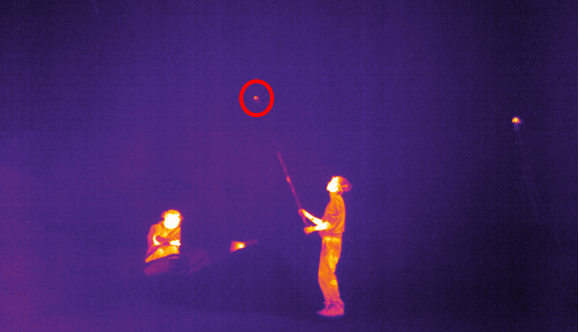
\includegraphics[width=8.04in]{original_papers/ushichka-figures/speaker_w_heatpad} \caption{\label{fig:sfsplayback} An image taken from the synchronised video recording captured during playbacks conducted for automatic mic position estimation. The red circle highlights the position of the speaker.The speaker was attached to the end of a rod. The rod was moved in such a manner that playbacks were recorded from all over the recording volume. The speaker was made visible on the thermal video by a warming pad attached behind it, and thus also allows 3D video tracking of its position.}\label{fig:sfsplayback}
\end{figure}

\hypertarget{microphone-frequency-response-and-directionality-calibration}{%
\subsection{Microphone frequency response and directionality calibration}\label{microphone-frequency-response-and-directionality-calibration}}

Inital mic frequency response and directionality measurements were done on 11th January 2019 for a subset of 15 microphones (4 SANKEN CO-100 and 11 SMP Knowles 0410's). The microphone was placed at a distance of 1.11 m from the speaker. Both microphone and speaker were aligned and placed on tripod stands away from the ground to avoid ground-reflections. The playback signal was a combination of pure tones (10-95 kHz, in 1 kHz steps, Tukey-windowed) and linear sweeps (10 ms, 15-95 kHz, Tukey-windowed). The linear sweep was repeated five times. The same playback was recorded at a variety of azimuth and elevation angles. Only one side (left/right or up/down) was recorded as symmetry was assumed across the azimuth and elevation.

Each microphone was attached to a L-shaped holder that was centred around a rotation point. The tip of the SANKEN CO-100's were set to be over the rotation point. The Knowles SPU 0410 microphones were attached to a cardboard sheet to mimic the effect of the cave wall. This allowed replication of the frequency and directionality response the microphones would have had in the cave. The cardboard sheet was aligned to coincide with the rotation point.

For reference, a calibration microphone (GRAS 40BF, GRAS Sound and Vibration, Denmark) attached to a pre-amplifier (GRAS Type 26AC) and amplifier (GRAS Type 12HF) was placed in the same location as the microphones under calibration and the calibration playbacks were recorded.

\hypertarget{ushichkacamcalib}{%
\subsection{Camera calibration}\label{ushichkacamcalib}}

The three thermal cameras were calibrated for their extrinsic (position and orientation) and intrinsic (focal length and distortion) parameters using the `wand' procedure and `easyWand' package described in \citet{Theriault2014}. Two halogen lamps (G4, 20W, 12V)
were attached to the ends of a wooden stick (lamp-to-lamp distance of 59cm) and connected in parallel to a 12V DC car battery, forming the `thermal wand'. The small size of the hot halogen lamps meant that the lamps appeared as points on the video and were easy to localise in the video data. The wand was moved systematically within the recording volume to cover all parts where bats flew.

\begin{figure}
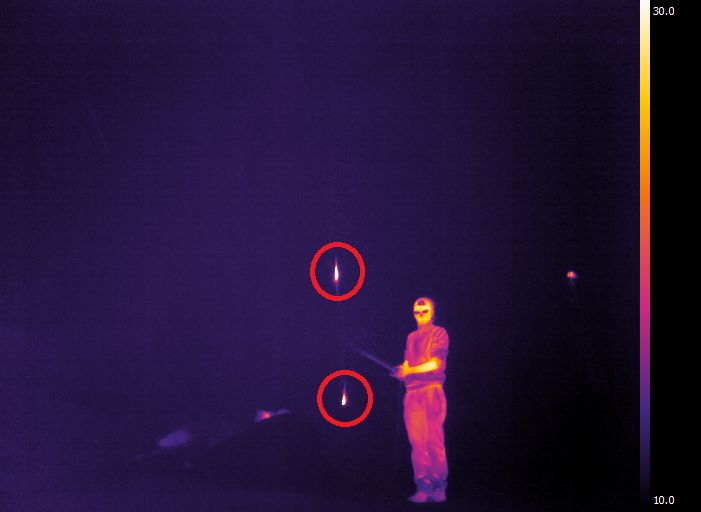
\includegraphics[width=9.74in]{original_papers/ushichka-figures/wand_marked_} \caption{Image showing the thermal wand used as the common calibration object. The two incandescent lights forming either end of the wand are encircled in red.}\label{fig:wandimg}
\end{figure}

Wand points were digitised using the DLTdv package \citep{dltdv} and preliminary Wand scores from calibrations done using the easyWand package\cite{Theriault2014} gave a `wand score' of \(< 1\), indicating a relatively good calibration. The Wand score indicates the variation in estimated distance between the two wand points across the calibrated volume, where a low score indicates a good calibration. In addition, gravity calibration was also performed by throwing a reusable click-activated heating pad.

\hypertarget{additional-video-recordings-of-relevance-in-ushichka}{%
\subsection{\texorpdfstring{Additional video recordings of relevance in \emph{Ushichka}}{Additional video recordings of relevance in Ushichka}}\label{additional-video-recordings-of-relevance-in-ushichka}}

Aside from bat flight and wand video recordings, a series of other video recordings were also performed. These video recordings serve to provide at least two functionalities. The first function is to align audio and video tracking data into a common co-ordinate system. The second function is that the video recordings provide `background points' (sensu \citet{Theriault2014}) to assist camera parameter estimations.

\begin{enumerate}
\def\labelenumi{\arabic{enumi}.}
\item
  Mic positions : For every recording night, the positions of microphones were `pointed' at with the thermal wand. These recordings are particularly useful to align the acoustic and video tracking data into a common coordinate system.
\item
  Speaker playback recordings: The speaker playbacks for mic position estimation described in \ref{automicpos} were recorded simultaneously with audio and video (See Figure \ref{fig:sfsplayback}). While these recordings could be used to align audio and video, they will be less accurate as the heating pad is placed at a slight distance from the speaker. The speaker playback recordings are thus better used to add `background points' to improve camera parameter estimations.
\end{enumerate}

\hypertarget{recnights}{%
\subsection{Recording nights in the recording volume}\label{recnights}}

\begin{longtable}[]{@{}llll@{}}
\caption{\label{tab:nightandplayback} Table showing the date of recording session and type of playback. The multi-chirp sweeps consisted of linear, hyperbolic and V-shaped sweeps each with short,medium and long durations of 6,12,24ms length respectively. Sessions with manually triggered recordings were triggered by an experimenter listening for bat calls on a bat detector while watching the thermal camera video feed. Automaticallyally triggered recordings were set to start when the RMS of an incoming audio buffer crossed a threshold value.}\tabularnewline
\toprule
Session Date & Playback signal type & Duration (ms) & Recordings triggered\tabularnewline
\midrule
\endfirsthead
\toprule
Session Date & Playback signal type & Duration (ms) & Recordings triggered\tabularnewline
\midrule
\endhead
2018-06-19 & Hyperbolic & 8 & Manually\tabularnewline
2018-06-21 & Hyperbolic & 8 & Manually\tabularnewline
2018-06-22 & Hyperbolic & 8 & Automatically\tabularnewline
2018-07-14 & Hyperbolic & 8 & Automatically\tabularnewline
2018-07-21 & Multi-chirp & 6,12,24 & Automatically\tabularnewline
2018-07-25 & Multi-chirp & 6,12,24 & Automatically\tabularnewline
2018-07-28 & Multi-chirp & 6,12,24 & Automatically\tabularnewline
2018-08-14 & Multi-chirp & 6,12,24 & Automatically\tabularnewline
2018-07-28 & Multi-chirp & 6,12,24 & Automatically\tabularnewline
2018-08-02 & Multi-chirp & 6,12,24 & Automatically\tabularnewline
2018-08-14 & Multi-chirp & 6,12,24 & Automatically\tabularnewline
2018-08-17 & Multi-chirp & 6,12,24 & Automatically\tabularnewline
2018-08-18 & Multi-chirp & 6,12,24 & Automatically\tabularnewline
2018-08-19 & Multi-chirp & 6,12,24 & Automatically\tabularnewline
\bottomrule
\end{longtable}

\hypertarget{sfscotdoa}{%
\chapter{Robust Self-Calibration of Constant Offset Time-Difference-of-Arrival}\label{sfscotdoa}}

\chaptermark{Microphone self-calibration}

This chapter was published as a peer-reviewed paper in the conference proceedings of the International Conference on Acoustics, Speech, and Signal Processing:

\emph{Batstone, K., Flood, G., Beleyur, T., Larsson, V., Goerlitz, H. R., Oskarsson, M., \& Åström, K. (2019, May). Robust self-calibration of constant offset time-difference-of-arrival. In ICASSP 2019-2019 IEEE International Conference on Acoustics, Speech and Signal Processing (ICASSP) (pp.~4410-4414). IEEE.}

\newpage

\hypertarget{sfsabstract}{%
\section*{Abstract}\label{sfsabstract}}
\addcontentsline{toc}{section}{Abstract}

In this paper we study the problem of estimating receiver and sender positions from time-difference-of-arrival measurements, assuming an unknown constant time-difference-of-arrival offset. This problem is relevant for example for repetitive sound events. In this paper it is shown that there are three minimal cases to the problem. One of these (the five receiver, five sender problem) is of particular importance. A fast solver (with run-time under \(4~ \mu s\)) is given. We show how this solver can be used in robust estimation algorithms, based on RANSAC, for obtaining an initial estimate followed by local optimization using a robust error norm. The system is verified on both real and synthetic data.

\newpage

\hypertarget{introduction-3}{%
\section{Introduction}\label{introduction-3}}

The problem of estimating receiver-sender node positions from measured arrival times of radio or sound signals is a key issue in different applications such as microphone array calibration, radio antenna array calibration, mapping and positioning. This field is well researched but in this paper we will focus on the anchor-free sensor network calibration both in terms of time-of-arrival measurements (TOA) and time-difference-of-arrival measurements (TDOA).
For time-of-arrival the planar case of three receivers and three senders (3R/3S) was solved in \cite{stewenius-phd-2005}.
For the full 3D case the over-determined problem (10R/4S) was studied in \cite{pollefeys-nister-icassp-08}, where a solver for this non-minimal case was provided. There are actually three minimal cases for the 3D case, namely (4R/6S), (5R/5S) and (6R/5S). A practical solver was presented in
\cite{kuang-burgess-etal-icassp-13}. There are in general \(38\), \(42\) and \(38\) solutions respectively for the three different set ups.
Faster solvers for these minimal cases were provided in \cite{larsson2017polynomial}.

In this paper we study the constant offset TDOA self-calibration problem. It is a problem that naturally arises e.g.~when signals are emitted with a known period. As an estimation problem it lies between TOA and full TDOA. In the paper we study the minimal (5R/5S) problem and provide a fast (few \(\mu s\)) solver.
Robust parameter estimation often use the hypothesize and test paradigm, e.g.~using random sampling consensus, \cite{fischler-bolles-ca-81} or one of its many variants (\cite{chum2003locally,raguram2013usac,korman2018latent}). In these frameworks minimal solvers are important building blocks for generating model hypotheses, and we show in the paper how a minimal solver can be used for robust parameter estimation of sender positions, receiver positions and unknown offset. The system is capable of handling missing data, outliers and noise. The algorithms are tested on synthetic data as well as real data, in an office environment and in a cave.The methods are straightforward to generalize for degenerate configurations which arise if senders or receivers are restricted to a plane or to a line.

\hypertarget{time-difference-of-arrival-self-calibration}{%
\section{Time-difference-of-arrival self calibration}\label{time-difference-of-arrival-self-calibration}}

The problem we are considering involves \(m\) receiver positions \(\mathbf{r}_i \in \mathbb R^3\), \(i = 1, \dots, m\) and \(n\) sender positions \(\mathbf{s}_j \in \mathbb R^3\), \$ j = 1, \dots, n\$. This could for example represent the microphone positions and locations of sound emissions, respectively. Assume that the arrival time of a sound \(j\) to receiver \(i\) is \(t_{ij}\) and that the time that sound \(j\) is emitted is \(T_j\).
Multiplying the travel time \(t_{ij} - T_j\) with the speed \(v\) of the signal we obtain the distance between senders and receiver,

\begin{equation}
v (t_{ij}-T_j)   = {\norm{\mathbf{r}_i - \mathbf{s}_j}}_2 ,
\label{eq:tdoa}
\end{equation}
where \({\norm{.}}_2\) is the \ltwo-norm. The speed \(v\) is throughout the paper assumed to be known and constant.

In many settings the times of emissions \(T_j\) are unknown, but regular, \eg
\begin{equation}
T_j = k_1 j + k_0, 
\label{eq:regular}
\end{equation}
where the interval \(k_1\) is known. Inserting \eqref{eq:regular} into \eqref{eq:tdoa} we
obtain
\begin{equation}
v (t_{ij}-k_1 j - k_0)   = {\norm{\mathbf{r}_i - \mathbf{s}_j}}_2 . 
\end{equation}
Assuming an erroneous (but regular) emission time
\(\tilde{T}_j = k_1 j + \tilde{k}_0\) and
introducing (the measured) \(z_{ij} = v (t_{ij}-\tilde{T}_j)\) and (the unknown) \(o = v (k_0-\tilde{k}_0)\) yields the following expression
\begin{equation}
 z_{ij}   = {\norm{\mathbf{r}_i - \mathbf{s}_j}}_2 + o. 
\end{equation}
Note that this is a simplified variant of the general time-difference-of-arrival problem (see \eg  \cite{kuang2013stratified}), which allows for a different offset \(o\) for every \(j\),
\begin{equation}
 z_{ij}   = {\norm{\mathbf{r}_i - \mathbf{s}_j}}_2 + o_j.
\end{equation}

\noindent 

\begin{problem1} \label{prob_misstoa}
({{Constant Offset Time-Difference-of-Arrival  Self-Calibration}}) Given measurements $\tilde{z}_{ij}$ 
\vspace{-5pt}
\begin{equation}
\tilde{z}_{ij} = {\norm{\mathbf{r}_i - \mathbf{s}_j}}_2 + o  + \epsilon_{ij}, 
\label{eq:distance}
\vspace{-5pt}
\end{equation}
for a subset $W \subset I$ of all the receiver-sender index pairs $I = \{ (i,j) | i = 1, \ldots m, j = 1, \ldots, n \}$ determine receiver positions $\mathbf{r}_i$, $ i = 1, \dots, m$ and sender positions $\mathbf{s}_j$,  $j = 1, \dots, n$ and offset $o$. 
Here the errors $\epsilon_{ij}$ are assumed to be either 
{\bf inliers}, in which case the errors are small ($\epsilon_{ij} \in N(0,\sigma)$) or {\bf outliers}, in which case the measurements are way off. 
\end{problem1}

Here we will use the set \(\Win\) for the indices \((i,j)\) corresponding to the inlier measurements and \(\Wout\) for the indices corresponding to the outlier set.
\vspace{-5pt}

\section{Local optimization and the low~rank~relaxation}
\label{sec:rank}
\vspace{-5pt}

If an initial estimate of the parameters \(\theta_1 = \{ R, S, o \}\) is given and if the set of inliers is known, then refinement of the estimate can be found by optimization methods, \eg Levenberg-Marquardt (LM) (\cite{levenberg1944method,marquardt1963algorithm}),
\begin{equation}
\min_{\theta_1} f(\theta_1) = \sum_{(i,j) \in \Win} (z_{ij} - ( {\norm{\mathbf{r}_i - \mathbf{s}_j}}_2 +o) )^2 .
\end{equation}

There is an interesting relaxation to the problem, that exploits the fact that the matrix with elements \((z_{ij}-o)^2\) is rank \(5\), (\cite{pollefeys-nister-icassp-08}). Further simplifications use the double compaction method (\cite{kuang2013stratified}). The double compaction matrix \(M\) is defined as the matrix with elements
\begin{equation}
M_{ij}=(z_{ij}-o)^2 -a_i-b_j,
\label{eq:dc}
\end{equation}
and it can be shown to have rank \(3\), i.e.~\(M = U^T V\), where \(U\) is of size \(3 \times m\) and \(V\) is of size \(3 \times n\).
The relaxed problem involves a set of parameters
\(\theta_2 = \{ U, V, b, a, o \}\). Here the constraints can be written as
\begin{equation}
z_{ij} =  \sqrt{u_i^T v_j + a_i + b_j} + o ,
\end{equation}
where \(u_i\) denotes column \(i\) of \(U\) and \(v_j\) denotes column \(j\) of \(V\).
Refinement of parameters can be done by performing local optimization on
\begin{equation}
\min_{\theta_2} f(\theta_2) = \sum_{(i,j) \in \Win} \left ( z_{ij} - ( \sqrt{u_i^T v_j + a_i + b_j} + o ) \right )^2 .
\label{eq:relaxed}
\end{equation}

\vspace{-5pt}
\section{Minimal problems and solvers}
\label{sec:minimal}
\vspace{-5pt}

By counting equations and unknowns, one finds that there are three minimal problems. The first two are the symmetric case when \(m=4, n=7\) or \(m=7, n=4\). This case is not addressed in this paper, but we believe it to be difficult to solve. The other case is \(m=n= 5\). Here, we first present a solver for the constant offset and then discuss how to solve for sender and receiver positions.

Given a \(5 \times 5\) matrix, \(Z\), with time-difference-of-arrival measurements \(z_{ij}\), the rank \(3\) constraint on the double compaction matrix in \eqref{eq:dc}
can be written as
\begin{equation}
f(o) = \det ( C^T (Z-o)^{\circ 2} C )  = 0, 
\end{equation}
where
\begin{equation}
C = \begin{pmatrix}
-1 & -1 & -1 & -1\\
1 & 0 & 0 & 0\\
0  & 1 & 0 & 0\\
0 & 0 & 1 & 0 \\
0 & 0 & 0 & 1 
\end{pmatrix} 
\end{equation}
and \(^{\circ 2}\) denotes element-wise squaring (Hadamard power).
Although the elements of \((Z-o)^{\circ 2}\) are of degree 2 in \(o\), the quadratic terms cancel out after multiplication with \(C^T\) and \(C\). Thus the elements of \(C^T (Z-o)^{\circ 2} C\) are linear in \(o\).
Since the determinant is linear in each column, the determinant \(f(o)\) is a polynomial of degree four in the offset \(o\). This can be summarized as

\begin{theorem}
Given time-difference-of-arrival measurements from five receivers to five senders, there are four possible offsets $o$, given as the roots to the fourth degree polynomial $f(o)$, counting complex roots and multiplicity of roots. 
\end{theorem}

For each solution \(o\) it is possible to generate a solution \(\theta_2\) to the relaxed problem,
according to

\begin{equation*}
\! b \! = \! \begin{pmatrix} (z_{11} \! - \! o)^2  \! \!  &  \! \!  (z_{12}-o)^2  \! \!  &  \! \!  (z_{13}-o)^2 \! \!  &  \! \!   (z_{14}-o)^2 \! \!  &  \! \!   (z_{15}-o)^2 \end{pmatrix} \! ,
\end{equation*}
\begin{equation}
a =  \begin{pmatrix} 0 \\ (z_{21}-o)^2 -(z_{11}-o)^2\\ (z_{31}-o)^2 -(z_{11}-o)^2 \\ (z_{41}-o)^2 -(z_{11}-o)^2 \\ (z_{51}-o)^2 -(z_{11}-o)^2 \end{pmatrix},
\end{equation}
\begin{equation}
U =  \begin{pmatrix} 0 & u_2 & u_3 & u_4 & u_5\end{pmatrix}, 
\end{equation}
\begin{equation}
V =  \begin{pmatrix}0 & v_2 & v_3 & v_4 & v_5\end{pmatrix} ,
\end{equation}
where \(\begin{pmatrix}u_2 & u_3 & u_4 & u_5\end{pmatrix}^T \begin{pmatrix} v_2 & v_3 & v_4 & v_5\end{pmatrix}\) is any rank \(3\) factorization of the matrix \(C^T (Z-o)^{\circ 2} C\).

From a solution \(\theta_2\) to the relaxed problem it is possible to upgrade to a solution \(\theta_1\) to the original problem. This involves solving a system of polynomial equations. The procedure was first described in \cite{kuang-burgess-etal-icassp-13}, where an algorithm for solving this was presented. Recently, a faster algorithm was presented in \cite{larsson2017polynomial}.

An efficient implementation for calculating the four solutions of the offset \(o\) given the measurements \(z\) takes \(4~ \mu s\) for a C++-implementation. Generating the solution \(\theta_2\) to the relaxed problem adds a few \(\mu s\). However, calculating a solution \(\theta_1\) to the original problem takes another \(22 ~ms\). Thus, it is advantageous to estimate the parameters of the relaxed problem and postpone the upgrade from \(\theta_2\) to \(\theta_1\) as a final step, see Table \ref{Tabletime}.

\begin{table}
\caption{Execution times for $5 \times 5$ minimal solvers steps. Notice that the steps of calculating $o$ and the relaxed solution is significantly faster than upgrading to the full solution}
\centering
\vspace{4mm}
\begin{tabular}{@{}ccc@{}} \toprule
%& \multicolumn{5}{c}{CS (dB)} & \multicolumn{5}{c}{SSIM} \\ \cmidrule(r){2-11}
Implementation & Matlab  & C++ \\
\midrule 
Calculation of $o$ & $38 \, \mu s$ & $3.7 \, \mu s$ \\
Calculation of $\theta_2 = \{ U,V,a,b,o \}$ & $100 \, \mu s$ & N/A \\
Calculation of $\theta_1 = \{ R,S,o \}$ & $600 \, ms$ & $22 \, ms$ \\
\bottomrule
\end{tabular}
\label{Tabletime}
\end{table}

\vspace{-5pt}

\section{Using RANSAC for five rows}
\label{sec:ransac}
\vspace{-5pt}

We propose the use of the fast minimal solver in an hypothesize and test framework to obtain (i) a initial estimate on the offset \(o\) and (ii) an initial inlier set. The steps are described in Algorithm\textasciitilde{}\ref{a_offset}

\begin{algorithm}
\caption{Offset RANSAC}\label{a_offset}
\begin{algorithmic}[1]
\State Randomly select $5$ rows and columns. Find the four solutions on $o$ given the time-difference-of-arrival measurements. 
\State For each solution $o$, calculate the relaxed solution $\theta_2 = \{ U,V,a,b,o \}$.
\State For selected rows and for each remaining column, check for inliers according to the residuals in \eqref{eq:relaxed}.
\end{algorithmic}
\end{algorithm}

\vspace{-5pt}
\section{Robust estimation of parameters}
\label{sec:ransac}
\vspace{-5pt}

We use these minimal solvers with RANSAC as described in the previous section to find one or several initial estimates of the parameters \(\theta_2\) for a subset of five receivers and \(k\) senders. The solution is extended to additional rows and/or columns using robust techniques as described in \cite{batstone2016robust}. During this process it is useful to keep the errors down by occasionally refining the solutions using local optimization. This has shown to reduce failures, see e.g.~(\cite{engels-stewenius-etal-06,klein2007parallel}).
In the proposed estimation algorithm we postpone the upgrade from \(\theta_2\) to \(\theta_1\) until we have found a good solution involving a large portion of the receiver and sender positions.
\vspace{-5pt}

\section{Experimental Validation}
\label{sec:exp}
\vspace{-5pt}
\subsection{Minimal Solver}
\vspace{-5pt}

To test the numerical accuracy and robustness of our minimal solver we conducted an experiment using simulated data without noise. We generated a large number of instance problems (10,000) with known offsets. We then ran our solvers and compared the returned solutions with the ground truth solution. For each instance problem we recorded the distance to the closest solution. In Figure \ref{fig:f_hist} the resulting histogram of the logarithm of the absolute errors are shown. As can be seen, both implementations get close to machine precision.

\begin{figure}
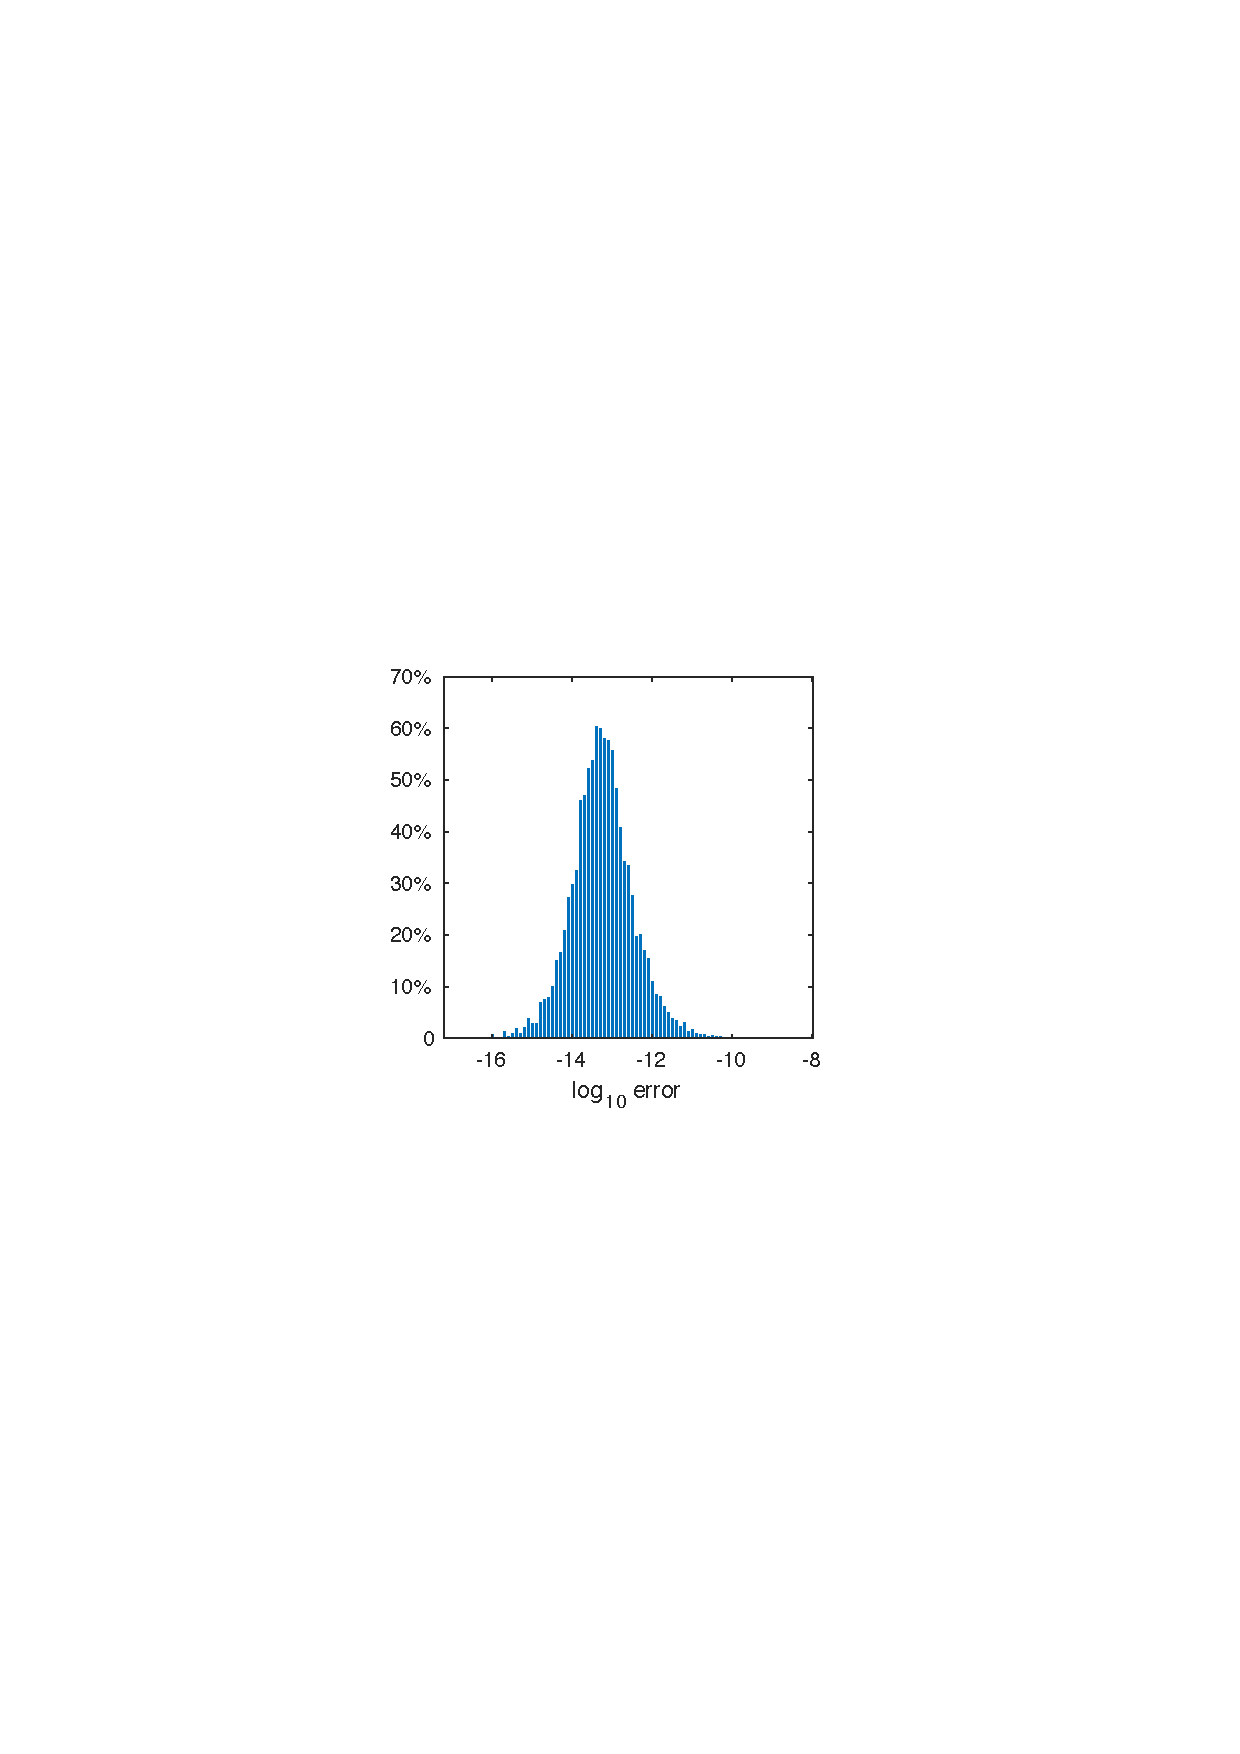
\includegraphics[width=0.4\textwidth]{original_papers/icassp_2018/figs/hist_matlabsolver.pdf}
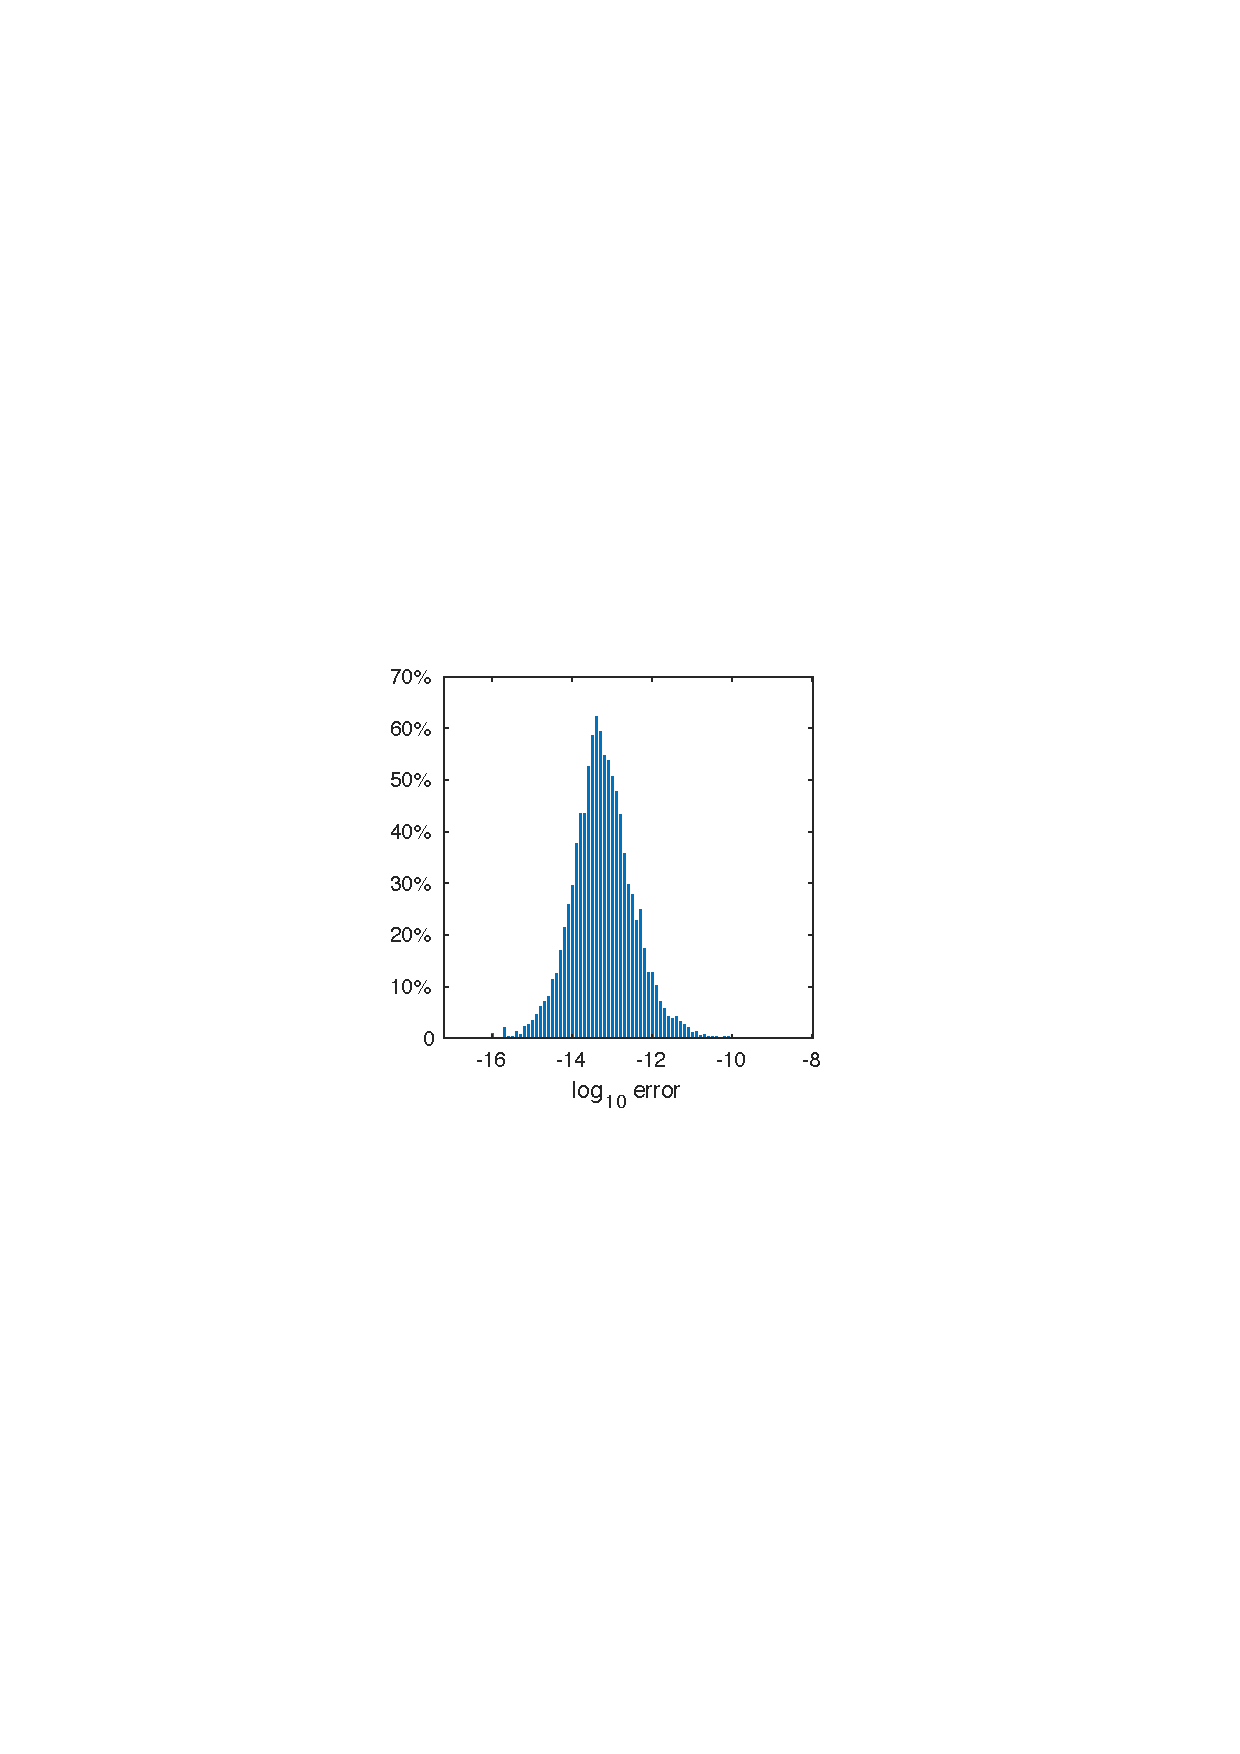
\includegraphics[width=0.4\textwidth]{original_papers/icassp_2018/figs/hist_mexsolver.pdf}
\caption{Left shows the histogram of the logarithm of the absolute errors, for the Matlab implementation of our minimal solver. To the right the corresponding histogram for the C++ implementation.}
\label{fig:f_hist}
\end{figure}

\vspace{-5pt}
\subsection{Experimental Setup for Real Data}
\vspace{-5pt}

We have tested our system on (i) experiments made in an office environment and (ii) experiments made at the Orlova Chuka cave, Bulgaria.

For the office experiments, 12 microphones (8x t.bone MM-1, 4x Shure SV100) were positioned around a room (\(\sim 3 \times 5~m^2\)) and measured using a laser to obtain ground truth positions of the microphones with an error of \(\pm 2~ mm\). The space was cleared of most the furniture to create an open space to conduct the experiment in. The sound recordings were captured using a Roland UA-1610 Sound Capture audio interface and automatically amplified. The recordings were made using the open source software Audacity 2.3.0 with a sampling frequency of \(96~kHz\) on a laptop. A synthetically generated chirp was then played using a simple loudspeaker every half second for \(30~s\) while moving the speaker around in the room.

For the cave experiments, 12 microphones (4x Sanken CO-100K, 8x Knowles SPU0410) were positioned in a section of the cave, four microphones were placed on an inverted T array near one wall, while the other eight microphones were placed on the adjacent wall. The sound recordings were captured using pre-amplifiers (Quadmic, RME) and two synchronised Fireface 800 (RME) audio interfaces running at a sampling frequency of \(192 ~kHz\). Recording and playback were controlled via a custom written script based on the sound device library
(\cite{geier2015}) in Python 2.7.12 (\cite{van1995python}). Ultrasonic chirps (\(8~ms\), \(16-96~kHz\) upward hyperbolic sweep) were played every second via one of the audio interfaces, amplified (Basetech AP-2100) and presented through a Peerless XT25SC90-04 loudspeaker. The speaker was attached to a 3-m-long pole and slowly waved in the approximately \(5 \times 9 \times 3 ~m^3\) recording volume. Playbacks were done past 6:00 am to prevent disturbing the resident bat population.

\vspace{-5pt}
\subsection{Experimental Evaluation for Real Data}
\vspace{-5pt}

Once the office recordings were taken, an algorithm was used to find the chirps in the captured sound recordings and the algorithm then outputs the \(z_{ij}\) matrix. This can then be used in our RANSAC scheme, Algorithm\textasciitilde{}\ref{a_offset}. For this experiment we used the (5R/5S) minimal solver. A fixed number of iterations was used; 100 iterations for the initial selection of 5 receivers and senders, then the extension to more columns and rows was allowed until there was no better solution. The tolerance was set to \(T=0.01\) for the initial selection and extension of rows and column.

Once the initial values have been estimated, it underwent \(l^{2}\) optimization on the inlier set. The results of the estimated microphone positions after the optimization are shown in Figure \ref{f_454H}.

This produced an Euclidean distance error between each of the microphones calculated position and its ground truth position as (0.2016,0.0587,0.1444,0.1153,0.2017, 0.1326,0.1407, 0.1198,0.2041,0.2010,0.1908,0.2110) m.

For graphical purposes, a Procrustes fitting was used on the microphone positions to spread the total error over all 12 microphones. In the Procrustes fitting only rotation and translation were allowed.

For the cave experiment a similar scheme was devised and the results are shown in Figure \ref{f_bat}.

\begin{figure}
\begin{tabular}{c}
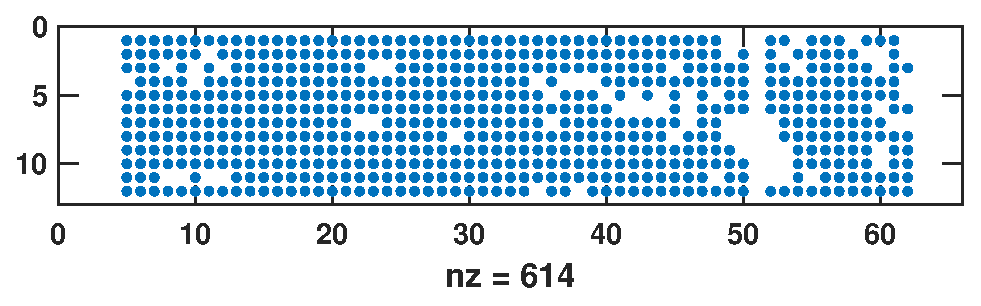
\includegraphics[width=0.8\textwidth]{original_papers/icassp_2018/figs/MH454_F_inl.eps} \\
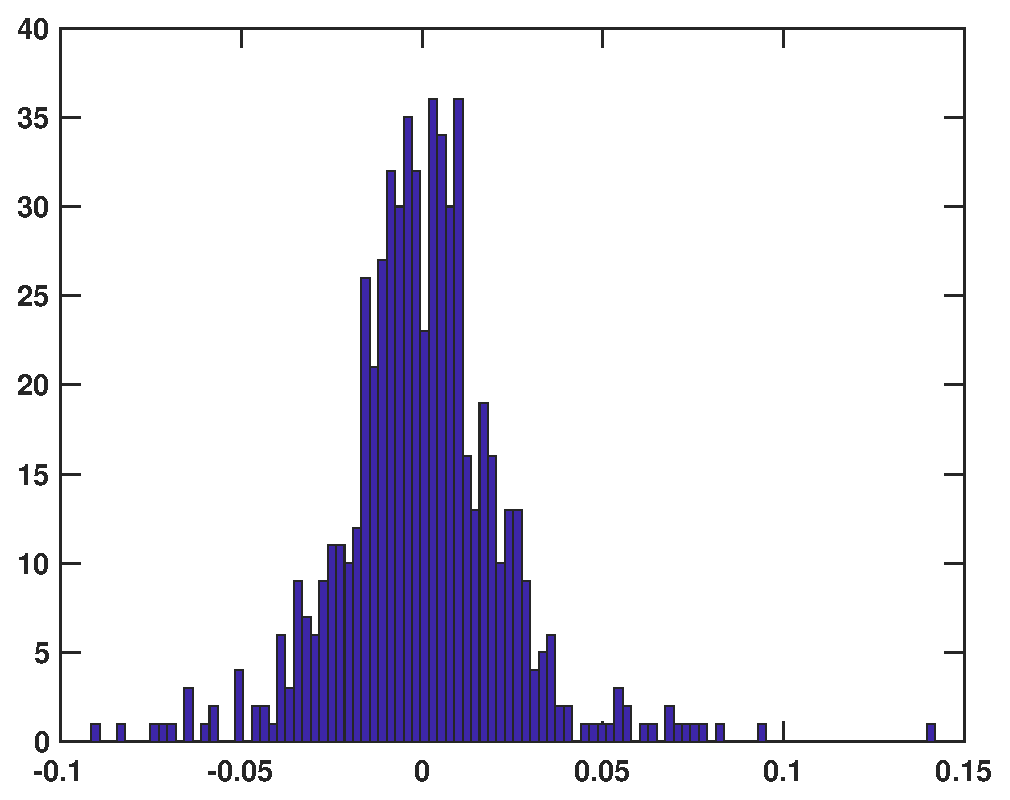
\includegraphics[width=0.4\textwidth]{original_papers/icassp_2018/figs/MH454_F_res.eps} 
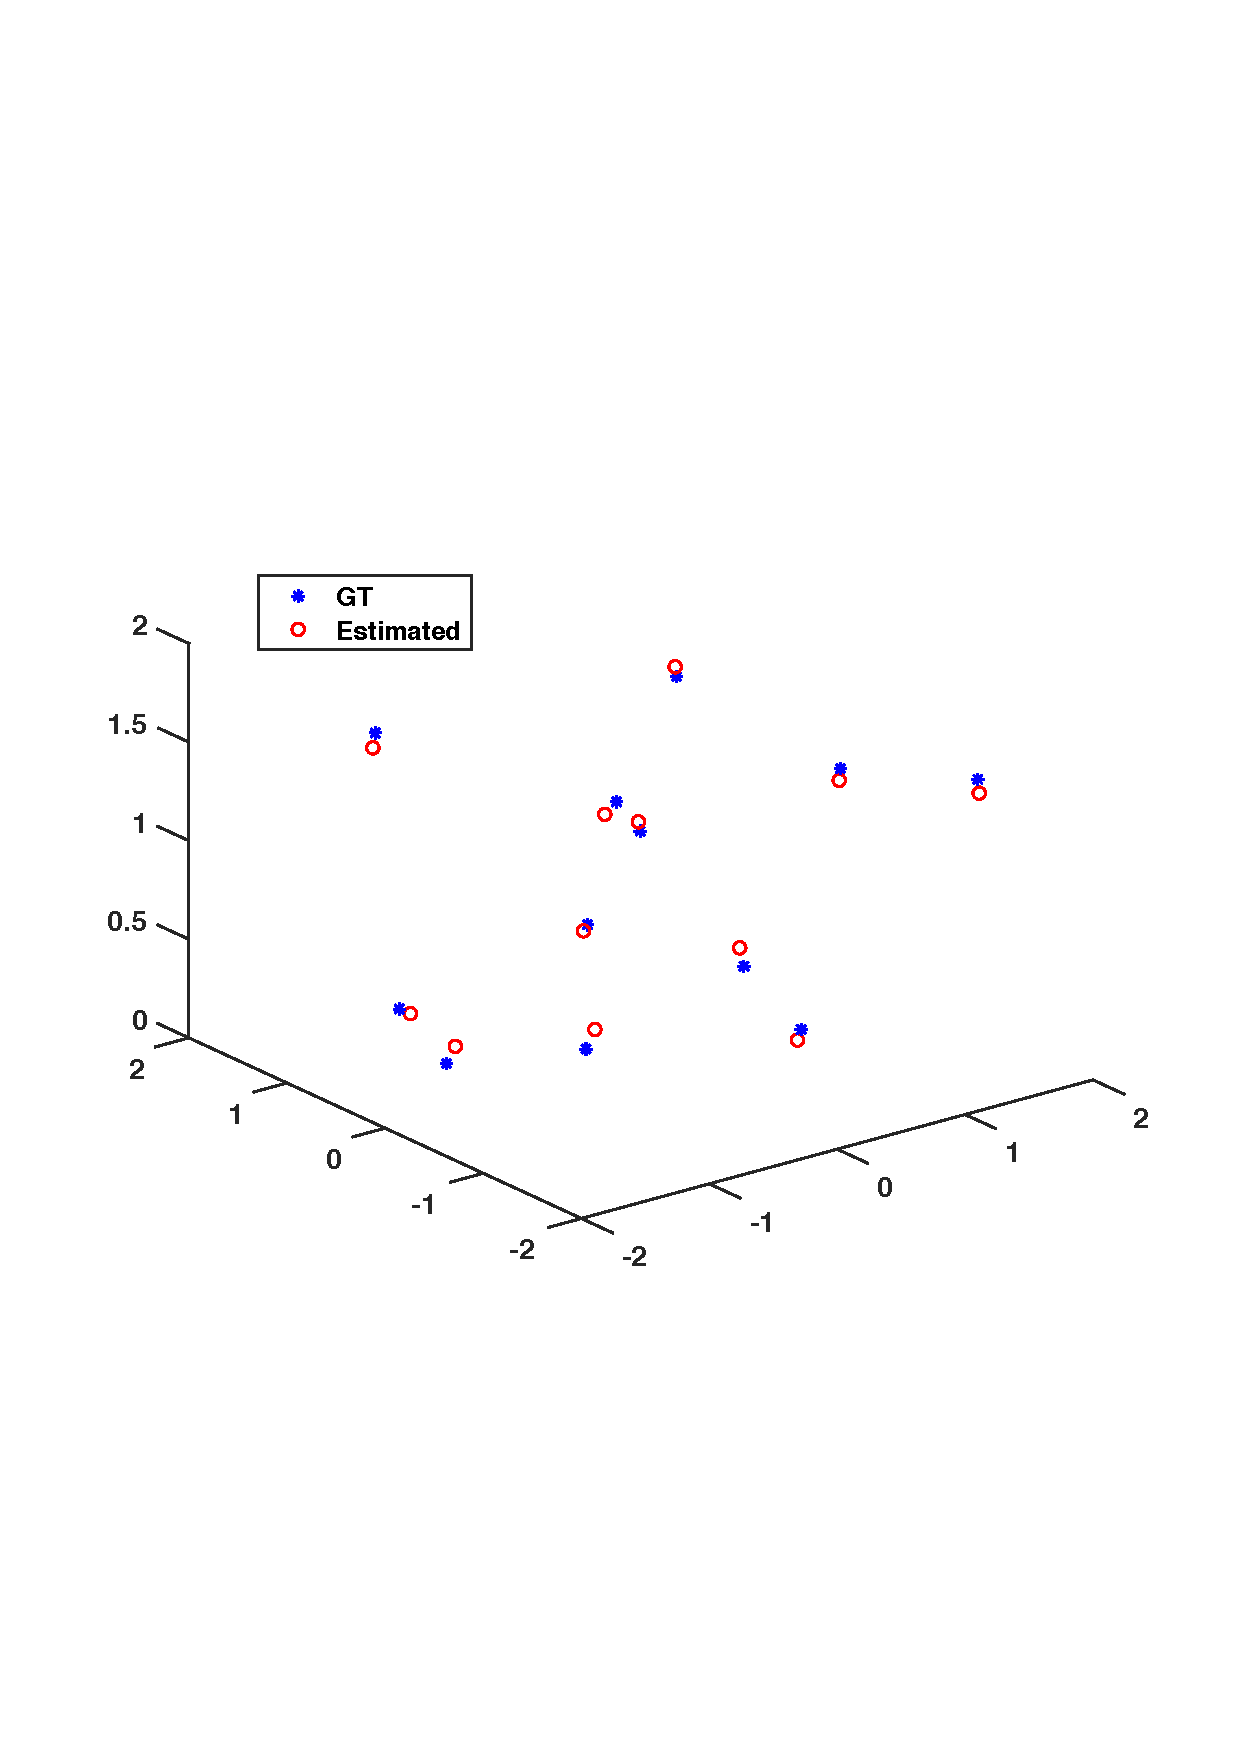
\includegraphics[width=0.4\textwidth]{original_papers/icassp_2018/figs/MH454_F_fig_new.pdf} 
\end{tabular}
\caption{For the office experiment the figure shows  detected inliers $\Win$ (top),  inlier residual histogram (bottom left), and  estimated and ground truth microphone positions (bottom right).}
\label{f_454H}
\end{figure}

\begin{figure}
\begin{tabular}{c}
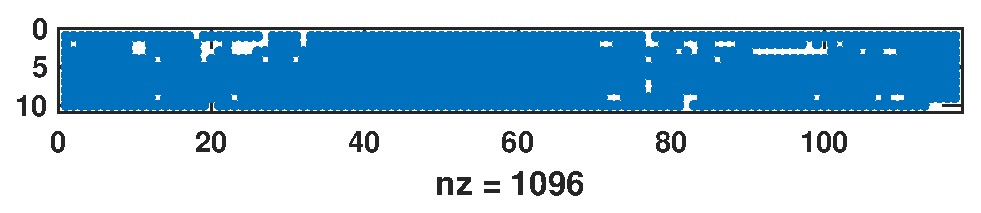
\includegraphics[width=0.8\textwidth]{original_papers/icassp_2018/figs/bat_20180710_inl.eps} \\
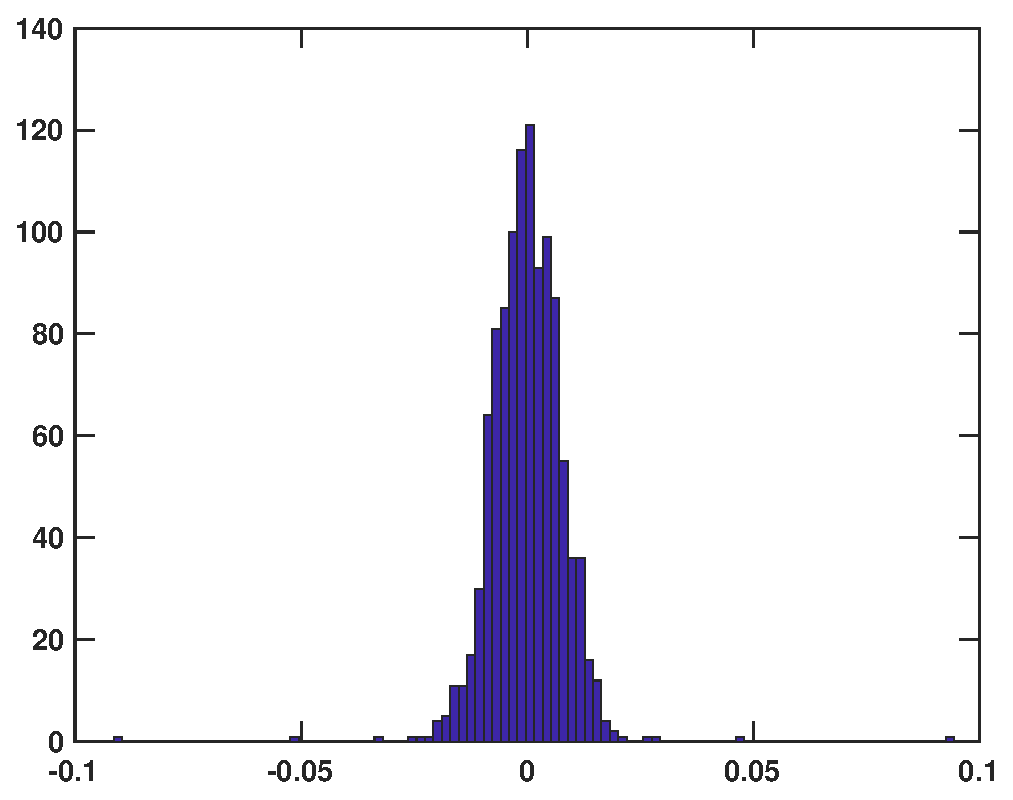
\includegraphics[width=0.4\textwidth]{original_papers/icassp_2018/figs/bat_20180710_res.eps} 
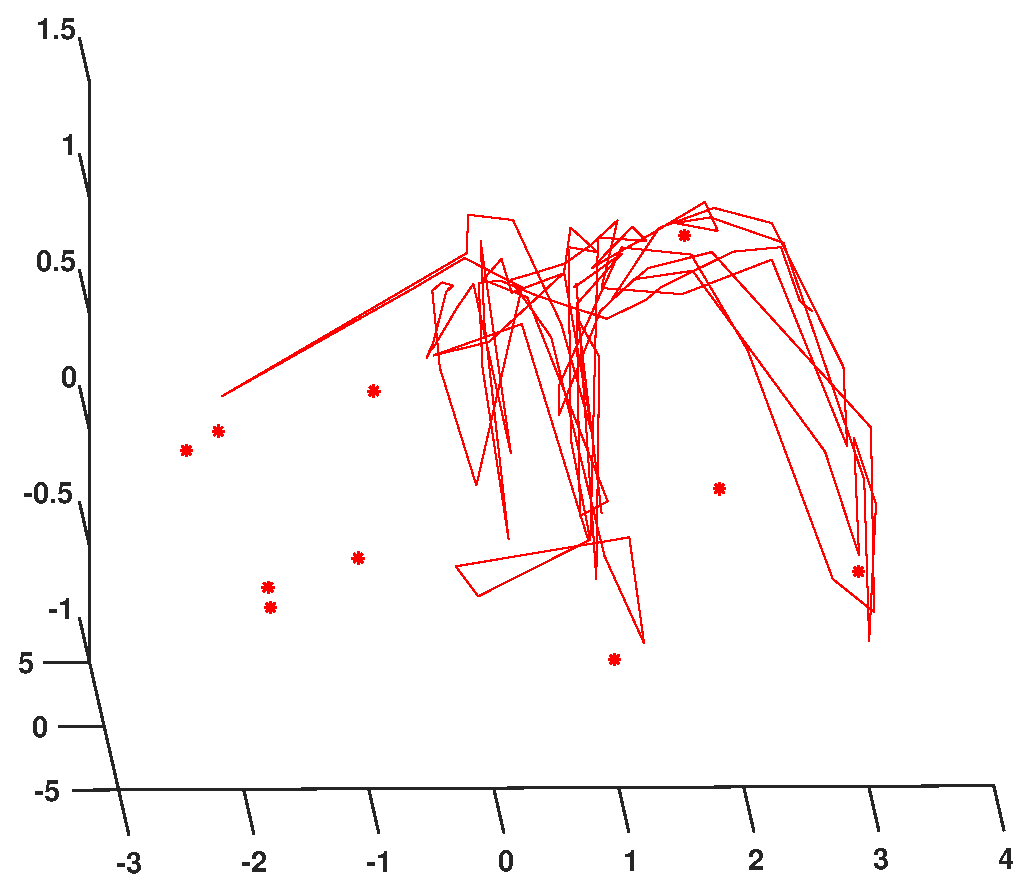
\includegraphics[width=0.4\textwidth]{original_papers/icassp_2018/figs/bat_20180710_fig.eps} \\
\end{tabular}
\caption{For the cave experiment the figure shows detected inliers $\Win$ (top), inlier residual histogram (bottom left) and  estimated microphone and sound source positions, red dots and line respectively (bottom right).}
\label{f_bat}
\end{figure}

\vspace{-5pt}
\section{Conclusions}
\label{sec:exp}
\vspace{-5pt}

In this paper, a novel method has been constructed to efficiently solve a TDOA problem with a constant offset. This has been verified using simulated data to test the solver and real experimental data to test our algorithms in realistic scenarios.

Looking at Figure \ref{fig:f_hist} and Table \ref{Tabletime}, it can be seen that the calculation of the offsets and the calculation of the relaxed form \(\theta_2\) are very fast solvers without loss in numerical accuracy. The advantage of this is that when using a RANSAC approach, the iterations are performed quickly, giving a good initial estimate in which to optimize over, which is important in highly
non-linear systems such as this.

Looking at the results from the office experiment, Figure \ref{f_454H}, we can see that the calculated microphone positions are accurate and the residuals are small, mostly in the range \(\pm 0.04~m\). Further to this our inlier set appears to be accurate. The first and last few columns (corresponding to sound emissions) are not used in our initialisation. This is correct because the recording started before the chirps were sounded and ended after, so the chirp detection algorithm falsely determined that they were also chirps but our method decided that the data in those regions do not fit the model. A comparison of the calculated microphone positions were made to a solution from a Full TDOA system, (\cite{kuang2013stratified}), which produced similar results and very similar residuals. This provided a sanity check that the chirp detection was working correctly and that from this dataset a better solution could not be found.

For the cave experiment, similar conclusions can be made, since the residuals are very low, we can conclude that we have an accurate model. This gives a real life example of how algorithms such as the one proposed can be used.

For future work, the study of the number of inliers could be of use. At the moment our algorithm may not extend to more rows and columns if the initial solution is poor, perturbing our final solution. Perhaps a method which could adapt the initial selection in order to give a required amount of inliers could be more advantageous.

\hypertarget{tacostchapter}{%
\chapter{\texorpdfstring{\texttt{tacost}: Testing and simulating the performance of acoustic tracking systems}{tacost: Testing and simulating the performance of acoustic tracking systems}}\label{tacostchapter}}

\chaptermark{Testing acoustic tracking accuracy}

This chapter was published as a preprint on \emph{biorXiv}:

\emph{Beleyur, T. (2020). \texttt{tacost}: Testing and simulating the performance of acoustic tracking systems. bioRxiv 2020.06.22.165308; doi: \url{https://doi.org/10.1101/2020.06.22.165308} }

\newpage

\hypertarget{tacostabstract}{%
\section*{Abstract}\label{tacostabstract}}
\addcontentsline{toc}{section}{Abstract}

\texttt{tacost} is a Python package to allow the testing of acoustic tracking systems. While many microphone array systems have been characterised analytically and experimentally - these are time-intensive methods. \texttt{tacost} provides a simulation based framework to rapidly assess the tracking behaviour of multiple array geometries, and the dissection of other relevant parameters. This paper explains briefly the design of the package and highlights two example use cases in which the tracking accuracy of different microphone geometries are characterised.

\newpage

\hypertarget{introduction-4}{%
\section{Introduction}\label{introduction-4}}

Acoustic tracking is a common method used to study vocalising animals such as birds, bats and cetaceans \citep{suzuki2017harkbird, aubauer1996acoustical, mohl2000sperm, Hugel2017, Holderied20032293, rhinehart2020a, blumstein2011a}.
Using acoustic tracking, biologists can detect the position of the animal and track it through space as it moves over time. The localisation accuracy of an acoustic tracking system depends on a variety of factors. There are \emph{internal} factors such as microphone array geometry, signal processing routines, and the mathematical formulations used to localise sounds (time-of-arrival, time-of-arrival-difference, angle-of-arrival, power-steering). The \emph{external} factors include aspects related to the actual signal itself, ie. signal-to-noise ratio, and spectro-temporal properties of the emitted sound (noise, linear/hyperbolic sweep) \citep{Wahlberg1999}.
While experiments and analytical modelling may be the definitive way to determine a tracking system's end accuracy, simulations allow a quick and systematic method to estimate the source of tracking errors. \texttt{tacost} provides a flexible workflow to manipulate and study the effect of both internal and external factors. \texttt{tacost} generates audio files for source positions and array geometries specified by the user. This allows the user to analyse the efficacy of their tracking system's baseline performance.

\hypertarget{statement-of-need}{%
\section{Statement of need}\label{statement-of-need}}

Generating simulated audio for a set of source sounds, positions and a given array configuration is a relatively simple task. However, to my knowledge, there are no publicly available, tested and documented packages for this task published to date. Codebases that are publicly available have the advantage of being used by a larger user-base and can thus benefit from bug discoveries much faster than in-house or individually written one-time use scripts. \texttt{tacost} provides a robust and well-documented software workflow \citep{Taschuk2016} with user and developer friendly documentation \href{https://tacost.readthedocs.io/en/latest/}{hosted online}. \texttt{tacost} contributes to the Python scientific ecosystem in the hope of promoting the growth of acoustics and bioacoustic research in open-source languages like Python. In particular, \texttt{tacost} will help researchers working in the field of acoustics and bio-acoustics \citep[eg.][]{deframond2020} plan and examine the behaviour of their acoustic tracking systems.

\hypertarget{design}{%
\section{Design}\label{design}}

The design of \texttt{tacost} focusses on a reproducible and user-friendly method \citep{Wilson2012} to generate WAV files that form the input for acoustic tracking softwares. Users may interact with \texttt{tacost} through custom-written Python scripts
by calling it as a Python package with \texttt{import\ tacost} or in the `no-coding' mode. The `no-coding' mode is especially suitable for users unfamiliar with Python. The no-coding mode is based around a parameter file that is used to specify various parts of the WAV file to be created.
Through the parameter file the user can specify the emitted sound, source positions, inter-sound-intervals, sampling rate and other relevant variables to customise the test scenario.

\hypertarget{examples}{%
\section{Examples}\label{examples}}

The localisation accuracy of a microphone array may not be uniform over 3D space \citep{aubauer1996acoustical, Wahlberg1999}. This accuracy is independent of the actual signal and recording conditions of the input data, but rather dependent on the array geometry and mathematical formulations used to record and calculate sound source position.

The accuracy of a few microphone array configurations has been characterised analytically \citep{aubauer1996acoustical} and experimentally \citep{Wahlberg1999}. While reflecting the system's capabilities, analytical
and experimental characterisations are often time-intensive. In contrast, simulation uncovers the intrinsic accuracy of an array relatively quickly through the use of audio files with simulated emission points spread across the recording volume of interest.
\texttt{tacost} can be used to characterise the maximal localisation accuracy of an acoustic tracking system with novel array geometries and recording scenarios. In Example 1, I show how \texttt{tacost} can be used to verify known trends in
localisation error with the tristar60, a commonly used array system. In Example 2, I show how \texttt{tacost} can be used to estimate the expected localisation error in a multi-microphone array with a novel and field-friendly geometry.

\hypertarget{localisation-accuracy-of-the-tristar60-system}{%
\subsection{Localisation accuracy of the tristar60 system}\label{localisation-accuracy-of-the-tristar60-system}}

The tristar60 array is a commonly used array geometry \citep{aubauer1996acoustical, Holderied20032293, Hugel2017, Lewanzik2018} with 4 microphones in a plane on an inverted T array. Three peripheral microphones are placed 120\(^{\circ}\) to each other at 60 cm radial distance from the central mic on the inverted T-array.

A series of emission points spanning the upper right quadrant of the array were simulated. The emitted sound was set to a linear sweep. The output WAV files from \texttt{tacost} were run through the TOADSuite package \citep{holger_toadsuite_manual, toadsuite_peterstilz}, a software package that localises sounds using the time-of-arrival-differences across channels. Figure \ref{tacostfig1} shows the localisation accuracy map
for the tristar60 microphone array. It can be seen (Figure \ref{tacostfig1}) that localisation error increases with increasing radial distance from the central microphone, and remains \textless7\(\%\) of the radial distance.

\begin{figure}
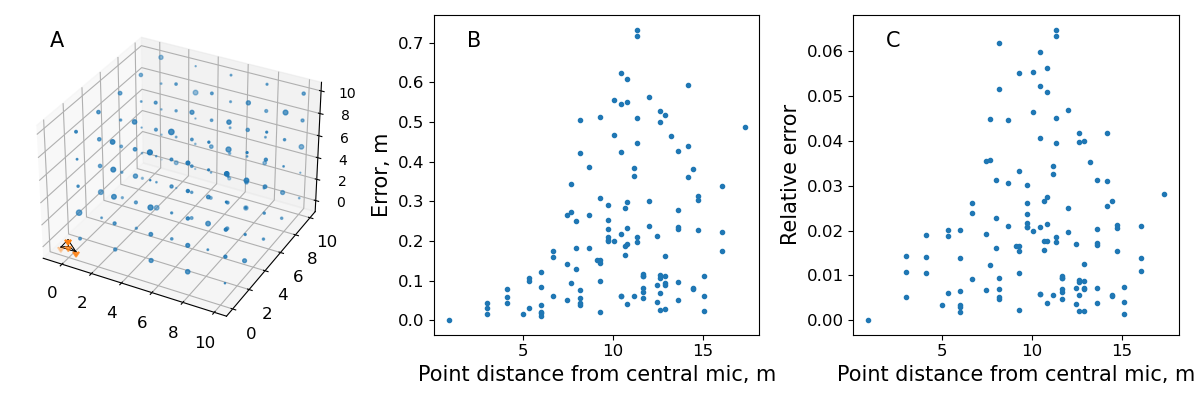
\includegraphics[width=1.0\columnwidth]{original_papers/tacost/data_for_figures/analysis/fig1_points_and_error.png}
\centering
\caption{Accuracy of a sound source localisation based on time-of-arrival-differences with a tristar60 array. A) The tristar60 microphone array is placed at the origin of the coordinate system (bottom left, orange dots connected by black lines). The blue points are the simulated source positions which form a 'calibration grid'. The size of each dot is proportional to the localisation error B) The localisation error increases with increasing radial distance of source from the central microphone. The error is the euclidean distance between the predicted and simulated source point.The errors range between 0-0.7m. C) The relative error of localisation, defined as $\frac{Localisation \:error}{Distance \:from \:central \:microphone}$. Even though absolute localisation error tends to increase with distance from array, all localisation happens with <7 $\%$ relative error.}
\label{tacostfig1}
\end{figure}

\hypertarget{localisation-accuracy-of-a-multi-microphone-array-in-the-field}{%
\subsection{Localisation accuracy of a multi-microphone array in the field}\label{localisation-accuracy-of-a-multi-microphone-array-in-the-field}}

While recording in the field, it may be difficult to use fixed arrays mounted on stands. Arrays on stands are difficult to carry and may also influence the behaviour of the animals being recorded. It is thus advantageous to use less obtrusive microphone geometries, for instance by placing microphones on pre-existing structures such as the walls of a cave or trees. These microphone geometries are field-friendly, but their localisation accuracy is hard to characterise analytically. \texttt{tacost} is an ideal tool to explore the tracking performance of such flexibly placed microphone arrays.

Figure \ref{tacostfig2}A shows the microphone array geometry and recording system described in \citep{Batstone2019}. In short, the array consisted of 11 microphones, 4 of them on a 120cm tristar, and the remaining 7 microphones attached to the walls of a cave. A series of sound emission points were created simulating points in the volume enclosed by the array. The points matched the volume echolocating bats flew within. The simulated sound was set to a linear sweep, which mimicked that of a bat call. The \texttt{tacost} output WAV files were analysed with the TOADSuite. The resulting accuracy map reveals that overall, the localisation error is between 7-30 centimetres for the given emission points. This corresponds to a maximum error of upto 30cm in tracking the position, and of upto 19\(\%\) relative error. In contrast to the previous example highlighting the increase in tracking error with increasing source sound distance, these results show a somewhat different trend. The relative error is also much higher, and it may have to do with the positioning of the sound sources in the volume with reference to the array. The relative location of the sound source affects the tracking accuracy \citep{aubauer1996acoustical}.

\begin{figure}
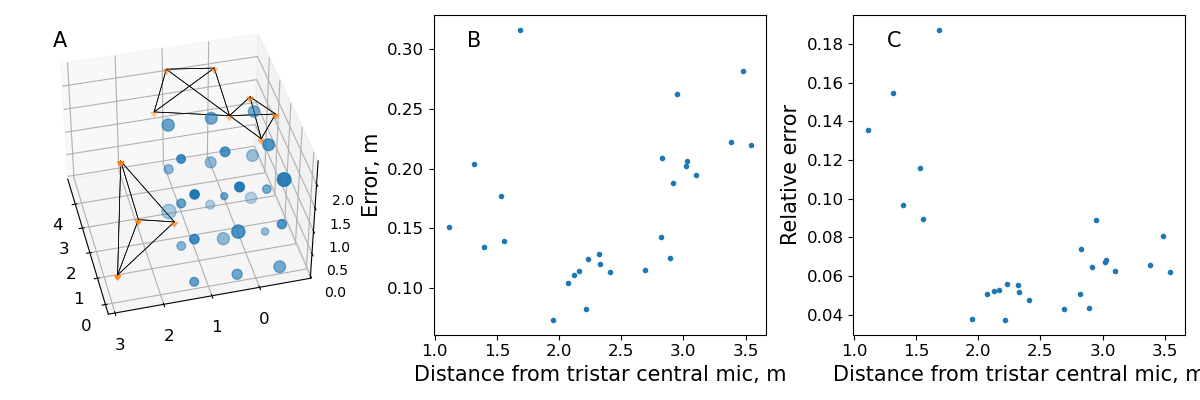
\includegraphics[width=1.0\columnwidth]{original_papers/tacost/data_for_figures/analysis/fig2_points_and_error.png}
\centering
\caption{Localisation accuracy of a multi-microphone array in the field, localised with time-of-arrival-differences. A) The line-connected points (orange) represent the microphone array consisting of 11 microphones. Four microphones are in a tristar 120 array (left, tristar array with 120cm radial distance from central mic), and 
the remaining 7 mics are placed on the walls of the cave (top right, two quadirlateral outlines joined at a common vertex represent the 7 mics on the cave walls). The free-standing points (blue) are  the simulated emission points which form a 'calibration grid'. Each simulated point is shown as a dot, and the size of the dot is proportional to the tracking error. B) The distribution of localisation error. The error is 
the euclidean distance between the predicted and simulated point. The localisation error is between 0.07-0.32 m for the given points. C) The relative localisation error with reference to the central mic of the 120 cm tristar array microphone. The 95$\%$ile bounds of tracking error lie between 3.7-16.6$\%$, with a maximum of 18.8$\%$ error. Even points that are nearby seem to be localised with a higher relative error. This higher relative error may be the result of sound source position with reference to the microphone array.}
\label{tacostfig2}
\end{figure}

\hypertarget{future-directions}{%
\section{Future directions}\label{future-directions}}

\texttt{tacost} as it stands is currently written to implement a first-order assessment of a tracking system's accuracy. The package has been primarily written keeping acoustic signals propagating through air where the velocity of sound is assumed to be constant. It may also be used to test tracking in radar or underwater sonar systems, contingent on how uniform the medium of wave propagation is over the distances being studied. As of version 0.1.0
, straight line propagation of signals are simulated, without spherical spreading or atmospheric absorption implemented. Future releases may include such propagation losses. Another important aspect affecting all tracking systems is the directionality of the sensors (microphones) and emitted signals (animal vocalisations, calibration speakers). A common problem in acoustic tracking with bats and cetaceans is not being able to track animals because their echolocation calls can be very directional \citep{Matsuta2013, Surlykke2012, Koblitz2016}. Implementing sensor and source sound directionality will help assessing how many microphones might be required to successfully track animals in their surroundings, and which array geometries are best able to do so.

\hypertarget{acknowledgements-4}{%
\section{Acknowledgements}\label{acknowledgements-4}}

This work was supported by a doctoral fellowship from the German Academic Exchange Service (DAAD) and the International Max Planck Research School for Organismal Biology.
I would like to thank Léna de Framond for generating the acoustic localisation output, Holger R Goerlitz for helpful comments on this manuscript and discussions on the topic of tracking, and the IT team at the Max-Planck Institute for Ornithology for their support.

\hypertarget{itsfmchapter}{%
\chapter{\texorpdfstring{\texttt{itsfm}, an open-source package to reliably segment and measure sounds by frequency modulation}{itsfm, an open-source package to reliably segment and measure sounds by frequency modulation}}\label{itsfmchapter}}

\chaptermark{itsfm: segmenting and measuring sounds}

This chapter was published as a preprint on \emph{biorXiv}:

\emph{Beleyur, T. (2020). \texttt{itsfm}, an open-source package to reliably segment and measure sounds by frequency modulation bioRxiv 2021.01.09.426033; doi: \url{https://doi.org/10.1101/2021.01.09.426033} }

\newpage

\hypertarget{abstractitsfm}{%
\section*{Abstract}\label{abstractitsfm}}
\addcontentsline{toc}{section}{Abstract}

Analysing animal vocalisations in detail provides insights into the biomechanics, decision making and sensory processes behind their behaviours. Echolocating bats, and in particular, the CF-FM calls of high-duty cycle bats serve as a convenient model system to illustrate this point. The CF component in the CF-FM call is used for prey detection and the FM component is used in target ranging. According to the behavioural context at hand such as flight with conspecifics or prey capture, bats choose to increase the duration, intensity or spectral range of the components differently. Studying the call component alterations requires an objective methodology that first segments the components and then allows measurements on them. Studies till now have segmented the call components manually, or automatically using what I term the `peak-frequency' method. Manual segmentation is error prone, while the `peak-frequency' method requires on-axis recordings for good results. Despite multiple papers using a peak-frequency based segmentation, there remain no publicly available software implementations. \texttt{itsfm} is an open-source package that fills this gap with two implemntations that can segment CF-FM calls, one of them being an implementation of the peak-percentage method. \texttt{itsfm} additionally introduces the `pseudo-Wigner-Ville distribution' (PWVD) method for call segmentation, thus allowing the segmentation of calls captured under a wider variety of recording conditions. I create a synthetic dataset and assess the performance of the PWVD method and the `peak-frequency' method. The PWVD performs consistently well in call component segmentation in comparison to the peak-percentage method. I also discuss the supporting methods in the \texttt{itsfm} package that can help further the automatic segmentation, measurement and analysis of sounds. Though originally developed for the segmentation and measurement of CF-FM bat calls, the methods in \texttt{itsfm} are species-agnostic, and may be used for vocalisations of any type.

\newpage

\hypertarget{introduction-5}{%
\section{Introduction}\label{introduction-5}}

Vocalisations are a window into the sensory, behavioural and biomechanical states of an animal \citep{green1979analysis, metzner2016ultrasound}. Echolocating bats present a unique model system where vocalisations play a fundamental role in the animal's sensorimotor decisions. Echolocating bats emit loud calls and listen for returning echoes to detect objects around them \citep{griffin1958listening}. Bats are known to flexibly alter various aspects of their calls to optimise echo detection, and thus their own sensory input. For instance, bats flying in the open emit long calls with a narrow bandwidth, and switch to short high-bandwidth sweeps as they are about to attack an insect prey \citep{fenton2013questions}.

Among echolocating bats, the so-called CF-FM bats are a particularly interesting model system to study sensorimotor decisions. CF-FM calls (Figure \ref{fig:cffmseg}) consist of a constant-frequency (CF) component and upto two frequency-modulated (FM) components. The CF component is used in the detection of prey wing-flutter \citep{schnitzler2011auditory} while the FM component is used in target ranging \citep{tian1997echolocation}. Bats are known to independently alter the CF and FM components depending on the presence of echolocating conspecifics \citep{fawcett2015echolocation}, artificial playbacks \citep{lu2020echolocating, hage2013ambient, hage2014ambient} or during flight manuevers \citep{tian1997echolocation, schoeppler2018precise}. Studying how CF-FM bats alter their call components requires an objective method that can reliably segment the components, and thus facilitate accurate acoustic parameter measurement.

\hypertarget{state-of-the-art-cf-fm-call-segmentation}{%
\subsection{State of the art: CF-FM call segmentation}\label{state-of-the-art-cf-fm-call-segmentation}}

Manual segmentation of calls into CF and FM is the most intuitive and direct approach one used in publications to date \citep{vater2003development, fawcett2015echolocation, gessinger2019unusual}. Manual segmentation however doesn't scale with sample size, are not very reproducible and can be biased \citep{brumm2017measurement}. \citet{tian1997echolocation} is to my knowledge, the first publication to attempt a semi-manual segmentation of the CF and FM call components, and their method has formed the founding basis for for further work. I hereby refer to methods based on their approach as the `peak percentage' approach. The `peak percentage' method relies on the fact that the CF component is at the highest frequency and forms a large part of the call. By filtering below and above a threshold frequency close to the CF frequency, the FM and CF components can be separated. In \emph{Rhinolophus ferrumequinum}, \citet{tian1997echolocation} define the threshold frequency at 0.8kHz below the 2nd harmonic of `CF component'. 0.8 kHz corresponds to around 1\% of the CF peak frequency (\textasciitilde80 kHz), and is also equivalent to filtering at 99 \% of the CF peak frequency. In their semi-manual method \citet{tian1997echolocation} measured the CF peak frequency using an FFT frequency analyser to separate FM and CF components. \citet{schoeppler2018precise} further automate the method of \citet{tian1997echolocation} by using 99\% of the CF frequency to define FM components in a spectrogram based method run on a computer. \citet{lu2020echolocating} follow on the methodology of \citet{schoeppler2018precise} and \citet{tian1997echolocation}, and set the FM to begin at 97\% of the CF peak frequency. Peak-percentage type approaches allow a straightforward segmentation and measurement, however the method was developed keeping on-axis, high signal-to-noise ratio recordings in mind, such as those that are obtained in flight room experiments. For instance, a pre-requisite for the peak-percentage method to work is a spectrally dominant CF component, in the absence of which the threshold frequency is not identified correctly, leading to poor segmentation. The peak-percentage method also requires setting a reasonable peak-percentage to define the threshold frequency that determines where the CF ends and FM begins. Previous studies have used percentages between 97-99\% of the CF peak frequency, and the exact percentage is likely to play a big role in segmentation accuracy.

Despite the widespread use of the peak-percentage method there are no openly available code implementations that have been tested for their performance against synthetic data. While code descriptions help explaining the principles behind design, it is not sufficient to ensure uniformity or correctness in implementation. Differences in implementation may lead to differences in scientific results \citep{bakervincent2019, mcfee2018open}. Publishing code as publicly available packages allows for external code inspection and improvements. \texttt{itsfm} fills the gap by implementing the peak-percentage method and introducing an alternate segmenation method. The segmentation methods are tested against synthetic datasets, with an open-source code base written in a non-proprietary language, and supported by a detailed user-guide online.

\hypertarget{package-description}{%
\section{Package description}\label{package-description}}

\texttt{itsfm} currently provides two main approaches to segment the CF and FM components of a sound (Figure \ref{fig:cffmseg}), the `peak-percentage' and `pwvd' methods.

\begin{figure}
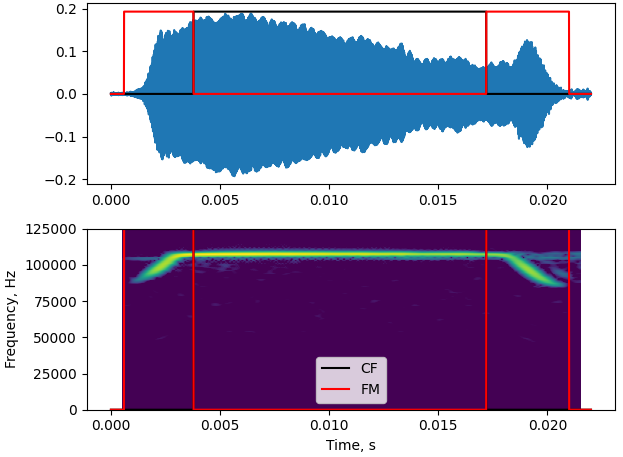
\includegraphics[width=1\linewidth]{original_papers/itsfm-paper/figures/pwvd_cffm_segmentation} \caption{Diagnostic plot showing the CF/FM segmentation output of a \textit{Rhinolophus euryale/mehelyi} call}\label{fig:cffmseg}
\end{figure}

\hypertarget{peak-percentage-segmentation}{%
\subsection{Peak-percentage segmentation}\label{peak-percentage-segmentation}}

The \texttt{peak-percentage} method is best for sounds with one or more dominant CF components of the same frequency, and FM components that are below the CF component's frequency (Figure \ref{fig:pkpctgdiags}). A typical rhinolophid/hipposiderid CF-FM call is the simplest example for which this method works. This method's implementation is inspired by previously published efforts to segment CF-FM calls into their respective components \citep{lu2020echolocating, tian1997echolocation, schoeppler2018precise}. The approach implemented here creates two versions of the raw audio that are low and high passed at a threshold frequency. The threshold frequency is calculated as a fixed percentage of the raw audio's peak frequency, eg. 99\%. The dB rms profile of the low and high passed audio are then calculated and compared by subtraction. Continuous regions where the low-passed audio is greater than the high-passed audio are considered FM regions, and CF regions where it is vice-versa (Figure \ref{fig:pkpctgdiags}).

\begin{figure}
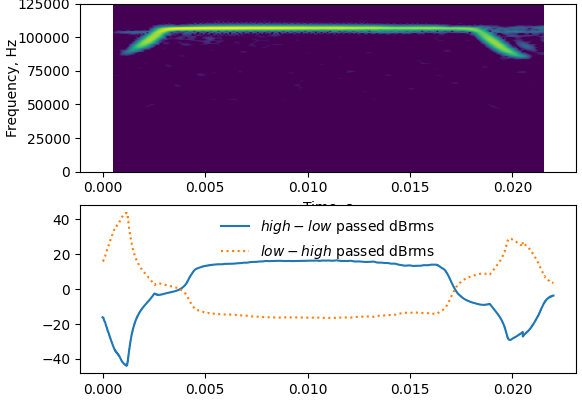
\includegraphics[width=1\linewidth]{original_papers/itsfm-paper/figures/pkpctage_profiles} \caption{Diagnostic output showing the underlying basis of the peak-percentage CF-FM segmentation method. Top: A spectrogram representation of the call shown in Figure 1, Below: the high/low-passed dB rms profiles of the call. The peak frequency of the entire call is taken and a high and low-passed version of the sound if created at 99$\%$ of the call peak frequency. The dB rms profile differences of the high and low-passed sounds are calculated and subtracted from each other. The region where the low-passed dB rms profile is higher are labelled FM and vice-versa as CF. }\label{fig:pkpctgdiags}
\end{figure}

The peak-percentage method is relatively easy to parameterise as it accepts two intuitive input parameters, the \texttt{peak\_percentage} (peak percentage value between 0-1) and \texttt{window\_size} (the number of samples for the window used to calculate the dB rms profile of the high/low passed audio). A set of additional optional parameters may also be specified. The default low/high pass filter is a second order elliptic filter with 3dB ripple (pass band) and 10dB minimum attenuation in the stop band. The user may also optionally specify their own recursive filter coefficients.

A major drawback in the peak-percentage method is its limited use-cases. Sounds must be sufficiently similar to the `ideal' spectro-temporal shape of a classic CF-FM call, or they will be mis-segmented. Not even all CF-FM calls are likely to be segmented properly, eg. CF-FM calls emitted during landing or approach with short CF segments and longer FM segments. If the CF segment of the input sound does not contribute majorly to the spectrum, then the peak-percentage method fails. Experience with field recordings having off-axis CF-FM bat calls shows that the peak-percentage method also fails here because the CF component may not be as dominant as in on-axis recordings of the same call. Aside from CF-FM echolocation calls, the peak-percentage method may also be used for certain types of bird calls with long CF and short FM calls (eg. those emitted by the \emph{Pachycephala} genus)

\hypertarget{pwvd-segmentation}{%
\subsection{PWVD segmentation}\label{pwvd-segmentation}}

The \texttt{pwvd} method (Figure \ref{fig:fmratediags}) tracks the frequency modulation over the course of the input sound. Regions with an above threshold frequency modulation are considered FM regions, and those below are considered CF regions. The frequency modulation over the course of a sound is estimated by first generating a a sample-level `frequency profile' through the use of the Pseudo Wigner-Ville Distribution (PWVD). The PWVD is a relatively underutilised method in bioacoustics \citep[but see][]{fu2018systematic, kopsinis2010time} which generates time-frequency representations with high spectro-temporal resolution \citep{boashash2015time}. The first derivative of the frequency profile is used to generate a sample-level estimate of frequency modulation and thus segment regions that are above or below the threshold.

\begin{figure}
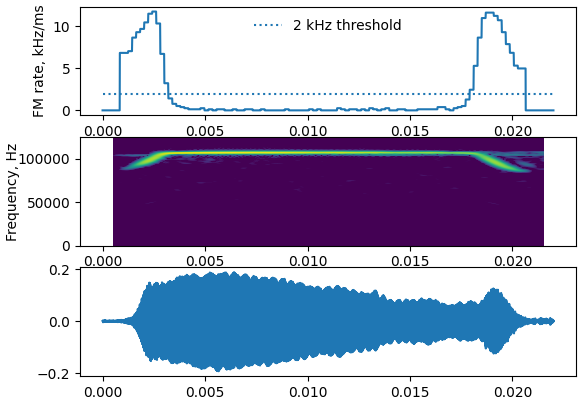
\includegraphics[width=1\linewidth]{original_papers/itsfm-paper/figures/pwvd_fmrate_diagnostic} \caption{Diagnostic plots of the pwvd method. Top: Sample-level frequency modulatation rate estimates. All regions $\geq$ the threshold FM rate (here 2kHz/ms) are considered FM regions, while all regions below this are considered CF regions. Middle-Bottom: spectrogram and waveform of the original sound for comparison.}\label{fig:fmratediags}
\end{figure}

The \texttt{pwvd} method requires somewhat more parametrisation and methodological understanding than the \texttt{peak-percentage} method. The \texttt{pwvd} method's effectiveness is dependent on the \texttt{fmrate\_threshold} (frequency modulation threshold, in kHz/ms), \texttt{pwvd\_window} size (number of samples used to form the `slices' of the time-frequency representation) and \texttt{tfr\_cliprange} (permitted dynamic range in dB, used to clip the time-frequency representation and remove noise). In addition to these primary parameters, the \texttt{pwvd} method can be further fine-tuned to improve segmentation. The frequency profile is currently generated by tracking the dominant frequency over each slice of the PWVD representation. The dominant frequency approach is susceptible to noise and changes in sound levels over time, and thus requires additional correction routines that interpolate between problematically tracked regions. The problematic regions are identified by measuring the accelaration (second derivative) of the sound's frequency profile. Regions above a user-set threshold are considered `spiky' and are interpolated or extrapolated based on neighbouring regions frequency estimates.

Even though the \texttt{pwvd} method requires some initial effort to parameterise, the flexibility it provides allows the analysis of a much wider-range of sounds than the \texttt{peak-percentage} method. The CF/FM segmentation in the \texttt{pwvd} method is independent of the actual call shape, and even complex sounds such as bat social calls and bird songs could be segmented through this method. A major drawback of the current \texttt{pwvd} implementation is its inability to reliably segment multi-harmonic sounds. Multi-harmonic sounds present a challenge for the simple frequency tracking in place currently, and alternative algorithms will be a focus of future development.

\hypertarget{supporting-itsfm-methods}{%
\subsection{\texorpdfstring{Supporting \texttt{itsfm} methods}{Supporting itsfm methods}}\label{supporting-itsfm-methods}}

Along with the primary segmentation methods, \texttt{itsfm} has a collection of supporting methods that allow quantification, visualisation and batch-processing. A series of inbuilt measurement functions allow acoustically relevant measurements such as duration, rms, peak-frequency, or terminal frequency. Custom measurements may also be specified by the user. A sound analysed with the \texttt{pwvd} method generates more than the identified CF/FM regions. Raw data on the frequency profile of the sound and the rate of frequency modulation over time are of interest to researchers studying the speed at which vocalisations can be modulated from a behavioural and biomechanical viewpoint \citep{metzner2016ultrasound, hage2013ambient}. Along with the background data used to form the segmentations, \texttt{itsfm} also provides a series of inbuilt visualisation functions to visualise the input sound itself (\texttt{visualise\_sound}) and generate diagnostic plots of the segmentation output through the \texttt{itsFMInspector} class and \texttt{visualise\_cffm\_segmentation} (Figure \ref{fig:cffmseg}).

Handling audio recordings made in the field calls for the individual handling of each recording. To aid the reproducible processing of multiple files with unique input parameters \texttt{itsfm} can also be called through a command-line interface that accepts batch files in the CSV format. To facilitate iterative parameter optimisation, the user can choose to select only a few audio recordings or the entire set of files defined in the batch file. For each processed audio file, the diagnostic plot and measurements are saved in the working directory.

The \texttt{itsfm} package also comes bundled with a series of field recordings of bat calls of various hipposiderid, rhinolophid and noctilionid species. These field recordings allow the user to test the utility of the methods in the package, and gain familiarity with setting correct parameters.

\hypertarget{methods-evaluation}{%
\section{Methods evaluation}\label{methods-evaluation}}

\hypertarget{synthetic-dataset-creation-and-segmentation}{%
\subsection{Synthetic dataset creation and segmentation}\label{synthetic-dataset-creation-and-segmentation}}

\begin{longtable}[]{@{}ll@{}}
\caption{\label{tab:synthtable} Parameter values used to generate synthetic CF-FM calls. The parameters broadly reflect the call shape of a rhinolophid/hipposiderid CF-FM bat calls. iFM and tFM regions were generated from the same FM parameter set. 9 CF x 6 iFM x 6 tFM combinations = 324 calls}\tabularnewline
\toprule
Parameter name & Values\tabularnewline
\midrule
\endfirsthead
\toprule
Parameter name & Values\tabularnewline
\midrule
\endhead
CF duration (ms) & 5, 10, 15\tabularnewline
CF peak frequency (kHz) & 40, 60, 90\tabularnewline
i/tFM duration (ms) & 1,2\tabularnewline
i/tFM bandwidth (kHz) & 5,10,20\tabularnewline
\bottomrule
\end{longtable}

To test the accuracy of the segmentation methods implemented in the \texttt{itsfm} package, I generated a set of synthetic CF-FM calls with known segment durations and spectral properties. Synthetic calls were generated based on calls broadly based on the structure of rhinolophid and hipposiderid call parameters using the package's inbuilt \texttt{make\_cffm\_call} function. A set of 324 synthetic calls were made through a combination of parameters in Table \ref{tab:synthtable}. Each synthetic call consisted of an iFM, CF and tFM component (naming as per \citep{tian1997echolocation}), and is Tukey windowed without any padded silent samples or background noise. All synthetic calls were generated at a sampling rate of 250kHz.

The synthetic calls were segmented according to method-specific parameters that were optimised based on trial-and-error on a smaller representative batch. The parameter values used for both segmentations are shown in Table \ref{tab:segparams}.

\begin{longtable}[]{@{}lllll@{}}
\caption{\label{tab:segparams} Segmentation method specific parameters used to analyse the synthetic data.}\tabularnewline
\toprule
\begin{minipage}[b]{0.16\columnwidth}\raggedright
Method\strut
\end{minipage} & \begin{minipage}[b]{0.14\columnwidth}\raggedright
Parameters\strut
\end{minipage} & \begin{minipage}[b]{0.17\columnwidth}\raggedright
\strut
\end{minipage} & \begin{minipage}[b]{0.24\columnwidth}\raggedright
\strut
\end{minipage} & \begin{minipage}[b]{0.15\columnwidth}\raggedright
\strut
\end{minipage}\tabularnewline
\midrule
\endfirsthead
\toprule
\begin{minipage}[b]{0.16\columnwidth}\raggedright
Method\strut
\end{minipage} & \begin{minipage}[b]{0.14\columnwidth}\raggedright
Parameters\strut
\end{minipage} & \begin{minipage}[b]{0.17\columnwidth}\raggedright
\strut
\end{minipage} & \begin{minipage}[b]{0.24\columnwidth}\raggedright
\strut
\end{minipage} & \begin{minipage}[b]{0.15\columnwidth}\raggedright
\strut
\end{minipage}\tabularnewline
\midrule
\endhead
\begin{minipage}[t]{0.16\columnwidth}\raggedright
pwvd\strut
\end{minipage} & \begin{minipage}[t]{0.14\columnwidth}\raggedright
Window size (samples)

\begin{verbatim}
 125
\end{verbatim}
\strut
\end{minipage} & \begin{minipage}[t]{0.17\columnwidth}\raggedright
FM rate threshold (kHz/ms)

\begin{verbatim}
   2
\end{verbatim}
\strut
\end{minipage} & \begin{minipage}[t]{0.24\columnwidth}\raggedright
Accelaration threshold (kHz/ms\(^{2}\))

10\strut
\end{minipage} & \begin{minipage}[t]{0.15\columnwidth}\raggedright
Extrapolation window(s)

75x \(10^{-6}\)\strut
\end{minipage}\tabularnewline
\begin{minipage}[t]{0.16\columnwidth}\raggedright
peak percentage\strut
\end{minipage} & \begin{minipage}[t]{0.14\columnwidth}\raggedright
Window size (samples)

\begin{verbatim}
 125
\end{verbatim}
\strut
\end{minipage} & \begin{minipage}[t]{0.17\columnwidth}\raggedright
Peak percentage

\begin{verbatim}
      0.99
\end{verbatim}
\strut
\end{minipage} & \begin{minipage}[t]{0.24\columnwidth}\raggedright
Double pass

\begin{verbatim}
   True
\end{verbatim}
\strut
\end{minipage} & \begin{minipage}[t]{0.15\columnwidth}\raggedright
\strut
\end{minipage}\tabularnewline
\bottomrule
\end{longtable}

The accuracy of segmentation was determined by comparing the duration of the obtained call components and the original values used to make the synthesied calls. The accuracy of other parameters eg. CF peak frequency, FM bandwidth was not assessed. It follows directly that if the call components have been poorly segmented, any measurements made from the underlying audio will also be unrepresentative of the actual call parameters. Some calls appeared to have more than three components due to false positive CF/FM identifications, and were not included in the accuracy calculations.

\hypertarget{results-2}{%
\subsection{Results}\label{results-2}}

The \texttt{pwvd} method correctly identified 99\% of all calls (322/324) as having only 3 components. The \texttt{peak\_percentage} method correctly identified 94\% of all calls as having 3 components (306/324). Both segmentation methods achieved a satisfactory performance. The \texttt{pwvd} method was superior in its segmentation accuracy to the \texttt{peak\_percentage} method across all the parameter combinations and call components tested (Table \ref{fig:performance}, \ref{tab:accuracypctiles}).

The relatively lower overall performance of the \texttt{peak\_percentage} method can be specifically attributed to the call properties of certain synthetic calls. A further inspection of calls with lower than 0.8 accuracy in component duration revealed that calls with a high CF frequency (60 and 90 kHz) and at least one low bandwidth FM component (5kHz) were segmented with lower accuracy. This is explained by the fact that the peak-percentage of the recursive filter is set at 0.99 of the peak frequency. A low FM bandwidth call with a high CF frequency will have its cutoff frequency much below the actual CF frequency (600 and 900 Hz below peak frequency here). The lower cutoff frequency will thus lead to a shorter duration estimate of the low-bandwidth FM component. The accuracy of component durations was above 0.8 for all calls segmented with the \texttt{pwvd} method.

One percent of all \texttt{pwvd} segmented calls and six percent of all \texttt{peak\_percentage} segmented calls had more than three detected call components. What caused the false positive call component detections in the \texttt{pwvd} and \texttt{peak\_percentage} methods? In the \texttt{peak\_percentage} method, the false component detections consisted of very short (\(\leq\) 0.1ms) falsely detected CF and FM segments located next to one another. These neighbouring CF and FM segments were caused by brief alterations in the dB rms levels of the high and low-passed audio. The brief alterations in the dB rms levels are likely due to the combination of windowing function applied on the synthetic calls and edge effects during high/low pass filtering. Such edge effects may not necessarily occur during the processing of experimentally recorded calls, which may have smoother roll-offs in call level. The two cases where false components were detected with the \texttt{pwvd} method were borderline cases where false CF components were detected in what should have been an FM region of the call. On further inspection it was shown that the frequency tracking of these false CF components was indeed accurate, but the action of the error-correction routines caused a slight drop in the frequency modulation rate to 1.9 kHz/ms, just slightly below the threshold of 2.0 kHz/ms. The error-correction routines in \texttt{pwvd} are typically required when low signal-level at the beginning and ends of the call causes jumps in the frequency tracking.

\begin{figure}
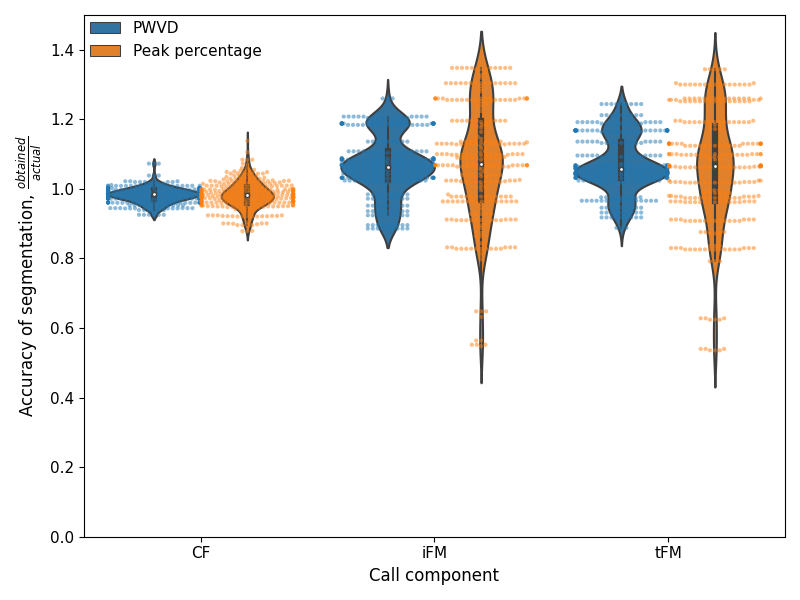
\includegraphics[width=1\linewidth]{original_papers/itsfm-paper/figures/pwvd-pkpct-comparison} \caption{\label{fig:performance} Accuracy of call component segmentation of the synthetic test data set shown with raw data overlaid on violinplots. The accuracy is calculated as the measured call component duration by the original duration. Blue violinplots: accuracy of the pwvd method, orange violinplots: accuracy of the peak-percentage method. The pwvd method is superior to the peak-percentage method in its segmentation performance across call components.}\label{fig:performance}
\end{figure}

\begin{longtable}[]{@{}lll@{}}
\caption{\label{tab:accuracypctiles} Summary statistics describing the performance of the two segmentation methods on the synthetised test data set. The pwvd method performs better than the peak-percentage method over the tested parameter space and for all call components (iFM,tFM and CF). The relative segmentation accuracy is defined as \(\frac{measured \:duration}{original \:duration}\)}\tabularnewline
\toprule
Call component & Segmentation method & Segmentation accuracy (95\(\%\)ile range)\tabularnewline
\midrule
\endfirsthead
\toprule
Call component & Segmentation method & Segmentation accuracy (95\(\%\)ile range)\tabularnewline
\midrule
\endhead
CF & peak percentage & 0.9-1.06\tabularnewline
CF & pwvd & 0.94-1.02\tabularnewline
tFM & peak percentage & 0.65-1.35\tabularnewline
tFM & pwvd & 0.89-1.21\tabularnewline
iFM & peak percentage & 0.62-1.3\tabularnewline
iFM & pwvd & 0.92-1.24\tabularnewline
\bottomrule
\end{longtable}

\hypertarget{discussion-2}{%
\section{Discussion}\label{discussion-2}}

Software based automation in acoustic analysis is an important step in ensuring reproducible results, which in turns spurs the growth of the research field \citep{mcfee2018open, bakervincent2019}. The \texttt{itsfm} package written in the Python \citep{van1995python} language is an open-sourced method which may be used in the analysis of animal vocalisations such as CF-FM bat calls, and other vocalisations. The \texttt{itsfm} package has already been successfully used to segment and measure call parameters in an upcoming publication on group echolocation in CF-FM bats \citep{hbcpaper}. The package introduces a new method the `pwvd' method to segment CF and FM components based directly on the rate of frequency modulation. The `pwvd' method also performs consistently better than the `peak-percentage' method, and is thus the recommended segmentation method to use, at least for sounds that resemble CF-FM calls.

The use of \texttt{itsfm} in the analysis of other types of vocalisations still needs further exploration. For instance, bird calls have been analysed (See \href{https://itsfm.readthedocs.io/en/latest/gallery_dir/z_bird_eg.html\#sphx-glr-gallery-dir-z-bird-eg-py}{online user-guide}). The current `pwvd' frequency tracking implementation only tracks a single frequency per point of time, and thus is not able to handle multi-harmonic sounds with equal harmonic emphasis very well. Future implementations of frequency tracking need to apply more sophisticated problem-region detection and also frequency tracking (eg. Viterbi path).

\hypertarget{open-source-software-and-packages-used}{%
\section{Open-source software and packages used}\label{open-source-software-and-packages-used}}

\texttt{itsfm} is written in the Python language \citep{van1995python}, and relies on the numpy, scipy, pandas, matplotlib and tftb \citep{numpy, 2020SciPy, matplotlib, pandas, tftb}. The Jupyter Notebook and Rmarkdown projects \citep{jupyter, rmarkdown} were used in the analysis of data and writing of this paper.

\hypertarget{supporting-information}{%
\section{Supporting information}\label{supporting-information}}

The \texttt{itsfm} package can be installed from the Python package index (PyPi) with the command \texttt{pip\ install\ itsfm}. The latest versions of the package and drafts of this paper are accessible at \url{https://github.com/thejasvibr/itsfm}. Online documentation with detailed examples and troubleshooting guides can be accessed at \url{https://itsfm.readthedocs.io}

\hypertarget{acknowledgements-5}{%
\section{Acknowledgements}\label{acknowledgements-5}}

I would like to thank Diana Schoeppler for sharing know-how on analysing CF-FM calls and Neetash Mysuru for helpful discussions. This work was funded by the DAAD and the IMPRS for Organismal Biology. I'd like to thank the following people for contributing to the call recording library Aditya Krishna, Aiqing Lin, Gloria Gessinger, Klaus-Gerhard Heller, Laura Stidsholt and Neetash Mysuru.

\hypertarget{general-discussion}{%
\chapter{General Discussion}\label{general-discussion}}

We have so far delved into detailed reports echolocation in groups, and various methodological contributions to the field. In this section I will summarise some broad points of interest, and end with my vision for future directions of study.

\hypertarget{the-cocktail-party-nightmare-a-hyperbolic-term}{%
\section{The `cocktail party nightmare': a hyperbolic term?}\label{the-cocktail-party-nightmare-a-hyperbolic-term}}

In their influential review over a decade ago \citet{ulanovsky2008a} coined the term `cocktail party nightmare' to describe the sensory challenge echolocating bats face in groups. How do individual bats manage to detect their own echoes over the deafening calls of neighbours. How to recognise one's own echoes from the constant stream of others' echoes and calls? Unable to detect echoes, a bat is devoid of sensory input and may crash into other conspecifics or obstructions. In contrast to the cocktail party problems that humans (and other animals) face, the sound levels and stakes of not detecting an echo seemed very high. The escalation from \emph{problem} to \emph{nightmare} aptly describes the perceived seriousness of group echolocation. Studies since then revealed a variety of responses that echolocators show in their call behaviour. Bats were well studied as `emitters' of signals, but understudied as `receivers'.

To understand bats as receivers in group echolocation, one must the quantify the extent to which echo detection suffers. I quantified the `cocktail party nightmare' in great detail for FM bats in Chapter \ref{cpnchapter}. The results of the model show that when in small groups echo detection is unaffected. With increasing group sizes \(\geq\) 30 however, masking plays a progressively stronger role. At group sizes of a 100 bats, a focal bat in the middle of the group can only detect at most one neighbour in front of it. To make it worse, this lone detected neighbour is only detected every third call emission, with no echoes detected the other two emissions.

Chapter \ref{cpnchapter} shows that active sensing individuals in groups have qualitatively and quantitatively different sensory inputs than passive-sensing animals. Despite occlusion, visually-dominant individuals can detect at least their nearest neighbours. My results showed that in large groups, echolocating bats may not even be able to detect their nearest neighbours every time they call.
If bats in large groups can only detect their nearest neighbour in front of them occasionally, how do echolocating animal groups show collective movements like milling, emergences or swarming? \citet{bode2011a} provide an answer with their `limited interactions' model. They show that collective movement emerges even when individuals asynchronously update their own positions with reference to just one neighbour. Their model closely mirrors what may be happening in bat groups. In our model, the echo-detection (and thus neighbour detection), is based on a simple auditory model - that did not include dynamic information processing (integration over multiple echoes), temporal gating or attentional processes. The results from the model are thus lower bound estimates of the sensory challenge a real echolocator may experiencem, and thus questions the severity of the problem real bats in groups face. In the light of results from my model, I now wonder if bats in groups perceive the cocktail party as more of a `challenge' than a nightmare?

\hypertarget{group-echolocation-need-not-always-be-taxing}{%
\section{Group echolocation need not always be taxing}\label{group-echolocation-need-not-always-be-taxing}}

The experimental study of group echolocation is centred around the echolocation responses individuals show to groups or experimental playbacks. In Chapter \ref@(hbcchapter) I investigated how CF-FM bats alter their echolocation when alone or in groups. The CF-FM bats in our study did not show major changes in their echolocation across group size. One call parameter, the dominant frequency range, even matched values from simulations recreating echolocation in groups of independent, non-responsive bats.

In contrast to many other studies, including one related species, why did our bats show no response? The `absence' of a response informs us about our expectations. Much like how I questioned the severity of FM bat group echolocation in Chapter \ref{cpnchapter}, the results in Chapter \ref{hbcchapter} also question the severity of call-echo overlaps in CF-FM bats. Call-echo overlaps are more problematic in CF-FM groups due to the long CF component. The CF component however is involved in insect wing flutter detection, and plays a role in prey capture. When performing orientation behaviour, it is highly unlikely that CF-FM bats will listen to echoes from their long CF component. Individual bats will be processing the echo's tFM component, which provides distance information. The tFM components are short (few milliseconds) and occupy a different spectral range from the CF component. Even in groups, when echoes are masked by the CF component of other bats calls, it is unlikely to prevent detection of the shorter tFM component. The multi CF-FM bat (1-4 bats) flights in our data is thus equivalent to a group of upto four FM bats echolocating together. The results of Chapter \ref{cpnchapter} tell us clearly that echo-detection is not affected at group sizes below 10 bats. Another very important reason bats may have shown no response is the high directionality of call emission in CF-FM bats, which are much more directional than FM bat calls. Intuitively, it would seem that a group of highly directional echolocators may fare better than a group of wide-beam echolocators - though this remains to be verified by modelling.

Ultimately though, it is important to stress that we studied resident bats that were likely very familiar with the cave's structure. Bats begin to rely on their spatial memory in flightrooms and as a result reduce their call rate as they spend more time flying in the room \citep{chen2015variation, yamada2020modulation, barchi2013spatial}. Bats integrate echo information from multiple calls, and have spatial memory - the combination of which may make them robust to an occasional failur in echo detection.

Field studies provide a good setting to quantify the full plethora of behaviours that animals show in `real-life' conditions. Our negative result highlights the importance of studying group echolocation in a natural setting, and adds `no response' to the variety of responses shown by bats in groups.

\hypertarget{ushichka-and-the-onward-march-of-group-echolocation-research}{%
\section{\texorpdfstring{\emph{Ushichka} and the onward march of group echolocation research}{Ushichka and the onward march of group echolocation research}}\label{ushichka-and-the-onward-march-of-group-echolocation-research}}

In Chapter \ref{ushichkachapter} I report my contribution to pushing the frontiers in the experimental study of group echolocation. Group echolocation in the field has been studied either in small groups (2-3 bats), or solely with audio or video. Animals in groups interact with each other, while also equally responding to their surroundings - like the trees, rocks or walls of a cave. Studies to date have ignored the physical environment, and only been centred on the bats themselves. Data on the simultaneous echolocation and flight behaviours of bats placed in their natural context is lacking. Having such multi-modal data provides exciting insights into the sensory inputs individuals receive, and the motor outputs they perform as a result. The trajectory and call data from \emph{Ushichka} will allow us to recreate the dynamic sensory inputs of each individual in a group. The position and call timings of individuals can be used in simulations of sound propagation to reconstruct the calls and echos originating from from neighbouring bats, and cave surfaces. While Chapter \ref{cpnchapter} recreated the sensory inputs of a bat in a group \emph{in silico}, \emph{Ushichka} provides us access to the sensory inputs of bats in a group \emph{in caverna}!

Having reconstructed the sensory inputs of bats in a group, we can then understand the sensorimotor heuristics that govern their collective motion. The collective motion and echolocation of bat groups has only been quantified in the impressive million-bat strong emergence behaviours of \emph{T. brasiliensis} to date. The \emph{T.brasiliensis} studies provide a series of findings that remain unreconciled. The bats emit extremely long calls (\(\geq\) 6 ms) in these dense emergences \citep{gillam2010a}, despite flying somewhat close to their neighbours (\textasciitilde0.5m inter-neighbour distance) \citep{theriault2010a}. This close-distance flight with long duration calls means their own emitted calls will mask returning echoes. \emph{T. brasiliensis} emergences occur around sunset like in many other species, and vision is another potential sensory modality in use. Given the call-echo masking and potential use of vision, to what extent is echolocation really being used by animals in these groups? \emph{Ushichka} provides a somewhat `cleaner' dataset into how echolocation is used in bat groups flying under pitch-black conditions of a cave system.

The bright vs dark conditions of sunset emergences and in-cave flights also brings up the question of whether different behavioural heuristics are being used. Emerging bat can potentially use both vision and echolocation, while bats in cave can only use echolocation. Can emerging bats fly at much higher densities because they can also rely on vision, or are they in fact flying at higher densities because it improves neighbour detection for echolocation (as shown in Chapter \ref{cpnchapter}), and perhaps vision as well? Better characterisation of in-cave and emergence behaviours are in need. To explain the role of different sensory modalities in collective behaviour, computational modelling of the sensory inputs available from both vision and echolocation \citep{bar2015sensory} is another promising line of investigation.

\emph{T. brasiliensis} emergences are indeed a wonder of nature, though I think we are still technologically limited in our ability to analyse the high call densities and call overlap in the audio. I believe the call densities in \emph{Ushichka} on the other hand lie in the `Goldilocks zone' of today's technology. We are neither too far from its capabilities, while the data is too easily handled by regular routines. The `middle-ness' of \emph{Ushichka} means new techniques that can handle even more complex input data can be developed. I look forward to \emph{Ushichka} becoming a centre of active inter-disciplinary collaboration, and a reference dataset for many new methodological innovations in image and signal processing, acoustic tracking, and echolocation.

\hypertarget{lowering-the-logistical-and-technical-barriers-to-group-echolocation}{%
\section{Lowering the logistical and technical barriers to (group) echolocation}\label{lowering-the-logistical-and-technical-barriers-to-group-echolocation}}

In Chapters \ref{sfscotdoa}-\ref{itsfmchapter} I presented a series of methods that promote the accuracy, automation, and ease with which echolocation in general can be studied. The \texttt{itsfm} package (Chapter \ref{itsfmchapter}) adds the `pwvd' method, a new method to segment CF-FM bat calls accurately and contributes a reference implementation for a previously described method. \texttt{tacost} (Chapter \ref{tacostchapter}) allows bioacousticians to assess the performance of their acoustic tracking system after data collection, or optimise it in the planning phase. Both packages are released under an open-source license and with detailed online documentation. The two packages are but a beginning to what I hope will be a wave of open-source bioacoustics and specifically, echolocation related packages. There still seems to be an inertia in the echolocation community when it comes to releasing code. Acoustic tracking is a central method in bat echolocation, however to my knowledge there remain no published codebases and sparse details on the software implementations. The software behind the acoustic tracking is often either closed-source licensed, or a collection of inhouse scripts with limited documentation. Both closed-source code and inhouse scripts are not welcoming of newcomers in the research community, who may not have access to the working groups concerned. It is my hope that by contributing area-specific software tools for echolocation researchers, the echolocation community may grow to realise the utility and value of openly-available packages.

In Chapter @ref(\citet{sfscotdoa}), I present the results of a collaboration towards a frame-less, measurement-free approach to acoustic tracking. In the `Structure-from-Sound' framework used in Chapter \ref{sfscotdoa}, a series of common sounds are first recorded by all microphones. The time-difference-of-arrivals across channels are then used to infer microphone positions. In many ways, this new method is the first such application to the field of echolocation. It promises a great reduction in the time spent setting up an array, and the weight of equipment to be carried into the field. I discuss more on the potential of this method in Section \ref{threepronged}.

\hypertarget{the-future-of-group-active-sensing-research}{%
\section{The future of group active sensing research}\label{the-future-of-group-active-sensing-research}}

\hypertarget{parametrising}{%
\subsection{Active sensing in other animal groups}\label{parametrising}}

The entirety of this thesis has been dedicated to the study of laryngeal-echolocating bats that emit calls between 1-100 ms long. These calls typically have a discernible spectro-temporal structure with FM or CF type components. What about other types of echolocators?
Oilbirds, swiftlets, certain fruit bats and other odontocete echolocators come to mind. Odontocetes and two species of fruit bats (\emph{Rousettus aegyptiacus} and \emph{R. leschenaulti}) emit very short `clicks' about tens to hundreds of microseconds long \citep{Fenton2014}. The probability of call-echo overlap is proportional to the duration of the calls being emitted in a group \citep{beleyur2019modeling}, and in this sense, click-based echolocators are unlikely to suffer problems detecting echoes because of call-echo (or click-echo) overlaps \citep{nelson2006a}. Oilbirds and swiflets also emit clicks, but these clicks are much closer in duration to bat echolocation calls, ranging from one to tens of milliseconds \citep{brinklov2013echolocation} - making them much more likely to suffer call-echo overlaps like bats in groups.

How click based echolocators manage to recognise their own echoes from the echoes of others is an interesting question that I think is particularly worth pursuing in the future. One strategy echolocating bats may use to recognise their own echoes is the presence of unique vocal signatures or `voices' in terms of the spectro-temporal properties or spectral emphasis in calls \citep{yovel2009voice, masters1995sonar}. Clicks however, are defined by the apparent absence of spectro-temporal structure \citep{pye1980echolocation} and their impulse-like nature (much like the clapping of the hand, or a hammer hitting a surface). Given their generally short durations I wonder if clicks carry individual-specific signatures. Of course, the absence of a `voice' in click-based echolocation doesn't preclude the use the other mechanisms that all echolocators use, such as temporal gating (using echoes that arrive within an expected time window) or using directional cues to filter out off-target echoes arriving from behind or the sides.

As receivers, all active sensing echolocators (birds and mammals) are likely to face the common problem of masking. Evidence for the occurence of masking is not new, but systematic tests in the context of echolocation have only been done in laryngeal-echolocating bats and odontocetes \citep{Nachtigall2014}. Most discussions of masking in echolocation have typically been centred around one type of masking, \emph{energetic} masking. Energetic masking, broadly defined, is when signal and masker overlap in time and frequency \citep{yost2007a, Culling2017}. Another, less discussed, type of masking is \emph{informational} masking. Informational masking occurs when signal detection is affected, despite the absence of energetic masking (no temporal or spectral overlap) \citep{Culling2017}. For instance, humans experience difficulty detecting target words in the midst of audio with two interleaved sentences. Another example is the difficulty of detecting slightly altered target tones in a background of other similar tones \citep{Kidd2017}. To my knowledge, there remain no studies of informational masking in echolocating animals - and this presents yet another unexplored facet in the study of individual and group echolocation. Here, I see the scope for the next wave of multi-species phantom echo studies \citep[eg.][]{m1989a, surlykke1992target, surlykke1996integration, siewert2004a} whose results can be directly used to construct `masking functions' (sensu \citet{beleyur2019modeling}). In general, as has been done with other animals such as birds and frogs \citep{bee2008a}, there is much potential in verifying if echolocators managing energetic and informational masking use the known strategies from human studies use such as better-ear listening and stream-segregation \citep{Culling2017}.

As emitters, active sensing animals choose how and where to focus their probe's energy \citep{Fenton2014}. Bats and odontocetes narrow or widen the `beam shape' of their emissions depending on the behaviour at hand. In essence, individuals choose to `focus' or `zoom out' their perceptual field. All studies I know of have quantified beam shapes and their modulation in solitary animals. A classic result is of bats emitting wide beam-shapes while searching for prey, narrowing onto the prey while approaching, and `zooming out' just before prey interception \citep{Fenton2014}. The direction and width of the emitted calls are direct pointers of where an animal is focussing its sensory sampling efforts. The spatial aspects of echolocation in groups remain an area of pure speculation. Do animals emit wide beams to maximise their sensory volume - and pay the costs of mutual interference? Or do they emit narrow beams focussing on the nearest objects around them - at the risk of sudden collision with an object just out of sensory range? Call overlaps and small microphone arrays have hindered beam-shape reconstruction in multi-animal groups. The study of beam shape modulations in click-emitting echolocators groups, where overlaps are rare, represents a fascinating and tractable model system.

\hypertarget{threepronged}{%
\subsection{The three-pronged approach to solve the inverse problem of group active sensing}\label{threepronged}}

The study of living things is full of inverse problems. We observe a range of fascinating phenomena, but often are unable to (and perhaps will never be able to!) recreate them under controlled settings. In this respect, biological, geological and cosmological phenomena must be tackled with a synergetic approach involving 1) pushing new technologies to generate improved measurements, 2) performing scaled-down experiments wherever possible, and finally 3) formulating computational/theoretical models that explain and predict details of the phenomenon.

In the case of active sensing, new technologies promise to lower the barrier for entry into acoustic tracking. In this thesis itself {[}Chapter \ref{sfscotdoa}{]}, we see the larval form of a field-friendly workflow for microphone position self-calibration. In its more developed form, this workflow will closely mirror current camera array calibration workflows (eg. \citet{Theriault2014}). The bioacoustician only needs to arrive at the field site and setup the microphones unobtrusively in the recording volume. To later infer the microphone positions, playbacks with a small speaker may be necessary (the animal vocalisations could themselves be used instead!). The ease and anticipatory joy of such an effortless acoustic tracking workflow can only be described by the words of a senior colleague\footnote{here's to the encouragement of Lasse Jakobsen} who said knowing there were such methods in development was the year's `Christmas gift'.

Multi-channel microphone arrays are of course typically associated with bundles of cables from the soundcard to the microphones. Cables need constant maintenance, and can in my experience, form a considerable part of equipment weight during field work. In the future, I see the scope for either wireless multi-channel recording systems, or more strategically, the potential for acoustic tracking with many independently recording devices. Acoustic tracking needs accurate time-difference of arrivals, and this has always been done so far using multi-channel soundcards that digitise data synchronously for all channels. In principle however, time-difference-of-arrivals may also be measured across two unsynchronised channels as long as the temporal offset between them is known. Similar to microphone position self-calibration, recent methods to estimate offset between asynchronous channels post-hoc \citep{burgess2012node, burgess2013minimal} promise the next methodological advance to the bioacoustician in the field. Acoustic tracking may then be done with with many smaller, cheaper and more portable recording devices. A future workflow may even include recording from hundreds to thousands of hand-held recorders in a cave, and then finally performing playbacks for cross-device synchronisation and position calibration. Groups of bats necessarily mean more complexity in the analysis of the associated data. Computer vision algorithms have made great strides into animal movement tracking, and software to reliably track hundreds to thousands of individuals is in place. On the other hand, there is still much opportunity for methodological developments in the analysis of complex audio data with overlapping sounds.

I use the term `scaled-down' experiment to mean any attempt at estimating animal capabilities under relatively controlled conditions. As described in \ref{parametrising}, many aspects of the hearing capabilities of bats and other echolocators remain unknown. My own experience with parametrising the computational model in Chapter \ref{cpnchapter} has shown me the value of multi-species studies with the same protocol. The psychophysics of only a handful of species (\emph{E. fuscus},\emph{P.pipistrellus},\emph{P.discolor}, \emph{M. lyra}) have been characterised, despite the high speciosity of bats. In flightroom studies too, a uniform protocol across species will allow for direct comparisons of results. The behavioural responses observed in flightrooms may then form the focus of field observations of much larger groups. Echolocating bats roost together in a wide continuum of group sizes \citep{kunz1982a}, and this means the extent of masking they are likely to experience will also vary. Does the species-typical group-size have an effect on the actual ability of individuals to detect masked echoes? Perhaps the robustness of echolocation to noise is more strongly affected by the environmental clutter and reverberance individuals face when commuting and hunting, rather than roosting group size per se. Studying a wider variety of species will allow us to explore the ecological and evolutionary basis of masking tolerance.

With inverse problems, modelling provides us a way to explore the feasibility of proposed mechanisms behind a phenomenon, and for well-studied phenonemna, \emph{``revise our thinking about the processes occuring''} \citep{otto2011biologist}. Despite the constant focus on sensory systems in this thesis, it is important to remember that active sensing animals are not merely `sensors'. Echolocating bats are living, breathing animals that perform rapid, well co-ordinated \emph{behaviours} using the sensory inputs they receive. Bats exhibit a host of fascinating behaviours using echolocation, including catching prey, fly long distances, care for their young, among which group flight is perhaps the most tantalising to piece-together conceptually. The bystander bioacoustician watching a mating swarm of a few hundred bats flying in a cave is only occupied by the many reasons this shouldn't even be possible in the first place! How can collective behaviours like swarming or cave emergence occur, despite the limited sensory inputs individuals receive about their neighours? For that matter, given the sophistication of bat echolocation in experimental noise, does an individual bat actually even perceive a drop in sensory input rate? Models of group echolocation \citep[eg. Chapter \ref{cpnchapter},][]{mazar2020sensorimotor} rely on the experimental input data used to parametrise them, which are often scarce. Even existing models when parametrised with new data may reveal a much more nuanced picture. Modelling may reveal that echo detection in groups occurs well, but the sensory challenge is attentional \citep{lemasson2009}, ie. to choose the most relevant echo quickly to avoid collision. Even if bats are capable of tracking the positions of all their neighbours in a group, may be they only respond to the closest one - much like the collision-avoidance heuristic shown in \citet{vanderelst2015sensorimotor}.

The three-pronged approach advocated above is of course no task for a single investigator working all alone. The approach involves a dedicated back-and-forth between disciplinary ideas, methods and people. It is my hope to have provided a cursory glimpse in this thesis of the contributions it can bring. How active sensing animals manage to aggregate and show impressive group behaviours is an exciting question that has occupied and will continue to occupy many of us in the years to come.

Meanwhile, unphased by their own abilities, the bats carry on effortlessly circling around an invisible centre in pitch-black caves and emerging in smoke-like streams in the fading light of the setting sun.

\hypertarget{acknowledgements-6}{%
\chapter{Acknowledgements}\label{acknowledgements-6}}

\emph{``An alle erschienenen und unerschienenen Erscheinungen
\newline
Menschen, Tiere, Meinungen, Gefühle, Fraktale
\newline
Zikaden, Mutanten, Schamanen, Fackelträger
\newline
Geistreisende und mikroenzyklopen-jagende Weichorganismen
\newline
Es ist an der Zeit einen Kreis zu bilden''}\footnote{To all manifested and unmanifested manifestations, humans, animals, opinions, feelings, fractals, cicadas, mutants, shamans, torchbearers, astral-travellers and microencyclope-hunting molluscs, the time has come to form a circle.}
\newline
- Käptn Peng \& Die Tentakel von Delphi, Der Anfang ist nah (The beginning is nigh)

And what a journey it has been, this Phd'fying for the past five plus years. Sitting in front of the screen right now, I never really realised how much I've relied on all the amazing people and things around me to make it this far. Let's begin, starting from the office outwards in an ever growing radius from where I sit right now.

To my office-mates: Daniel who taught me the value of a nice silent office and the joy of handling bats, Theresa - your willingness to help and chat about all things science and random, (and for introducing me to Käptn Peng). Danke Danke. To all other former and current AFEG and associated members down the corridor (Aiqing, Arun,both Claires, Dylan, Erin, Eryn, Klemen, Laura, Lena, Leo, Neetash, Stefan, Toni, Verena) thank you all for forming a great and supportive and enthu environment to come to work every day. A big shout-out to Toni for the random conversation that made the whole 2018 field season possible at all! Holger, it has been awesome working with you - and I owe you a lot for teaching me the value of good presentation and rigour in science!

Haus 11, the out-house where all the cool people are, here's to all of you current and former Haus 11'ers for the random corridor conversations and barbecue evenings! Without the Narada/Hermes/Loki messenger-like figures (who roam across the three worlds and are bearers of all kinds of knowledge and bodings) Nicole Drenkard and Diana Werner, many things would not have been possible logistically and administratively - here's a big thanks to both of you. Joerg at the Pfore : quatsch'ing with you has always been a joy every time I came to pick up chocolate or a parcel. The Max-Planck Institute for Ornithology, my place of work, I thank for having the best work-place conditions (and location) and support systems I have ever experienced. I always looked forward to arriving at work. From the people around the instit now to all things and beings around: the peaceful snow outside my window, the lake, the beautiful cycle-path to the institute, and the occasional deer eating away peacefully - I am in some way thankful to these experiences and many more that have directly or indirectly come to this point in time and space.

To my more distantly located colleagues in my graduate school, the IMPRS for Organismal Biology and all of you at the Ghetto - I thank you all for forming a supportive net to share the joy and vent the frustrations of a life in science. Special thanks to the grad school coordinators Maeggi Hieber-Ruiz, Fransisca Rosa Mende and Corinna Loes for readily providing support whenever asked for. Reni, for providing an oasis to retreat from work while Qwirkl-ing away, and Dieter for being the amazing conversationalist and story-teller he is.

My extended family in Germany: Apurva-Sindhu, Deepu-Ravi. My gratitude to you for creating a home away from home and a second base-camp over the past many years with their hospitality, food and love! Parts of this thesis literally wouldn't be written without all encouragement that came from giving me the space and time to write away in your homes along with all spiritual nourishment from the hot cups of chai and bonda-bajji's that came with it.

Neetash, for simultaneously playing the multiple roles of colleague, friend and wife over the past few years - I can not say enough, and perhaps words will not do justice! I can only be thankful that you have been by my side through the ups and downs as I tried to phd my way through to this point. Amma-Appa, for constantly supporting all my weird ideas of becoming, at various points, a vet and/or a `zoologist' (even before I actually knew what the word meant), etc! Praj - for being my go-to person in times of joy and confusion for work and life related matters. I am here only because of the unquestioning `I-have-your-back' attitude you all have shown at each point of confusion, frustration and joy in this journey till now.

And finally, I would not be here without all the bats flying through the night in lakes around and in the caves far far away in Bulgaria. All the bats that hung around as I fumbled with cables with numb hands on cold autumn nights, as I learnt to patiently deal with (hundreds of?) metres of tangled cables every night, and set up equipment hoping they'd land up. When they did it was always a pleasure to watch and hear them. So here's to all you hovercraft Daubis, hyper pipistrelles and gliding Mouse-eared bats, none of this would have been possible without all of you - and this is looking to spend more years to come understanding you weird creatures!

To everyone and everything mentioned above, and especially to all those who I have not specifically mentioned, including you my reader - I convey my gratitude: thank you, Danke,

\hypertarget{author-contributions-2}{%
\chapter{Author contributions}\label{author-contributions-2}}

Summary, General introduction and Discussion : written by Thejasvi Beleyur (TB).
Zusammenfassung translated to German by Theresa Hügel.

Chapter 2: TB and Holger R Goerlitz (HRG) conceived the study. TB formulated the computational model, wrote the code, analysed data and presented the results. TB wrote the first draft, and HRG provided input for later drafts.

Chapter 3: TB and Neetash Mysuru Rajagoplachari (NMR) conceived the study and carried out field data collection. NMR and Aditya Krishna formulated and annotated bat flights in video data. TB wrote the code to synchronise audio-video data, analysed audio, performed statistical analysis, and prepared figures. TB and NMR wrote the first draft, and HRG provided input for later drafts.

Chapter 4: TB designed and executed field data collection and wrote code to control the recording system. HRG conceived the experiment and designed the recording system. TB wrote the first draft with observations and figures, HRG provided input for later drafts.

Chapter 5: TB initiated the inter-disciplinary collaboration, carried out field data collection and wrote code to control the recording system. HRG conceived and designed the recording system. TB and HRG wrote the section describing data collection in the Orlova Chuka cave system. All other authors (Kenneth Batstone, Gabrielle Flood, Viktor Larsson, Magnus Oskarsson, Kalle Åström) were involved in the writing of other paper sections, analysis and presentation of results.

Chapter 6: TB wrote the code, analysed data, presented results and wrote the manuscript.

Chapter 7: TB wrote the code, analysed data, presented results and wrote the manuscript.

  \bibliography{beleyur-goerlitz-2020-refs.bib,tacost-references.bib,cotdoa-filtered.bib,intro-discussion-refs.bib,itsfm-references.bib,ushichka-refs.bib,hbc-references.bib}

\end{document}
